\documentclass[a4paper,adobefonts,11pt,UTF8]{book}

%type chinese characters
\usepackage{ctex}

%Bibliography
\usepackage{chapterbib}
\usepackage[sectionbib,square,super,sort&compress]{natbib}


%generate index of book
\usepackage{makeidx}

%modify the headheight at least 13.5pt
\usepackage[headheight=13.6pt]{geometry}

%
\usepackage{fontspec}

%unicode
\usepackage{xunicode}

%
\usepackage{xltxtra}

%mathematics package
\usepackage{amsmath}

%mathematics symbols
\usepackage{amssymb}

%origin print package
\usepackage{verbatim}

%draw graphics use tikz and so on.
\usepackage{graphicx}

%set graphics path which used in the book.
\graphicspath{{../img/}}

%colorful table
\usepackage{colortbl}

%set color use origin name directly.
\usepackage[svgnames,table]{xcolor}

%
\usepackage[figuresright]{rotating}

% generate longtable which could across pages.
\usepackage{longtable}

\usepackage{lscape}

%
\usepackage{multirow}

%
\usepackage{adjustbox}


%
\newcommand\mgape[1]{\gape{$\vcenter{\hbox{#1}}$}}

%
\usepackage{array}

%
\usepackage{makecell}

%
\usepackage{ulem}

%
\usepackage{color}

% draw graphics use tikz package
\usepackage{tikz}

%
\usepackage{listings}
\lstset{
  basicstyle=\ttfamily\small,
  showstringspaces=false,
  commentstyle=\color{red},
  keywordstyle=\color{blue},
  columns=flexible,
  backgroundcolor=\color{lightgray},
  extendedchars=true,
  basicstyle=\footnotesize\ttfamily,
  showstringspaces=false,
  showspaces=false,
  %numbers=left,
  %numberstyle=\footnotesize,
  %numbersep=9pt,
  tabsize=2,
  breaklines=true,
  showtabs=false,
  captionpos=b
}

%
\usepackage{bashful}

%set book information including bookmarksnumbered,pdfencoding,
%pdfauthor,pdfpagelayout,breaklinks,colorlinks,linkcolor,
%urlcolor,and so on.
\usepackage[bookmarksnumbered,pdfencoding=auto,pdfauthor={穷屌丝联盟},pdfpagelayout=TwoPageRight,breaklinks,colorlinks,linkcolor=RoyalBlue,urlcolor=blue,colorlinks=true]{hyperref}

%add more list types.
\usepackage{paralist}

%set page styles
\usepackage{fancyhdr}

\pagestyle{fancy}
\fancyhf{}
\fancyhead[LE,RO]{\thepage}
\fancyhead[RE]{\leftmark}
\fancyhead[RO]{\rightmark}
\fancypagestyle{plain}{
  \fancyhf{}
  \renewcommand{\headrulewidth}{0pt}
}


%titlepage \titleGM
\newcommand*{\plogo}{\fbox{$\mathcal{PL}$}} % Generic publisher logo
%--------------------------------------------------------------------
% TITLE PAGE
%--------------------------------------------------------------------

\newcommand*{\titleGM}{\begingroup % Create the command for including the title page in the document
\hbox{ % Horizontal box
\hspace*{0.2\textwidth} % Whitespace to the left of the title page
\rule{1pt}{\textheight} % Vertical line
\hspace*{0.05\textwidth} % Whitespace between the vertical line and title page text
\parbox[b]{0.75\textwidth}{ % Paragraph box which restricts text to less than the width of the page
{\noindent\Huge\bfseries Notes Collection of \\[0.5\baselineskip] Web Development}\\[2\baselineskip] % Title
{\large \textit{Web Development}}\\[4\baselineskip] % Tagline or further description
{\Large \textsc{theqiong.com}} % Author name

\vspace{0.5\textheight} % Whitespace between the title block and the publisher
{\noindent 穷屌丝联盟}\\[\baselineskip] % Publisher and logo
}}
\endgroup}
%


%lstlisting[language=JavsScript]
% Taken from Lena Herrmann at 
% http://lenaherrmann.net/2010/05/20/javascript-syntax-highlighting-in-the-latex-listings-package
\definecolor{lightgray}{rgb}{.99,.99,.99}
\definecolor{darkgray}{rgb}{.4,.4,.4}
\definecolor{purple}{rgb}{0.65,0.12,0.82}

%lstlisting package -----------
% JavaScript
%------------------------------
\lstdefinelanguage{JavaScript}
{
  keywords={typeof,new,ture,false,catch,function,return,null,switch,var,if,in,while,do,else,case,break},
  keywordstyle=\color{blue}\bfseries,
  ndkeywords={class,export,boolean,throw,implements,import,this},
  ndkeywordstyle=\color{darkgray}\bfseries,
  identifierstyle=\color{black},
  sensitive=false,
  comment=[l]{//},
  morecomments[s]{/*}{*/},
  commentstyle=\color{purple}\ttfamily,
  stringstyle=\color{red}\ttfamily,
  morestring=[b]',
  morestring=[b]"
}

\lstdefinelanguage{Scheme}
{morekeywords={,lambda, cond, case, display, let, import, quote, quasiquote, unquote,
define, begin, newline, if, list, apply, null?, car, cdr, or, not, and, for-each, 
make-vector, vector-length, vector-ref, vector-set!, eqv?, eq?, equal?, else, set!, 
define-record-type, fields, mutable, immutable, assert, parent, with-exception-handler, }
sensitive=false,
morecomment=[l]{;},
morecomment=[s]{/*}{*/},
morestring=[b]",
}

\lstdefinelanguage{CSS}{
  morekeywords={accelerator,azimuth,background,background-attachment,
    background-color,background-image,background-position,
    background-position-x,background-position-y,background-repeat,
    behavior,border,border-bottom,border-bottom-color,
    border-bottom-style,border-bottom-width,border-collapse,
    border-color,border-left,border-left-color,border-left-style,
    border-left-width,border-right,border-right-color,
    border-right-style,border-right-width,border-spacing,
    border-style,border-top,border-top-color,border-top-style,
    border-top-width,border-width,bottom,caption-side,clear,
    clip,color,content,counter-increment,counter-reset,cue,
    cue-after,cue-before,cursor,direction,display,elevation,
    empty-cells,filter,float,font,font-family,font-size,
    font-size-adjust,font-stretch,font-style,font-variant,
    font-weight,height,ime-mode,include-source,
    layer-background-color,layer-background-image,layout-flow,
    layout-grid,layout-grid-char,layout-grid-char-spacing,
    layout-grid-line,layout-grid-mode,layout-grid-type,left,
    letter-spacing,line-break,line-height,list-style,
    list-style-image,list-style-position,list-style-type,margin,
    margin-bottom,margin-left,margin-right,margin-top,
    marker-offset,marks,max-height,max-width,min-height,
    min-width,-moz-binding,-moz-border-radius,
    -moz-border-radius-topleft,-moz-border-radius-topright,
    -moz-border-radius-bottomright,-moz-border-radius-bottomleft,
    -moz-border-top-colors,-moz-border-right-colors,
    -moz-border-bottom-colors,-moz-border-left-colors,-moz-opacity,
    -moz-outline,-moz-outline-color,-moz-outline-style,
    -moz-outline-width,-moz-user-focus,-moz-user-input,
    -moz-user-modify,-moz-user-select,orphans,outline,
    outline-color,outline-style,outline-width,overflow,
    overflow-X,overflow-Y,padding,padding-bottom,padding-left,
    padding-right,padding-top,page,page-break-after,
    page-break-before,page-break-inside,pause,pause-after,
    pause-before,pitch,pitch-range,play-during,position,quotes,
    -replace,richness,right,ruby-align,ruby-overhang,
    ruby-position,-set-link-source,size,speak,speak-header,
    speak-numeral,speak-punctuation,speech-rate,stress,
    scrollbar-arrow-color,scrollbar-base-color,
    scrollbar-dark-shadow-color,scrollbar-face-color,
    scrollbar-highlight-color,scrollbar-shadow-color,
    scrollbar-3d-light-color,scrollbar-track-color,table-layout,
    text-align,text-align-last,text-decoration,text-indent,
    text-justify,text-overflow,text-shadow,text-transform,
    text-autospace,text-kashida-space,text-underline-position,top,
    unicode-bidi,-use-link-source,vertical-align,visibility,
    voice-family,volume,white-space,widows,width,word-break,
    word-spacing,word-wrap,writing-mode,z-index,zoom},
  morestring=[s]{:}{;},
  sensitive,
  morecomment=[s]{/*}{*/}
}








\setmainfont[Mapping=tex-text]{Minion Pro}

\makeindex\makeindex


\title{Web Development Notes}
\author{穷屌丝联盟\\ \texttt{theqiong.com}}
\date{\today}

\begin{document}

\begin{titlepage}
\addcontentsline{toc}{part}{Cover}

\pagestyle{empty} % Removes page numbers

\titleGM % This command includes the title page


\end{titlepage}

\maketitle
\tableofcontents
\listoffigures
\listoftables
\printindex


\part{Introduction}



Web development\cite{web_development} is a broad term for the work involved in developing a web site for the Internet (World Wide Web) or an intranet (a private network). Web development can range from developing the simplest static single page of plain text to the most complex web-based internet applications, electronic businesses, and social network services. A more comprehensive list of tasks to which web development commonly refers, may include web design, web content development, client liaison, client-side/server-side scripting, web server and network security configuration, and e-commerce development. Among web professionals, "web development" usually refers to the main non-design aspects of building web sites: writing markup and coding.

For larger organizations and businesses, web development teams can consist of hundreds of people (web developers). Smaller organizations may only require a single permanent or contracting webmaster, or secondary assignment to related job positions such as a graphic designer and/or information systems technician. Web development may be a collaborative effort between departments rather than the domain of a designated department..

Since the commercialization of the web, web development has been a growing industry. The growth of this industry is being pushed especially by businesses wishing to sell products and services to online customers.


For tools and platforms, the public can use many open source systems to aid in web development. A popular example, the LAMP (Linux, Apache, MySQL, PHP) stack is available for download online free of charge. This has kept the cost of learning web development to a minimum. Another contributing factor to the growth of the industry has been the rise of easy-to-use WYSIWYG web-development software, most prominently Adobe Dreamweaver, WebDev, and Microsoft Expression Studio. Using such software, virtually anyone can relatively quickly learn to develop a very basic web page. Knowledge of HyperText Markup Language (HTML) or of programming languages is still required to use such software, but the basics can be learned and implemented quickly with the help of help files, technical books, internet tutorials, or face-to-face training.

An ever growing set of tools and technologies have helped developers build more dynamic and interactive websites. Web developers now help to deliver applications as web services which were traditionally only available as applications on a desk-based computer.

Instead of running executable code on a local computer, users can interact with online applications to create new content. This has created new methods in communication[citation needed] and allowed for many opportunities to decentralize information and media distribution. Users can interact with applications from many locations, instead of being tied to a specific workstation for their application environment.

Examples of dramatic transformation in communication and commerce led by web development include e-commerce. Online auction-sites such as eBay have changed the way consumers find and purchase goods and services. Online retailers such as Amazon.com and Buy.com (among many others) have transformed the shopping and bargain-hunting experience for many consumers. Another good example of transformative communication led by web development is the blog. Web applications such as WordPress and Movable Type have created easily-implemented blog-environments for individual web sites. The popularity of open-source content management systems such as Joomla!, Drupal, XOOPS, and TYPO3 and enterprise content management systems such as Alfresco have extended web development's impact at online interaction and communication.

Web development has also impacted personal networking and marketing. Websites are no longer simply tools for work or for commerce, but serve more broadly for communication and social networking. Websites such as Facebook and Twitter provide users with a platform to communicate and organizations with a more personal and interactive way to engage the public.

Web开发是指使用网页设计程序语言设计交互式的网页,又称动态网页,动态网页是指网页的内容是否可根据某种条件的改变而自动改变,如计数器就是动态的,当有人点击我们的网页时,计数器的值会自动增加;BBS论坛也是动态的,当用户在论坛上发布信息时,网页内容会自动更新,显示出新发布的信息及相关回复;等等。需要注意的是GIF动画和Flash动画是静态的。因为,这些动画一旦制作完成后,就不会再改变了,尽管Flash动画可以响应用户的事件。


Web Development can be split into many areas and a typical and basic web development hierarchy might consist of:

\begin{compactitem}
\item Client side coding

\begin{compactitem}
\item \href{http://en.wikipedia.org/wiki/Ajax_(programming)}{Ajax}

Asynchronous JavaScript provides new methods of using JavaScript, and other languages to improve the user experience.
\item \href{http://en.wikipedia.org/wiki/Adobe_Flash}{Flash}

Adobe Flash Player is a ubiquitous browser plugin ready for RIAs. Flex 2 is also deployed to the Flash Player (version 9+).
\item \href{http://en.wikipedia.org/wiki/JavaScript}{JavaScript}

JavaScript is a ubiquitous client side platform for creating and delivering rich web applications that can also run across a wide variety of devices. It is a dialect of the scripting language ECMAScript.
\item \href{http://en.wikipedia.org/wiki/JQuery}{jQuery}

Cross-browser JavaScript library designed to simplify and speed up the client-side scripting of HTML.
\item \href{http://en.wikipedia.org/wiki/Microsoft_Silverlight}{Microsoft Silverlight}

Microsoft's browser plugin that enables animation, vector graphics and high-definition video playback, programmed using XAML and .NET programming languages.
\item \href{http://en.wikipedia.org/wiki/HTML5}{HTML5} and \href{http://en.wikipedia.org/wiki/CSS3}{CSS3}

Latest HTML proposed standard combined with the latest proposed standard for CSS natively supports much of the client-side functionality provided by other frameworks such as Flash and Silverlight
\end{compactitem}

Looking at these items from an "umbrella approach", client side coding such as XHTML is executed and stored on a local client (in a web browser) whereas server side code is not available to a client and is executed on a web server which generates the appropriate XHTML which is then sent to the client. The nature of client side coding allows you to alter the HTML on a local client and refresh the pages with updated content (locally), web designers must bear in mind the importance and relevance to security with their server side scripts. If a server side script accepts content from a locally modified client side script, the web development of that page is poorly sanitized with relation to security.

\item Server side coding

\begin{compactitem}
\item ASP (Microsoft proprietary)
\item ActiveVFP (open source)
\item CSP, Server-Side ANSI C
\item ColdFusion (Adobe proprietary, formerly Macromedia, formerly Allaire)
\item CGI
\item Erlang, with Linux, Yaws, Mnesia, Erlang (LYME) solution stack
\item Groovy, using the Grails framework
\item Java, e.g. Java EE or WebObjects
\item Lotus Domino
\item Node.js
\item Perl, e.g. Catalyst, Dancer or Mojolicious (all open source)
\item PHP (open source)
\item Python, e.g. Django (web framework) (open source)
\item Real Studio Web Edition
\item Ruby, e.g. Ruby on Rails (open source)
\item Smalltalk e.g. Seaside, AIDA/Web
\item SSJS Server-Side JavaScript, e.g. Aptana Jaxer, Mozilla Rhino
\item WebDNA (WSC proprietary)
\item Websphere (IBM proprietary)
\item .NET and .NET MVC Frameworks (Microsoft proprietary)
\end{compactitem}


\item Client side + server side

\begin{compactitem}
\item Google Web Toolkit provides tools to create and maintain complex JavaScript front-end applications in Java.
\item Dart provides tools to create and maintain complex JavaScript front-end applications as well as supporting server-side code in Dart (programming language).
\item Opa is a high-level language in which both the client and the server parts are implemented. The compiler then decides which parts run on the client (and are translated automatically to JavaScript) and which parts run on the server. The developer can tune those decisions with simple directives. (open source)
\item Pyjamas is a tool and framework for developing Ajax applications and Rich Internet Applications in python.
\item Tersus is a platform for the development of rich web applications by visually defining user interface, client side behavior and server side processing. (open source)
\end{compactitem}

However languages like Ruby and Python are often paired with database servers other than MySQL (the M in LAMP). Below are example of other databases currently in wide use on the web. For instance some developers prefer a LAPR(Linux/Apache/PostgreSQL/Ruby on Rails) setup for development.

\item Database technology

\begin{compactitem}
\item FileMaker
\item Apache Derby
\item IBM DB2
\item Firebird
\item Microsoft SQL Server
\item MySQL
\item Oracle
\item PostgreSQL
\item SQLite
\item Sybase
\item WebDNA
\item Redis
\item MongoDB
\item CouchDB
\item Mark\_Logic
\end{compactitem}


\end{compactitem}

The World Wide Web has become a major delivery platform for web development a variety of complex and sophisticated enterprise applications in several domains. In addition to their inherent multifaceted functionality, these web applications exhibit complex behavior and place some unique demands on their usability, performance, security and ability to grow and evolve. However, a vast majority of these applications continue to be developed in an ad-hoc way, contributing to problems of usability, maintainability, quality and reliability.(1)(2) While web development can benefit from established practices from other related disciplines, it has certain distinguishing characteristics that demand special considerations. In recent years of web development there have been some developments towards addressing these problems and requirements. As an emerging discipline, web engineering actively promotes systematic, disciplined and quantifiable approaches towards successful development of high-quality, ubiquitously usable web-based systems and applications.(3)(4) In particular, web engineering focuses on the methodologies, techniques and tools that are the foundation of web application development and which support their design, development, evolution, and evaluation. Web application development has certain characteristics that make it different from traditional software, information system, or computer application development.

Web engineering is multidisciplinary and encompasses contributions from diverse areas: systems analysis and design, software engineering, hypermedia/hypertext engineering, requirements engineering, human-computer interaction, user interface, information engineering, information indexing and retrieval, testing, modelling and simulation, project management, and graphic design and presentation. Web engineering is neither a clone, nor a subset of software engineering, although both involve programming and software development. While web engineering uses software engineering principles, web development encompasses new approaches, methodologies, tools, techniques, and guidelines to meet the unique requirements for web-based applications.


\chapter{Practical web development}


In practice, many web developers will have basic interdisciplinary skills / roles, including:

\begin{compactitem}
\item Graphic design / web design
\item Information architecture and copywriting/copyediting with web usability, accessibility and search engine optimization in mind
\end{compactitem}


The above list is a simple website development hierarchy and can be extended to include all client side and server side aspects. It is still important to remember that web development is generally split up into client side coding, covering aspects such as the layout and design, and server side coding, which covers the website's functionality and back-end systems.

Some more advanced web developers will also have these interdisciplinary skills / roles:

\begin{compactitem}
\item GUI (Graphic User Interface) design
\item Audio, Video and Animation processing \& encoding (for web usage)
\item Flash Capabilities (animation, audio, video, scripting)
\item Web content management system Deployment and/or Content management infrastructure design, development and integration
\item Web applications development, integration and deployment
\item Web server stress testing (how much traffic can a web server running a specific application endure before collapsing)
\item Web site security analysis \& testing
\item Web site code optimization (which is an important aspect of search engine optimization)
\item Project management, QA and other aspects common to IT development
\end{compactitem}


Netscape introduced an implementation of JavaScript for server-side scripting with Netscape Enterprise Server, first released in December, 1994 (soon after releasing JavaScript for browsers).

Server-side scripting was later used in early 1995 by Fred DuFresne while developing the first web site for Boston, MA television station WCVB. The technology is described in US patent 5835712. The patent was issued in 1998 and is now owned by Open Invention Network (OIN). In 2010 OIN named Fred DuFresne a "Distinguished Inventor" for his work on server-side scripting.


In the earlier days of the web, server-side scripting was almost exclusively performed by using a combination of C programs, Perl scripts, and shell scripts using the Common Gateway Interface (CGI). Those scripts were executed by the operating system, and the results were served back by the web server. Many modern web servers can directly execute on-line scripting languages such as ASP and PHP either by the web server itself or via extension modules (e.g. mod\_perl or mod\_php) to the web server. For example, WebDNA includes its own embedded database system. Either form of scripting (i.e., CGI or direct execution) can be used to build up complex multi-page sites, but direct execution usually results in lower overhead due to the lack of calls to external interpreters.

Dynamic websites sometimes use custom web application servers, such as the Python "Base HTTP Server" library, although some may not consider this to be server-side scripting. When designing using dynamic web-based scripting technics, like classic ASP or PHP, developers must have a keen understanding of the logical, temporal, and physical separation between the client and the server. For a user's action to trigger the execution of server-side code, for example, a developer working with classic ASP must explicitly cause the user's browser to make a request back to the web server. Creating such interactions can easily consume much development time and lead to unreadable code.



\section{Client-side scripting}


Client-side scripting\cite{client_side_scripting} generally refers to the class of computer programs on the web that are executed client-side, by the user's web browser, instead of server-side (on the web server).[1] This type of computer programming is an important part of the Dynamic HTML (DHTML) concept, enabling web pages to be scripted; that is, to have different and changing content depending on user input, environmental conditions (such as the time of day), or other variables.

Client-side scripts are often embedded within an HTML or XHTML document (hence known as an "embedded script"), but they may also be contained in a separate file, to which the document (or documents) that use it make reference (hence known as an "external script"). Upon request, the necessary files are sent to the user's computer by the web server (or servers) on which they reside. The user's web browser executes the script, then displays the document, including any visible output from the script. Client-side scripts may also contain instructions for the browser to follow in response to certain user actions, (e.g., clicking a button). Often, these instructions can be followed without further communication with the server.

By viewing the file that contains the script, users may be able to see its source code. Many web authors learn how to write client-side scripts partly by examining the source code for other authors' scripts.

In contrast, server-side scripts, written in languages such as Perl,Python,PHP, ASP.NET, Java, and server-side VBScript, are executed by the web server when the user requests a document. They produce output in a format understandable by web browsers (usually HTML), which is then sent to the user's computer. The user cannot see the script's source code (unless the author publishes the code separately), and may not even be aware that a script was executed. Documents produced by server-side scripts may, in turn, contain client-side scripts.

Server-side scripts require that their language's interpreter be installed on the server, and produce the same output regardless of the client's browser, operating system, or other system details. Client-side scripts do not require additional software on the server (making them popular with authors who lack administrative access to their servers); however, they do require that the user's web browser understands the scripting language in which they are written. It is therefore impractical for an author to write scripts in a language that is not supported by popular web browsers.

Due to security restrictions, client-side scripts may not be allowed to access the user's computer beyond the web browser application. Techniques like ActiveX controls can be used to sidestep this restriction.

Client-side scripting is not inherently unsafe. Users are encouraged to always keep their web browsers up-to-date to avoid exposing their computer and data to vulnerabilities that are discovered.

The latest group of web browsers and web pages tend to employ a heavy amount of client-side scripting, accounting for an improved user interface in which the user does not experience the unfriendly "refreshing" of the web page, but instead sees perhaps an animated GIF file indicating that the request occurred and the page will be updated shortly. Ajax is an important addition to the JavaScript language, allowing web developers to communicate with the web server in the background without requiring a completely new version of the page to be requested and rendered. This leads to a much improved user experience in general.

Unfortunately, even languages that are supported by a wide variety of browsers may not be implemented in precisely the same way across all browsers and operating systems. Authors are well-advised to review the behavior of their client-side scripts on a variety of platforms before they put them into use.


\section{Server-side scripting}

Server-side scripting\cite{sever_side_scripting} is a technique used in website design which involves embedding scripts in an HTML source code which results in a user's (client's) request to the server website being handled by a script running server-side before the server responds to the client's request. The scripts can be written in any of a number of server-side scripting languages available (see below). Server-side scripting differs from client-side scripting where embedded scripts, such as JavaScript, are run client-side in the web browser.

Server-side scripting is usually used to provide an interface and to limit client access to proprietary databases or other data sources. These scripts may assemble client characteristics for use in customizing the response based on those characteristics, the user's requirements, access rights, etc. Server-side scripting also enables the website owner to reduce user access to the source code of server-side scripts which may be proprietary and valuable in itself. The down-side to the use of server-side scripting is that the server website computer needs to provide most of the computing resources before sending a page to the client computer for display via its web browser.

When the server serves data in a commonly used manner, for example according to the HTTP or FTP protocols, users may have their choice of a number of client programs (most modern web browsers can request and receive data using both of those protocols). In the case of more specialized applications, programmers may write their own server, client, and communications protocol, that can only be used with one another.

Programs that run on a user's local computer without ever sending or receiving data over a network are not considered clients, and so the operations of such programs would not be considered client-side operations.

There are a number of server-side scripting languages available, including:

\begin{compactitem}
\item ASP (*.asp)
\item ActiveVFP (*.avfp)
\item ASP.NET (*.aspx)
\item C via CGI (*.c, *.csp)
\item ColdFusion Markup Language (*.cfm)
\item Java via JavaServer Pages (*.jsp)
\item JavaScript using Server-side JavaScript (*.ssjs, *.js) (example: Node.js)
\item Lua (*.lp *.op *.lua)
\item Perl CGI (*.cgi, *.ipl, *.pl)
\item PHP (*.php) - Open Source Scripting
\item R (*.rhtml) - via rApache
\item Python, e.g. via Django (*.py)
\item Ruby, e.g. Ruby on Rails (*.rb, *.rbw)
\item SMX (*.smx)
\item Lasso (*.lasso)
\item Tcl (*.tcl)
\item WebDNA (*.dna,*.tpl)
\item Progress WebSpeed (*.r,*.w)
\end{compactitem}



\section{Security considerations}


Web development takes into account many security considerations, such as data entry error checking through forms, filtering output, and encryption.[2] Malicious practices such as SQL injection can be executed by users with ill intent yet with only primitive knowledge of web development as a whole. Scripts can be used to exploit websites by granting unauthorized access to malicious users that try to collect information such as email addresses, passwords and protected content like credit card numbers.

Some of this is dependent on the server environment (most commonly Apache or Microsoft IIS) on which the scripting language, such as PHP, Ruby, Python, Perl or ASP is running, and therefore is not necessarily down to the web developer themselves to maintain. However, stringent testing of web applications before public release is encouraged to prevent such exploits from occurring. If some contact form is provided in a website it should include a captcha field in it which prevents computer programs from automatically filling forms and also mail spamming.

Keeping a web server safe from intrusion is often called Server Port Hardening. Many technologies come into play to keep information on the internet safe when it is transmitted from one location to another. For instance Secure Socket Layer Encryption (SSL) Certificates are issued by certificate authorities to help prevent internet fraud. Many developers often employ different forms of encryption when transmitting and storing sensitive information. A basic understanding of information technology security concerns is often part of a web developer's knowledge.

Because new security holes are found in web applications even after testing and launch, security patch updates are frequent for widely used applications. It is often the job of web developers to keep applications up to date as security patches are released and new security concerns are discovered.


\chapter{Web Document}

A web document\cite{web_document} is similar in concept to a web page, but also satisfies the following broader definition by W3C:


\fbox{
	\parbox[c][180pt][c]{350pt}{\noindent \textbf{``... Every Web document has its own URI. Note that a Web document is not the same as a file: a single Web document can be available in many different formats and languages, and a single file, for example a PHP script, may be responsible for generating a large number of Web documents with different URIs. A Web document is defined as something that has a URI and can return representations (responses in a format such as HTML or JPEG or RDF) of the identified resource in response to HTTP requests. In technical literature ... the term Information Resource is used instead of Web document.~"}
	}%
}

The term ``web document" has been used as a fuzzy term in many sources but in all of them the W3C definition given above applies. Recent research in fields like "Web Document Retrieval" and "Web Document Analysis" has revived interest in clarifying the correct use of the term.

The key idea is that a single underlying resource in an HTTP system, may have several different representations, which can be exposed by mechanisms such as content negotiation.




\chapter{Web Page}

A web page\cite{web_page} (or webpage) is a web document that is suitable for the World Wide Web and the web browser. A web browser displays a web page on a monitor or mobile device. The web page is what displays, but the term also refers to a computer file, usually written in HTML or comparable markup language, whose main distinction is to provide hypertext that will navigate to other web pages via links. Web browsers coordinate web resources centered around the written web page, such as style sheets, scripts and images, to present the web page.

On a network, a web browser can retrieve a web page from a remote web server. On a higher level, the web server may restrict access to only a private network such as a corporate intranet or it provide access to the World Wide Web. On a lower level, the web browser uses the Hypertext Transfer Protocol (HTTP) to make such requests.

A static web page is delivered exactly as stored, as web content in the web server's file system, while a dynamic web page is generated by a web application that is driven by server-side software or client-side scripting. Dynamic web pages help the browser (the client) to enhance the web page through user input to the server.

网页(英语:Web page)是一个文件,可以存放在世界某个角落的某一部或一组计算机中,而这部计算机必须是与互联网相连的。网页经由网址(URL)来识别与访问,当我们在网页浏览器输入网址后,经过一段复杂而又快速的程序,网页文件会被传送到用家的计算机,然后再通过浏览器解释网页的内容,再展示到你的眼前。是互联网中的一“页”,通常是HTML格式(文件扩展名为.html或.htm),但现今已有愈来愈多、各色各样的网页格式和标准出现。网页通常用图像文件来提供图画。网页要通过网页浏览器来阅读。

网页的合成体为网站(英语:Website),一个网站的开始点称为首页。

从2003年到2008年,网页的平均尺寸从93.7K增至312K;网页中的平均对象数量从25.7个增长到49.9个。而随着宽带的普及,页面响应速度从2006年2月的2.8秒降低到了2008年2月的2.33秒。





\section{Colour, typography, illustration, and interaction}


Web pages usually include information as to the colours of text and backgrounds and very often also contain links to images and sometimes other types of media to be included in the final view. Layout, typographic and color-scheme information is provided by Cascading Style Sheet (CSS) instructions, which can either be embedded in the HTML or can be provided by a separate file, which is referenced from within the HTML. The latter case is especially relevant where one lengthy stylesheet is relevant to a whole website: due to the way HTTP works, the browser will only download it once from the web server and use the cached copy for the whole site.

Images are stored on the web server as separate files, but again HTTP allows for the fact that once a web page is downloaded to a browser, it is quite likely that related files such as images and stylesheets will be requested as it is processed. An HTTP 1.1 web server will maintain a connection with the browser until all related resources have been requested and provided. Web browsers usually render images along with the text and other material on the displayed web page.






\subsection{Dynamic behavior}

Client-side computer code such as JavaScript or code implementing Ajax techniques can be provided either embedded in the HTML of a web page or, like CSS stylesheets, as separate, linked downloads specified in the HTML. These scripts may run on the client computer, if the user allows.





\section{Browsers}

A web browser can have a Graphical User Interface, like Internet Explorer, Mozilla Firefox, Chrome and Opera, or can be text-based, like Lynx or Links.

Web users with disabilities often use assistive technologies and adaptive strategies to access web pages.\href{http://www.w3.org/WAI/EO/Drafts/PWD-Use-Web/}{``How People with Disabilities Use the Web"}. W3C. 5 May 2005. Retrieved 2009-05-01. Users may be color-blind, may or may not want to use a mouse perhaps due to repetitive stress injury or motor-neurone problems, may be deaf and require audio to be captioned, may be blind and using a screen reader or braille display, may need screen magnification, etc.


Disabled and able-bodied users may disable the download and viewing of images and other media, to save time, network bandwidth or merely to simplify their browsing experience. Users of mobile devices often have restricted displays and bandwidth. Anyone may prefer not to use the fonts, font sizes, styles and color schemes selected by the web page designer and may apply their own CSS styling to the page. The World Wide Web Consortium (W3C) and Web Accessibility Initiative (WAI) recommend that all web pages should be designed with all of these options in mind.




\section{Elements}


A web page, as an information set, can contain numerous types of information, which is able to be seen, heard or interact by the end user:


\textbf{Perceived (rendered) information:}


\begin{compactitem}
\item Textual information: with diverse render variations.
\item Non-textual information:
	\begin{compactitem}
	\item Static images may be raster graphics, typically GIF, JPEG or PNG; or vector formats such as SVG or Flash.
	\item Animated images typically Animated GIF and SVG, but also may be Flash, Shockwave, or Java applet.
	\item Audio, typically MP3, ogg or various proprietary formats.
	\item Video, WMV (Windows), RM (RealMedia), FLV (Flash Video), MPG, MOV (QuickTime)
	\end{compactitem}
\item Interactive information:
	\begin{compactitem}
	\item For "on page" interaction:
		\begin{compactitem}
		\item Interactive text: 
		\item Interactive illustrations: ranging from "click to play" images to games, typically using script orchestration, Flash, Java applets, SVG, or Shockwave.
		\item Buttons: forms providing alternative interface, typically for use with script orchestration and DHTML.
		\end{compactitem}
	
	\item For "between pages" interaction:
		\begin{compactitem}
		\item Hyperlinks: standard "change page" reactivity.
		\item Forms: providing more interaction with the server and server-side databases.
		\end{compactitem}
	
	\end{compactitem}

\end{compactitem}





\textbf{Internal (hidden) information:}



\begin{compactitem}
\item Comments
\item Linked Files through Hyperlink (Like DOC,XLS,PDF,etc).
\item Metadata with semantic meta-information, Charset information, Document Type Definition (DTD), etc.
\item Scripts, usually JavaScript, complement interactivity and functionality.
\end{compactitem}

Note: on server-side the web page may also have "Processing Instruction Information Items".

The web page can also contain dynamically adapted information elements, dependent upon the rendering browser or end-user location (through the use of IP address tracking and/or "cookie" information). From a more general/wide point of view, some information (grouped) elements, like a navigation bar, are uniform for all website pages, like a standard. These kind of "website standard information" are supplied by technologies like web template systems.

网页通常有以下元素:

\begin{compactitem}
\item 文字数据
\item 图像文件
\item Applet(在页面内运行的副程序)
\item 超链结
\end{compactitem}




\section{Rendering}

Web pages will often require more screen space than is available for a particular display resolution. Most modern browsers will place a scrollbar (a sliding tool at the side of the screen that allows the user to move the page up or down, or side-to-side) in the window to allow the user to see all content. Scrolling horizontally is less prevalent than vertical scrolling, not only because such pages often do not print properly, but because it inconveniences the user more so than vertical scrolling would (because lines are horizontal; scrolling back and forth for every line is much more inconvenient than scrolling after reading a whole screen; also most computer keyboards have page up and down keys, and many computer mice have vertical scroll wheels, but the horizontal scrolling equivalents are rare). When web pages are stored in a common directory of a web server, they become a website.

A website will typically contain a group of web pages that are linked together, or have some other coherent method of navigation. The most important web page to have on a website is the index page. Depending on the web server settings, this index page can have many different names, but the most common is index.html. When a browser visits the homepage for a website, or any URL pointing to a directory rather than a specific file, the web server will serve the index page to the requesting browser. If no index page is defined in the configuration, or no such file exists on the server, either an error or directory listing will be served to the browser. A web page can either be a single HTML file, or made up of several HTML files using frames or Server Side Includes (SSIs).

Frames have been known to cause problems with web accessibility, copyright,Tysver, Dan (1996-2008). "Linking and Liability — Problems with Frames". Minneapolis, USA: Beck \& Tysver. Retrieved 2009-05-01. navigation, printing and search engine rankingsFrames Problems - ITC Web Development, and are now less often used than they were in the 1990s."HTML Techniques for Web Content Accessibility Guidelines 1.0 - Frames". W3C. 6 November 2000. Retrieved 2009-05-01. "In the following sections, we discuss how to make frames more accessible. We also provide an alternative to frames that uses HTML 4.01 and CSS and addresses many of the limitations of today's frame implementations." Steinmetz, Israel (2 November 2013). "Frames Free!". Retrieved 2009-05-01.Both frames and SSIs allow certain content which appears on many pages, such as page navigation or page headers, to be repeated without duplicating the HTML in many files. Frames and the W3C recommended alternative of 2000, the <object> tag,[1] also allow some content to remain in one place while other content can be scrolled using conventional scrollbars. Modern CSS and JavaScript client-side techniques can also achieve all of these goals and more.

When creating a web page, it is important to ensure it conforms to the World Wide Web Consortium (W3C) standards for HTML, CSS, XML and other standards. The W3C standards are in place to ensure all browsers which conform to their standards can display identical content without any special consideration for proprietary rendering techniques. A properly coded web page is going to be accessible to many different browsers old and new alike, display resolutions, as well as those users with audio or visual impairments.






	


Typically, web pages today are becoming more dynamic. A dynamic web page is one that is created server-side when it is requested, and then served to the end-user. These types of web pages typically do not have a permalink, or a static URL, associated with them. Today, this can be seen in many popular forums, online shopping, and even on Wikipedia. This practice is intended to reduce the amount of static pages in lieu of storing the relevant web page information in a database. Some search engines may have a hard time indexing a web page that is dynamic, so static web pages can be provided in those instances.




\section{Viewing}


In order to graphically display a web page, a web browser is needed. This is a type of software that can retrieve web pages from the Internet. Most current web browsers include the ability to view the source code. Viewing a web page in a text editor will also display the source code.




\section{Creation}


To create a web page, a text editor or a specialized HTML editor is needed. In order to upload the created web page to a web server, traditionally an FTP client is needed.

The design of a web page is highly personal. A design can be made according to one's own preference, or a premade web template can be used. Web templates let web page designers edit the content of a web page without having to worry about the overall aesthetics. Many people publish their own web pages using products like Tripod, or Angelfire. These web publishing tools offer free page creation and hosting up to a certain size limit. Other ways of making a web page is to download specialized software, like a Wiki, CMS, or forum. These options allow for quick and easy creation of a web page which is typically dynamic.

创建网页只需一个普通的文本编辑器,或特别的HTML编辑器即可。若要发布到万维网,便须FTP程序上载页面到网站服务器。 也可用专门的工具软件。




\section{Saving}


While one is viewing a web page, a copy of it is saved locally; this is what is being viewed. Depending on the browser settings, this copy may be deleted at any time, or stored indefinitely, sometimes without the user realizing it. Most GUI browsers provide options for saving a web page more permanently. These may include:

\begin{compactitem}
\item Save the rendered text without formatting or images, with hyperlinks reduced to plain text
\item Save the HTML as it was served — Overall structure preserved, but some links may be broken
\item Save the HTML with relative links changed to absolute ones so that hyperlinks are preserved
\item Save the entire web page — All images and other resources including stylesheets and scripts are downloaded and saved in a new folder alongside the HTML, with links to them altered to refer to the local copies. Other relative links changed to absolute
\item Save the HTML as well as all images and other resources into a single MHTML file. This is supported by Internet Explorer and Opera. Santambrogio, Claudio (10. March 2006). "…and one more weekly!". Opera Software. Retrieved 2009-05-15. Other browsers may support this if a suitable plugin has been installed.

\end{compactitem}

Most operating systems allow applications such as web browsers not only to print the currently viewed web page to a printer, but optionally to "print" to a file that can be viewed or printed later. Some web pages are designed, for example by use of CSS, so that hyperlinks, menus and other navigation items, which will be useless on paper, are rendered into print with this in mind. Sometimes, the destination addresses of hyperlinks may be shown explicitly, either within the body of the page or listed at the end of the printed version. Web page designers may specify in CSS that non-functional menus, navigational blocks and other items may simply be absent from the printed version.

当要将网页存入自己的电脑内,网页浏览器通常提供以下的选择:

\begin{compactitem}
\item 只存储网页的文字部分
\item 完装封装,即连同该网页(HTML)所要用到的图像、Applet和JavaScript等文件也一并封装存储
\item 只有HTML,不作任何改动;若果网页内的链接是相对链接,可能会令图片消失
\item 只有HTML,但将网页内链接到的文件改成绝对定义
\end{compactitem}

有些网页浏览器容许在打印网页前预览,并可选择印底色与否,甚至放大、缩小。


\chapter{Static web page}


A static web page\cite{static_web_page} (sometimes called a flat page/stationary page) is a web page that is delivered to the user exactly as stored, in contrast to dynamic web pages which are generated by a web application.

\begin{figure}[!h]
\centering
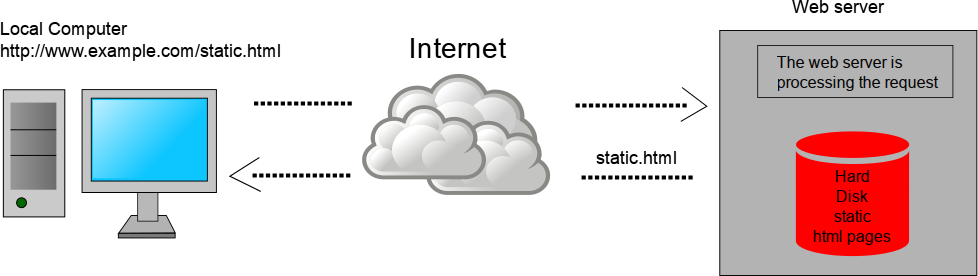
\includegraphics[scale=0.5]{Scheme_static_page_en.png}
\caption{Static web page: is delivered to the user exactly as stored.}
\label{Scheme_static_page_en}
\end{figure}


Consequently a static web page displays the same information for all users, from all contexts, subject to modern capabilities of a web server to negotiate content-type or language of the document where such versions are available and the server is configured to do so.

Static web pages are often HTML documents stored as files in the file system and made available by the web server over HTTP (nevertheless URLs ending with ".html" are not always static). However, loose interpretations of the term could include web pages stored in a database, and could even include pages formatted using a template and served through an application server, as long as the page served is unchanging and presented essentially as stored.

Static web pages are suitable for the contents that never or rarely need to be updated. However, maintaining large numbers of static pages as files can be impractical without automated tools. Any personalization or interactivity has to run client-side, which is restricting.







\chapter{Dynamic web page}




A dynamic web page\cite{dynamic_web_page} is a web page with rendered web content that varies based on parameters provided by a user or a computer program presenting content that has been customized or actualized for each individual viewing or rendition or that continually updates information as the page is displayed to the user.

\begin{figure}[!h]
\centering
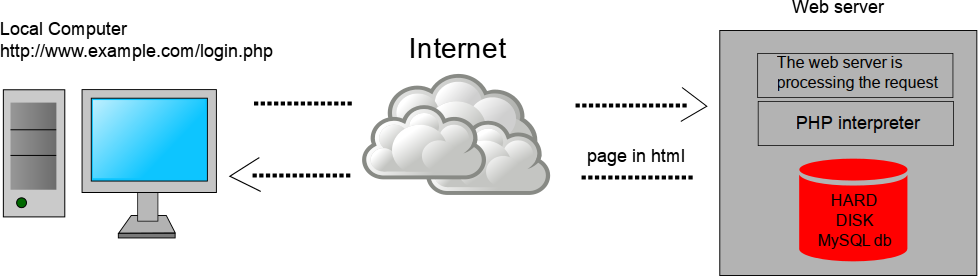
\includegraphics[scale=0.5]{Scheme_dynamic_page_en.png}
\caption{Dynamic web page: example of server-side scripting (PHP and MySQL).}
\label{Scheme_dynamic_page_en}
\end{figure}



\section{Client-side scripting}

Client-side scripting is changing interface behaviors within a specific web page in response to mouse or keyboard actions, or at specified timing events. In this case, the dynamic behavior occurs within the presentation. The Client-side content is generated on the user's local computer system.

Such web pages use presentation technology called rich interfaced pages. Client-side scripting languages like JavaScript or ActionScript, used for Dynamic HTML (DHTML) and Flash technologies respectively, are frequently used to orchestrate media types (sound, animations, changing text, etc.) of the presentation. The scripting also allows use of remote scripting, a technique by which the DHTML page requests additional information from a server, using a hidden frame, XMLHttpRequests, or a Web service

The first "widespread used" version of JavaScript was in 1996 (with Netscape 3 and ECMAScript standard).










\section{Server-side scripting}


A program running on a web server (server-side scripting) is used to generate the web content on various web pages, manage user sessions, and control workflow. Server responses may be determined by such conditions as data in a posted HTML form, parameters in the URL, the type of browser being used, the passage of time, or a database or server state.

Such web pages are often created with the help of server-side languages such as ASP, ColdFusion, JavaScript Perl, PHP, Ruby, WebDNA and other languages. These server-side languages often use the Common Gateway Interface (CGI) to produce dynamic web pages. Two notable exceptions are ASP.NET, and JSP, which reuse CGI concepts in their APIs but actually dispatch all web requests into a shared virtual machine.

Dynamic web pages are often cached when there are few or no changes expected and the page is anticipated to receive considerable amount of web traffic that would create slow load times for the server if it had to generate the pages on the fly for each request.






\section{Combination}

Ajax is a web development technique for dynamically interchanging content which sends a request to the server for data. The server returns the requested data which is then formatted by a client side script. This technique can reduce server load time because the client does not request the entire webpage to be regenerated by the server's language parser; only the content that will change is transmitted. Google Maps is an example of a web application that uses Ajax techniques.

A Web client program (such as a web browser) can access data from many different servers, such as Gopher, FTP, NNTP (Usenet) or HTTP. The HTTP server was designed specifically for the Web, and employs a protocol (system of messages) that supports sending documents from the server to a browser, and that also support sending complex data from the client back to the server. There are several HTTP methods for doing this (in HTTP, method is a technical term for the way in which data are sent between a client browser and server).

All of the client and server components that collectively build dynamic web pages for one website are together called a web application. Web applications manage user interactions, state, security, and performance.






\section{History}


It is difficult to be precise about "dynamic web page beginnings" or chronology, because the precise concept makes sense only after the "widespread development of web pages": HTTP has been in use since 1990, HTML, as standard, since 1996. The web browsers explosion started with 1993's Mosaic. It is obvious, however, that the concept of dynamically driven websites predates the internet, and in fact HTML. For example, in 1990, before general public use of the internet, a dynamically driven remotely accessed menu system was implemented by Susan Biddlecomb, at the University of Southern California BBS on a 16 line TBBS system with TDBS add-on.database.

Execusite introduced the first dynamic website solution for the professional marketplace in June 1997. Execusite was acquired by Website Pros (now Web.com) in January 2000. During the bust cycle of the Dot-com bubble, the original Execusite founders bought back the company from Website Pros (December 2000). Execusite was later acquired by Wolters-Kluwer in December 2001 and was re-branded as CCH Site Builder.





\chapter{Web Application}

In computing, a web-based application\cite{web_application} is any application that uses a web browser as a client. The term may also mean a computer software application that is coded in a browser-supported programming language (such as JavaScript, combined with a browser-rendered markup language like HTML) and reliant on a common web browser to render the application executable.


Web applications are popular due to the ubiquity of web browsers, and the convenience of using a web browser as a client, sometimes called a thin client. The ability to update and maintain web applications without distributing and installing software on potentially thousands of client computers is a key reason for their popularity, as is the inherent support for cross-platform compatibility. Common web applications include webmail, online retail sales, online auctions, wikis and many other functions.

网络应用程序(简称 Webapp)是一种使用网页浏览器在互联网或企业内部网上操作的应用软件。是一种以网页语言(例如HTML、JavaScript、Java等编程语言)撰写的应用程序,需要通过浏览器来运行。

网络应用程序风行的原因之一,是因为可以直接在各种电脑平台上运行,不需要事先安装或定期升级等程序。常见的网页应用程序有Webmail、网络商店、网络拍卖、wiki、网络论坛、博客、网络游戏等许多应用。

\begin{compactitem}
\item 网络应用程序不需要任何复杂的“展开”过程,用户所需要的只是一个适用的浏览器;
\item 网络应用程序通常耗费很少的用户硬盘空间,或者一点都不耗费;
\item 它们不需要更新,因为所有新的特性都在服务器上执行,从而自动传达到用户端;
\item 网络应用程序和服务器端的网络产品都很容易结合,如email功能和搜索功能;
\item 因为它们在网络浏览器窗口中运行,所以大多数情况下它们是通过跨平台使用的 (例如Windows,Mac,Linux等等)
\end{compactitem}



\section{History}


In earlier computing models, e.g. in client-server, the load for the application was shared between code on the server and code installed on each client locally. In other words, an application had its own client program which served as its user interface and had to be separately installed on each user's personal computer. An upgrade to the server-side code of the application would typically also require an upgrade to the client-side code installed on each user workstation, adding to the support cost and decreasing productivity.

In contrast, web applications use web documents written in a standard format such as HTML and JavaScript, which are supported by a variety of web browsers. Web applications can be considered as a specific variant of client-server software where the client software is downloaded to the client machine when visiting the relevant web page, using standard procedures such as HTTP. Client web software updates may happen each time the web page is visited. During the session, the web browser interprets and displays the pages, and acts as the universal client [3] for any web application.

In the early days of the Web each individual web page was delivered to the client as a static document, but the sequence of pages could provide an interactive experience, as user input is returned through web form elements embedded in the page markup.

In 1995 Netscape introduced a client-side scripting language called JavaScript allowing programmers to add some dynamic elements to the user interface that ran on the client side. So instead of sending data to the server in order to generate an entire web page, the embedded scripts of the downloaded page can perform various tasks such as input validation or showing/hiding parts of the page.

In 1996, Macromedia introduced Flash, a vector animation player that could be added to browsers as a plug-in to embed animations on the web pages. It allowed the use of a scripting language to program interactions on the client side with no need to communicate with the server.

In 1999, the "web application" concept was introduced in the Java language in the Servlet Specification version 2.2. [2.1?].[4][5] At that time both JavaScript and XML had already been developed, but Ajax had still not yet been coined and the XMLHttpRequest object had only been recently introduced on Internet Explorer 5 as an ActiveX object.[6]

In 2005, the term Ajax was coined, and applications like Gmail started to make their client sides more and more interactive. A web page script is able to contact the server for storing/retrieving data without downloading an entire web page.

In 2011, HTML5 was finalized, which provides graphic and multimedia capabilities without the need of client side plugins. HTML5 also enriched the semantic content of documents. The APIs and document object model (DOM) are no longer afterthoughts, but are fundamental parts of the HTML5 specification. WebGL API paved the way for advanced 3D graphics based on HTML5 canvas and JavaScript language. These have significant importance in creating truly platform and browser independent rich web applications.






\section{Interface}

Through Java, JavaScript, DHTML, Flash, Silverlight and other technologies, application-specific methods such as drawing on the screen, playing audio, and access to the keyboard and mouse are all possible. Many services have worked to combine all of these into a more familiar interface that adopts the appearance of an operating system. General purpose techniques such as drag and drop are also supported by these technologies. Web developers often use client-side scripting to add functionality, especially to create an interactive experience that does not require page reloading. Recently, technologies have been developed to coordinate client-side scripting with server-side technologies such as PHP. Ajax, a web development technique using a combination of various technologies, is an example of technology which creates a more interactive experience.








\section{Structure}

Applications are usually broken into logical chunks called "tiers", where every tier is assigned a role. Traditional applications consist only of 1 tier, which resides on the client machine, but web applications lend themselves to an n-tiered approach by nature. Though many variations are possible, the most common structure is the three-tiered application.[7] In its most common form, the three tiers are called presentation, application and storage, in this order. A web browser is the first tier (presentation), an engine using some dynamic Web content technology (such as ASP, ASP.NET, CGI, ColdFusion, JSP/Java, PHP, Perl, Python, Ruby on Rails or Struts2) is the middle tier (application logic), and a database is the third tier (storage). The web browser sends requests to the middle tier, which services them by making queries and updates against the database and generates a user interface.

For more complex applications, a 3-tier solution may fall short, and it may be beneficial to use an n-tiered approach, where the greatest benefit is breaking the business logic, which resides on the application tier, into a more fine-grained model. Another benefit may be adding an integration tier that separates the data tier from the rest of tiers by providing an easy-to-use interface to access the data. For example, the client data would be accessed by calling a "list\_clients()" function instead of making an SQL query directly against the client table on the database. This allows the underlying database to be replaced without making any change to the other tiers.


There are some who view a web application as a two-tier architecture. This can be a "smart" client that performs all the work and queries a "dumb" server, or a "dumb" client that relies on a "smart" server. The client would handle the presentation tier, the server would have the database (storage tier), and the business logic (application tier) would be on one of them or on both. While this increases the scalability of the applications and separates the display and the database, it still doesn't allow for true specialization of layers, so most applications will outgrow this model.






\section{Business use}


An emerging strategy for application software companies is to provide web access to software previously distributed as local applications. Depending on the type of application, it may require the development of an entirely different browser-based interface, or merely adapting an existing application to use different presentation technology. These programs allow the user to pay a monthly or yearly fee for use of a software application without having to install it on a local hard drive. A company which follows this strategy is known as an application service provider (ASP), and ASPs are currently receiving much attention in the software industry.

Security breaches on these kinds of applications are a major concern because it can involve both enterprise information and private customer data. Protecting these assets is an important part of any web application and there are some key operational areas that must be included in the development process.[8] This includes processes for authentication, authorization, asset handling, input, and logging and auditing. Building security into the applications from the beginning can be more effective and less disruptive in the long run.

In cloud computing model web applications are software as a service (SaaS). There are business applications provided as SaaS for enterprises for fixed or usage dependent fee. Other web applications are offered free of charge, often generating income from advertisements shown in web application interface.

Many businesses are enabled by open source web applications such as e-commerce software that facilitates easily creating an online retail store. Most businesses today do not need to buy data center hardware such as servers because they are affordably rented on a short term basis from a plethora of hosting companies that provide turnkey implementations of web applications. It is common for hosting providers to also offer packages of hardware and all necessary software to support the business needs of a company. Innovations in all aspects of web applications are providing tremendous economic value by increasing competition by reducing barriers to entry for new companies.





\section{Writing web applications}


Writing of web applications is often simplified by open source software such as Django, Ruby on Rails or Symfony called web application frameworks. These frameworks facilitate rapid application development by allowing a development team to focus on the parts of their application which are unique to their goals without having to resolve common development issues such as user management.[9] While many of these frameworks are open source, this is by no means a requirement.

The use of web application frameworks can often reduce the number of errors in a program, both by making the code simpler, and by allowing one team to concentrate on the framework while another focuses on a specified use case. In applications which are exposed to constant hacking attempts on the Internet, security-related problems can be caused by errors in the program. Frameworks can also promote the use of best practices[10] such as GET after POST.

In addition, there is potential for the development of applications on Internet operating systems, although currently there are not many viable platforms that fit this model.




\section{Applications}


Examples of browser applications are simple office software (word processors, online spreadsheets, and presentation tools), but can also include more advanced applications such as project management, computer-aided design, video editing and point-of-sale.






\section{Benefits}

\begin{compactitem}
\item Web applications do not require any complex "roll out" procedure to deploy in large organizations. A compatible web browser is all that is needed;
\item Browser applications typically require little or no disk space on the client;
\item They require no upgrade procedure since all new features are implemented on the server and automatically delivered to the users;
\item Web applications integrate easily into other server-side web procedures, such as email and searching.
\item They also provide cross-platform compatibility in most cases (i.e., Windows, Mac, Linux, etc.) because they operate within a web browser window.
\item With the advent of HTML5, programmers can create richly interactive environments natively within browsers. Included in the list of new features are native audio, video and animations, as well as improved error handling.
\item Modern web applications support greater interactivity and greatly improved usability through technologies such as AJAX that efficiently exchange data between the browser and the server.
\item Web applications allow for easier introduction of new user devices (e.g. smartphones, tablets) because they have built-in browsers.
\end{compactitem}




\section{Drawbacks}

\begin{compactitem}
\item In practice, web interfaces, compared to thick clients, typically force significant sacrifice to user experience and basic usability.
\item Web applications absolutely require compatible web browsers. If a browser vendor decides not to implement a certain feature, or abandons a particular platform or operating system version, this may affect a huge number of users;
\item Standards compliance is an issue with any non-typical office document creator, which causes problems when file sharing and collaboration becomes critical;
\item Browser applications rely on application files accessed on remote servers through the Internet. Therefore, when connection is interrupted, the application is no longer usable. However, if it uses HTML5 API's such as Offline Web application caching,[11] it can be downloaded and installed locally, for offline use. Google Gears, although no longer in active development, is a good example of a third party plugin for web browsers that provides additional functionality for creating web applications;
\item Since many web applications are not open source, there is also a loss of flexibility, making users dependent on third-party servers, not allowing customizations on the software and preventing users from running applications offline (in most cases). However, if licensed, proprietary software can be customized and run on the preferred server of the rights owner;
\item They depend entirely on the availability of the server delivering the application. If a company goes bankrupt and the server is shut down, the users have little recourse. Traditional installed software keeps functioning even after the demise of the company that produced it (though there will be no updates or customer service);
\item Likewise, the company has much greater control over the software and functionality. They can roll out new features whenever they wish, even if the users would like to wait until the bugs have been worked out before upgrading. The option of simply skipping a weak software version is often not available. The company can foist unwanted features on the users or cut costs by reducing bandwidth. Of course, companies will try to keep the good will of their customers, but the users of web applications have fewer options in such cases unless a competitor steps in and offers a better product and easy migration;
\item The company can theoretically track anything the users do. This can cause privacy problems.
\item According to Jonathan Zittrain, the online applications like Facebook and Google Apps have made the Internet become far more proprietary than early versions of Microsoft Windows.
\end{compactitem}

\begin{compactitem}
\item 网络应用程序强调浏览器的适用性。如果浏览器方没有提供特定的功能,或者弃用特定的平台或操作系统版本(导致不适用),就会影响大量用户;
\item 网络应用依靠互联网远程服务器端的应用文件。因此,当连接出问题时,应用将不能正常使用。但是,如果使用HTML5 API,这些应用就可以被下载安装而可离线使用。Google Gears,就是一个好例子;
\item 许多网络应用程序不是开源的,只能依赖第三方提供的服务,因此不能针对用户定制化、个性化,而且大多数情况下用户不能离线使用,因而损失了很多灵活性;
\item 它们完全依赖应用服务商的可及性。如果公司倒闭,服务器停止使用,用户也无法追索以前的资料。对比而看,即使软件制造商倒闭了,传统的安装软件也可以继续运行,尽管不能再更新或有其他用户服务;
\item 相似地,提供方公司对软件和其功能有了更大的控制权。只要他们愿意就能为软件添加新特性,即使用户想等bugs先被解决再更新。跳过较差的软件版本也不可能了。公司可以强加不受欢迎的特性给用户,也可以随意减少带宽来削减开支。当然,公司会尽量地讨用户欢喜——只在有竞争者提供更好的服务与方便的转接性的情况下。否则用户别无选择,只能默默承受;
\item 公司理论上可以检索任何的用户行为。这有可能引起隐私安全问题。
\end{compactitem}


\clearpage

\bibliographystyle{plainnat}
\bibliography{webdevelopment}


































\part{Specification}



\chapter{Overview}




\chapter{Directory}


项目目录结构规范\footnote{directory_spec}的设计目标是项目开发的目录结构保持一致,使容易理解并方便构建与管理。


\begin{compactitem}
\item 项目包含但不限于业务项目和包项目。
\item \texttt{\$\{root\}}表示项目的根目录。
\end{compactitem}


资源分成两大类,分别是源代码资源和内容资源。

\begin{compactenum}
\item 源代码资源:开发者编写的源代码,包括js、html、css、template等。
\item 内容资源:希望作为内容提供给访问者的资源,包括图片、字体、flash、pdf等。
\end{compactenum}

\section{Naming}


目录命名原则要求简洁,不允许使用复数。

习惯性缩写的单词 必须(MUST) 采用容易理解的缩写。例如,源代码目录使用src,不使用source。

\begin{compactitem}
\item img(图片),不允许(MUST NOT) 使用image、images、imgs等。
\item js(javascript脚本),不允许(MUST NOT) 使用script、scripts等。
\item css(样式表),不允许(MUST NOT) 使用style、styles等。
\item swf(flash),不允许(MUST NOT) 使用flash等。
\item src(源文件目录),不允许(MUST NOT) 使用source等。
\item dep(引入的第三方依赖包目录),不允许(MUST NOT) 使用lib、library、dependency等。
\end{compactitem}

不允许(MUST NOT) 使用复数形式。例如,imgs、docs是不被允许的。

\section{Structure}

在\$\{root\}下,目录结构必须(MUST) 按照职能进行划分, 不允许(MUST NOT) 将资源类型或业务逻辑划分的目录直接置于\$\{root\}下。

常用的目录有src、doc、dep、test等。

\begin{lstlisting}[language=bash]
${root}/
    src/
    test/
    doc/
    dep/
    ...
\end{lstlisting}


业务项目的\$\{root\}目录结构划分遵循\$\{root\}目录结构划分。


从程序结构的角度来看,必须合理设计项目的目录结构。例如,支持文件和引用文件不能保存在公众可以公开访问的目录中,用户信息必须存储在数据库中。

在项目开发过程中的第一步就是设计良好的项目目录结构。例如,下面是一个PHP项目目录结构的初级设计。

\begin{lstlisting}[language=bash]
${root}/
    pub/
    lib/
    tpl/
\end{lstlisting}


\begin{compactitem}
\item pub/保存所有可以公开访问的页面;
\item lib/保存可以被其他文件调用的引用文件;
\item tpl/保存页面显示文件。
\end{compactitem}

在实际网站中,Web服务器应该只允许访客访问pub/目录下的文件(例如样式表、脚本和图片等),其他文件必须保存在公共目录之外的目录中。


\begin{lstlisting}[language=bash]
${root}/
    pub/
        img/
        css/
        js/
    lib/
    tpl/
\end{lstlisting}


Web服务器的根目录是一个特殊目录,应该通过httpd.conf或URL重写等指向指定的主页。


\begin{lstlisting}[language=bash]
# cat /etc/httpd/conf/httpd.conf
#
# DirectoryIndex: sets the file that Apache will serve if a directory
# is requested.
#
<IfModule dir_module>
    DirectoryIndex index.html
</IfModule>
\end{lstlisting}

除此之外,还需要创建其他的目录来提供与项目开发过程相关的资源,并且保持代码结构的清晰性。


\begin{lstlisting}[language=bash]
${root}/
    pub/
        img/
        css/
        js/
    lib/
    tpl/
    sql/
    doc/
    test/
\end{lstlisting}


\begin{compactitem}
\item sql/保存MySQL文件等;
\item doc/保存帮助文档和开发笔记等;
\item test/保存发烟测试和单元测试代码等。
\end{compactitem}

最后也是最基础的,只要页面需要被用户访问,那么它就应该被放置到可以公开访问的目录中,至于其执行过程则由Web服务器和应用程序本身来负责。


\begin{lstlisting}[language=bash]

\end{lstlisting}




\begin{lstlisting}[language=bash]

\end{lstlisting}




\begin{lstlisting}[language=bash]

\end{lstlisting}





\section{Code}

业务项目可以(SHOULD) 为项目起一个代号名称,代号名称 必须(MUST) 为一个单词,不宜过长。例如,北斗的项目代号为triones,哥伦布的项目代号为clb。

项目代号应该有利于区分不同项目,为未来项目之间的重用留下扩展的后路。


在项目开发时,通常会使用如下加载器配置,将项目代号指向src。


\begin{lstlisting}[language=bash]
{
    baseUrl: '${docroot}',
    paths: {
        'triones': 'src'
    }
}
\end{lstlisting}

业务项目的src目录内,绝大多数情况 应当(SHOULD) 根据业务逻辑划分目录结构。划分出的子目录(比如例子中的biz1)称为业务目录。


src下 必须(MUST) 只包含业务目录与common目录。业务公共资源 必须(MUST) 命名为common。common目录作为业务公共资源的目录,也视如业务目录。




\begin{lstlisting}[language=bash]
${root}/
    src/
        common/
        biz1/
            subbiz1/
            subbiz2/
        biz2/
\end{lstlisting}

较小规模的业务项目(如投放端),src目录允许视如业务目录,直接按照业务目录划分原则划分目录结构。


\begin{lstlisting}[language=bash]
${root}/
    src/
        foo.js
\end{lstlisting}


\section{Database}


在设计项目目录结构的同时也需要根据需求来设计数据库结构。

项目(例如网站)需要从用户处收集的信息和项目本身所能提供的服务相关,而且这些信息又会反过来影响数据库设计中的表结构等。




\section{Principle}

\begin{compactenum}
\item JS资源:不允许(MUST NOT) 按资源类型划分目录, 必须(MUST) 按业务逻辑划分目录。JS资源应直接置于业务目录下。即:业务目录下不允许出现js目录。
\item 除JS资源外的源文件资源,当资源数量较多时,为方便管理, 允许(SHOULD) 按资源类型划分目录。即:业务目录下允许出现css、tpl目录。
\item 内容资源:允许(SHOULD) 按资源类型划分目录。即:业务目录下允许出现img、swf、font目录。
\item 业务目录中,如果文件太多不好管理,需要划分子目录时,也 必须(MUST) 继续遵守根据业务逻辑划分的原则,划分子业务。如:下面例子中的subbiz1。
\end{compactenum}


\subsection{Biz}


通常,对于一个业务目录, 鼓励(SHOULD) 将业务相关的源文件资源都直接置于业务目录下。


\begin{lstlisting}[language=bash]
biz1/
    img/
        add_button.png
    add.js
    add.tpl.html
    add.css
\end{lstlisting}

业务目录下源文件资源数量较多时,我们第一直觉应该是:是否业务划分不够细?是否应该划分子业务,建立子业务目录?



\begin{lstlisting}[language=bash]
biz2/
    subbiz1/
        list.js
        list.tpl.html
        list.css
    subbiz2/
\end{lstlisting}

遇到确实是一个业务整体,无法划分子业务时, 允许(MAY) 将非JS资源按资源类型划分目录进行管理。


\begin{lstlisting}[language=bash]
biz1/
    css/
        add.css
        edit.css
        remove.css
        img/
            add_button.png
    tpl/
        add.html
        edit.html
        remove.html
    add.js
    edit.js
    remove.js
\end{lstlisting}

业务项目目录划分示例


\begin{lstlisting}[language=bash]
${root}/
    src/
        common/
            img/
                sprites.png
                logo.png
            conf.js
            layout.css
        biz1/
            img/
                add_button.png
            add.js
            add.tpl.html
            add.less
        biz2/
            subbiz1/
                list.js
                list.tpl.html
                list.css
            subbiz2/
    dep/
        er/
            src/
            test/
        esui/
            src/
            test/
    test/
    doc/
    index.html
    main.html
    ......
\end{lstlisting}


common目录为业务公共目录,用于存放业务项目的业务公共文件。所以,根据业务逻辑划分目录结构时,业务逻辑命名 不允许(MUST NOT) 为common。

biz下面不能有资源类型目录,否则如果在biz下继续划分资源目录,代码的结构可能如下:



\begin{lstlisting}[language=bash]
${root}/
    src/
        biz1/
            js/
                list.js
\end{lstlisting}

当我们需要使用list.js的时候,必须写如下的代码:\texttt{require("../biz1/js/list")},但是从逻辑上说,更合理的写法应该是\texttt{require("../biz1/list")},因此不推荐在biz下面对源代码资源划分目录。


\subsection{Package}


包项目的\$\{root\}目录结构划分遵循\$\{root\}目录结构划分。

包是实现某个独立功能,有复用价值的代码集。按照通常的理解,一个包项目不应该特别复杂,所以包可视如一个不太复杂的业务,其src下的划分原则与业务项目的业务目录划分原则保持一致。




\begin{lstlisting}[language=bash]
${root}/
    src/
        css/
            img/
                sprites.png
            table.css
            button.css
            select.css
        main.js
        Control.js
        InputControl.js
        Button.js
        Table.js
        Select.js
    test/
    doc/
    package.json
    ...
\end{lstlisting}


直接置于\$\{root\}下的目录称作一级目录。一级目录 必须(MUST) 具有某种职能属性。

除了下面列举的一些常见目录之外,\$\{root\}下也可以放置一些跟项目发布相关的文件,例如build.sh,build.xml,Makefile,Gruntfile等。

\begin{compactitem}
\item src

src目录用于存放开发时源文件,发布时 必须(MUST) 被删除。

\item dep

dep目录用于存放项目引入依赖的第三方包。该目录下的内容通过平台工具管理,项目开发人员 不允许(MUST NOT) 更改dep目录下第三方包的任何内容。

当项目需要修改引入的第三方代码时,第三方包应将源码直接置于\$\{root\}/src目录下,规则见该目录下的规定。


\item tool

tool目录用于存放开发时或构建阶段使用的工具。该目录在发布时 必须(MUST) 被删除。

\item test

test目录用于存放测试用例以及开发阶段的模拟数据。该目录在发布时 必须(MUST) 被删除。

\item doc

doc目录用于存放项目文档。项目文档可能是开发者维护的文档,也可能是通过工具生成的文档。

\item entry

entry目录用于存放项目的页面入口文件,通常是上线后可被直接访问的静态页面。

\item asset目录用于存放用于线上访问的静态资源。

通常构建工具会对src目录和dep目录下的资源进行分析、合并与压缩等,生成到asset目录下。所以该目录尽量避免手工管理。



\end{compactitem}


下面是一个构建工具生成后的asset目录示例:




\begin{lstlisting}[language=bash]
${root}/
    asset/
        js/
            loader.js
            build.js
        css/
            common.css
            img/
        tpl/
            build.tpl.html
        img/
        ...
\end{lstlisting}




RIA项目通常会包含较少的页面入口文件,常见的是main.html,这些文件 可以(SHOULD) 直接放在\$\{root\}目录下。




\begin{lstlisting}[language=bash]
${root}/
    src/
        common/
            conf.js
        card/
        gold/
        message/
    index.html
    main.html
    ......
\end{lstlisting}

多页面项目通常页面入口文件较多, 可以(SHOULD) 统一放在entry目录中,按业务逻辑命名。

\begin{lstlisting}[language=bash]
${root}/
    src/
        common/
            conf.js
        card/
        gold/
        message/
    entry/
        card.html
        gold.html
        message.html
        ......
\end{lstlisting}


项目在发布的时候,构建工具可以页面入口文件为入口进行分析和编译。

RIA项目经过构建工具编译后,目录结构可能如下:

\begin{lstlisting}[language=bash]
output/
    asset/
        js/
        css/
        tpl/
        img/
    index.html
    main.html
\end{lstlisting}

多页面项目经过构建工具编译后,目录结构可能如下:

\begin{lstlisting}[language=bash]
output/
    card/
        asset/
            js/
            css/
            img/
        index.html
    gold/
        asset/
            js/
            css/
            img/
        index.html
\end{lstlisting}


\subsection{Resource}


按资源类型命名的目录称作资源目录。资源目录 不允许(MUST NOT) 直接置于\$\{root\}下。


\begin{compactitem}
\item js目录可用于存放js资源文件(包含可编译成js的coffeescript等语言)。js文件后缀名 必须(MUST) 为.js,coffeescript文件后缀名 必须(MUST) 为.coffee。

js目录内 必须(MUST) 存放js资源文件,但js资源文件不一定(MAY NOT)存放于js目录下:

\begin{compactenum}
\item 对于src目录,js资源文件 不允许(MUST NOT) 存放于js目录下。
\item 对于asset目录,js资源文件 可以(SHOULD) 存放于js目录下,视构建行为决定。
\item 对于其他一级目录内,js资源文件 可以(SHOULD) 不存放于js目录下。
\end{compactenum}

\item css目录可用于存放css资源文件(包含less,sass等动态样式表语言)。css文件后缀名 必须(MUST) 为.css,less文件后缀名 必须(MUST) 为.less。

css目录内 必须(MUST) 存放css资源文件,但css资源文件不一定(MAY NOT)存放于css目录下:

\begin{compactenum}
\item 对于src目录,css资源文件 可以(SHOULD) 存放于业务目录下,也 可以(SHOULD) 存放于css目录下。
\item 对于asset目录,css资源文件 可以(SHOULD) 存放于css目录下,视构建行为决定。
\item 对于其他一级目录内,css资源文件 可以(SHOULD) 不存放于css目录下。
\end{compactenum}

\item img目录可用于存放图片资源文件。包括页面直接引用的图片与css引用图片。常见的图片资源有gif/jpg/png/svg/bmp等。

对于css引用的图片, 必须(MUST) 放在./img目录下,.代表当前css资源所在的目录。

对于页面直接引用的图片:



\begin{compactenum}
\item 被多页面引用的图片 应该(SHOULD) 放在\$\{root\}/src/common/img目录下。
\item 单一页面引用的图片 应该(SHOULD) 放在./img目录下,.代表当前页面所在的目录。
\end{compactenum}

\item tpl目录可用于存放template资源文件。template资源文件后缀名 可以(SHOULD) 为.html或.tpl。

通常,对于RIA系统,template资源文件采用.html后缀使其能够被xhr加载。

\item font目录可用于存放字体资源文件。常见的字体资源有tff/woff/svg等。


\item swf目录可用于存放flash资源文件。flash资源文件 不允许(MUST NOT) 置于img目录中。

\end{compactitem}




\begin{lstlisting}[language=bash]

\end{lstlisting}



\begin{lstlisting}[language=bash]

\end{lstlisting}




\begin{lstlisting}[language=bash]

\end{lstlisting}



\begin{lstlisting}[language=bash]

\end{lstlisting}




\begin{lstlisting}[language=bash]

\end{lstlisting}




\begin{lstlisting}[language=bash]

\end{lstlisting}



\begin{lstlisting}[language=bash]

\end{lstlisting}




\begin{lstlisting}[language=bash]

\end{lstlisting}



\begin{lstlisting}[language=bash]

\end{lstlisting}




\begin{lstlisting}[language=bash]

\end{lstlisting}




\begin{lstlisting}[language=bash]

\end{lstlisting}



\begin{lstlisting}[language=bash]

\end{lstlisting}




\begin{lstlisting}[language=bash]

\end{lstlisting}



\begin{lstlisting}[language=bash]

\end{lstlisting}




\begin{lstlisting}[language=bash]

\end{lstlisting}




\begin{lstlisting}[language=bash]

\end{lstlisting}



\begin{lstlisting}[language=bash]

\end{lstlisting}




\begin{lstlisting}[language=bash]

\end{lstlisting}



\begin{lstlisting}[language=bash]

\end{lstlisting}




\begin{lstlisting}[language=bash]

\end{lstlisting}




\begin{lstlisting}[language=bash]

\end{lstlisting}



\begin{lstlisting}[language=bash]

\end{lstlisting}




\begin{lstlisting}[language=bash]

\end{lstlisting}



\begin{lstlisting}[language=bash]

\end{lstlisting}




\begin{lstlisting}[language=bash]

\end{lstlisting}




\begin{lstlisting}[language=bash]

\end{lstlisting}



\begin{lstlisting}[language=bash]

\end{lstlisting}




\begin{lstlisting}[language=bash]

\end{lstlisting}



\begin{lstlisting}[language=bash]

\end{lstlisting}




\begin{lstlisting}[language=bash]

\end{lstlisting}




\begin{lstlisting}[language=bash]

\end{lstlisting}



\begin{lstlisting}[language=bash]

\end{lstlisting}




\begin{lstlisting}[language=bash]

\end{lstlisting}



\begin{lstlisting}[language=bash]

\end{lstlisting}




\begin{lstlisting}[language=bash]

\end{lstlisting}




\begin{lstlisting}[language=bash]

\end{lstlisting}



\begin{lstlisting}[language=bash]

\end{lstlisting}




\begin{lstlisting}[language=bash]

\end{lstlisting}



\begin{lstlisting}[language=bash]

\end{lstlisting}




\begin{lstlisting}[language=bash]

\end{lstlisting}




\begin{lstlisting}[language=bash]

\end{lstlisting}



\begin{lstlisting}[language=bash]

\end{lstlisting}




\begin{lstlisting}[language=bash]

\end{lstlisting}



\begin{lstlisting}[language=bash]

\end{lstlisting}




\begin{lstlisting}[language=bash]

\end{lstlisting}




\begin{lstlisting}[language=bash]

\end{lstlisting}

\part{Server}


\chapter{Overview}


一般来说,网络中的服务器对外提供服务,可以通过 Intranet 对内网提供服务,也可以通过 Internet 对外提供服务。

原始的通信网络中的电话和传真等设备的地位是对等的,但是用户和服务器的地位是不对等的,二者之间始终是发送请求和返回响应的关系。

P2P(peer-to-peer)对等网络中通过去中心化来实现了节点之间直接连接,并完成各自的连接认证、传输加密、数据压缩和数据校验等,因此P2P已经不同于客户端-服务器模型。

\begin{compactitem}
\item 对等网络要求通信双方必须同时在线;
\item 客户端-服务器模型要求服务器必须始终在线。
\end{compactitem}

软件服务器可以是管理资源并为用户提供服务的计算机软件,例如文件服务器(能使用户在其它计算机访问文件)、数据库服务器和应用程序服务器等,运行相关服务器软件的计算机就被称为硬件服务器,或主机(Host)。

最初,服务器通常是指具有较高计算能力,能够提供给多个用户使用的计算机,服务器软件工作在客户端-服务器或浏览器-服务器等模式下。


\begin{compactitem}
\item 文件服务器(File Server)或网络存储设备(Network Attached Storage);
\item 数据库服务器(Database Server),例如Oracle、MySQL、PostgreSQL和SQL Server 等;
\item 邮件服务器(Mail Server), 例如Sendmail、Postfix、Microsoft Exchange和Lotus Domino等;
\item 网页服务器(Web Server),例如httpd、IIS 和 nginx 等;
\item FTP 服务器(FTP Server),例如 vsftpd 和 Serv-U 等;
\item 域名服务器(DNS Server),例如BIND;
\item 应用程序服务器(Application Server),例如WebLogic、JBoss和GlassFish等;
\item 代理服务器(Proxy Server),例如Squid等。
\end{compactitem}


文件服务器可以为其他客户端提供文件检索和存储,通常具备某些特定的功能(例如磁盘镜像、多个网络接口等),后来文件服务器逐渐进化成带有 RAID 存储子系统和其他高可用特性的高性能存储系统。


在讨论主从式架构系统时,应用程序服务器区别于数据库服务器和文件服务器等,通常可以认为是运行Web应用程序的Web服务器。

具体来说,应用程序服务器是一种提供应用程序运行的环境的软件框架,可以为应用程序提供安全、数据、事务支持、负载平衡和分布式系统管理等服务。


网页服务器(Web server)可能是指用于网站的主机,也可能是指类似 httpd 的软件,运行在主机上并管理网页组件和回应网页浏览器的请求。例如,Redhat JBoss、Apache Tomcat和Oracle WebLogic等可以运行JSP的Web服务器都可以被认为是应用程序服务器。

每一个网页服务器至少会运行一个网页服务器程序,因此网页服务器也称为Web服务器,现在的Web服务器一般是指可以通过 HTTP 协议或 HTTPS 协议将 HTML 代码发送回客户端的主机,或者提供网页服务的服务器软件。

随着摩尔定律对于计算机硬件的影响和计算机软件的进化,服务器开始把越来越多的计算机任务放到客户端(例如Web浏览器)执行,这样服务器就可以专注于高性能计算和分布式计算等领域。



\section{C/S}



客户端-服务器(Client/Server)结构是一种把客户端与服务器区分开来的网络架构。例如,WWW就是客户端/服务器结构,服务器存储WWW资源,并响应客户端的请求。

\begin{compactitem}
\item 接受请求并进行特化处理的计算机称为服务器,可能会返回响应;
\item 发送请求并接受响应的计算机称为客户机,可能会丢失连接。
\end{compactitem}


每一个客户端软件的实例都可以向一个服务器或应用程序服务器发出请求。例如,当用户在Wikipedia.org阅读文章时,其主机和网页浏览器就被当做一个客户端,Wikipedia.org的主机、数据库和应用程序就被当做服务器。当网页浏览器向Wikipedia.org请求一个指定的文章时,Wikipedia.org的服务器从数据库中找出所有该文章需要的信息,并组合成一个网页,然后再发送回客户端的浏览器。

具体来说,服务端的特征可以包括:

\begin{compactitem}
\item 被动的角色(从)。
\item 等待来自用户端的请求。
\item 处理要求并传回结果。
\end{compactitem}

客户端的特征包括:

\begin{compactitem}
\item 主动的角色(主)。
\item 发送请求。
\item 等待直到收到回应,或退出。
\end{compactitem}

服务器可以是有状态或者无状态的。其中,无状态的服务器不会保留任何两个请求之间的信息,有状态服务器会记住请求之间的信息。

服务器与客户端之间的状态信息的作用域可以是全局的或者某个事务(session)的。例如,静态 HTML 页面服务器是一个无状态服务器的例子,而 Tomcat 是一个有状态服务器。



服务器端与客户端的交互可以使用循序图描述,循序图是 UML 中的一个标准。

点对点(peer-to-peer)架构不同于 C/S 架构,P2P网络上的每个使用端或程序的实体都拥有相同的等级,同时扮演客户端与服务器端的角色。





\section{B/S}

HTTP 是一个客户端终端和服务器端请求和应答的标准,其中定义了信息的传输格式化、如何被传输以及在各种命令下服务器和浏览器所采取的响应。

用户通过HTTP或者HTTPS协议请求的资源由URI(Uniform Resource Identifiers,统一资源标识符)来标识。

Web 服务器程序可以从网络接受 HTTP 请求并进行处理,然后提供 HTTP 回复给请求者,不过根据Web服务器的类型不同,其内部操作也有很大差别。

\begin{compactitem}
\item 客户端浏览器、网络爬虫或者其它的工具发起HTTP请求到服务器上指定端口(默认端口为 80),可以将客户端看作是用户的代理程序(user agent)。
\item HTTP 回复一般包含一个 HTML 文件,也可以包含纯文本文件、图像或其他类型的文件。
\end{compactitem}




一般来说,文件(例如HTML、文本或图像等)都存储在 Web 服务器的本地文件系统中,并且 URL(Uniform Resource Locator) 和本地文件名都有对应的组织结构,因此服务器可以简单的把 URL 映射到本地文件系统中,并且可以指定一个本地路径名为根目录。

Web 服务器上可以用来存储一些资源(例如 HTML 文件和图像),因此也可以将 Web 服务器称为源服务器(origin server),而且在用户代理和源服务器中间可能存在多个“中间层”(例如代理、网关或者隧道(tunnel))。

客户端访问静态Web服务器(或静态网站)时,根据用户的选择将会返回相应的静态页面。例如,在 example.test.com 服务器上安装了服务器软件,并把服务器软件的根目录指定为/home/public/web/,当一个浏览者输入 http://example.test.com/lips/index.html时,就可以指定example.test.com的服务器软件读取/home/public/web/lips/index.html 文件。



默认情况下,Web 服务器的根目录为/var/www/html 或/src/www,例如 CentOS 默认的网站根目录为/var/www/html。如果需要自定义网站根目录,可以在修改 httpd.conf 中的DocumentRoot 参数,而且务必开放权限让 Web 服务器(例如 httpd、Nginix、Lightttpd)的用户可以浏览网站根目录。




Web服务器也可以提供动态内容,而且动态内容可以是该服务器本身提供的功能或者可借助外挂模块实现的功能。例如,通过动态网站技术生成的网页都称为动态网页,服务器端程序根据客户端请求来返回相应的结果。

动态网站技术可以通过查询字符串等参数并配合HTTP方法来实现更多的功能,而且动态网页并不是独立保存在服务器上的网页文件,只有当用户向服务器发送请求时才会组合相关组件并返回一个完整的网页。

\begin{compactitem}
\item 用户注册
\item 用户登录
\item 在线调查
\item 用户管理
\item 订单管理
\end{compactitem}

用户可以使用静态语言或动态语言来创建网站,动态语言不需要任何预先处理就可以快速反馈结果,而且动态语言引擎可以作为Web服务器的一部分来运行代码,不需要调用外部程序,这样Web服务器就不需要承担任何额外的负担。

例如,PHP应用程序可以检查请求的URI或其他信息来确定需要执行的操作,并且根据需要来从数据库中检索信息,然后将这些信息通过HTML组合成相应网页,最后将结果返回给客户端浏览器。当用户在浏览器中持续操作时,每次请求都会触发上述完整的过程被重复执行,并且当多个用户访问动态网站时,Web服务器会进行并发处理。

\begin{center}
HTML+运算结果=最终网页
\end{center}

Web浏览器实现的动态处理功能可以让浏览器在处理HTML或XML的同时显示图像或动画等,而且浏览器可以处理并执行从Web服务器获得的脚本或其他多媒体信息。

默认情况下,Web浏览器除了发送请求、接收响应和渲染输出之外功能有限,不过通过其内置的脚本引擎(例如Google V8引擎)或第三方插件等可以实现和操作系统相应的动态处理功能。



\begin{compactitem}
\item Adobe Flash Player可以让浏览器播放flash动画;
\item Apple Quicktime Player可以让浏览器播放mov视频;
\item Mozilla PDF.js可以让浏览器在线打开PDF文档。
\end{compactitem}


\chapter{LAMP}


Linux、Apache、MySQL和PHP等开放源代码程序本身并不是专门设计成同其他程序协同工作的,但是由于它们的廉价和普遍,LAMP组合才开始流行并被大多数Linux发行版本进行了捆绑发行。


在LAMP中的软件被合理地使用时,它们地表现类似一个具有活力的“解决方案包”(Solution Packages)。

最初,LAMP的脚本组件中包括了使用Perl实现地CGI Web接口,可以允许网页浏览器的用户在服务器上执行一个程序,并且和接受静态的内容一样接受动态的内容。

脚本语言(例如Perl、PHP和Python等)可以有效地操作文本流,因此被开发者引入来创建Web服务器上的外部程序。

从RHEL/CentOS 7开始已经不再內置MySQL并改用MariaDB,不过MariaDB和MySQL的使用方式相同,原来的MySQL数据库也可以直接升級使用。


\section{Apache}

\subsection{Compile}

下载源代码(httpd-2.4.16),并以默认配置来编译安装Apache。

\begin{lstlisting}[language=bash]
$ cd ~
$ mkdir src
$ cd src
$ wget http://mirrors.aliyun.com/apache/httpd/httpd-2.4.16.tar.gz
--2015-08-11 22:47:46--  http://mirrors.aliyun.com/apache/httpd/httpd-2.4.16.tar.gz
Resolving mirrors.aliyun.com (mirrors.aliyun.com)... 115.28.122.210, 112.124.140.210
Connecting to mirrors.aliyun.com (mirrors.aliyun.com)|115.28.122.210|:80... connected.
HTTP request sent, awaiting response... 200 OK
Length: 6899517 (6.6M) [application/octet-stream]
Saving to: ‘httpd-2.4.16.tar.gz’

httpd-2.4.16.tar.gz  100%[================>]  6.58M  1.00MB/s  in 7.3s   

2015-08-11 22:47:53 (918 KB/s) -‘httpd-2.4.16.tar.gz’ saved [6899517/6899517]
$ tar zxvf httpd-2.4.16.tar.gz
httpd-2.4.16/
httpd-2.4.16/.deps
httpd-2.4.16/.gdbinit
httpd-2.4.16/ABOUT_APACHE
httpd-2.4.16/acinclude.m4
httpd-2.4.16/ap.d
httpd-2.4.16/Apache-apr2.dsw
httpd-2.4.16/Apache.dsw
httpd-2.4.16/apache_probes.d
httpd-2.4.16/build/
httpd-2.4.16/BuildAll.dsp
httpd-2.4.16/BuildBin.dsp
httpd-2.4.16/buildconf
httpd-2.4.16/CHANGES
httpd-2.4.16/CMakeLists.txt
httpd-2.4.16/config.layout
httpd-2.4.16/configure
httpd-2.4.16/configure.in
httpd-2.4.16/docs/
httpd-2.4.16/emacs-style
httpd-2.4.16/httpd.dsp
httpd-2.4.16/httpd.spec
httpd-2.4.16/include/
httpd-2.4.16/INSTALL
httpd-2.4.16/InstallBin.dsp
httpd-2.4.16/LAYOUT
httpd-2.4.16/libhttpd.dsp
httpd-2.4.16/LICENSE
httpd-2.4.16/Makefile.in
httpd-2.4.16/Makefile.win
httpd-2.4.16/modules/
httpd-2.4.16/NOTICE
httpd-2.4.16/NWGNUmakefile
httpd-2.4.16/os/
httpd-2.4.16/README
httpd-2.4.16/README.cmake
httpd-2.4.16/README.platforms
httpd-2.4.16/ROADMAP
httpd-2.4.16/server/
httpd-2.4.16/srclib/
httpd-2.4.16/support/
httpd-2.4.16/test/
httpd-2.4.16/VERSIONING
httpd-2.4.16/test/.indent.pro
httpd-2.4.16/test/check_chunked
...
httpd-2.4.16/test/time-sem.c
httpd-2.4.16/support/.indent.pro
...
httpd-2.4.16/support/SHA1/README.sha1
httpd-2.4.16/srclib/Makefile.in
httpd-2.4.16/server/.indent.pro
...
httpd-2.4.16/server/mpm/event/mpm_default.h
httpd-2.4.16/os/.indent.pro
...
httpd-2.4.16/os/bs2000/os.h
httpd-2.4.16/modules/aaa/
...
httpd-2.4.16/modules/aaa/NWGNUmakefile
httpd-2.4.16/include/.indent.pro
...
httpd-2.4.16/include/util_xml.h
httpd-2.4.16/docs/cgi-examples/
...
httpd-2.4.16/docs/cgi-examples/test-cgi
httpd-2.4.16/build/aix/
...
httpd-2.4.16/build/aix/README
\end{lstlisting}

configure脚本

\begin{lstlisting}[language=bash]
$ cd src/httpd-2.4.16
$ ./configure
checking for chosen layout... Apache
checking for working mkdir -p... yes
checking for grep that handles long lines and -e... /usr/bin/grep
checking for egrep... /usr/bin/grep -E
checking build system type... x86_64-unknown-linux-gnu
checking host system type... x86_64-unknown-linux-gnu
checking target system type... x86_64-unknown-linux-gnu
configure: 
configure: Configuring Apache Portable Runtime library...
configure: 
checking for APR... no
configure: error: APR not found.  Please read the documentation.
\end{lstlisting}


\subsection{Dependence}


解决依赖关系

APR(Apache Portable Run-time Libraries)主要为上层的应用程序提供一个可以跨越多操作系统平台使用的底层支持接口库,其对于Tomcat最大的作用就是socket调度。例如,在慢速网络上(模拟Internet)将Tomcat线程数开到300以上,然后模拟大量的并发请求时没有APR,基本上300个线程很快就会用满,以后的请求就只好等待,在安装APR之后,并发的线程数量明显下降,从原来的300可能会马上下降到只有几十,这样新的请求会毫无阻塞的进来。

在早期的Apache版本中,应用程序本身必须能够处理各种具体操作系统平台的细节,并针对不同的平台调用不同的处理函数。随着Apache的进一步开发,Apache组织决定将这些通用的函数独立出来并发展成为一个新的项目,这样APR的开发就从Apache中独立出来,Apache仅仅是使用APR而已。

虽然在局域网进行本地测试时,高并发的情况也可以被很容易的处理,但是在真实的Internet环境下,页面处理时间只占0.1\%都不到,绝大部分时间都用来页面传输。如果不用APR,一个线程同一时间只能处理一个用户,势必会造成阻塞,所以生产环境下使用APR是非常必要的。

一般情况下,APR开发包很容易理解为仅仅是一个开发包,不过事实上并不是。目前,完整的APR实际上包含了三个开发包:apr、apr-util以及apr-iconv,每一个开发包分别独立开发,并拥有自己的版本。

\begin{lstlisting}[language=bash]
$ cd ~/src
$ wget http://mirrors.aliyun.com/apache/apr/apr-1.5.2.tar.gz
--2015-08-11 23:02:52--  http://mirrors.aliyun.com/apache/apr/apr-1.5.2.tar.gz
Resolving mirrors.aliyun.com (mirrors.aliyun.com)... 115.28.122.210, 112.124.140.210
Connecting to mirrors.aliyun.com (mirrors.aliyun.com)|115.28.122.210|:80... connected.
HTTP request sent, awaiting response... 200 OK
Length: 1031613 (1007K) [application/octet-stream]
Saving to: ‘apr-1.5.2.tar.gz’

apr-1.5.2.tar.gz  100%[======================>]  1007K  898KB/s  in 1.1s   

2015-08-11 23:02:53 (898 KB/s) - ‘apr-1.5.2.tar.gz’ saved [1031613/1031613]
$ cd ~/apr-1.5.2
$ ./configure
$ make
$ sudo make install
[sudo] password for test: 
make[1]: Entering directory '/home/test/src/apr-1.5.2'
make[1]: Nothing to be done for 'local-all'.
make[1]: Leaving directory '/home/test/src/apr-1.5.2'
/home/test/src/apr-1.5.2/build/mkdir.sh /usr/local/apr/lib /usr/local/apr/bin /usr/local/apr/build-1 \
	     /usr/local/apr/lib/pkgconfig /usr/local/apr/include/apr-1
mkdir /usr/local/apr
mkdir /usr/local/apr/lib
mkdir /usr/local/apr/bin
mkdir /usr/local/apr/build-1
mkdir /usr/local/apr/lib/pkgconfig
mkdir /usr/local/apr/include
mkdir /usr/local/apr/include/apr-1
/usr/bin/install -c -m 644 /home/test/src/apr-1.5.2/include/apr.h /usr/local/apr/include/apr-1
for f in /home/test/src/apr-1.5.2/include/apr_*.h; do \
    /usr/bin/install -c -m 644 ${f} /usr/local/apr/include/apr-1; \
done
/bin/sh /home/test/src/apr-1.5.2/libtool --mode=install /usr/bin/install -c -m 755 libapr-1.la /usr/local/apr/lib
libtool: install: /usr/bin/install -c -m 755 .libs/libapr-1.so.0.5.2 /usr/local/apr/lib/libapr-1.so.0.5.2
libtool: install: (cd /usr/local/apr/lib && { ln -s -f libapr-1.so.0.5.2 libapr-1.so.0 || { rm -f libapr-1.so.0 && ln -s libapr-1.so.0.5.2 libapr-1.so.0; }; })
libtool: install: (cd /usr/local/apr/lib && { ln -s -f libapr-1.so.0.5.2 libapr-1.so || { rm -f libapr-1.so && ln -s libapr-1.so.0.5.2 libapr-1.so; }; })
libtool: install: /usr/bin/install -c -m 755 .libs/libapr-1.lai /usr/local/apr/lib/libapr-1.la
libtool: install: /usr/bin/install -c -m 755 .libs/libapr-1.a /usr/local/apr/lib/libapr-1.a
libtool: install: chmod 644 /usr/local/apr/lib/libapr-1.a
libtool: install: ranlib /usr/local/apr/lib/libapr-1.a
libtool: finish: PATH="/sbin:/bin:/usr/sbin:/usr/bin:/sbin" ldconfig -n /usr/local/apr/lib
----------------------------------------------------------------------
Libraries have been installed in:
   /usr/local/apr/lib

If you ever happen to want to link against installed libraries
in a given directory, LIBDIR, you must either use libtool, and
specify the full pathname of the library, or use the `-LLIBDIR'
flag during linking and do at least one of the following:
   - add LIBDIR to the `LD_LIBRARY_PATH' environment variable
     during execution
   - add LIBDIR to the `LD_RUN_PATH' environment variable
     during linking
   - use the `-Wl,-rpath -Wl,LIBDIR' linker flag
   - have your system administrator add LIBDIR to `/etc/ld.so.conf'

See any operating system documentation about shared libraries for
more information, such as the ld(1) and ld.so(8) manual pages.
----------------------------------------------------------------------
/usr/bin/install -c -m 644 apr.exp /usr/local/apr/lib/apr.exp
/usr/bin/install -c -m 644 apr.pc /usr/local/apr/lib/pkgconfig/apr-1.pc
for f in libtool shlibtool; do \
    if test -f ${f}; then /usr/bin/install -c -m 755 ${f} /usr/local/apr/build-1; fi; \
done
/usr/bin/install -c -m 755 /home/test/src/apr-1.5.2/build/mkdir.sh /usr/local/apr/build-1
for f in make_exports.awk make_var_export.awk; do \
    /usr/bin/install -c -m 644 /home/test/src/apr-1.5.2/build/${f} /usr/local/apr/build-1; \
done
/usr/bin/install -c -m 644 build/apr_rules.out /usr/local/apr/build-1/apr_rules.mk
/usr/bin/install -c -m 755 apr-config.out /usr/local/apr/bin/apr-1-config
$ cd ~/src/httpd-2.4.16
$ ./configure
$ checking for chosen layout... Apache
checking for working mkdir -p... yes
checking for grep that handles long lines and -e... /usr/bin/grep
checking for egrep... /usr/bin/grep -E
checking build system type... x86_64-unknown-linux-gnu
checking host system type... x86_64-unknown-linux-gnu
checking target system type... x86_64-unknown-linux-gnu
configure: 
configure: Configuring Apache Portable Runtime library...
configure: 
checking for APR... yes
  setting CC to "gcc"
  setting CPP to "gcc -E"
  setting CFLAGS to " -g -O2 -pthread"
  setting CPPFLAGS to " -DLINUX -D_REENTRANT -D_GNU_SOURCE"
  setting LDFLAGS to " "
configure: 
configure: Configuring Apache Portable Runtime Utility library...
configure: 
checking for APR-util... no
configure: error: APR-util not found.  Please read the documentation.
$ cd ~/src
$ wget http://mirrors.aliyun.com/apache/apr/apr-util-1.5.4.tar.gz
--2015-08-11 23:12:26--  http://mirrors.aliyun.com/apache/apr/apr-util-1.5.4.tar.gz
Resolving mirrors.aliyun.com (mirrors.aliyun.com)... 112.124.140.210, 115.28.122.210
Connecting to mirrors.aliyun.com (mirrors.aliyun.com)|112.124.140.210|:80... connected.
HTTP request sent, awaiting response... 200 OK
Length: 874044 (854K) [application/octet-stream]
Saving to: ‘apr-util-1.5.4.tar.gz’

apr-util-1.5.4.tar.gz  100%[===================>]  853.56K  1.12MB/s  in 0.7s   

2015-08-11 23:12:27 (1.12 MB/s) - ‘apr-util-1.5.4.tar.gz’ saved [874044/874044]
$ tar zxvf apr-util-1.5.4.tar.gz
$ cd ~/src/apr-util-1.5.4
$ ./configure
checking build system type... x86_64-unknown-linux-gnu
checking host system type... x86_64-unknown-linux-gnu
checking target system type... x86_64-unknown-linux-gnu
checking for a BSD-compatible install... /usr/bin/install -c
checking for working mkdir -p... yes
APR-util Version: 1.5.4
checking for chosen layout... apr-util
checking for gcc... gcc
checking whether the C compiler works... yes
checking for C compiler default output file name... a.out
checking for suffix of executables... 
checking whether we are cross compiling... no
checking for suffix of object files... o
checking whether we are using the GNU C compiler... yes
checking whether gcc accepts -g... yes
checking for gcc option to accept ISO C89... none needed
Applying apr-util hints file rules for x86_64-unknown-linux-gnu
checking for APR... no
configure: error: APR could not be located. Please use the --with-apr option.
$ ./configure --with-apr=/usr/local/apr
checking build system type... x86_64-unknown-linux-gnu
checking host system type... x86_64-unknown-linux-gnu
checking target system type... x86_64-unknown-linux-gnu
checking for a BSD-compatible install... /usr/bin/install -c
checking for working mkdir -p... yes
APR-util Version: 1.5.4
checking for chosen layout... apr-util
checking for gcc... gcc
checking whether the C compiler works... yes
checking for C compiler default output file name... a.out
checking for suffix of executables... 
checking whether we are cross compiling... no
checking for suffix of object files... o
checking whether we are using the GNU C compiler... yes
checking whether gcc accepts -g... yes
checking for gcc option to accept ISO C89... none needed
Applying apr-util hints file rules for x86_64-unknown-linux-gnu
checking for APR... yes
  setting CPP to "gcc -E"
  adding "-pthread" to CFLAGS
  setting CPPFLAGS to " -DLINUX -D_REENTRANT -D_GNU_SOURCE"
checking how to run the C preprocessor... gcc -E
checking for grep that handles long lines and -e... /usr/bin/grep
checking for egrep... /usr/bin/grep -E
checking for ANSI C header files... yes
checking for sys/types.h... yes
checking for sys/stat.h... yes
checking for stdlib.h... yes
checking for string.h... yes
checking for memory.h... yes
checking for strings.h... yes
checking for inttypes.h... yes
checking for stdint.h... yes
checking for unistd.h... yes
checking for ldap support...
checking for default DBM... sdbm (default)
checking for pg_config... no
checking libpq-fe.h usability... no
checking libpq-fe.h presence... no
checking for libpq-fe.h... no
checking postgresql/libpq-fe.h usability... no
checking postgresql/libpq-fe.h presence... no
checking for postgresql/libpq-fe.h... no
checking sqlite3.h usability... yes
checking sqlite3.h presence... yes
checking for sqlite3.h... yes
checking for sqlite3_open in -lsqlite3... yes
  setting LDADD_dbd_sqlite3 to " -lsqlite3"
checking sqlite.h usability... no
checking sqlite.h presence... no
checking for sqlite.h... no
checking sybdb.h usability... no
checking sybdb.h presence... no
checking for sybdb.h... no
checking freetds/sybdb.h usability... no
checking freetds/sybdb.h presence... no
checking for freetds/sybdb.h... no
checking for odbc_config... no
checking sql.h usability... no
checking sql.h presence... no
checking for sql.h... no
checking odbc/sql.h usability... no
checking odbc/sql.h presence... no
checking for odbc/sql.h... no
checking Expat 1.95.x... yes
  setting APRUTIL_EXPORT_LIBS to "-lexpat"
  setting APRUTIL_LIBS to "-lexpat"
checking iconv.h usability... yes
checking iconv.h presence... yes
checking for iconv.h... yes
checking for type of inbuf parameter to iconv... char **
checking for iconv.h... (cached) yes
checking langinfo.h usability... yes
checking langinfo.h presence... yes
checking for langinfo.h... yes
checking for nl_langinfo... yes
checking for CODESET in langinfo.h... yes
checking whether APR has DSO support... yes
checking for library containing crypt... -lcrypt
checking if system crypt() function is threadsafe... no
checking for crypt_r... yes
checking style of crypt_r... struct_crypt_data
  adding "/usr/local/apr/lib/libapr-1.la" to APRUTIL_LIBS
  adding "-lrt" to APRUTIL_LIBS
  adding "-lcrypt" to APRUTIL_LIBS
  adding "-lpthread" to APRUTIL_LIBS
  adding "-ldl" to APRUTIL_LIBS
configure: creating ./config.status
config.status: creating Makefile
config.status: creating export_vars.sh
config.status: creating build/pkg/pkginfo
config.status: creating apr-util.pc
config.status: creating apu-1-config
config.status: creating include/private/apu_select_dbm.h
config.status: creating include/apr_ldap.h
config.status: creating include/apu.h
config.status: creating include/apu_want.h
config.status: creating test/Makefile
config.status: creating include/private/apu_config.h
config.status: executing default commands
$ make
$ sudo make install
[sudo] password for test: 
/usr/local/apr/build-1/mkdir.sh /usr/local/apr/lib/apr-util-1
mkdir /usr/local/apr/lib/apr-util-1
make[1]: Entering directory '/home/test/src/apr-util-1.5.4'
make[1]: Nothing to be done for 'local-all'.
make[1]: Leaving directory '/home/test/src/apr-util-1.5.4'
/usr/local/apr/build-1/mkdir.sh /usr/local/apr/include/apr-1 /usr/local/apr/lib/pkgconfig \
	     /usr/local/apr/lib /usr/local/apr/bin
for f in /home/test/src/apr-util-1.5.4/include/*.h /home/test/src/apr-util-1.5.4/include/*.h; do \
	/usr/bin/install -c -m 644 ${f} /usr/local/apr/include/apr-1; \
done
/usr/bin/install -c -m 644 apr-util.pc /usr/local/apr/lib/pkgconfig/apr-util-1.pc
list=''; for i in $list; do \
	( cd $i ; make DESTDIR= install ); \
done
/bin/sh /usr/local/apr/build-1/libtool --mode=install /usr/bin/install -c -m 755 libaprutil-1.la /usr/local/apr/lib
libtool: install: /usr/bin/install -c -m 755 .libs/libaprutil-1.so.0.5.4 /usr/local/apr/lib/libaprutil-1.so.0.5.4
libtool: install: (cd /usr/local/apr/lib && { ln -s -f libaprutil-1.so.0.5.4 libaprutil-1.so.0 || { rm -f libaprutil-1.so.0 && ln -s libaprutil-1.so.0.5.4 libaprutil-1.so.0; }; })
libtool: install: (cd /usr/local/apr/lib && { ln -s -f libaprutil-1.so.0.5.4 libaprutil-1.so || { rm -f libaprutil-1.so && ln -s libaprutil-1.so.0.5.4 libaprutil-1.so; }; })
libtool: install: /usr/bin/install -c -m 755 .libs/libaprutil-1.lai /usr/local/apr/lib/libaprutil-1.la
libtool: install: /usr/bin/install -c -m 755 .libs/libaprutil-1.a /usr/local/apr/lib/libaprutil-1.a
libtool: install: chmod 644 /usr/local/apr/lib/libaprutil-1.a
libtool: install: ranlib /usr/local/apr/lib/libaprutil-1.a
libtool: finish: PATH="/sbin:/bin:/usr/sbin:/usr/bin:/sbin" ldconfig -n /usr/local/apr/lib
----------------------------------------------------------------------
Libraries have been installed in:
   /usr/local/apr/lib

If you ever happen to want to link against installed libraries
in a given directory, LIBDIR, you must either use libtool, and
specify the full pathname of the library, or use the `-LLIBDIR'
flag during linking and do at least one of the following:
   - add LIBDIR to the `LD_LIBRARY_PATH' environment variable
     during execution
   - add LIBDIR to the `LD_RUN_PATH' environment variable
     during linking
   - use the `-Wl,-rpath -Wl,LIBDIR' linker flag
   - have your system administrator add LIBDIR to `/etc/ld.so.conf'

See any operating system documentation about shared libraries for
more information, such as the ld(1) and ld.so(8) manual pages.
----------------------------------------------------------------------
/usr/bin/install -c -m 644 aprutil.exp /usr/local/apr/lib
/usr/bin/install -c -m 755 apu-config.out /usr/local/apr/bin/apu-1-config
$ cd ~/src/httpd-2.4.16
$ ./configure
$ make
$ sudo make install
Making install in srclib
make[1]: Entering directory '/home/test/src/httpd-2.4.16/srclib'
make[2]: Entering directory '/home/test/src/httpd-2.4.16/srclib'
make[2]: Leaving directory '/home/test/src/httpd-2.4.16/srclib'
make[1]: Leaving directory '/home/test/src/httpd-2.4.16/srclib'
Making install in os
make[1]: Entering directory '/home/test/src/httpd-2.4.16/os'
Making install in unix
make[2]: Entering directory '/home/test/src/httpd-2.4.16/os/unix'
make[3]: Entering directory '/home/test/src/httpd-2.4.16/os/unix'
make[3]: Leaving directory '/home/test/src/httpd-2.4.16/os/unix'
make[2]: Leaving directory '/home/test/src/httpd-2.4.16/os/unix'
make[2]: Entering directory '/home/test/src/httpd-2.4.16/os'
make[2]: Leaving directory '/home/test/src/httpd-2.4.16/os'
make[1]: Leaving directory '/home/test/src/httpd-2.4.16/os'
Making install in server
make[1]: Entering directory '/home/test/src/httpd-2.4.16/server'
Making install in mpm
make[2]: Entering directory '/home/test/src/httpd-2.4.16/server/mpm'
Making install in event
make[3]: Entering directory '/home/test/src/httpd-2.4.16/server/mpm/event'
make[4]: Entering directory '/home/test/src/httpd-2.4.16/server/mpm/event'
mkdir /usr/local/apache2
mkdir /usr/local/apache2/modules
make[4]: Leaving directory '/home/test/src/httpd-2.4.16/server/mpm/event'
make[3]: Leaving directory '/home/test/src/httpd-2.4.16/server/mpm/event'
make[3]: Entering directory '/home/test/src/httpd-2.4.16/server/mpm'
make[3]: Leaving directory '/home/test/src/httpd-2.4.16/server/mpm'
make[2]: Leaving directory '/home/test/src/httpd-2.4.16/server/mpm'
make[2]: Entering directory '/home/test/src/httpd-2.4.16/server'
make[2]: Leaving directory '/home/test/src/httpd-2.4.16/server'
make[1]: Leaving directory '/home/test/src/httpd-2.4.16/server'
Making install in modules
make[1]: Entering directory '/home/test/src/httpd-2.4.16/modules'
Making install in aaa
make[2]: Entering directory '/home/test/src/httpd-2.4.16/modules/aaa'
make[3]: Entering directory '/home/test/src/httpd-2.4.16/modules/aaa'
/usr/local/apr/build-1/libtool --silent --mode=install install mod_authn_file.la /usr/local/apache2/modules/
/usr/local/apr/build-1/libtool --silent --mode=install install mod_authn_dbm.la /usr/local/apache2/modules/
/usr/local/apr/build-1/libtool --silent --mode=install install mod_authn_anon.la /usr/local/apache2/modules/
/usr/local/apr/build-1/libtool --silent --mode=install install mod_authn_dbd.la /usr/local/apache2/modules/
/usr/local/apr/build-1/libtool --silent --mode=install install mod_authn_socache.la /usr/local/apache2/modules/
/usr/local/apr/build-1/libtool --silent --mode=install install mod_authn_core.la /usr/local/apache2/modules/
/usr/local/apr/build-1/libtool --silent --mode=install install mod_authz_host.la /usr/local/apache2/modules/
/usr/local/apr/build-1/libtool --silent --mode=install install mod_authz_groupfile.la /usr/local/apache2/modules/
/usr/local/apr/build-1/libtool --silent --mode=install install mod_authz_user.la /usr/local/apache2/modules/
/usr/local/apr/build-1/libtool --silent --mode=install install mod_authz_dbm.la /usr/local/apache2/modules/
/usr/local/apr/build-1/libtool --silent --mode=install install mod_authz_owner.la /usr/local/apache2/modules/
/usr/local/apr/build-1/libtool --silent --mode=install install mod_authz_dbd.la /usr/local/apache2/modules/
/usr/local/apr/build-1/libtool --silent --mode=install install mod_authz_core.la /usr/local/apache2/modules/
/usr/local/apr/build-1/libtool --silent --mode=install install mod_access_compat.la /usr/local/apache2/modules/
/usr/local/apr/build-1/libtool --silent --mode=install install mod_auth_basic.la /usr/local/apache2/modules/
/usr/local/apr/build-1/libtool --silent --mode=install install mod_auth_form.la /usr/local/apache2/modules/
/usr/local/apr/build-1/libtool --silent --mode=install install mod_auth_digest.la /usr/local/apache2/modules/
/usr/local/apr/build-1/libtool --silent --mode=install install mod_allowmethods.la /usr/local/apache2/modules/
make[3]: Leaving directory '/home/test/src/httpd-2.4.16/modules/aaa'
make[2]: Leaving directory '/home/test/src/httpd-2.4.16/modules/aaa'
Making install in cache
make[2]: Entering directory '/home/test/src/httpd-2.4.16/modules/cache'
make[3]: Entering directory '/home/test/src/httpd-2.4.16/modules/cache'
/usr/local/apr/build-1/libtool --silent --mode=install install mod_file_cache.la /usr/local/apache2/modules/
/usr/local/apr/build-1/libtool --silent --mode=install install mod_cache.la /usr/local/apache2/modules/
/usr/local/apr/build-1/libtool --silent --mode=install install mod_cache_disk.la /usr/local/apache2/modules/
/usr/local/apr/build-1/libtool --silent --mode=install install mod_cache_socache.la /usr/local/apache2/modules/
/usr/local/apr/build-1/libtool --silent --mode=install install mod_socache_shmcb.la /usr/local/apache2/modules/
/usr/local/apr/build-1/libtool --silent --mode=install install mod_socache_dbm.la /usr/local/apache2/modules/
/usr/local/apr/build-1/libtool --silent --mode=install install mod_socache_memcache.la /usr/local/apache2/modules/
make[3]: Leaving directory '/home/test/src/httpd-2.4.16/modules/cache'
make[2]: Leaving directory '/home/test/src/httpd-2.4.16/modules/cache'
Making install in core
make[2]: Entering directory '/home/test/src/httpd-2.4.16/modules/core'
make[3]: Entering directory '/home/test/src/httpd-2.4.16/modules/core'
/usr/local/apr/build-1/libtool --silent --mode=install install mod_macro.la /usr/local/apache2/modules/
make[3]: Leaving directory '/home/test/src/httpd-2.4.16/modules/core'
make[2]: Leaving directory '/home/test/src/httpd-2.4.16/modules/core'
Making install in database
make[2]: Entering directory '/home/test/src/httpd-2.4.16/modules/database'
make[3]: Entering directory '/home/test/src/httpd-2.4.16/modules/database'
/usr/local/apr/build-1/libtool --silent --mode=install install mod_dbd.la /usr/local/apache2/modules/
make[3]: Leaving directory '/home/test/src/httpd-2.4.16/modules/database'
make[2]: Leaving directory '/home/test/src/httpd-2.4.16/modules/database'
Making install in debugging
make[2]: Entering directory '/home/test/src/httpd-2.4.16/modules/debugging'
make[3]: Entering directory '/home/test/src/httpd-2.4.16/modules/debugging'
/usr/local/apr/build-1/libtool --silent --mode=install install mod_dumpio.la /usr/local/apache2/modules/
make[3]: Leaving directory '/home/test/src/httpd-2.4.16/modules/debugging'
make[2]: Leaving directory '/home/test/src/httpd-2.4.16/modules/debugging'
Making install in filters
make[2]: Entering directory '/home/test/src/httpd-2.4.16/modules/filters'
make[3]: Entering directory '/home/test/src/httpd-2.4.16/modules/filters'
/usr/local/apr/build-1/libtool --silent --mode=install install mod_buffer.la /usr/local/apache2/modules/
/usr/local/apr/build-1/libtool --silent --mode=install install mod_ratelimit.la /usr/local/apache2/modules/
/usr/local/apr/build-1/libtool --silent --mode=install install mod_reqtimeout.la /usr/local/apache2/modules/
/usr/local/apr/build-1/libtool --silent --mode=install install mod_ext_filter.la /usr/local/apache2/modules/
/usr/local/apr/build-1/libtool --silent --mode=install install mod_request.la /usr/local/apache2/modules/
/usr/local/apr/build-1/libtool --silent --mode=install install mod_include.la /usr/local/apache2/modules/
/usr/local/apr/build-1/libtool --silent --mode=install install mod_filter.la /usr/local/apache2/modules/
/usr/local/apr/build-1/libtool --silent --mode=install install mod_substitute.la /usr/local/apache2/modules/
/usr/local/apr/build-1/libtool --silent --mode=install install mod_sed.la /usr/local/apache2/modules/
/usr/local/apr/build-1/libtool --silent --mode=install install mod_deflate.la /usr/local/apache2/modules/
make[3]: Leaving directory '/home/test/src/httpd-2.4.16/modules/filters'
make[2]: Leaving directory '/home/test/src/httpd-2.4.16/modules/filters'
Making install in http
make[2]: Entering directory '/home/test/src/httpd-2.4.16/modules/http'
make[3]: Entering directory '/home/test/src/httpd-2.4.16/modules/http'
/usr/local/apr/build-1/libtool --silent --mode=install install mod_mime.la /usr/local/apache2/modules/
make[3]: Leaving directory '/home/test/src/httpd-2.4.16/modules/http'
make[2]: Leaving directory '/home/test/src/httpd-2.4.16/modules/http'
Making install in loggers
make[2]: Entering directory '/home/test/src/httpd-2.4.16/modules/loggers'
make[3]: Entering directory '/home/test/src/httpd-2.4.16/modules/loggers'
/usr/local/apr/build-1/libtool --silent --mode=install install mod_log_config.la /usr/local/apache2/modules/
/usr/local/apr/build-1/libtool --silent --mode=install install mod_log_debug.la /usr/local/apache2/modules/
/usr/local/apr/build-1/libtool --silent --mode=install install mod_logio.la /usr/local/apache2/modules/
make[3]: Leaving directory '/home/test/src/httpd-2.4.16/modules/loggers'
make[2]: Leaving directory '/home/test/src/httpd-2.4.16/modules/loggers'
Making install in metadata
make[2]: Entering directory '/home/test/src/httpd-2.4.16/modules/metadata'
make[3]: Entering directory '/home/test/src/httpd-2.4.16/modules/metadata'
/usr/local/apr/build-1/libtool --silent --mode=install install mod_env.la /usr/local/apache2/modules/
/usr/local/apr/build-1/libtool --silent --mode=install install mod_expires.la /usr/local/apache2/modules/
/usr/local/apr/build-1/libtool --silent --mode=install install mod_headers.la /usr/local/apache2/modules/
/usr/local/apr/build-1/libtool --silent --mode=install install mod_unique_id.la /usr/local/apache2/modules/
/usr/local/apr/build-1/libtool --silent --mode=install install mod_setenvif.la /usr/local/apache2/modules/
/usr/local/apr/build-1/libtool --silent --mode=install install mod_version.la /usr/local/apache2/modules/
/usr/local/apr/build-1/libtool --silent --mode=install install mod_remoteip.la /usr/local/apache2/modules/
make[3]: Leaving directory '/home/test/src/httpd-2.4.16/modules/metadata'
make[2]: Leaving directory '/home/test/src/httpd-2.4.16/modules/metadata'
Making install in proxy
make[2]: Entering directory '/home/test/src/httpd-2.4.16/modules/proxy'
make[3]: Entering directory '/home/test/src/httpd-2.4.16/modules/proxy'
/usr/local/apr/build-1/libtool --silent --mode=install install mod_proxy.la /usr/local/apache2/modules/
/usr/local/apr/build-1/libtool --silent --mode=install install mod_proxy_connect.la /usr/local/apache2/modules/
/usr/local/apr/build-1/libtool --silent --mode=install install mod_proxy_ftp.la /usr/local/apache2/modules/
/usr/local/apr/build-1/libtool --silent --mode=install install mod_proxy_http.la /usr/local/apache2/modules/
/usr/local/apr/build-1/libtool --silent --mode=install install mod_proxy_fcgi.la /usr/local/apache2/modules/
/usr/local/apr/build-1/libtool --silent --mode=install install mod_proxy_scgi.la /usr/local/apache2/modules/
/usr/local/apr/build-1/libtool --silent --mode=install install mod_proxy_wstunnel.la /usr/local/apache2/modules/
/usr/local/apr/build-1/libtool --silent --mode=install install mod_proxy_ajp.la /usr/local/apache2/modules/
/usr/local/apr/build-1/libtool --silent --mode=install install mod_proxy_balancer.la /usr/local/apache2/modules/
/usr/local/apr/build-1/libtool --silent --mode=install install mod_proxy_express.la /usr/local/apache2/modules/
make[3]: Leaving directory '/home/test/src/httpd-2.4.16/modules/proxy'
make[2]: Leaving directory '/home/test/src/httpd-2.4.16/modules/proxy'
Making install in session
make[2]: Entering directory '/home/test/src/httpd-2.4.16/modules/session'
make[3]: Entering directory '/home/test/src/httpd-2.4.16/modules/session'
/usr/local/apr/build-1/libtool --silent --mode=install install mod_session.la /usr/local/apache2/modules/
/usr/local/apr/build-1/libtool --silent --mode=install install mod_session_cookie.la /usr/local/apache2/modules/
/usr/local/apr/build-1/libtool --silent --mode=install install mod_session_dbd.la /usr/local/apache2/modules/
make[3]: Leaving directory '/home/test/src/httpd-2.4.16/modules/session'
make[2]: Leaving directory '/home/test/src/httpd-2.4.16/modules/session'
Making install in slotmem
make[2]: Entering directory '/home/test/src/httpd-2.4.16/modules/slotmem'
make[3]: Entering directory '/home/test/src/httpd-2.4.16/modules/slotmem'
/usr/local/apr/build-1/libtool --silent --mode=install install mod_slotmem_shm.la /usr/local/apache2/modules/
make[3]: Leaving directory '/home/test/src/httpd-2.4.16/modules/slotmem'
make[2]: Leaving directory '/home/test/src/httpd-2.4.16/modules/slotmem'
Making install in ssl
make[2]: Entering directory '/home/test/src/httpd-2.4.16/modules/ssl'
make[3]: Entering directory '/home/test/src/httpd-2.4.16/modules/ssl'
/usr/local/apr/build-1/libtool --silent --mode=install install mod_ssl.la /usr/local/apache2/modules/
make[3]: Leaving directory '/home/test/src/httpd-2.4.16/modules/ssl'
make[2]: Leaving directory '/home/test/src/httpd-2.4.16/modules/ssl'
Making install in proxy/balancers
make[2]: Entering directory '/home/test/src/httpd-2.4.16/modules/proxy/balancers'
make[3]: Entering directory '/home/test/src/httpd-2.4.16/modules/proxy/balancers'
/usr/local/apr/build-1/libtool --silent --mode=install install mod_lbmethod_byrequests.la /usr/local/apache2/modules/
/usr/local/apr/build-1/libtool --silent --mode=install install mod_lbmethod_bytraffic.la /usr/local/apache2/modules/
/usr/local/apr/build-1/libtool --silent --mode=install install mod_lbmethod_bybusyness.la /usr/local/apache2/modules/
/usr/local/apr/build-1/libtool --silent --mode=install install mod_lbmethod_heartbeat.la /usr/local/apache2/modules/
make[3]: Leaving directory '/home/test/src/httpd-2.4.16/modules/proxy/balancers'
make[2]: Leaving directory '/home/test/src/httpd-2.4.16/modules/proxy/balancers'
Making install in arch/unix
make[2]: Entering directory '/home/test/src/httpd-2.4.16/modules/arch/unix'
make[3]: Entering directory '/home/test/src/httpd-2.4.16/modules/arch/unix'
/usr/local/apr/build-1/libtool --silent --mode=install install mod_unixd.la /usr/local/apache2/modules/
make[3]: Leaving directory '/home/test/src/httpd-2.4.16/modules/arch/unix'
make[2]: Leaving directory '/home/test/src/httpd-2.4.16/modules/arch/unix'
Making install in dav/main
make[2]: Entering directory '/home/test/src/httpd-2.4.16/modules/dav/main'
make[3]: Entering directory '/home/test/src/httpd-2.4.16/modules/dav/main'
/usr/local/apr/build-1/libtool --silent --mode=install install mod_dav.la /usr/local/apache2/modules/
make[3]: Leaving directory '/home/test/src/httpd-2.4.16/modules/dav/main'
make[2]: Leaving directory '/home/test/src/httpd-2.4.16/modules/dav/main'
Making install in generators
make[2]: Entering directory '/home/test/src/httpd-2.4.16/modules/generators'
make[3]: Entering directory '/home/test/src/httpd-2.4.16/modules/generators'
/usr/local/apr/build-1/libtool --silent --mode=install install mod_status.la /usr/local/apache2/modules/
/usr/local/apr/build-1/libtool --silent --mode=install install mod_autoindex.la /usr/local/apache2/modules/
/usr/local/apr/build-1/libtool --silent --mode=install install mod_info.la /usr/local/apache2/modules/
/usr/local/apr/build-1/libtool --silent --mode=install install mod_cgid.la /usr/local/apache2/modules/
make[3]: Leaving directory '/home/test/src/httpd-2.4.16/modules/generators'
make[2]: Leaving directory '/home/test/src/httpd-2.4.16/modules/generators'
Making install in dav/fs
make[2]: Entering directory '/home/test/src/httpd-2.4.16/modules/dav/fs'
make[3]: Entering directory '/home/test/src/httpd-2.4.16/modules/dav/fs'
/usr/local/apr/build-1/libtool --silent --mode=install install mod_dav_fs.la /usr/local/apache2/modules/
make[3]: Leaving directory '/home/test/src/httpd-2.4.16/modules/dav/fs'
make[2]: Leaving directory '/home/test/src/httpd-2.4.16/modules/dav/fs'
Making install in mappers
make[2]: Entering directory '/home/test/src/httpd-2.4.16/modules/mappers'
make[3]: Entering directory '/home/test/src/httpd-2.4.16/modules/mappers'
/usr/local/apr/build-1/libtool --silent --mode=install install mod_vhost_alias.la /usr/local/apache2/modules/
/usr/local/apr/build-1/libtool --silent --mode=install install mod_negotiation.la /usr/local/apache2/modules/
/usr/local/apr/build-1/libtool --silent --mode=install install mod_dir.la /usr/local/apache2/modules/
/usr/local/apr/build-1/libtool --silent --mode=install install mod_actions.la /usr/local/apache2/modules/
/usr/local/apr/build-1/libtool --silent --mode=install install mod_speling.la /usr/local/apache2/modules/
/usr/local/apr/build-1/libtool --silent --mode=install install mod_userdir.la /usr/local/apache2/modules/
/usr/local/apr/build-1/libtool --silent --mode=install install mod_alias.la /usr/local/apache2/modules/
/usr/local/apr/build-1/libtool --silent --mode=install install mod_rewrite.la /usr/local/apache2/modules/
make[3]: Leaving directory '/home/test/src/httpd-2.4.16/modules/mappers'
make[2]: Leaving directory '/home/test/src/httpd-2.4.16/modules/mappers'
make[2]: Entering directory '/home/test/src/httpd-2.4.16/modules'
make[2]: Leaving directory '/home/test/src/httpd-2.4.16/modules'
make[1]: Leaving directory '/home/test/src/httpd-2.4.16/modules'
Making install in support
make[1]: Entering directory '/home/test/src/httpd-2.4.16/support'
make[2]: Entering directory '/home/test/src/httpd-2.4.16/support'
mkdir /usr/local/apache2/bin
make[2]: Leaving directory '/home/test/src/httpd-2.4.16/support'
make[1]: Leaving directory '/home/test/src/httpd-2.4.16/support'
make[1]: Entering directory '/home/test/src/httpd-2.4.16'

make[2]: Entering directory '/home/test/src/httpd-2.4.16/os'
make[3]: Entering directory '/home/test/src/httpd-2.4.16/os/unix'
make[3]: Leaving directory '/home/test/src/httpd-2.4.16/os/unix'
make[2]: Leaving directory '/home/test/src/httpd-2.4.16/os'
make[2]: Entering directory '/home/test/src/httpd-2.4.16/server'
make[3]: Entering directory '/home/test/src/httpd-2.4.16/server/mpm'
make[4]: Entering directory '/home/test/src/httpd-2.4.16/server/mpm/event'
make[4]: Leaving directory '/home/test/src/httpd-2.4.16/server/mpm/event'
make[3]: Leaving directory '/home/test/src/httpd-2.4.16/server/mpm'
make[2]: Leaving directory '/home/test/src/httpd-2.4.16/server'
make[2]: Entering directory '/home/test/src/httpd-2.4.16/modules'
make[3]: Entering directory '/home/test/src/httpd-2.4.16/modules/aaa'
Building shared: mod_authn_file.la mod_authn_dbm.la mod_authn_anon.la mod_authn_dbd.la mod_authn_socache.la mod_authn_core.la mod_authz_host.la mod_authz_groupfile.la mod_authz_user.la mod_authz_dbm.la mod_authz_owner.la mod_authz_dbd.la mod_authz_core.la mod_access_compat.la mod_auth_basic.la mod_auth_form.la mod_auth_digest.la mod_allowmethods.la
make[4]: Entering directory '/home/test/src/httpd-2.4.16/modules/aaa'
make[4]: Nothing to be done for 'local-shared-build'.
make[4]: Leaving directory '/home/test/src/httpd-2.4.16/modules/aaa'
make[3]: Leaving directory '/home/test/src/httpd-2.4.16/modules/aaa'
make[3]: Entering directory '/home/test/src/httpd-2.4.16/modules/cache'
Building shared: mod_file_cache.la mod_cache.la mod_cache_disk.la mod_cache_socache.la mod_socache_shmcb.la mod_socache_dbm.la mod_socache_memcache.la
make[4]: Entering directory '/home/test/src/httpd-2.4.16/modules/cache'
make[4]: Nothing to be done for 'local-shared-build'.
make[4]: Leaving directory '/home/test/src/httpd-2.4.16/modules/cache'
make[3]: Leaving directory '/home/test/src/httpd-2.4.16/modules/cache'
make[3]: Entering directory '/home/test/src/httpd-2.4.16/modules/core'
Building shared: mod_macro.la
make[4]: Entering directory '/home/test/src/httpd-2.4.16/modules/core'
make[4]: Nothing to be done for 'local-shared-build'.
make[4]: Leaving directory '/home/test/src/httpd-2.4.16/modules/core'
make[3]: Leaving directory '/home/test/src/httpd-2.4.16/modules/core'
make[3]: Entering directory '/home/test/src/httpd-2.4.16/modules/database'
Building shared: mod_dbd.la
make[4]: Entering directory '/home/test/src/httpd-2.4.16/modules/database'
make[4]: Nothing to be done for 'local-shared-build'.
make[4]: Leaving directory '/home/test/src/httpd-2.4.16/modules/database'
make[3]: Leaving directory '/home/test/src/httpd-2.4.16/modules/database'
make[3]: Entering directory '/home/test/src/httpd-2.4.16/modules/debugging'
Building shared: mod_dumpio.la
make[4]: Entering directory '/home/test/src/httpd-2.4.16/modules/debugging'
make[4]: Nothing to be done for 'local-shared-build'.
make[4]: Leaving directory '/home/test/src/httpd-2.4.16/modules/debugging'
make[3]: Leaving directory '/home/test/src/httpd-2.4.16/modules/debugging'
make[3]: Entering directory '/home/test/src/httpd-2.4.16/modules/filters'
Building shared: mod_buffer.la mod_ratelimit.la mod_reqtimeout.la mod_ext_filter.la mod_request.la mod_include.la mod_filter.la mod_substitute.la mod_sed.la mod_deflate.la
make[4]: Entering directory '/home/test/src/httpd-2.4.16/modules/filters'
make[4]: Nothing to be done for 'local-shared-build'.
make[4]: Leaving directory '/home/test/src/httpd-2.4.16/modules/filters'
make[3]: Leaving directory '/home/test/src/httpd-2.4.16/modules/filters'
make[3]: Entering directory '/home/test/src/httpd-2.4.16/modules/http'
Building shared: mod_mime.la
make[4]: Entering directory '/home/test/src/httpd-2.4.16/modules/http'
make[4]: Nothing to be done for 'local-shared-build'.
make[4]: Leaving directory '/home/test/src/httpd-2.4.16/modules/http'
make[3]: Leaving directory '/home/test/src/httpd-2.4.16/modules/http'
make[3]: Entering directory '/home/test/src/httpd-2.4.16/modules/loggers'
Building shared: mod_log_config.la mod_log_debug.la mod_logio.la
make[4]: Entering directory '/home/test/src/httpd-2.4.16/modules/loggers'
make[4]: Nothing to be done for 'local-shared-build'.
make[4]: Leaving directory '/home/test/src/httpd-2.4.16/modules/loggers'
make[3]: Leaving directory '/home/test/src/httpd-2.4.16/modules/loggers'
make[3]: Entering directory '/home/test/src/httpd-2.4.16/modules/metadata'
Building shared: mod_env.la mod_expires.la mod_headers.la mod_unique_id.la mod_setenvif.la mod_version.la mod_remoteip.la
make[4]: Entering directory '/home/test/src/httpd-2.4.16/modules/metadata'
make[4]: Nothing to be done for 'local-shared-build'.
make[4]: Leaving directory '/home/test/src/httpd-2.4.16/modules/metadata'
make[3]: Leaving directory '/home/test/src/httpd-2.4.16/modules/metadata'
make[3]: Entering directory '/home/test/src/httpd-2.4.16/modules/proxy'
Building shared: mod_proxy.la mod_proxy_connect.la mod_proxy_ftp.la mod_proxy_http.la mod_proxy_fcgi.la mod_proxy_scgi.la mod_proxy_wstunnel.la mod_proxy_ajp.la mod_proxy_balancer.la mod_proxy_express.la
make[4]: Entering directory '/home/test/src/httpd-2.4.16/modules/proxy'
make[4]: Nothing to be done for 'local-shared-build'.
make[4]: Leaving directory '/home/test/src/httpd-2.4.16/modules/proxy'
make[3]: Leaving directory '/home/test/src/httpd-2.4.16/modules/proxy'
make[3]: Entering directory '/home/test/src/httpd-2.4.16/modules/session'
Building shared: mod_session.la mod_session_cookie.la mod_session_dbd.la
make[4]: Entering directory '/home/test/src/httpd-2.4.16/modules/session'
make[4]: Nothing to be done for 'local-shared-build'.
make[4]: Leaving directory '/home/test/src/httpd-2.4.16/modules/session'
make[3]: Leaving directory '/home/test/src/httpd-2.4.16/modules/session'
make[3]: Entering directory '/home/test/src/httpd-2.4.16/modules/slotmem'
Building shared: mod_slotmem_shm.la
make[4]: Entering directory '/home/test/src/httpd-2.4.16/modules/slotmem'
make[4]: Nothing to be done for 'local-shared-build'.
make[4]: Leaving directory '/home/test/src/httpd-2.4.16/modules/slotmem'
make[3]: Leaving directory '/home/test/src/httpd-2.4.16/modules/slotmem'
make[3]: Entering directory '/home/test/src/httpd-2.4.16/modules/ssl'
Building shared: mod_ssl.la
make[4]: Entering directory '/home/test/src/httpd-2.4.16/modules/ssl'
make[4]: Nothing to be done for 'local-shared-build'.
make[4]: Leaving directory '/home/test/src/httpd-2.4.16/modules/ssl'
make[3]: Leaving directory '/home/test/src/httpd-2.4.16/modules/ssl'
make[3]: Entering directory '/home/test/src/httpd-2.4.16/modules/proxy/balancers'
Building shared: mod_lbmethod_byrequests.la mod_lbmethod_bytraffic.la mod_lbmethod_bybusyness.la mod_lbmethod_heartbeat.la
make[4]: Entering directory '/home/test/src/httpd-2.4.16/modules/proxy/balancers'
make[4]: Nothing to be done for 'local-shared-build'.
make[4]: Leaving directory '/home/test/src/httpd-2.4.16/modules/proxy/balancers'
make[3]: Leaving directory '/home/test/src/httpd-2.4.16/modules/proxy/balancers'
make[3]: Entering directory '/home/test/src/httpd-2.4.16/modules/arch/unix'
Building shared: mod_unixd.la
make[4]: Entering directory '/home/test/src/httpd-2.4.16/modules/arch/unix'
make[4]: Nothing to be done for 'local-shared-build'.
make[4]: Leaving directory '/home/test/src/httpd-2.4.16/modules/arch/unix'
make[3]: Leaving directory '/home/test/src/httpd-2.4.16/modules/arch/unix'
make[3]: Entering directory '/home/test/src/httpd-2.4.16/modules/dav/main'
Building shared: mod_dav.la
make[4]: Entering directory '/home/test/src/httpd-2.4.16/modules/dav/main'
make[4]: Nothing to be done for 'local-shared-build'.
make[4]: Leaving directory '/home/test/src/httpd-2.4.16/modules/dav/main'
make[3]: Leaving directory '/home/test/src/httpd-2.4.16/modules/dav/main'
make[3]: Entering directory '/home/test/src/httpd-2.4.16/modules/generators'
Building shared: mod_status.la mod_autoindex.la mod_info.la mod_cgid.la
make[4]: Entering directory '/home/test/src/httpd-2.4.16/modules/generators'
make[4]: Nothing to be done for 'local-shared-build'.
make[4]: Leaving directory '/home/test/src/httpd-2.4.16/modules/generators'
make[3]: Leaving directory '/home/test/src/httpd-2.4.16/modules/generators'
make[3]: Entering directory '/home/test/src/httpd-2.4.16/modules/dav/fs'
Building shared: mod_dav_fs.la
make[4]: Entering directory '/home/test/src/httpd-2.4.16/modules/dav/fs'
make[4]: Nothing to be done for 'local-shared-build'.
make[4]: Leaving directory '/home/test/src/httpd-2.4.16/modules/dav/fs'
make[3]: Leaving directory '/home/test/src/httpd-2.4.16/modules/dav/fs'
make[3]: Entering directory '/home/test/src/httpd-2.4.16/modules/mappers'
Building shared: mod_vhost_alias.la mod_negotiation.la mod_dir.la mod_actions.la mod_speling.la mod_userdir.la mod_alias.la mod_rewrite.la
make[4]: Entering directory '/home/test/src/httpd-2.4.16/modules/mappers'
make[4]: Nothing to be done for 'local-shared-build'.
make[4]: Leaving directory '/home/test/src/httpd-2.4.16/modules/mappers'
make[3]: Leaving directory '/home/test/src/httpd-2.4.16/modules/mappers'
make[2]: Leaving directory '/home/test/src/httpd-2.4.16/modules'
make[2]: Entering directory '/home/test/src/httpd-2.4.16/support'
make[2]: Leaving directory '/home/test/src/httpd-2.4.16/support'

Installing configuration files
mkdir /usr/local/apache2/conf
mkdir /usr/local/apache2/conf/extra
mkdir /usr/local/apache2/conf/original
mkdir /usr/local/apache2/conf/original/extra
Installing HTML documents
mkdir /usr/local/apache2/htdocs
Installing error documents
mkdir /usr/local/apache2/error
Installing icons
mkdir /usr/local/apache2/icons
mkdir /usr/local/apache2/logs
Installing CGIs
mkdir /usr/local/apache2/cgi-bin
Installing header files
mkdir /usr/local/apache2/include
Installing build system files
mkdir /usr/local/apache2/build
Installing man pages and online manual
mkdir /usr/local/apache2/man
mkdir /usr/local/apache2/man/man1
mkdir /usr/local/apache2/man/man8
mkdir /usr/local/apache2/manual
make[1]: Leaving directory '/home/test/src/httpd-2.4.16'
$ cd /usr/local/apache2
$ tree -L 1
.
├── bin
├── build
├── cgi-bin
├── conf
├── error
├── htdocs
├── icons
├── include
├── logs
├── man
├── manual
└── modules

12 directories, 0 files
\end{lstlisting}




\subsection{PCRE}


PCRE

\begin{lstlisting}[language=bash]
$ wget http://nchc.dl.sourceforge.net/projects/pcre/pcre/8.37/pcre-8.37.tar.bz2
$ bzip2 -d pcre-8.37.tar.bz2
$ tar -xf pcre-8.37.tar.bz2
$ cd ~/src/pcre-8.37
$ ./configure
$ make
\end{lstlisting}

\begin{lstlisting}[language=bash]
$ svn co svn://vcs.exim.org/pcre/code/trunk pcre
$ cd ~/src/pcre
$ cmake .
$ make 
\end{lstlisting}







PCRE2

\begin{lstlisting}[language=bash]
$ wget http://nchc.dl.sourceforge.net/project/pcre/pcre2/10.20/pcre2-10.20.tar.bz2
$ bzip2 -d pcre2-10.20.tar.bz2
$ tar -xf pcre2-10.20.tar
$ cd ~/src/pcre2-10.20
$ ./configure
$ make
\end{lstlisting}


\begin{lstlisting}[language=bash]
$ svn co svn://vcs.exim.org/pcre2/code/trunk pcre2
$ cd src/pcre2
$ cmake .
$ make
\end{lstlisting}


\subsection{Service}


在/usr/local/apache2/conf/httpd.conf中设置ServerName后,接下来可以使用apachectl来启动httpd。

\begin{lstlisting}[language=bash]
$ sudo /usr/local/apache2/bin/apachectl start
$ ps aux | grep httpd
root      1001  0.0  0.0  71280  3700 ?        Ss   00:18   0:00 /usr/local/apache2/bin/httpd -k start
daemon    1002  0.0  0.1 427868  4100 ?        Sl   00:18   0:00 /usr/local/apache2/bin/httpd -k start
daemon    1003  0.0  0.0 427868  3852 ?        Sl   00:18   0:00 /usr/local/apache2/bin/httpd -k start
daemon    1004  0.0  0.0 427868  3852 ?        Sl   00:18   0:00 /usr/local/apache2/bin/httpd -k start
daemon    1089  0.0  0.0 427868  3856 ?        Sl   00:18   0:00 /usr/local/apache2/bin/httpd -k start
test      1120  0.0  0.0 113000  2304 pts/1    S+   00:20   0:00 grep --color=auto httpd
\end{lstlisting}

修改httpd.conf并添加新的Apache的用户和用户组:


\begin{lstlisting}[language=bash]
$ sudo useradd apache
$ sudo groupadd apache
$ sudo /usr/local/apache2/bin/apachectl stop
$ ps aux | grep httpd
$ sudo /usr/local/apache2/bin/apachectl start
$ ps aux | grep httpd
\end{lstlisting}



\begin{lstlisting}[language=bash]

\end{lstlisting}



\begin{lstlisting}[language=bash]

\end{lstlisting}


\begin{lstlisting}[language=bash]

\end{lstlisting}



\begin{lstlisting}[language=bash]

\end{lstlisting}



\begin{lstlisting}[language=bash]

\end{lstlisting}



\begin{lstlisting}[language=bash]

\end{lstlisting}


\begin{lstlisting}[language=bash]

\end{lstlisting}


\begin{lstlisting}[language=bash]

\end{lstlisting}


\begin{lstlisting}[language=bash]

\end{lstlisting}



\begin{lstlisting}[language=bash]

\end{lstlisting}



\begin{lstlisting}[language=bash]

\end{lstlisting}


\begin{lstlisting}[language=bash]

\end{lstlisting}



\begin{lstlisting}[language=bash]

\end{lstlisting}



\begin{lstlisting}[language=bash]

\end{lstlisting}



\begin{lstlisting}[language=bash]

\end{lstlisting}


\begin{lstlisting}[language=bash]

\end{lstlisting}


\begin{lstlisting}[language=bash]

\end{lstlisting}


\begin{lstlisting}[language=bash]

\end{lstlisting}



\begin{lstlisting}[language=bash]

\end{lstlisting}




\subsection{Package}



\begin{lstlisting}[language=bash]
$ sudo yum install httpd
$ sudo systemctl enablt httpd.service
$ sudo systemctl start httpd.service
\end{lstlisting}


在DNF成熟之后,用户可以使用下面的命令来安装httpd。


\begin{lstlisting}[language=bash]
$ sudo dnf install httpd
$ sudo systemctl enablt httpd.service
$ sudo systemctl start httpd.service
\end{lstlisting}


除了默认安装步骤之外,对Apache、PHP和MySQL的配置也是十分重要的。例如,Apache支持以CGI方式或者模块方式运行PHP,需要根据不同的Aapche配置方案来进行选择。

如果以CGI方式运行PHP,那么在运行时将调用php-cgi.exe程序,这样每次执行PHP脚本时都需要服务器生成一个新的进程来实现对PHP脚本的解析。

当访问流量增加时,CGI方式将导致服务器的性能下降,因此实际上都是以Apache模块的方式来运行PHP。

从本质上来看,Apache服务器体系结构是高度模块化的,不同的模块提供相应的功能,从而可以进行组合和增删。

Apache的各种应用模块可以在Apache服务器启动时一次加载,并且可以多次复用,因此Aapche模块并不会耗费更多的资源。


\subsection{Server Root}

httpd.conf中的配置命令中的变量赋值的语法格式如下:

\begin{lstlisting}[language=bash]
<变量(命令)><空格><值>
\end{lstlisting}

例如,在httpd.conf中可以将Apache的根目录设置为:

\begin{lstlisting}[language=bash]
ServerRoot "/usr/local/apache2"
Listen 80
\end{lstlisting}

不过,默认情况下的ServerRoot一般被设置为/etc/httpd。

\begin{lstlisting}[language=bash]
ServerRoot "/etc/httpd"
Listen 80
\end{lstlisting}




\subsection{DocumentRoot}


默认情况下,对网站的所有请求都从DocumentRoot(即文档根目录)开始,除非使用重写技术来实现网址转发。

DocumentRoot设置默认虚拟目录的根目录,在目录的结尾不能加目录分隔符“/”,并且Windows和Linux系统中的默认值不同。

\begin{lstlisting}[language=bash]
DocumentRoot "/var/www/html"
\end{lstlisting}


\subsection{DirectoryIndex}

DirectoryIndex指定默认的目录首页文件,并且按照给定的顺序输出。



\begin{lstlisting}[language=bash]
<IfModule dir_module>
    DirectoryIndex index.html
</IfModule>
\end{lstlisting}

\subsection{ScriptAlias}

Alias可以将一个URL路径映射到一个指定的本地目录中,注意映射目录和本地目录应该都以“/”结尾。




\begin{lstlisting}[language=bash]
<IfModule alias_module>
    #
    # Redirect: Allows you to tell clients about documents that used to 
    # exist in your server's namespace, but do not anymore. The client 
    # will make a new request for the document at its new location.
    # Example:
    # Redirect permanent /foo http://www.example.com/bar

    #
    # Alias: Maps web paths into filesystem paths and is used to
    # access content that does not live under the DocumentRoot.
    # Example:
    # Alias /webpath /full/filesystem/path
    # Alias /icons/ "/var/www/html/icons/"
    #
    # If you include a trailing / on /webpath then the server will
    # require it to be present in the URL.  You will also likely
    # need to provide a <Directory> section to allow access to
    # the filesystem path.

    #
    # ScriptAlias: This controls which directories contain server scripts. 
    # ScriptAliases are essentially the same as Aliases, except that
    # documents in the target directory are treated as applications and
    # run by the server when requested rather than as documents sent to the
    # client.  The same rules about trailing "/" apply to ScriptAlias
    # directives as to Alias.
    #
    ScriptAlias /cgi-bin/ "/var/www/cgi-bin/"

</IfModule>
\end{lstlisting}

例如,当浏览器请求\url{http://localhost/icons/test.png}时,实际访问的文件是/var/www/html/icons/test.png。


ScriptAlias和Alias的功能一致,区别仅仅是将ScriptAlias指定的目录为CGI目录,可以执行CGI脚本程序。


\begin{lstlisting}[language=bash]

\end{lstlisting}




\begin{lstlisting}[language=bash]

\end{lstlisting}





\begin{lstlisting}[language=bash]

\end{lstlisting}




\begin{lstlisting}[language=bash]

\end{lstlisting}





\begin{lstlisting}[language=bash]

\end{lstlisting}





\begin{lstlisting}[language=bash]

\end{lstlisting}





\begin{lstlisting}[language=bash]

\end{lstlisting}


\subsection{CGI Script}



CGI(Common Gateway Interface)是一种描述了客户端和服务器程序之间传输数据的标准,客户端可以从浏览器向网络服务器上的 CGI 程序请求数据。

1993年,由NCSA(美国国家超级电脑应用中心)为 NCSA HTTPd Web服务器开发了CGI,HTTPd 使用了 shell 环境变量来保存从 Web 服务器传递出去的参数,然后生成一个运行 CGI 的独立的进程。

\begin{lstlisting}[language=bash]
#!/usr/bin/perl
=head1 DESCRIPTION
	printenv — a CGI program that just prints its environment
=cut
print "Content-type: text/plain\r\n\r\n";
for my $var ( sort keys %ENV ) {
	printf "%s = \"%s\"\r\n", $var, $ENV{$var};
}
\end{lstlisting}

CGI 标准的优势在于其独立于任何语言,Web 服务器无须在这个问题上对语言有任何了解。

事实上,CGI 程序可以用任何脚本语言或者是完全独立编程语言实现,只要这个语言可以在指定系统上运行,因此shell script、Perl、Python、Ruby、PHP、Tcl、C/C++ 和 VisualBasic 等都可以用来编写 CGI 程序。

作为Web服务器和浏览器交互的接口规范,CGI定义了对来自浏览器的请求进行处理的方法,并且指定特定的外部程序(例如php.exe)和Web服务器进行通信。

从 Web 服务器的角度看,在特定的位置(例如 http://www.example.com/wiki.cgi)定义了可以运行 CGI 程序后,当收到一个匹配 URL 的请求时,相应的程序就会被调用,并将客户端发送的数据作为输入。由 Web 服务器来收集程序的输出,并加上合适的文档头,再发送回客户端。

以 Wikipedia 为例,用户代理程序首先向 CGI 程序请求某个名称的条目,如果该条目页面存在,CGI 程序就会去获取那个条目页面的原始数据,然后把它转换成 HTML 并把结果返回给浏览器;如果该条目页面不存在,CGI 程序则会提示用户新建一个页面。





默认情况下,CGI 程序安装在/var/www/cgi-bin 中,从而可以在不需要额外设置httpd.conf 的情况下就可以顺利执行CGI程序。

如果代码不需要经常改动,那么可以在服务器产生一个新的进程在编译代码之前进行处理(例如 FastCGI),当然还包括其它编写的加速器。例如,FastCGI 在第一次调用脚本时,可以在系统的某个地方保存脚本编译过的版本,这样对这个文件以后的请求就会自动转交给这个编译过的代码,而不用每次调用脚本解释器来解释脚本。当更改了脚本,加速器的临时缓存会被清空来保证调用的是新的版本的脚本。

另外,可以直接把解释器放在 Web 服务器中,这样就无须新建一个进程来执行脚本,Apache服务器就有很多这样的模块。

\begin{compactitem}
\item mod\_cplusplus
\item mod\_perl
\item mod\_php
\item mod\_python
\item mod\_ruby
\item mod\_mono
\end{compactitem}

HTTP 协议中并没有规定必须使用它或它支持的层,事实上 HTTP 可以在任何互联网协议或其他网络上实现,而且 HTTP 假定其下层协议提供可靠的传输,因此任何能够提供这种保证的协议都可以被其使用。

例如,在 TCP/IP 协议族使用 TCP 作为其传输层时,通常由 HTTP 客户端发起一个TCP请求来创建一个到服务器指定端口(默认是80)的 TCP 连接。

网络通信的数据传输过程本身非常复杂,通过WWW进行抽象后可以使用简便的方式(例如Web浏览器)迅速浏览Internet资源,无需关心其他技术细节。

HTTP 服务器在指定的端口监听客户端的请求,并且在收到请求后由服务器向客户端返回一个状态,比如”HTTP/1.1 200 OK” 和返回的内容(例如请求的文件、错误消息、或者其它信息)。


默认情况下,CGI 程序都保存在/home/test/cgi/目录下,如果需要启用在其他目录下执行 CGI 的权限,可以进行如下的设置:

\begin{lstlisting}[language=bash]
# vim /etc/httpd/conf/httpd.conf
#
# AddHandler allows you to map certain file extensions to "handlers":
# actions unrelated to filetype. These can be either built into the server
# or added with the Action directive (see below)
#
# To use CGI scripts outside of ScriptAliased directories:
# (You will also need to add "ExecCGI" to the "Options" directive.)
#
AddHandler cgi-script .cgi
<Directory "/home/test/cgi">
	Options ExecCGI
	AllowOverride None
	Order allow,deny
	Allow from all
</Directory>
\end{lstlisting}

在指定的目录的权限中要将 CGI 程序设置为可执行的以后,就可以在浏览器中通过URL(例如http://domain/test/cgi/index.cgi)来执行 CGI 程序。



\begin{lstlisting}[language=bash]
# chmod a+x /home/test/cgi/index.cgi
\end{lstlisting}

另外,直接利用文件名的别名也可以实现在其他目录中执行 CGI 程序,而且不需要一定在网站首页下也可以成功。


\begin{lstlisting}[language=bash]
# vim /etc/httpd/conf/httpd.conf
AddHandler cgi-script .cgi .pl
ScriptAlias /cgi/ "/home/test/cgi/"
\end{lstlisting}

CGI标准的劣势在于每次 CGI 请求都需要新生成一个程序的副本来运行,这样大的工作量会很快将服务器压垮,因此 mod\_perl 等更有效的技术可以让脚本解释器直接作为模块集成在Web 服务器(例如 Apache)中,这样就能避免重复载入和初始化解释器。不过,使用 C语言等编译型语言则可以避免这种额外负荷,C 语言及其他编译语言的程序的运行速度更快、对操作系统的负荷更小,从而可能达到更高执行效率。

\begin{figure}[htbp]
\centering
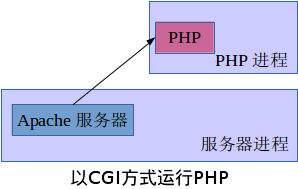
\includegraphics[scale=0.65]{php_cgi.png}
\end{figure}

为了弥补CGI的先天缺陷,以Apache模块方式运行PHP后,动态链接库php5apache2.dll或php4apache2.dll在Aapche服务启动的同时,将会被载入到与Apache服务相同的内存单元中,而且在PHP脚本解析期间不会增加额外的进程。

Apache模块可以在节省资源的同时提高系统运行效率,而且PHP的某些系统特性(例如数据库的持久连接等)只有在以Apache模块形式运行PHP时才会生效。



\begin{figure}[htbp]
\centering
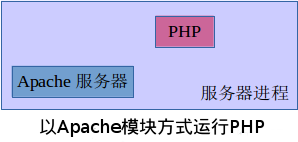
\includegraphics[scale=0.65]{php_apache_module.png}
\end{figure}

\subsection{Request Message}

客户端发起的请求信息(Request Message)包括请求行、(请求)头、空行和其他消息体。

\begin{compactitem}
\item 请求行,例如 GET /images/logo.gif HTTP/1.1 表示从/images 目录下请求 logo.gif文件。
\item (请求)头,例如 Accept-Language: en
\item 空行
\item 其他消息体
\end{compactitem}

请求行和标题必须以 <CR><LF> 作为结尾,空行内必须只有 <CR><LF> 而无其他空格。在 HTTP/1.1 协议中,所有的请求头(除 Host 外)都是可选的。例如,下面是一个HTTP 客户端与服务器之间会话的例子。



\begin{lstlisting}[language=bash]
GET / HTTP/1.1
Host:www.google.com
\end{lstlisting}

在客户端发起的请求的末尾有一个空行(以回车(CR)加换行(LF)的形式表示),其中请求信息的第一行指定方法、资源路径、协议版本,第二行是使用 HTTP/1.1 中必需的 header 来指定主机。

另外,在 HTTP 服务器返回的应答中的文件头之后也使用一个空行来隔开 header 和HTML 代码。




\begin{lstlisting}[language=bash]
HTTP/1.1 200 OK
Content-Length: 3059
Server: GWS/2.0
Date: Sat, 11 Jan 2003 02:44:04 GMT
Content-Type: text/html
Cache-control: private
Set-Cookie: PREF=ID=73d4aef52e57bae9:TM=1042253044:LM=1042253044:S=SMCc_HRPCQiqy
X9j; expires=Sun, 17-Jan-2038 19:14:07 GMT; path=/; domain=.google.com
Connection: keep-alive
<!-- HTML -->
\end{lstlisting}

HTTP/1.1 优化支持持续活跃连接,客户端可以连续多次发送请求、接收应答,而且批量多请求时,同一 TCP 连接在活跃(Keep-Live)间期内可以进行复用来避免重复 TCP初始握手活动,并减少网络负荷和响应周期。

此外,HTTP/1.1 支持应答到达前继续发送请求(通常是两个),称为“流线化”(stream)。

\subsection{Request Method}

HTTP/1.1 协议中共定义了八种方法(也叫“动作”)来以不同方式操作指定的资源。

OPTIONS 方法可使服务器传回该资源所支持的所有 HTTP 请求方法。用’*’ 来代替资源名称向 Web 服务器发送 OPTIONS 请求,则将返回响应的功能和方法,从而可以测试服务器功能是否正常运作。

HEAD 与 GET 方法一样,都是向服务器发出指定资源的请求。不过,服务器将不传回资源的正文部份,只是传回响应客户端请求的文件头,因此使用 HEAD 方法可以在不必传输全部内容的情况下,就可以获取其中“关于该资源的信息”(元信息或称元数据)。

GET 方法向指定的资源发出“显示”请求,因此 GET 方法应该只用在读取数据,而不应当被用于产生“副作用”的操作中。

另外,使用 GET 方法可以在请求 URL 中包含明文变量,一般情况下使用? 和 \&来隔开不同的变量。例如,在请求 URL(http://test.com/index.html?id=003\&title=test)中的变量和值分别为:

\begin{compactitem}
\item id=003
\item title=test
\end{compactitem}

POST 方法向指定资源提交数据并请求服务器进行处理(例如提交表单或者上传文件)。数据被包含在请求本文中,POST 请求可能会创建新的资源或修改现有资源,或二者皆有。

PUT 方法向指定资源位置上传其最新内容。

DELETE 方法请求服务器删除 Request-URI 所标识的资源。

TRACE 方法回显服务器收到的请求,主要用于测试或诊断。

CONNECT 方法由 HTTP/1.1 协议预留给能够将连接改为管道方式的代理服务器。通常用于 SSL 加密服务器的链接(经由非加密的 HTTP 代理服务器)。


请求方法的名称是区分大小写的,这样当某个请求所针对的资源不支持对应的请求方法的时候,服务器应当返回状态码 405(Method Not Allowed),当服务器不认识或者不支持对应的请求方法的时候,应当返回状态码 501(Not Implemented)。

HTTP 服务器至少应该实现 GET 和 HEAD 方法,其他方法都是可选的,而且特定的HTTP 服务器还能够扩展自定义的方法。例如,由 RFC5789 指定的 PATCH 方法用于将局部修改应用到资源。

HTTPS URI 方案和 HTTP 1.1 请求头都可以创建安全超文本协议连接,不过浏览器对后者的几乎没有任何支持,因此 HTTPS URI 方案仍是创建安全超文本协议连接的主要手段。

对于 GET 和 HEAD 方法而言,除了进行获取资源信息外,这些请求不应当再有其他意义。也就是说,这些方法应当被认为是“安全的”。客户端可能会使用其他“非安全”方法(例如 POST,PUT 及 DELETE)以特殊的方式(通常是按钮而不是超链接)来告知客户可能的后果(例如一个按钮控制的资金交易),或请求的操作可能是不安全的(例如某个文件将被上传或删除)。

在不考虑诸如错误或者过期等问题的情况下,若干次请求的副作用与单次请求相同或者根本没有副作用,那么这些请求方法就能够被视作“幂等”的,因此 GET,HEAD,PUT 和 DELETE 等方法都有这样的幂等属性。

假如某个由若干个请求做成的请求序列产生的结果在重复执行这个请求序列或者其中任何一个或多个请求后仍没有发生变化,则这个请求序列便是“幂等”的。但是,可能出现若干个请求做成的请求序列是“非幂等”的,即使这个请求序列中所有执行的请求方法都是幂等的。例如,这个请求序列的结果依赖于某个会在下次执行这个序列的过程中被修改的变量。

\subsection{Request Protocol}

Web 服务器支持的协议包括 HTTP、HTTPS、FTP、Telnet、news 和 gopher 等,并且协议可以指示浏览器使用特定的方法连接到 Web 服务器的特定端口。

使用不同的协议的情况下,浏览器获得的响应数据也是不同的。

通常情况下,Web 服务器根目录下包含特殊的文件(例如 index.html 等),因此 Web服务器在收到客户端请求时会主动以根目录下的文件来输出。

\subsection{UseCanonicalName}

UseCanonicalName字段可以指定Apache如何构造系统的URL、主机名和端口号。

\begin{compactitem}
\item Off说明使用ServerName的值;
\item On说明使用由客户端发送过来的服务器名和端口号。
\end{compactitem}




\subsection{Error Response}

如果网站根目录下找不到首页(index 文件),Web 服务器可能的错误显示方式包括:

\begin{compactitem}
\item 如果在 Options 中设置了 Indexes,那么相应目录下的所有文件都会被列出来,提供类似 FTP 的链接页面。
\item 如果没有指定 Index 则可能显示错误信息通知。
\end{compactitem}

例如,在 httpd.conf 中对错误回应有如下的设置:


\begin{lstlisting}[language=bash]
#
# Customizable error responses come in three flavors:
# 1) plain text 2) local redirects 3) external redirects
#
# Some examples:
#ErrorDocument 500 "The server made a boo boo."
#ErrorDocument 404 /missing.html
#ErrorDocument 404 "/cgi-bin/missing_handler.pl"
#ErrorDocument 402 http://www.example.com/subscription_info.html
#
\end{lstlisting}


在 Web 服务器的所有配置文件中只能有一个 ErrorDocument 设置,如果设置了多个相同的 ErrorDocument 值,则以较晚出现的设置为最终设置。

\begin{compactitem}
\item 100 ~ 199,基本信息
\item 200 ~ 299,客户端请求成功
\item 300 ~ 399,客户端请求需要其他额外的操作(例如重定向等)
\item 400 ~ 499,客户端请求无法完成(例如无法找到文件)
\item 500 ~ 599,Web服务器端错误
\end{compactitem}

\subsection{Access Permission}

Web 服务器的配置文件可以指定限制浏览来源的操作,还可以针对来源 IP 或网段进行限制\footnote{在实际生产环境中设置网段和 IP 的访问权限时,最好使用 iptables 来实现。}。


Apache httpd Server默认情况下的安全设置是拒绝一切访问,例如下面的指令禁止在任一目录下改变认证和访问控制。

\begin{lstlisting}[language=bash]
<Directory />
	Deny from all
	Allow Override None
</Directory>
\end{lstlisting}



默认的访问权限与allow和deny字段的处理顺序有关,而且allow和deny可以指定多个变量,其中:


\begin{compactitem}
\item allow字段用于设置可以访问服务器的客户端;
\item deny字段用于限制访问服务器的客户端。
\end{compactitem}


当deny和allow一起使用时,可以使用Order命令设置deny和allow的结合顺序。

\begin{compactitem}
\item \texttt{Order deny, allow}

以 deny 优先处理,没有写入规则的设置默认为 allow,常用于“拒绝所有,开放特定的条件”。

默认情况下允许所有客户端访问,且deny字段在allow字段之前被匹配。如果既匹配allow字段又匹配allow字段,则allow字段最终生效,也就是说allow覆盖deny。


\begin{lstlisting}[language=bash]
# 仅允许10.0.0.0/8网段的访问
Order deny, allow
Deny from all
Allow from 10.0.0.0/8
\end{lstlisting}

\item \texttt{Order allow, deny}

以 allow 优先处理,没有写入规则的设置默认为 deny,常用于“开放所有,拒绝特定的条件”。


默认情况下拒绝所有客户端访问,且allow字段在deny字段之前被匹配。如果既匹配allow字段又匹配deny字段,则deny字段最终生效,也就是说deny覆盖allow。


\begin{lstlisting}[language=bash]
# 限制www.test.com的访问
Order allow, deny
Allow from all
Deny from www.test.com
\end{lstlisting}

\item 如果 allow 和 deny 的规则中有重复的,则以默认的情况(Order 的规范)为主。
\end{compactitem}

下面的示例中拒绝 10.0.0.5,并对其他所有的主机开放访问,因此需要开放所有并拒绝特定的条件。



\begin{lstlisting}[language=bash]
# vim /etc/httpd/conf/httpd.conf
<Directory "/var/www/html">
	Options FollowSymLinks
	AllowOverride None
	Order allow,deny
	deny from 10.0.0.5
</Directory>
\end{lstlisting}

如果需要对内部受保护的目录(例如/var/www/html/db/进行设置仅有 192.168.1.0/200网段可以访问,可以进行如下的设置:




\begin{lstlisting}[language=bash]
# vim /etc/httpd/conf/httpd.conf
<Directory "/var/www/html/db">
	Options FollowSymLinks
	AllowOverride None
	Order deny, allow
	deny from all
	allow from 192.169.10/200
</Directory>
\end{lstlisting}

除了 Order 设置之外,还可以使用 Limit 来限制客户端能够进行操作的设置。例如,如果设置用户在指定的目录下仅能进行 GET、POST、OPTIONS 等操作,可以使用 Limit和 LimitExcept 如下的设置:


\begin{lstlisting}[language=bash]
# vim /etc/httpd/conf/httpd.conf
<Directory "/var/www/html">
	AllowOverride None
	Options FollowSymLinks
	<Limit GET POST OPTIONS>
		Order allow, deny
		Allow from all
	</Limit>
	<LimitExcept GET POST OPTIONS>
		Order deny, allow
		Deny from all
	</LimitExcept>
</Directory>
\end{lstlisting}

\subsection{User Management}

用户可以为httpd建立专用的用户和组来运行httpd子进程,否则以root用户运行httpd服务容易被攻击者通过漏洞利用或溢出攻击来获得系统的root权限,因此降低运行httpd用户的权限可以使攻击者无法以root身份远程联机或破坏。

在httpd.conf中可以通过User和Group字段分别设置对请求提供服务的httpd子进程运行时的用户和组。

\begin{lstlisting}[language=bash]
#
# If you wish httpd to run as a different user or group, you must run
# httpd as root initially and it will switch.  
#
# User/Group: The name (or #number) of the user/group to run httpd as.
# It is usually good practice to create a dedicated user and group for
# running httpd, as with most system services.
#
User apache
Group apache
# cat /etc/passwd | grep apache
apache:x:48:48:Apache:/usr/share/httpd:/sbin/nologin
\end{lstlisting}




\begin{lstlisting}[language=bash]

\end{lstlisting}




\begin{lstlisting}[language=bash]

\end{lstlisting}




\begin{lstlisting}[language=bash]

\end{lstlisting}




\begin{lstlisting}[language=bash]

\end{lstlisting}




\begin{lstlisting}[language=bash]

\end{lstlisting}




\begin{lstlisting}[language=bash]

\end{lstlisting}




\section{Server Logging}

为系统服务建立日志文件是必不可少的工作,否则网络中针对系统的开放端口的恶意连接尝试等攻击就无法记录,也就无法通过分析日志文件来监控运行状态,也无法分析出错误原因和找出安全隐患,因此在Apache httpd服务中至少要建立访问日志和错误日志文件来记录相关信息。

\begin{compactitem}
\item /var/log/httpd/access\_log 记录客户端正常的请求信息,可以用来分析热门网页等。
\item /var/log/httpd/error\_log 记录服务启动和运行过程中发生的错误、客户端请求错误以及主机设置错误等信息,可以用来检测404错误、文件权限设置错误和密码文件名输入错误等。
\end{compactitem}

\subsection{Error Log}


用户可以通过tail命令来动态检测httpd错误日志来排除故障。



\begin{lstlisting}[language=bash]
# tail -f /var/log/httpd/error_log
[Sun May 03 14:58:07.929011 2015] [mpm_prefork:notice] [pid 1783] AH00163: Apache/2.4.10 (Fedora) OpenSSL/1.0.1k-fips PHP/5.6.8 configured -- resuming normal operations
\end{lstlisting}

\begin{compactitem}
\item 错误发生的时间
\item 错误的级别(或严重性)
\item 错误的进程ID
\item 错误信息
\end{compactitem}


日志文件是纯文本信息而且增长很快,因此需要进行压缩和轮换,Apache 默认提供了/etc/logrotate.d/httpd 来处理日志。其中,开启 compress 可以进行日志压缩。




\begin{lstlisting}[language=bash]
# cat /etc/logrotate.d/httpd
/var/log/httpd/*log {
	missingok
	notifempty
	sharedscripts
	delaycompress
	postrotate
	/bin/systemctl reload httpd.service > /dev/null 2>/dev/null || true
	endscript
	# compress
}
\end{lstlisting}


\subsection{Access Log}


访问日志可以记录服务器处理的所有请求,这样可以检测访问服务器的客户端和被访问的文件。

访问日志的文件名和位置取决于CustomLog字段的设置,默认值如下:


\begin{lstlisting}[language=bash]
# cat /etc/httpd/conf/httpd.conf | grep CustomLog
<IfModule log_config_module>
    #
    # The following directives define some format nicknames for use with
    # a CustomLog directive (see below).
    #
    LogFormat "%h %l %u %t \"%r\" %>s %b \"%{Referer}i\" \"%{User-Agent}i\"" combined
    LogFormat "%h %l %u %t \"%r\" %>s %b" common

    <IfModule logio_module>
      # You need to enable mod_logio.c to use %I and %O
      LogFormat "%h %l %u %t \"%r\" %>s %b \"%{Referer}i\" \"%{User-Agent}i\" %I %O" combinedio
    </IfModule>

    #
    # The location and format of the access logfile (Common Logfile Format).
    # If you do not define any access logfiles within a <VirtualHost>
    # container, they will be logged here.  Contrariwise, if you *do*
    # define per-<VirtualHost> access logfiles, transactions will be
    # logged therein and *not* in this file.
    #
    #CustomLog "logs/access_log" common

    #
    # If you prefer a logfile with access, agent, and referer information
    # (Combined Logfile Format) you can use the following directive.
    #
    CustomLog "logs/access_log" combined
</IfModule>
\end{lstlisting}


combined和common都表示日志采用的格式,其中:

\begin{compactitem}
\item common表示通用日志格式,可以被日志分析识别;
\item combined表示组合类型日志,比通用日志格式增加了“引用页”和“浏览器识别”字段。
\end{compactitem}

访问日志的格式中使用类似printf()函数的格式字符串,使用LogFormat字段可以指定日志的格式和类型。

\begin{compactitem}
\item \%h表示发送请求到服务器的客户端IP地址。
\item \%l表示由客户端identd进程判断的RFC1413身份,不过除非在严格控制的内部网络中,否则\%l通常很不可靠,可以使用\texttt{-\%l}表示信息无效。

实际上,只有在将IndentityCheck指令设置为On时,httpd才会试图得到身份信息。

\item \%u表示HTTP认证系统得到的访问网页的客户标识(userid),例如环境变量REMOTE\_USER会被设置为userid并提供给CGI脚本。

\begin{compactitem}[$\circ$]
\item 如果状态码是401,表示客户未通过认证,那么userid无意义;
\item 如果网页没有设置密码保护,那么可以设置为\texttt{-\%u}。
\end{compactitem}

\item \%t表示服务器完成请求处理时的时间。

\item \texttt{\textbackslash "\%r\textbackslash"}表示客户端发出的包含相关信息的请求行,例如\texttt{GET / HTTP/1.1}。

\item \%>s表示服务器返回给客户端的状态码,可以用来指示请求的结果。

\begin{compactitem}[$\circ$]
\item 100 ~ 199,基本信息
\item 200 ~ 299,客户端请求成功
\item 300 ~ 399,客户端请求需要其他额外的操作(例如重定向等)
\item 400 ~ 499,客户端请求无法完成(例如无法找到文件)
\item 500 ~ 599,Web服务器端错误
\end{compactitem}

\item \%b表示返回给客户端的不包括响应头的字节数,\texttt{-\%b}表示没有信息返回,\texttt{\%B}表示希望记录为“0”的返回信息。

\item \texttt{\textbackslash "\{Referer\}i\textbackslash "}表示提交请求的网页。

\item \texttt{\textbackslash "\%\{User-Agent\}i\textbackslash "}表示客户端提供的浏览器识别信息。

\end{compactitem}

\section{Directory}





通常情况下,在访问某个网站时真正访问的仅仅是Web服务器中某个目录下的某个网页文件,不同的目录和文件组成了最终的网站。

在httpd.conf中基于目录块可以使用<Directory>对目录进行配置,而且<Directory>段中的命令的作用域是指定的目录及其所有子目录,不过使用.htaccess可以实现相同的效果。


\begin{lstlisting}[language=bash]
<Directory 目录>
控制语句
</Directory>
\end{lstlisting}

在设置网站整体的权限之外,可以使用由成对出现的<Directory></Directory>表示的Directory容器修改目录的权限。例如,下面的设置可以拒绝192.168.1.100的客户端访问某个目录内的文件。


\begin{lstlisting}[language=bash]
<Directory /doc>
	Order allow, deny
	Allow from all
	Deny from 192.168.1.100
</Directory>
\end{lstlisting}




\subsection{Root Directory}

下面是根目录默认设置:

\begin{lstlisting}[language=bash]
<Directory />
    AllowOverride none
    Require all denied
</Directory>
\end{lstlisting}

\begin{table}[htbp]
\centering
\caption{Options常用设置}
\begin{tabular}{|l|l|}
\hline
Options & 备注\\
\hline
FollowSymLinks & 允许在目录中使用符号链接\\
\hline
Indexes & 允许目录浏览,可以列出目录结构和子目录和文件\\
\hline
MultiViews & 允许内容协商的多重视图,例如提供多语言支持等\\
\hline
ExecCGI&允许执行CGI脚本\\
\hline
Includes & 允许服务器端包含(SSI)功能,和IIS/PWS的shtml功能相同\\
\hline
IncludesNoExec&允许服务器端包含(SSI)功能,但是不能执行CGI脚本\\
\hline
ALL&包含除MultiViews之外的所有特性。如果没有Options字段,默认为ALL\\
\hline
\end{tabular}
\end{table}

AllowOverride用于指定.htaccesss文件文件中的指令类型,从而限制.htaccess对相应类型命令的控制权。

\begin{compactitem}
\item None表示禁止使用.htaccess;
\item Options允许使用指定目录控制功能的命令;
\item Indexes允许使用目录索引类命令;
\item AuthConfig允许使用权限识别命令;
\item FileInfo允许使用文档控制类命令;
\item Limit允许使用主机访问控制类命令(Allow、Deny和Order)。
\end{compactitem}

默认情况下,Apache服务器允许使用.htaccess(即访问控制文件)对任意目录进行单独设置来覆盖主配置文件中的设置,而且修改.htaccess后可以即时生效,无需重启Apache服务器。

在启用CGI方式处理网络请求时,应该只允许特定的目录(例如cgi-bin)执行CGI功能,以防受到恶意攻击。

IncludesNoExec禁用“\#exec”和“\#exec CGI”,可以从ScriptAlias目录使用“\#include”虚拟CGI脚本。





\subsection{Document Directory}

下面是文档目录的默认设置:

\begin{lstlisting}[language=bash]
#
# Relax access to content within /var/www.
#
<Directory "/var/www">
    AllowOverride None
    # Allow open access:
    Require all granted
</Directory>

# Further relax access to the default document root:
<Directory "/var/www/html">
    #
    # Possible values for the Options directive are "None", "All",
    # or any combination of:
    #   Indexes Includes FollowSymLinks SymLinksifOwnerMatch ExecCGI MultiViews
    #
    # Note that "MultiViews" must be named *explicitly* --- "Options All"
    # doesn't give it to you.
    #
    # The Options directive is both complicated and important.  Please see
    # http://httpd.apache.org/docs/2.4/mod/core.html#options
    # for more information.
    #
    Options Indexes FollowSymLinks

    #
    # AllowOverride controls what directives may be placed in .htaccess files.
    # It can be "All", "None", or any combination of the keywords:
    #   Options FileInfo AuthConfig Limit
    #
    AllowOverride None

    #
    # Controls who can get stuff from this server.
    #
    Require all granted
</Directory>
\end{lstlisting}

\subsection{Directory Alias}

一般情况下,httpd 服务器默认的文档根目录为/var/www/html,如果需要发布到其他目录需要使用虚拟目录(alias)功能。


虚拟目录就是给一个实际目录起一个别名,这样就可以把不在文档目录中的目录纳入httpd服务管理。



\begin{lstlisting}[language=bash]
# phpMyAdmin - Web based MySQL browser written in php
# 
# Allows only localhost by default
#
# But allowing phpMyAdmin to anyone other than localhost should be considered
# dangerous unless properly secured by SSL

Alias /phpMyAdmin /usr/share/phpMyAdmin
Alias /phpmyadmin /usr/share/phpMyAdmin
\end{lstlisting}

\begin{compactitem}
\item 虚拟目录的名称和路径都不受实际目录名称和路径的限制,客户端不区分虚拟目录和实际目录。

\item 虚拟目录可以用于视频点播网站等需要大容量存储空间的硬盘扩容。

\item 虚拟目录不受目录移动和重命名等的限制,不会影响用户的访问。

\item 虚拟目录可以设置和实际目录相同的权限,并且攻击者无法猜测虚拟目录的实际路径。

\end{compactitem}

\begin{lstlisting}[language=bash]

\end{lstlisting}



\begin{lstlisting}[language=bash]

\end{lstlisting}



\begin{lstlisting}[language=bash]

\end{lstlisting}



\begin{lstlisting}[language=bash]

\end{lstlisting}



\begin{lstlisting}[language=bash]

\end{lstlisting}




\subsection{File Permission}

如果仅对某个文件设置权限,可以使用由成对出现的<Files></Files>表示的Files容器修改权限。


\begin{lstlisting}[language=bash]
<Files ~ "/var/www/html/robot.txt">
	Order allow, deny
	Allow from all
</Files>
\end{lstlisting}



\begin{lstlisting}[language=bash]

\end{lstlisting}

\section{Virtualhost}



虚拟主机(Virtual Host)让多个主机名称(host name)运行在在单一服务器(或是服务器组)上,从而实现多个域名和主机名绑定,而且可以单独支持每个单一的主机名称。

通过将服务器的某项或者全部服务内容逻辑划分为多个服务单位,对外可以表现为多个服务器,从而充分利用服务器硬件资源。如果划分是系统级别的,则称为虚拟服务器。例如,如果使用 dig 等检查 IP,可能发现不同的网址可能指向同一个 IP。

单一主机(或服务器组)支撑的所有的虚拟主机中,彼此之间可以共用相同的配置设置。另外,相同主机内的虚拟主机可以共用彼此的程序集(Process Pool),从而可以缩短对客户端的响应时间。

虚 拟 主 机 的 实 现 方 式 主 要 有 三 种: 网 址 名 称 对 应 (Name-based)、IP 地 址 对 应(IP-based)以及 Port 端口号对应(Port-based)。

\begin{compactitem}
\item 网址名称对应(Name-based)

网址名称对应(Name-based)通过辨识客户端所提供的网址来决定其所对应的服务,可以有效的减少 IP 地址的占用,缺点是必须仰赖 DNS 名称对应服务的支持。

若 DNS 服务中断,则对应此名称的服务也会无法取用。

\item IP 地址对应(IP-based)

IP 地址对应(IP-based)是指在同一部服务器上,借由同一份配置设置、不同的 IP来管理多个服务。

\item Port 端口号对应(Port-based)

近似于 IP 地址对应,不过是在同一个 IP 之下利用不同的 Port 端口号来区别不同的服务,藉以快速创建多个虚拟主机。例如:

\begin{lstlisting}[language=bash]
192.168.0.1:80
192.168.0.1:8080
192.168.0.1:8888
\end{lstlisting}

\end{compactitem}



如果每个网站拥有不同的 IP 地址,则虚拟主机可以是” 基于 IP” 的;如果只有一个IP 地址,也可以是” 基于主机名” 的,其实对最终用户是透明的。例如,Apache 是率先支持基于 IP 的虚拟主机的服务器之一,1.1 及其更新版本同时支持基于 IP 和基于主机名的虚拟主机。

如果要调试虚拟主机配置,可以使用 httpd 的-S 命令行开关来输出虚拟主机的配置。






\begin{lstlisting}[language=bash]
// a synonym for -t -D DUMP_VHOSTS -D DUMP_RUN_CFG
# /usr/sbin/httpd -S
VirtualHost configuration:
ServerRoot: "/etc/httpd"
Main DocumentRoot: "/var/www/html"
Main ErrorLog: "/etc/httpd/logs/error_log"
Mutex authdigest-client: using_defaults
Mutex lua-ivm-shm: using_defaults
Mutex proxy: using_defaults
Mutex authn-socache: using_defaults
Mutex default: dir="/run/httpd/" mechanism=default
Mutex mpm-accept: using_defaults
Mutex authdigest-opaque: using_defaults
Mutex proxy-balancer-shm: using_defaults
Mutex rewrite-map: using_defaults
PidFile: "/run/httpd/httpd.pid"
Define: DUMP_VHOSTS
Define: DUMP_RUN_CFG
User: name="apache" id=48
Group: name="apache" id=48
\end{lstlisting}


一般情况下,虚拟主机的配置文件 vhosts.conf 保存为/etc/httpd/conf.d/vhosts.conf,而且虚拟主机的设置中至少要有 ServerName 和 DocumentRoot。

如果没有针对 SELinux 设置 httpd 可以读取的文件系统,则虚拟主机无法提供浏览功能。


\subsection{IP}


下面的示例说明使用httpd实现基于IP的虚拟主机,这样需要为Web服务器的网卡绑定多个IP地址。


\begin{lstlisting}[language=bash]
# ifconfig eth0:0 192.168.1.11 netmask 255.255.255.0
# ifconfig eth0:1 192.168.1.12 netmask 255.255.255.0

# cat > /etc/httpd/conf/httpd.conf
...

<VirtualHost 192.168.1.10:80>
	DocumentRoot /var/www/html/www.example.com
	ServerName www.example.com
</VirtualHost>

<VirtualHost 192.168.1.11:80>
	DocumentRoot /var/www/html/bbs.example.com
	ServerName bbs.example.com
</VirtualHost>

<VirtualHost 192.168.1.12:80>
	DocumentRoot /var/www/html/test.example.com
	ServerName test.example.com
</VirtualHost>

# mkdir -p /var/www/html/www.example.com
# mkdir -p /var/www/html/bbs.example.com
# mkdir -p /var/www/html/test.example.com

# echo "Welcome to www.example.com" > /var/www/html/www.example.com/index.html
# echo "Welcome to bbs.example.com" > /var/www/html/bbs.example.com/index.html
# echo "Welcome to test.example.com" > /var/www/html/test.example.com/index.html

# chmod -R 755 /var/www/html/bbs.example.com
# chmod -R 755 /var/www/html/test.example.com
\end{lstlisting}




\begin{lstlisting}[language=bash]

\end{lstlisting}





\begin{lstlisting}[language=bash]

\end{lstlisting}





\begin{lstlisting}[language=bash]

\end{lstlisting}





\begin{lstlisting}[language=bash]

\end{lstlisting}



\subsection{Domain}


随着基于IP地址的虚拟主机的增加,采用IP地址的方式会导致IP地址的极大浪费,因此通常情况下都是基于域名来实现虚拟主机。


在主配置文件中添加NameVirtualHost字段,这样就可以为多个虚拟主机统一配置端口,从而就可以开启基于域名的虚拟主机功能。例如,在下面的示例中可以为虚拟主机建立相应的站点目录,设置网页文件,并且所有的域名(这里是www.example.com、bbs.example.com、test.example.com)都可以指向服务器的IP地址,从而完成虚拟主机的配置。


\begin{lstlisting}[language=bash]
# cat > /etc/httpd/conf/httpd.conf
...
NameVirtualHost *:80
<VirtualHost *:80>
	ServerName www.example.com
	DocumentRoot /var/www/html/www.example.com/
</VirtualHost>

<VirtualHost *:80>
	ServerName bbs.example.com
	DocumentRoot /var/www/html/bbs.example.com/
</VirtualHost>

<VirtualHost *:80>
	ServerName test.example.com
	DocumentRoot /var/www/html/test.example.com/
</VirtualHost>
\end{lstlisting}




\begin{lstlisting}[language=bash]

\end{lstlisting}




\begin{lstlisting}[language=bash]

\end{lstlisting}


\section{Module}

\subsection{Extension}

httpd 的主要配置文件位于/etc/httpd/conf/httpd.conf,其他的配置文件则位于/etc/httpd/conf.d/*.conf。


\begin{lstlisting}[language=bash]
$ ll /etc/httpd/conf.d/
-rw-r--r--. 1 root root 2893 Jul 23 18:29 autoindex.conf
-rw-r--r--. 1 root root 295 Jul 23 18:24 manual.conf
-rw-r--r--. 1 root root 747 Nov 21 20:09 php.conf
-rw-r--r--. 1 root root 366 Jul 23 18:31 README
-rw-r--r--. 1 root root 298 Sep 12 18:59 squid.conf
-rw-r--r--. 1 root root 1252 Jul 23 18:24 userdir.conf
-rw-r--r--. 1 root root 516 Jul 23 18:24 welcome.conf
\end{lstlisting}


httpd 本身只支持静态网页文件,如果需要处理动态网页则需要配合相应的模块,这些模块一般位于/usr/lib/httpd/modules(或/usr/lib64/httpd/modules)。


\begin{lstlisting}[language=bash]
$ ll /usr/lib64/httpd/modules
-rwxr-xr-x. 1 root root 4347080 Nov 21 20:10 libphp5.so
-rwxr-xr-x. 1 root root 4561080 Nov 21 20:10 libphp5-zts.so
-rwxr-xr-x. 1 root root 11208 Jul 23 18:31 mod_access_compat.so
-rwxr-xr-x. 1 root root 11168 Jul 23 18:31 mod_actions.so
-rwxr-xr-x. 1 root root 15368 Jul 23 18:31 mod_alias.so
-rwxr-xr-x. 1 root root 11144 Jul 23 18:31 mod_allowmethods.so
-rwxr-xr-x. 1 root root 11088 Jul 23 18:31 mod_asis.so
-rwxr-xr-x. 1 root root 15360 Jul 23 18:31 mod_auth_basic.so
-rwxr-xr-x. 1 root root 36056 Jul 23 18:31 mod_auth_digest.so
-rwxr-xr-x. 1 root root 11152 Jul 23 18:31 mod_authn_anon.so
-rwxr-xr-x. 1 root root 15368 Jul 23 18:31 mod_authn_core.so
-rwxr-xr-x. 1 root root 15272 Jul 23 18:31 mod_authn_dbd.so
-rwxr-xr-x. 1 root root 11192 Jul 23 18:31 mod_authn_dbm.so
-rwxr-xr-x. 1 root root 11168 Jul 23 18:31 mod_authn_file.so
-rwxr-xr-x. 1 root root 19544 Jul 23 18:31 mod_authn_socache.so
-rwxr-xr-x. 1 root root 23728 Jul 23 18:31 mod_authz_core.so
-rwxr-xr-x. 1 root root 15320 Jul 23 18:31 mod_authz_dbd.so
-rwxr-xr-x. 1 root root 15304 Jul 23 18:31 mod_authz_dbm.so
-rwxr-xr-x. 1 root root 15296 Jul 23 18:31 mod_authz_groupfile.so
-rwxr-xr-x. 1 root root 11200 Jul 23 18:31 mod_authz_host.so
-rwxr-xr-x. 1 root root 11136 Jul 23 18:31 mod_authz_owner.so
-rwxr-xr-x. 1 root root 11160 Jul 23 18:31 mod_authz_user.so
-rwxr-xr-x. 1 root root 40072 Jul 23 18:31 mod_autoindex.so
-rwxr-xr-x. 1 root root 11152 Jul 23 18:31 mod_buffer.so
-rwxr-xr-x. 1 root root 36096 Jul 23 18:31 mod_cache_disk.so
-rwxr-xr-x. 1 root root 77320 Jul 23 18:31 mod_cache.so
-rwxr-xr-x. 1 root root 36064 Jul 23 18:31 mod_cache_socache.so
-rwxr-xr-x. 1 root root 36088 Jul 23 18:31 mod_cgid.so
-rwxr-xr-x. 1 root root 27712 Jul 23 18:31 mod_cgi.so
-rwxr-xr-x. 1 root root 23600 Jul 23 18:31 mod_charset_lite.so
-rwxr-xr-x. 1 root root 11096 Jul 23 18:31 mod_data.so
-rwxr-xr-x. 1 root root 56984 Jul 23 18:31 mod_dav_fs.so
-rwxr-xr-x. 1 root root 19632 Jul 23 18:31 mod_dav_lock.so
-rwxr-xr-x. 1 root root 101992 Jul 23 18:31 mod_dav.so
-rwxr-xr-x. 1 root root 23568 Jul 23 18:31 mod_dbd.so
-rwxr-xr-x. 1 root root 35944 Jul 23 18:31 mod_deflate.so
-rwxr-xr-x. 1 root root 11176 Jul 23 18:31 mod_dialup.so
-rwxr-xr-x. 1 root root 15288 Jul 23 18:31 mod_dir.so
-rwxr-xr-x. 1 root root 11192 Jul 23 18:31 mod_dumpio.so
-rwxr-xr-x. 1 root root 11160 Jul 23 18:31 mod_echo.so
-rwxr-xr-x. 1 root root 11176 Jul 23 18:31 mod_env.so
-rwxr-xr-x. 1 root root 15320 Jul 23 18:31 mod_expires.so
-rwxr-xr-x. 1 root root 23552 Jul 23 18:31 mod_ext_filter.so
-rwxr-xr-x. 1 root root 15408 Jul 23 18:31 mod_file_cache.so
-rwxr-xr-x. 1 root root 19424 Jul 23 18:31 mod_filter.so
-rwxr-xr-x. 1 root root 23752 Jul 23 18:31 mod_headers.so
-rwxr-xr-x. 1 root root 11192 Jul 23 18:31 mod_heartbeat.so
-rwxr-xr-x. 1 root root 23592 Jul 23 18:31 mod_heartmonitor.so
-rwxr-xr-x. 1 root root 52520 Jul 23 18:31 mod_include.so
-rwxr-xr-x. 1 root root 28120 Jul 23 18:31 mod_info.so
-rwxr-xr-x. 1 root root 11136 Jul 23 18:31 mod_lbmethod_bybusyness.so
-rwxr-xr-x. 1 root root 11136 Jul 23 18:31 mod_lbmethod_byrequests.so
-rwxr-xr-x. 1 root root 11128 Jul 23 18:31 mod_lbmethod_bytraffic.so
-rwxr-xr-x. 1 root root 15320 Jul 23 18:31 mod_lbmethod_heartbeat.so
-rwxr-xr-x. 1 root root 28192 Jul 23 18:31 mod_log_config.so
-rwxr-xr-x. 1 root root 15392 Jul 23 18:31 mod_log_debug.so
-rwxr-xr-x. 1 root root 11216 Jul 23 18:31 mod_log_forensic.so
-rwxr-xr-x. 1 root root 11232 Jul 23 18:31 mod_logio.so
-rwxr-xr-x. 1 root root 133424 Jul 23 18:31 mod_lua.so
-rwxr-xr-x. 1 root root 19440 Jul 23 18:31 mod_macro.so
-rwxr-xr-x. 1 root root 27736 Jul 23 18:31 mod_mime_magic.so
-rwxr-xr-x. 1 root root 23616 Jul 23 18:31 mod_mime.so
-rwxr-xr-x. 1 root root 60960 Jul 23 18:31 mod_mpm_event.so
-rwxr-xr-x. 1 root root 31880 Jul 23 18:31 mod_mpm_prefork.so
-rwxr-xr-x. 1 root root 48432 Jul 23 18:31 mod_mpm_worker.so
-rwxr-xr-x. 1 root root 36000 Jul 23 18:31 mod_negotiation.so
-rwxr-xr-x. 1 root root 52136 Jul 23 18:31 mod_proxy_ajp.so
-rwxr-xr-x. 1 root root 48176 Jul 23 18:31 mod_proxy_balancer.so
-rwxr-xr-x. 1 root root 19400 Jul 23 18:31 mod_proxy_connect.so
-rwxr-xr-x. 1 root root 15280 Jul 23 18:31 mod_proxy_express.so
-rwxr-xr-x. 1 root root 19376 Jul 23 18:31 mod_proxy_fcgi.so
-rwxr-xr-x. 1 root root 11152 Jul 23 18:31 mod_proxy_fdpass.so
-rwxr-xr-x. 1 root root 44184 Jul 23 18:31 mod_proxy_ftp.so
-rwxr-xr-x. 1 root root 39944 Jul 23 18:31 mod_proxy_http.so
-rwxr-xr-x. 1 root root 19464 Jul 23 18:31 mod_proxy_scgi.so
-rwxr-xr-x. 1 root root 118608 Jul 23 18:31 mod_proxy.so
-rwxr-xr-x. 1 root root 19352 Jul 23 18:31 mod_proxy_wstunnel.so
-rwxr-xr-x. 1 root root 11128 Jul 23 18:31 mod_ratelimit.so
-rwxr-xr-x. 1 root root 11160 Jul 23 18:31 mod_reflector.so
-rwxr-xr-x. 1 root root 15304 Jul 23 18:31 mod_remoteip.so
-rwxr-xr-x. 1 root root 15320 Jul 23 18:31 mod_reqtimeout.so
-rwxr-xr-x. 1 root root 15344 Jul 23 18:31 mod_request.so
-rwxr-xr-x. 1 root root 69032 Jul 23 18:31 mod_rewrite.so
-rwxr-xr-x. 1 root root 40312 Jul 23 18:31 mod_sed.so
-rwxr-xr-x. 1 root root 15328 Jul 23 18:31 mod_setenvif.so
-rwxr-xr-x. 1 root root 11240 Jul 23 18:31 mod_slotmem_plain.so
-rwxr-xr-x. 1 root root 19488 Jul 23 18:31 mod_slotmem_shm.so
-rwxr-xr-x. 1 root root 15328 Jul 23 18:31 mod_socache_dbm.so
-rwxr-xr-x. 1 root root 11192 Jul 23 18:31 mod_socache_memcache.so
-rwxr-xr-x. 1 root root 23568 Jul 23 18:31 mod_socache_shmcb.so
-rwxr-xr-x. 1 root root 15272 Jul 23 18:31 mod_speling.so
-rwxr-xr-x. 1 root root 23448 Jul 23 18:31 mod_status.so
-rwxr-xr-x. 1 root root 15272 Jul 23 18:31 mod_substitute.so
-rwxr-xr-x. 1 root root 11168 Jul 23 18:31 mod_suexec.so
-rwxr-xr-x. 1 root root 11112 Jul 23 18:31 mod_systemd.so
-rwxr-xr-x. 1 root root 11144 Jul 23 18:31 mod_unique_id.so
-rwxr-xr-x. 1 root root 15312 Jul 23 18:31 mod_unixd.so
-rwxr-xr-x. 1 root root 11168 Jul 23 18:31 mod_userdir.so
-rwxr-xr-x. 1 root root 15320 Jul 23 18:31 mod_usertrack.so
-rwxr-xr-x. 1 root root 11104 Jul 23 18:31 mod_version.so
-rwxr-xr-x. 1 root root 15280 Jul 23 18:31 mod_vhost_alias.so
-rwxr-xr-x. 1 root root 19480 Jul 23 18:31 mod_watchdog.so
\end{lstlisting}

用户可通过简单的 API 扩充,将 Perl/Python/PHP 等解释器编译到 HTTP 服务器中。例如,httpd 使用的 PHP 模块就是/usr/lib64/httpd/modules/libphp5.so,相应的 PHP 设置文件则位于/etc/httpd/conf.d/php.conf,并且在其中设置了由 PHP 产生的 session和 soap 的存储目录等信息。


\begin{lstlisting}[language=bash]
$ vim /etc/httpd/conf.d/php.conf
#
# Cause the PHP interpreter to handle files with a .php extension.
#
<FilesMatch \.php$>
	SetHandler application/x-httpd-php
</FilesMatch>
#
# Allow php to handle Multiviews
#
AddType text/html .php
#
# Add index.php to the list of files that will be served as directory indexes.
#
DirectoryIndex index.php
#
# Uncomment the following lines to allow PHP to pretty-print .phps files as PHP source code:
#
#<FilesMatch \.phps$>
#
SetHandler application/x-httpd-php-source
#</FilesMatch>
#
# Apache specific PHP configuration options those can be override in each configured vhost
#
php_value session.save_handler "files"
php_value session.save_path "/var/lib/php/session"
php_value soap.wsdl_cache_dir "/var/lib/php/wsdlcache"
\end{lstlisting}

不过,PHP 本身的主要配置文件为/etc/php.ini,其中包含了 PHP 的全部设置选项。

对于 PHP 的额外扩展配置则保存在/etc/php.d 和/etc/php-zts.d 中。


\begin{lstlisting}[language=bash]
$ ll /etc/php.d
-rw-r--r--. 1 root root 47 Nov 21 20:09 bz2.ini
-rw-r--r--. 1 root root 57 Nov 21 20:09 calendar.ini
-rw-r--r--. 1 root root 51 Nov 21 20:09 ctype.ini
-rw-r--r--. 1 root root 49 Nov 21 20:09 curl.ini
-rw-r--r--. 1 root root 47 Nov 21 20:09 dom.ini
-rw-r--r--. 1 root root 49 Nov 21 20:09 exif.ini
-rw-r--r--. 1 root root 57 Nov 21 20:09 fileinfo.ini
-rw-r--r--. 1 root root 47 Nov 21 20:09 ftp.ini
-rw-r--r--. 1 root root 55 Nov 21 20:09 gettext.ini
-rw-r--r--. 1 root root 51 Nov 21 20:09 iconv.ini
-rw-r--r--. 1 root root 51 Aug 1 14:50 json.ini
-rw-r--r--. 1 root root 55 Nov 21 20:09 mysqlnd.ini
-rw-r--r--. 1 root root 69 Nov 21 20:09 mysqlnd_mysqli.ini
-rw-r--r--. 1 root root 67 Nov 21 20:09 mysqlnd_mysql.ini
-rw-r--r--. 1 root root 47 Nov 21 20:09 pdo.ini
-rw-r--r--. 1 root root 63 Nov 21 20:09 pdo_mysqlnd.ini
-rw-r--r--. 1 root root 61 Nov 21 20:09 pdo_sqlite.ini
-rw-r--r--. 1 root root 49 Nov 21 20:09 phar.ini
-rw-r--r--. 1 root root 51 Nov 21 20:09 posix.ini
-rw-r--r--. 1 root root 51 Nov 21 20:09 shmop.ini
-rw-r--r--. 1 root root 59 Nov 21 20:09 simplexml.ini
-rw-r--r--. 1 root root 55 Nov 21 20:09 sockets.ini
-rw-r--r--. 1 root root 55 Nov 21 20:09 sqlite3.ini
-rw-r--r--. 1 root root 55 Nov 21 20:09 sysvmsg.ini
-rw-r--r--. 1 root root 55 Nov 21 20:09 sysvsem.ini
-rw-r--r--. 1 root root 55 Nov 21 20:09 sysvshm.ini
-rw-r--r--. 1 root root 59 Nov 21 20:09 tokenizer.ini
-rw-r--r--. 1 root root 101 Nov 17 20:47 xdebug.ini
-rw-r--r--. 1 root root 47 Nov 21 20:09 xml.ini
-rw-r--r--. 1 root root 59 Nov 21 20:09 xmlreader.ini
-rw-r--r--. 1 root root 49 Nov 21 20:09 xml_wddx.ini
-rw-r--r--. 1 root root 59 Nov 21 20:09 xmlwriter.ini
-rw-r--r--. 1 root root 47 Nov 21 20:09 xsl.ini
\end{lstlisting}

一般情况下,httpd 服务器默认的文档根目录为/var/www/html,其中的设置包括:

\begin{compactitem}
\item 错误信息位于/var/www/error
\item CGI 位于/var/www/cgi-bin
\item 图标位于/var/www/icons
\item 日志文件位于/var/log/httpd
\end{compactitem}

httpd 的可执行文件为/usr/sbin/httpd,而且其主要的环境检测和执行文件是/usr/sbin/apachectl,用于在启动 httpd 服务器时检测系统设置。

httpd 本身提供了基本的密码保护方式,这样就可以在用户登录某些网页时进行帐号/密码验证,其中密码使用/usr/bin/htpasswd 来产生。

如果使用 MySQL 数据库,则其配置文件位于/etc/my.conf,默认情况下数据库位于/var/lib/mysql。其中,与 PHP 配合使用的 MySQL 接口文件位于/usr/lib64/mysql。

为了产生由 MySQL 数据库驱动的 PHP 应用程序,需要在相应的配置中中对 PHP 支持的 MySQL 接口等进行设置。

\begin{compactitem}
\item /etc/php.d/mysqlnd.ini
\item /etc/php.d/mysqlnd\_mysqli.ini
\item /etc/php.d/mysqlnd\_mysql.ini
\item /etc/php.d/pdo\_mysqlnd.ini
\end{compactitem}

PHP 是动态语言,其程序中的值需要在运行时才能确定,因此如果需要安装 PHP 加速器等组件时需要/usr/bin/phpize 来辅助 PHP 扩展的编译。

一般情况下,编译安装 PHP 扩展时需要的头文件等都位于/usr/include/php 中。


\subsection{mod\_pagespeed}


PageSpeed (mod\_pagespeed) 是 Google开放的网页加速模块,支持Apache和Nginx服务器。 

64位系统:

\begin{lstlisting}[language=bash]
# wget https://dl-ssl.google.com/dl/linux/direct/mod-pagespeed-stable_current_x86_64.rpm
# rpm -ivh mod-pagespeed-stable_current_x86_64.rpm
\end{lstlisting}

32位系统:


\begin{lstlisting}[language=bash]
# wget https://dl-ssl.google.com/dl/linux/direct/mod-pagespeed-stable_current_i386.rpm
# rpm -ivh mod-pagespeed-stable_current_i386.rpm
\end{lstlisting}


如果把Pagespeed模块的仓库文件存到/etc/yum.repos.d/,这样就可以使用YUM来安装mode\_pagespeed。

\begin{lstlisting}[language=bash]
$ sudo yum install mod-pagespeed
\end{lstlisting}

用户可以通过/etc/httpd/conf.d/目录下的pagespeed.conf和pagespeed\_libraries.conf文件来设置mod\_pagespeed,并且通过重启Apache服务器来使配置生效。


\subsection{mod\_security}

mod\_security是Apache的安全模块,可以预防多种针对网页的攻击,例如远程代码执行、SQL注入和路径扫描等。




\begin{lstlisting}[language=bash]

\end{lstlisting}

用户可以直接下载并安装mod\_security模块:

CentOS/RHEL:


\begin{lstlisting}[language=bash]
$ sudo yum install mod_security
$ sudo systemctl restart httpd
\end{lstlisting}



Debian/Ubuntu

\begin{lstlisting}[language=bash]
$ sudo apt-get install libapache-mod-security
$ sudo a2enmod mod-security
$ sudo /etc/init.d/apache2 force-reload
\end{lstlisting}


也可以下载mod\_security的源代码并进行编译安装。


\begin{lstlisting}[language=bash]
$ sudo yum install gcc make httpd-devel libxml2 pcre-devel libxml2-devel curl-devel git
$ wget https://www.modsecurity.org/tarball/2.9.0/modsecurity-2.9.0.tar.gz
$ tar xzf modsecurity-apache_2.9.0.tar.gz
$ cd modsecurity-apache_2.9.0
$ ./configure
$ make && sudo make install
$ sudo cp modsecurity.conf-recommended /etc/httpd/conf.d/modsecurity.conf
$ sudo cp unicode.mapping /etc/httpd/conf.d/
\end{lstlisting}


在/etc/httpd/httpd.conf中加入mod\_security模块的配置信息来通过重启Apache载入mod\_security。


\begin{lstlisting}[language=bash]
LoadModule security2_module modules/mod_security2.so
<IfModule security2_module>
    Include conf.d/modsecurity.conf
</IfModule>
 
Include modsecurity-crs/modsecurity_crs_10_config.conf
Include modsecurity-crs/base_rules/*.conf
\end{lstlisting}






\begin{lstlisting}[language=bash]

\end{lstlisting}




\begin{lstlisting}[language=bash]

\end{lstlisting}





\begin{lstlisting}[language=bash]

\end{lstlisting}




\begin{lstlisting}[language=bash]

\end{lstlisting}





\section{Security}



使用 HTTP 协议来传输数据时都是以明文传送的,HTTPS 协议使用 SSL 加密机制来传输数据。



如果客户端和服务器同时支持 SSL(Secure Socket Layer)协议,那么服务器将产生公钥并向 CA(Certificate Authorities)注册,客户端浏览器可以主动向 CA 确认服务器端的公钥是否是合法的,如果合法则建立与服务器的连接,否则将发出警告信息来告知用户。

\subsection{Encryption}

为了保证机密信息被安全传输,并且有效识别双方的身份,数据加密和数字签名技术被引入到Web客户端和服务器中来对数据进行加密和签名。

\begin{compactitem}
\item 数据加密技术可以防止合法接收者之外的人获取信息系统中的机密信息。

\item 数字签名技术可以使用数字证书来对信息进行签名以实现信息的不可否认性。
\end{compactitem}

用户使用数学方法对原始信息进行加密来实现数据的再组织,使得重组后在网络上公开传输的内容变成对于非法接收者来说无效的信息,只有掌握正确的密钥的合法的接收者才能通过解密来得到原始数据。

\begin{compactitem}
\item 对称加密技术(例如DES)的发送方使用的加密密钥和接收方使用的解密密钥是相同的。

\item 非对称加密技术(例如RSA)要求密钥成对出现并彼此关联,其中用于加密的公钥可以对外界公开,但是用于解密的私钥必须由接收者自己保管。
\end{compactitem}

\subsection{Signature}

在信息传输过程中,单纯采用加密来保证数据的保密性还是存在缺陷的,无法证明信息的发送方身份。

为了使信息(例如合同和钱款往来)无法否认,可以使用数字签名(Digital Signature)技术来保证信息是由签名者自己签名发送的,而且接收方可以验证信息自签发后是否进行过任何修改。

数字签名的过程就是发送者根据待发送的信息和用自身私钥加密的数字摘要组合成数字签名,私钥仅为发送者本人所有,因此可以产生别人无法生成的文件,也就实现了数字签名。



\begin{compactitem}
\item 签名者不能否认或难以否认数字签名;
\item 接收方可以通过检查真实签发的数字证书文件来验证数据完整性。
\end{compactitem}

数字证书(Digital Certificate)是一个经证书授权中心数字签名的包含公开密钥拥有着信息以及公开密钥的文件,最简单的证书包含一个公开密钥、名称以及证书授权中心的数字签名,因此数字证书是标志网络用户身份信息的一系列数据,可以用来在网络通信中识别通信各方的身份。例如,现实中的每一个公司都要拥有工商执照来表明各自的身份或某种资格。

以数字证书为核心的加密技术可以对网络上传输的信息进行加密和解密、数字签名和签名验证,确保网上传递信息的机密性、完整性,交易实体身份的真实性,以及签名信息的不可否认性,从而保障网络应用的安全性。

数字证书签发机构(Certification Authority)管理数字证书的申请者发放、管理和取消,因此和现实中的工商业管理机构——工商行政管理局的职能类似,它们都可以检查证书持有者身份的合法性,并签发证书(用数学方法在证书上签名)来防止证书被伪造或篡改。

SSL(Secure Sockets Layer)是一种国际标准的加密和身份认证通信协议,可以用于Web浏览器和服务器之间的身份认证和加密数据传输,这样SSL通过数字证书和加密技术来实现在Web浏览器和服务器之间的通信无法被窃听,从而为通信双方建立起安全的、可信任的信息通道。

SSL最初由Netscape开发并内置于浏览器中来对数据进行压缩和加密操作,并返回通过网络传送回的数据,HTTPS(HTTP Secure)开始时就是使用SSL作为HTTP应用层的子层。

TLS(Transport Layer Security)及其前身 SSL(Secure Sockets Layer)是一种为互联网通信提供安全及数据完整性保障安全协议。

openssl命令可以为CA创建一个RSA私有密钥,也可以查看密钥的内容。



\begin{lstlisting}[language=bash]
# openssl genrsa -des3 -out ca.key 1024
Generating RSA private key, 1024 bit long modulus
.............++++++
..............................++++++
e is 65537 (0x10001)
Enter pass phrase for ca.key:
Verifying - Enter pass phrase for ca.key:
# chmod 400 ca.key
# ls -l ca.key
-r--------. 1 root root 963 May  4 23:15 ca.key
# openssl rsa -noout -text -in ca.key 
Enter pass phrase for ca.key:
Private-Key: (1024 bit)
modulus:
    00:c2:0b:93:4a:83:61:8b:e9:c8:e5:4a:9a:aa:c4:
    22:92:ac:de:84:6d:39:12:93:94:c5:02:b1:a1:2a:
    89:e6:07:41:6c:e8:66:fe:9c:11:81:9f:1f:ef:06:
    c5:3a:e8:28:dc:ba:0b:a6:45:92:cd:4e:5b:81:d9:
    e8:21:9c:9c:e4:01:5a:b3:44:0a:1b:9a:aa:62:a8:
    64:e3:24:47:43:33:bc:a6:8f:50:ad:b0:01:4b:71:
    8e:16:3a:f7:91:49:17:eb:ac:35:17:34:ed:35:19:
    6e:1e:f7:0a:f0:87:a0:e9:a5:3f:bc:12:8f:b1:a8:
    5e:5a:36:5e:df:20:88:ad:4d
publicExponent: 65537 (0x10001)
privateExponent:
    63:40:ec:7c:26:ab:94:97:66:6c:f2:36:1e:b6:e8:
    40:42:30:27:68:7e:d2:e3:ae:2a:ff:6f:c0:52:33:
    ea:f7:37:1d:ef:da:0e:cd:e1:9e:7d:b8:25:d9:3e:
    b5:1c:df:19:d8:07:f1:6a:90:e6:76:f8:13:79:54:
    65:2c:e8:8a:4a:0b:3e:d1:48:77:78:e5:a0:54:6f:
    c1:bb:e5:33:27:95:13:5e:ff:8e:23:ad:da:c1:4b:
    1b:78:63:80:0c:48:04:8a:47:c0:7e:b3:71:53:63:
    b9:0a:c1:08:3f:61:04:0d:5f:1f:34:43:ad:ff:f2:
    77:44:34:d1:19:89:8f:b9
prime1:
    00:fb:2e:9f:be:a1:30:2f:5a:ce:4d:a9:4d:db:eb:
    a3:d3:30:8a:08:f0:88:f5:00:28:10:c6:37:43:f2:
    c1:28:c0:a0:37:4a:f3:aa:95:b2:cf:95:13:c8:3f:
    84:2e:ea:89:45:b0:6f:73:f0:fe:8d:79:b4:da:a5:
    ee:8d:7d:83:eb
prime2:
    00:c5:c4:64:8e:fd:e8:47:16:c0:a5:b1:d6:59:c3:
    3a:f6:7c:6b:0f:99:f1:f7:90:6a:83:73:e8:0a:8f:
    c0:cf:02:42:b7:cb:95:f7:65:3d:5a:42:46:70:c6:
    9a:ba:aa:d5:80:d1:0c:2b:7f:14:d3:fd:61:3b:ad:
    89:23:a2:1d:a7
exponent1:
    00:f2:32:c5:d3:d1:a7:1d:b2:48:85:38:00:1c:53:
    bd:d7:10:d1:b8:c6:fe:b8:87:1b:1a:f9:96:26:8d:
    b7:d5:2c:d0:10:20:d4:8d:a2:e5:15:26:21:3a:10:
    8c:cb:94:59:22:fa:7a:ad:68:2e:7b:8a:64:6a:04:
    5f:de:cc:ad:5b
exponent2:
    00:a9:4a:ee:1d:ed:c2:79:a0:43:77:53:9d:bf:27:
    3d:81:24:8e:6d:43:85:fb:3b:57:c2:81:64:c0:2d:
    c0:8a:34:50:32:8f:87:27:c9:35:54:df:68:f7:3f:
    3b:d2:d1:4c:84:c1:ee:de:09:22:26:3a:3f:92:db:
    81:8a:cc:4a:ff
coefficient:
    49:7e:bb:7f:3a:a1:47:0a:37:28:59:82:ab:c8:f4:
    5a:55:4e:91:6c:a9:b3:60:f3:92:25:9e:a9:2e:ad:
    03:9c:1c:a7:b7:a4:fd:58:14:c5:b6:de:00:d9:d3:
    73:75:3c:c2:8f:2c:2d:11:22:14:6d:4b:bc:de:f8:
    e8:01:a4:c7
\end{lstlisting}

用户可以使用CA的RSA密钥创建一个自签名的CA证书(X.509结构)。



\begin{lstlisting}[language=bash]
# openssl req -new -x509 -days 3650 -key ca.key -out ca.crt
Enter pass phrase for ca.key:
You are about to be asked to enter information that will be incorporated
into your certificate request.
What you are about to enter is what is called a Distinguished Name or a DN.
There are quite a few fields but you can leave some blank
For some fields there will be a default value,
If you enter '.', the field will be left blank.
-----
Country Name (2 letter code) [XX]:cn  
State or Province Name (full name) []:Shanghai
Locality Name (eg, city) [Default City]:Shanghai
Organization Name (eg, company) [Default Company Ltd]:test
Organizational Unit Name (eg, section) []:test
Common Name (eg, your name or your server's hostname) []:test
Email Address []:test@example.com
# chmod 400 ca.crt
# ls -l ca.crt
-r--------. 1 root root 1038 May  4 23:21 ca.crt
# file ca.crt
ca.crt: PEM certificate
\end{lstlisting}


在创建服务器证书时,首先创建一个RSA私有密钥,然后用私有密钥生成证书签署请求CSR,最后使用sign.sh对证书进行签名。


\begin{lstlisting}[language=bash]
# openssl genrsa -des3 -out server.key 1024
# chmod 400 server.key
# openssl req -new -key server.key -out server.csr
# sign.sh server.csr
# chmod 400 server.crt
# rm server.csr
# mv server.key /etc/httpd/
# mv server.crt /etc/httpd/
# cat /etc/httpd/conf/httpd.conf
SSLCertificationFILE /etc/httpd/server.crt
SSLCertificationKeyFILE /etc/httpd/server.key
\end{lstlisting}


最后可以生成客户端的个人证书并导入安装到浏览器中。




\begin{lstlisting}[language=bash]
# openssl pkcs12 -export -in server.crt -inkey server.key -out public.p12 -name "public"
\end{lstlisting}





\begin{lstlisting}[language=bash]

\end{lstlisting}





\begin{lstlisting}[language=bash]

\end{lstlisting}





\begin{lstlisting}[language=bash]

\end{lstlisting}





\begin{lstlisting}[language=bash]

\end{lstlisting}






\begin{lstlisting}[language=bash]

\end{lstlisting}






\begin{lstlisting}[language=bash]

\end{lstlisting}




\subsection{Authentication}

在保护服务器数据的措施中,Order和Limit主要针对IP网段或者主机名进行管理,另外还可以提供基于密码的用户认证方式来实现限制浏览,而且客户端可以不受Order规则的allow和deny的限制。

概括地说,用户认证(user authentication)就是验证用户身份的真实性,可以检查用户帐号是否保存在数据库中,用户帐号对应的密码是否正确等,因此用户授权就是检验有效用户是否被许可访问特定的资源。

Apace httpd Server的安全模块实际上兼顾用户认证和用户授权,这样就实现了安全角度上的选择性访问控制。

为了创建受保护的认证网页,需要进行如下的处理:

\begin{compactitem}
\item 建立受保护的目录,其中包含需要认证才能浏览的数据(例如网页等)。
\item 选择 LADP、MySQL以及默认的认证模式。
\item 建立登录时所需的帐号和密码。
\end{compactitem}

网页的认证设置可以写入httpd.conf配置文件,或者可以通过httpd.conf的AllowOverride参数并配合.htaccess文件来实现网页认证设置。

在httpd.conf主配置文件中,以AllowOverride指定某个目录下的.htaccess文件并设置相关的参数(例如AuthConfig、Options等)时,考虑到系统数据的安全,建议只提供 AuthConfig。接下来在指定的目录下可以创建.htaccess文件,并通过该文件来修改httpd.conf主配置文件中的设置。


.htaccess文件中的设置立即生效,不需要重启服务器,在httpd.conf主配置文件中可以对其进行设置来阻止客户端对.ht开头的文件的访问,从而保护.htaccess文件本身。

\begin{lstlisting}[language=bash]
AccessFileName .htaccess
<Files ".ht*">
	Require all denied
</Files>
\end{lstlisting}

对于需要保护的目录,需要在 httpd.conf 中进行如下设置:


\begin{lstlisting}[language=bash]
<Directory "/var/www/html/data''>
	AllowOverride AuthConfig
	Order allow, deny
	Allow from all
</Directory>
\end{lstlisting}

为了使Apache httpd Server能够利用用户文件中的帐号/口令信息,需要设置保护域(Realm),可以在需要保护的目录下建立.htaccess文件或者在httpd.conf中的<Directory>进行如下的设置:


\begin{lstlisting}[language=bash]
# mkdir -p /var/www/security
# cd /var/www/security
# cat > .htaccess
AuthName "Please input your id and password''
AuthType Basic
AuthUserFile /var/www/security/passwd
require user test
\end{lstlisting}

\begin{compactitem}
\item AuthName:密码保护对话框的提示信息,指出了保护域的名字(Realm Name)。
\item AuthType:认证类型,默认为 Basic。
\item AuthUserFile:保护目录所使用的帐号密码的设置文件。
\item require:可以进行密码验证的所有用户,并且以空格分隔。
\end{compactitem}

用户可以设置\texttt{require valid-user}来让密码文件内中的所有用户都可以进行密码验证和登录,这样当访客输入了一个有效的帐号/口令时,同一个域内的其他资源都可以利用同样的帐号/口令进行访问,同样也可以使两个不同的区域共用同样的帐号/口令。

用户帐号和口令列表需要保存在文件(mod\_auth模块)或数据库(mod\_auth\_dbm模块)中。

默认情况下,httpd 服务器能够读取的帐号/密码文件都是由 htpasswd 创建的,密码文件名需要与 AuthUserFile 相同,而且不能保存在浏览器可以访问的目录中。



\begin{lstlisting}[language=bash]
# htpasswd -c /var/www/security/passwd test
New password:
Re-type new password:
Adding password for user test
# ls -l /var/www/security/passwd
-rw-r--r--. 1 root root 47 Dec 28 16:46 passwd
# file passwd 
passwd: ASCII text
# cat passwd
test:$apr1$4ZiAUY0W$ZuEHZ0H3xzUSO7wIl.0Q91
\end{lstlisting}

如果需要将访问权限授予一组访客,可以将访客的名字都列到require字段后面,或者使用组(group)文件来保存多个用户名。

Apache httpd Server支持的组的操作和标准UNIX的组的概念类似,任一个用户可以属于一个组或多个组,这样就可以在配置文件中利用require字段对组赋予某些权限。

\begin{lstlisting}[language=bash]
# mkdir -p /var/www/security
# cd /var/www/security
# cat > .htaccess
AuthName "Please input your id and password''
AuthType Basic
AuthUserFile /var/www/security/passwd
require group staff
require group staff admin
require user test
\end{lstlisting}

当需要建立大量用户帐号时,Apache httpd Server用户文件数据库的效率大幅降低,因此可以考虑使用数据库格式的帐号文件(例如DBM数据库格式的文件),或者根据需要利用db格式(mod\_auth\_db)的数据文件,也可以直接利用数据库。

\begin{compactitem}
\item DBM数据库格式文件
\item db数据库格式文件(mod\_auth\_db)
\item mSQL数据库格式文件(mod\_auth\_msql)
\item DBI数据库格式文件(mod\_auth\_dbi)
\end{compactitem}




\subsection{HTTP Server}

为了防止在启动 HTTP Server 时发生找不到完整主机名称(FQDN)的错误信息,需要在测试主机上的/etc/hosts 中进行如下的设置:




\begin{lstlisting}[language=bash]
$ vim /etc/hosts
127.0.0.1 localhost.localdomain localhost
## start httpd
# service httpd start
## stop httpd
# service httpd stop
## restart httpd
# service httpd restart
## reload httpd
# service httpd reload
## autoload httpd
# chkconfig --level 3 httpd on
# chkconfig --level 3 httpd off
\end{lstlisting}



\begin{compactitem}
\item ServerRoot字段设置httpd的配置文件、错误文件和日志文件等,而且ServerRoot代表整个目录树的根节点。
\item ServerName字段可以定义服务器名称和端口号来表明其身份,可以设置为域名或IP地址以实现反向解析等。
\item Timeout字段设置接受和发送数据时的超时设置(单位为秒)。
\item MaxClients字段可以设置客户端连接数限制(默认为256)。
\item User字段设置实际服务于请求的子进程运行时的用户。
\item Group字段设置实际服务于请求的子进程运行时的用户组。
\item ServerAdmin字段设置管理员Email地址来接收Web服务器错误等信息。
\item DocumentRoot字段设置网站内容的存放目录。
\item DirectoryIndex字段定义网站首页(或主页),而且可以使用空格隔开多个首页名称(例如\texttt{index.html}或\texttt{index.php}),这样就可以根据文件名的先后顺序来显示网站首页。
\item ErrorLog字段设置错误日志文件名和路径。
\end{compactitem}

对于Web服务器来说,在某一时刻允许同时进行访问的客户端数量就是客户端连接数限制,可以通过限制客户端连接数来防止服务器过载。


如果使用传统的方式来启动 HTTP Server,可以执行:


\begin{lstlisting}[language=bash]
# /etc/init.d/httpd start
\end{lstlisting}


httpd 本身提供了 apachectl 来启动 HTTP Server,可以执行:

\begin{lstlisting}[language=bash]
# /usr/sbin/apachectl start
\end{lstlisting}

为了检查 HTTP Server 的运行状况,可以使用 netstat 命令并结合 error\_log 进行检查。


\begin{lstlisting}[language=bash]
# netstat -nltp
# vim /var/log/httpd/error_log
\end{lstlisting}

对于多用户主机,可以通过 httpd 服务器为每个用户创建自己的个人网站,不过在默认情况下,httpd的配置文件userdir.conf中是禁用用户个人网站的。


\begin{lstlisting}[language=bash]
# vim /etc/httpd/conf.d/userdir.conf
#
# UserDir: The name of the directory that is appended onto a user's home
# directory if a ~user request is received.
#
# The path to the end user account 'public_html' directory must be
# accessible to the webserver userid. This usually means that ~userid
# must have permissions of 711, ~userid/public_html must have permissions
# of 755, and documents contained therein must be world-readable.
# Otherwise, the client will only receive a "403 Forbidden" message.
#
<IfModule mod_userdir.c>
	#
	# UserDir is disabled by default since it can confirm the presence
	# of a username on the system (depending on home directory
	# permissions).
	#
	#UserDir disabled
	#
	# To enable requests to /~user/ to serve the user's public_html
	# directory, remove the "UserDir disabled" line above, and uncomment
	# the following line instead:
	#
	UserDir public_html
</IfModule>
#
# Control access to UserDir directories. The following is an example
# for a site where these directories are restricted to read-only.
#
<Directory "/home/*/public_html">
	AllowOverride FileInfo AuthConfig Limit Indexes
	Options MultiViews Indexes SymLinksIfOwnerMatch IncludesNoExec
	Require method GET POST OPTIONS
</Directory>
\end{lstlisting}


一 般 情 况 下, 用 户 的 个 人 网 站 位 于 用 户 家 目 录 下 的 public\_html 中, 通 过 在userdir.conf 中启用 UserDir 以及指定个人网站根目录可以开启用户的个人网站。

CentOS/Fedora 等操作系统中默认用户目录的权限是\texttt{drwx------},因此 Web 服务器软件是无法访问的,因此至少应该让默认目录与 public\_html 目录的权限为\texttt{drwxr-xr-x},否则将会出现如下的错误:

\begin{lstlisting}[language=bash]
You don't have permission to access /~test on this server
\end{lstlisting}


如果希望将用户的个人网站设置为 \texttt{http://domain/~test} 的格式,则可以执行如下的操作:

\begin{lstlisting}[language=bash]
# cd /var/www/html
# ln -s /home/test/public_html test
\end{lstlisting}


默认情况下,httpd 服务器的首页设置中包含 FollowSymLinks 参数,因此可以直接使用连接文件。


\begin{lstlisting}[language=bash]
DocumentRoot "/var/www/html"
#
# Relax access to content within /var/www.
#
<Directory "/var/www">
	AllowOverride None
	# Allow open access:
	Require all granted
</Directory>
# Further relax access to the default document root:
<Directory "/var/www/html">
	#
	# Possible values for the Options directive are "None", "All",
	# or any combination of:
	#
	Indexes Includes FollowSymLinks SymLinksifOwnerMatch ExecCGI MultiViews
	#
	# Note that "MultiViews" must be named *explicitly* --- "Options All"
	# doesn't give it to you.
	#
	# The Options directive is both complicated and important. Please see
	# http://httpd.apache.org/docs/2.4/mod/core.html#options
	# for more information.
	#
	Options Indexes FollowSymLinks
	#
	# AllowOverride controls what directives may be placed in .htaccess files.
	# It can be "All", "None", or any combination of the keywords:
	#
	Options FileInfo AuthConfig Limit
	#
	AllowOverride None
	#
	# Controls who can get stuff from this server.
	#
	Require all granted
</Directory>
#
# DirectoryIndex: sets the file that Apache will serve if a directory
# is requested.
#
<IfModule dir_module>
	DirectoryIndex index.html
</IfModule>
\end{lstlisting}

或者,可以使用 httpd 提供的别名功能(alias)来实现网站路径的重现指向。

\begin{lstlisting}[language=bash]
# vim /etc/httpd/conf/httpd.conf
Alias /test/ "/home/test/public_html/"
<Directory "/home/test/public_html">
	Options FollowSymLinks
	AllowOverride None
	Order allow, deny
	Allow from all
</Directory>
\end{lstlisting}


不同的地域采用的网页编码是不同的,因此经常出现服务器端的编码格式和客户端浏览器不同的情况,可以在httpd.conf中使用AddDefaultCharset来设置服务器的默认编码格式。

\begin{lstlisting}[language=bash]
# cat httpd.conf | grep AddDefaultCharset
# Specify a default charset for all content served; this enables
AddDefaultCharset UTF-8
\end{lstlisting}

在多语言网站中可以不设置AddDefaultCHarset字段,让浏览器自动检测当前网页的编码格式并自动进行调整。




\subsection{Database Server}

在规划 Web 应用架构时,网站目录(例如/var/www/html)中不应该保存重要数据(例如数据库)或隐私数据(例如会话数据等)。

\begin{compactitem}
\item MySQL 数据库文件默认保存在/var/lib/mysql/中;
\item PHP 应用中的会话数据默认保存在/var/lib/php/session/中。
\end{compactitem}

在启动 MySQL 服务器之前,并没有建立任何的数据库,只有启动 MySQL 服务器之后才会针对数据库进行初始化。

如果以传统方式启动 MySQL 数据库,可以执行:


\begin{lstlisting}[language=bash]
# /etc/init.d/mysqld start
# systemctl start mysqld.service
\end{lstlisting}


默认情况下,MySQL 服务器的 root 用户密码为空,可以直接登录数据库服务器。

\begin{lstlisting}[language=bash]
# mysql -u root
\end{lstlisting}

为了维护 MySQL 数据库服务器的安全,可以使用 mysqladmin 来设置密码。


\begin{lstlisting}[language=bash]
# mysqladmin -u root password 'p@ssw0rd'
\end{lstlisting}


如果需要赋予某个用户相应数据库的使用权,可以进行如下的操作:

\begin{lstlisting}[language=bash]
$ mysql -u test -p
Enter password:
Welcome to the MySQL monitor.
Your MySQL connection id is 43
Server version: 5.5.38 MySQL Community Server (GPL)
Copyright (c) 2000, 2014, Oracle and/or its affiliates. All rights reserved.
Oracle is a registered trademark of Oracle Corporation and/or its
affiliates. Other names may be trademarks of their respective
owners.
Type 'help;' or '\h' for help. Type '\c' to clear the current input statement.
mysql> create database test;
Query OK, 1 row affected (0.01 sec)
mysql> grant all privileges on test.* to test@localhost identified by 'p@ssw0rd';
Query OK, 0 rows affected (0.01 sec)
\end{lstlisting}


在忘记 MySQL 密码时,可以在关闭 MySQL 服务器后将/var/lib/mysql 目录删除来清空所有密码,然后在重新启动 MySQL 服务器时可以重建数据库,不过数据库中数据无法恢复。

\subsection{PHP Module}

PHP可以通过LoadModule命令来安装或卸载动态共享模块,而且可以在程序运行期间,将模块加载到一个共同的可执行程序的地址空间。

PHP模块包括模块名、模块文件路径,而且模块之间可以具有一定的依存关系,需要按顺序加载。

Web 服务器使用的 PHP 模块的设置文件位于/etc/httpd/conf.d/php.conf,其内容如下:


\begin{lstlisting}[language=bash]
$ /etc/httpd/conf.d/php.conf
#
# Cause the PHP interpreter to handle files with a .php extension.
#
<FilesMatch \.php$>
SetHandler application/x-httpd-php
</FilesMatch>
#
# Allow php to handle Multiviews
#
AddType text/html .php

#
# Add index.php to the list of files that will be served as directory
# indexes.
#
DirectoryIndex index.php
#
# Uncomment the following lines to allow PHP to pretty-print .phps files as PHP source code:
#
#<FilesMatch \.phps$>
#
SetHandler application/x-httpd-php-source
#</FilesMatch>
#
# Apache specific PHP configuration options those can be override in each configured vhost
#
php_value session.save_handler "files"
php_value session.save_path "/var/lib/php/session"
php_value soap.wsdl_cache_dir "/var/lib/php/wsdlcache"
\end{lstlisting}

\section{Statistics}


\subsection{Benchmark}


Apache 提供了 ab 程序来对网站进行性能测试,ab 可以主动向主机重复请求多个数据来测试主机的效率。



\begin{lstlisting}[language=bash]
ab
[ -A auth-username:password ]
[ -b windowsize ]
[ -B local-address ]
[ -c concurrency ]
[ -C cookie-name=value ]
[ -d ]
[ -e csv-file ]
[ -f protocol ]
[ -g gnuplot-file ]
[ -h ]
[ -H custom-header ]
[ -i ]
[ -k ]
[ -l ]
[ -m HTTP-method ]
[ -n requests ]
[ -p POST-file ]
[ -P proxy-auth-username:password ]
[ -q ]
[ -r ]
[ -s timeout ]
[ -S ]
[ -t timelimit ]
[ -T content-type
]
[ -u PUT-file ]
[ -v verbosity]
[ -V ]
[ -w ]
[ -x <table>-attributes ]
[ -X proxy[:port] ]
[ -y <tr>-attributes ]
[ -z <td>-attributes ]
[ -Z ciphersuite ]
[http[s]://]hostname[:port]/path
\end{lstlisting}


例如,通过模拟有 100 个同时联机的 IP 并且建立每个联机建立 100 个请求通道来测试主机的性能。


\begin{lstlisting}[language=bash]
# ab -dSk -c100 -n100 http://test.com/
This is ApacheBench, Version 2.3 <$Revision: 1604373 $>
Copyright 1996 Adam Twiss, Zeus Technology Ltd, http://www.zeustech.net/
Licensed to The Apache Software Foundation, http://www.apache.org/
Benchmarking test.com (be patient).....done
Server Software: Apache/2.4.6
Server Hostname: test.com
Server Port: 80
Document Path: /
Document Length: 0 bytes
Concurrency Level: 100
Time taken for tests: 2.452 seconds
Complete requests: 100
Failed requests: 0
Non-2xx responses: 100
Keep-Alive requests: 0
Total transferred: 30000 bytes
HTML transferred: 0 bytes
Requests per second: 40.78 [#/sec] (mean)
Time per request: 2451.940 [ms] (mean)
Time per request: 24.519 [ms] (mean, across all concurrent requests)
Transfer rate: 11.95 [Kbytes/sec] received
Connection Times (ms)
min avg max
Connect: 172 188 233
Processing: 159 1108 2228
Waiting: 159 1107 2228
Total: 334 1296 2445
\end{lstlisting}


\subsection{Status}


为了使用 httpd 服务器提供的查询主机状态的功能,需要加载 mod\_status 模块。

默认情况下,mod\_status 模块是关闭的,可以在配置文件中进行如下的修改来启用。



\begin{lstlisting}[language=bash]
# vim /etc/httpd/conf.modules.d/00-base.conf
LoadModule status_module modules/mod_status.so
ExtendedStatus On
<Location /status>
	SetHandler server-status
	Order deny,allow
	Deny from all
	Allow from 127.0.0.1
</Location>
\end{lstlisting}

在http://your\_server\_name/status输出的服务器状态信息中包括:

\begin{compactitem}
\item Server Version
\item Server MPM
\item Server Built
\item Current Time
\item Restart Time
\item Parent Server Config. Generation
\item Parent Server MPM Generation
\item Server uptime
\item Server load
\item Total access
\item CPU Usage
\end{compactitem}

另外,在服务器状态里中还包括每个程序的客户端与服务器端的联机状态。

\subsection{Webalizer}


默认情况下, webalizer 每天会分析一次网站的日志,并把分析结果保存到/var/www/usage/目录中。不过,也可以建立其他的目录来保存 webalizer 的输出数据。







\begin{lstlisting}[language=bash]
# vim /etc/webalizer.conf
LogFile /var/log/httpd/access_log
OutputDir /var/www/status
Incremental yes
# vim /etc/httpd/conf.d/webalizer.conf
# This configuration file maps the webalizer log analysis
# results (generated daily) into the URL space. By default
# these results are only accessible from the local host.
#
Alias /usage /var/www/usage
<Location /usage>
	# Alternative e.g. "Require ip 192.168.10"
	Require local
</Location>
# webalizer
\end{lstlisting}




\subsection{AWStats}

awstats 是使用 Perl 语言开发的,因此需要确定 mod\_perl 和 CGI 的执行权限。

awstats 可以使用系统的 cron 进行分析,而且还可以使用浏览器直接以 CGI 的方式来实时更新日志文件,不过一般都是以 crontab 的方式来进行日志分析。

例如,如果将分析日志的操作设定在每天 3 点执行,可以进行如下的设置:


\begin{lstlisting}[language=bash]
# vim /usr/local/awstats/wwwroot/cgi-bin/awstats.sh
cd /usr/local/awstat/wwwroot/cgi-bin
perl awstats.pl -config=test -update -output > index.html
# chmod 755 /usr/loca/awstats/wwwroot/cgi-bin/awstats.sh
# vim /etc/crontab
0 3 * * * root /usr/local/awstats/wwwroot/cgi-bin/awstats.sh
\end{lstlisting}



为了保护网站数据,需要把 awstats 的输出结果保存到受保护的目录中,并施加密码保护。




\begin{lstlisting}[language=bash]
# cd /usr/local/awstats/wwwroot
# vim .htaccess
AuthName "Please input user/password to browse"
AuthType Basic
AuthUserFile /var/www/apache.passwd
require valid-user
\end{lstlisting}

awstats 的设置文件示例文件(awstats.model.conf)位于/etc/awstats/目录,在实际应用中的文件名格式为awstats.hostname.conf。






\begin{lstlisting}[language=bash]
# cat /etc/awstats/awstats.test.conf
LogFile="/var/log/httpd/access_log"
LogType=W
SiteDomain="test"
HostAliases="REGEX[^.*test$]"
#HostAliases="localhost 127.0.0.1 REGEX[^.*test$] thqiong"
DirCgi="/awstats"
DirIcons="/awstatsicons''
Lang="auto"
\end{lstlisting}


默认情况下,awstats 的数据保存在/usr/local/awstats/中,可以使用如下的命令进行设置:



\begin{lstlisting}[language=bash]
# perl awstats_configure.pl
----- AWStats awstats_configure 1.0 (build 1.9) (c) Laurent Destailleur -----
This tool will help you to configure AWStats to analyze statistics for
one web server. You can try to use it to let it do all that is possible
in AWStats setup, however following the step by step manual setup
documentation (docs/index.html) is often a better idea. Above all if:
- You are not an administrator user,
- You want to analyze downloaded log files without web server,
- You want to analyze mail or ftp log files instead of web log files,
- You need to analyze load balanced servers log files,
- You want to 'understand' all possible ways to use AWStats...
Read the AWStats documentation (docs/index.html).
-----> Running OS detected: Linux, BSD or Unix
Warning: AWStats standard directory on Linux OS is '/usr/local/awstats'.
If you want to use standard directory, you should first move all content
of AWStats distribution from current directory:
/usr/share/awstats
to standard directory:
/usr/local/awstats
And then, run configure.pl from this location.
Do you want to continue setup from this NON standard directory [yN] ?N
# cp -ar /usr/share/awstats/ /usr/local/
# cd /usr/local/awstats/tools
# perl awstats_configure.pl
----- AWStats awstats_configure 1.0 (build 1.9) (c) Laurent Destailleur -----
This tool will help you to configure AWStats to analyze statistics for
one web server. You can try to use it to let it do all that is possible
in AWStats setup, however following the step by step manual setup
documentation (docs/index.html) is often a better idea. Above all if:
- You are not an administrator user,
- You want to analyze downloaded log files without web server,
- You want to analyze mail or ftp log files instead of web log files,
- You need to analyze load balanced servers log files,
- You want to 'understand' all possible ways to use AWStats...
Read the AWStats documentation (docs/index.html).
-----> Running OS detected: Linux, BSD or Unix
-----> Check for web server install
Enter full config file path of your Web server.
Example: /etc/httpd/httpd.conf
Example: /usr/local/apache2/conf/httpd.conf
Example: c:\Program files\apache group\apache\conf\httpd.conf
Config file path ('none' to skip web server setup):
> /etc/httpd/httpd.conf
- This file does not exists.
Config file path ('none' to skip web server setup):
> /etc/httpd/conf/httpd.conf
-----> Check and complete web server config file '/etc/httpd/conf/httpd.conf'
Add 'Alias /awstatsclasses "/usr/local/awstats/wwwroot/classes/"'
Add 'Alias /awstatscss "/usr/local/awstats/wwwroot/css/"'
Add 'Alias /awstatsicons "/usr/local/awstats/wwwroot/icon/"'
Add 'ScriptAlias /awstats/ "/usr/local/awstats/wwwroot/cgi-bin/"'
Add '<Directory>' directive
AWStats directives added to Apache config file.
-----> Update model config file '/etc/awstats/awstats.model.conf'
File awstats.model.conf updated.
-----> Need to create a new config file ?
Do you want me to build a new AWStats config/profile
file (required if first install) [y/N] ? y
-----> Define config file name to create
What is the name of your web site or profile analysis ?
Example: www.mysite.com
Example: demo
Your web site, virtual server or profile name:test
-----> Create config file '/etc/awstats/awstats.test.conf'
Config file /etc/awstats/awstats.test.conf created.
-----> Restart Web server with '/sbin/service httpd restart'
Redirecting to /bin/systemctl restart
httpd.service
-----> Add update process inside a scheduler
Sorry, configure.pl does not support automatic add to cron yet.
You can do it manually by adding the following command to your cron:
/usr/local/awstats/wwwroot/cgi-bin/awstats.pl -update -config=test
Or if you have several config files and prefer having only one command:
/usr/local/awstats/tools/awstats_updateall.pl now
Press ENTER to continue...
A SIMPLE config file has been created: /etc/awstats/awstats.test.conf
You should have a look inside to check and change manually main parameters.
You can then manually update your statistics for 'test' with command:
> perl awstats.pl -update -config=test
You can also read your statistics for 'test' with URL:
> http://localhost/awstats/awstats.pl?config=test
Press ENTER to finish...
\end{lstlisting}



\section{MySQL}

在Oracle收购Sun后更改了MySQL的授权协议,用户可以自己编译MySQL的社区版源代码来继续免费使用MySQL,也可以直接下载Oracle官方的YUM Repository。


在CentOS/RHEL 7下安装MySQL的步骤如下:

\begin{lstlisting}[language=bash]
$ sudo rpm -Uvh http://dev.mysql.com/get/mysql-community-release-el7-5.noarch.rpm
$ sudo yum install community-mysql-server community-mysql
$ sudo systemctl enable mysqld.service
$ sudo systemctl start mysqld.service
\end{lstlisting}




\begin{lstlisting}[language=bash]
$ sudo yum install mariadb-server mariadb
$ sudo systemctl enable mariadb.service
$ sudo systemctl start mariadb.service
\end{lstlisting}


默认情况下,MySQL和MariaDB的root用户密码为空,用户可以执行下面的命令来设置MariaDB的root密码。

\begin{lstlisting}[language=bash]
$ sudo /usr/bin/mysql_secure_installation
\end{lstlisting}


\begin{lstlisting}[language=bash]
$ mysql -u root
> se mysql;
> update user set password=PASSWORD("new_password") where User='root';
> flush privileges;
> quit
\end{lstlisting}




\begin{lstlisting}[language=bash]

\end{lstlisting}

\section{PHP}

如果编译安装PHP,可以执行下面的命令:

\begin{lstlisting}[language=bash]
$ cd ~/src
$ wget wget http://hk2.php.net/distributions/php-5.6.11.tar.gz
$ tar zxvf php-5.6.11.tar.gz
$ cd php-5.6.11
$ ./configure
checking for grep that handles long lines and -e... /usr/bin/grep
checking for egrep... /usr/bin/grep -E
checking for a sed that does not truncate output... /usr/bin/sed
checking build system type... x86_64-unknown-linux-gnu
checking host system type... x86_64-unknown-linux-gnu
checking target system type... x86_64-unknown-linux-gnu
checking for cc... cc
...
Generating files
configure: creating ./config.status
creating main/internal_functions.c
creating main/internal_functions_cli.c
+--------------------------------------------------------------------+
| License:                                                           |
| This software is subject to the PHP License, available in this     |
| distribution in the file LICENSE.  By continuing this installation |
| process, you are bound by the terms of this license agreement.     |
| If you do not agree with the terms of this license, you must abort |
| the installation process at this point.                            |
+--------------------------------------------------------------------+

Thank you for using PHP.

config.status: creating php5.spec
config.status: creating main/build-defs.h
config.status: creating scripts/phpize
config.status: creating scripts/man1/phpize.1
config.status: creating scripts/php-config
config.status: creating scripts/man1/php-config.1
config.status: creating sapi/cli/php.1
config.status: creating sapi/cgi/php-cgi.1
config.status: creating ext/phar/phar.1
config.status: creating ext/phar/phar.phar.1
config.status: creating main/php_config.h
config.status: executing default commands
$ make 
$ sudo make install
Installing shared extensions:     /usr/local/lib/php/extensions/no-debug-non-zts-20131226/
Installing PHP CLI binary:        /usr/local/bin/
Installing PHP CLI man page:      /usr/local/php/man/man1/
Installing PHP CGI binary:        /usr/local/bin/
Installing PHP CGI man page:      /usr/local/php/man/man1/
Installing build environment:     /usr/local/lib/php/build/
Installing header files:          /usr/local/include/php/
Installing helper programs:       /usr/local/bin/
  program: phpize
  program: php-config
Installing man pages:             /usr/local/php/man/man1/
  page: phpize.1
  page: php-config.1
Installing PEAR environment:      /usr/local/lib/php/
[PEAR] Archive_Tar    - installed: 1.3.12
[PEAR] Console_Getopt - installed: 1.3.1
[PEAR] Structures_Graph- installed: 1.0.4
[PEAR] XML_Util       - installed: 1.2.3
[PEAR] PEAR           - installed: 1.9.5
Warning! a PEAR user config file already exists from a previous PEAR installation at '/root/.pearrc'. You may probably want to remove it.
Wrote PEAR system config file at: /usr/local/etc/pear.conf
You may want to add: /usr/local/lib/php to your php.ini include_path
/home/guoyu/src/php-5.6.11/build/shtool install -c ext/phar/phar.phar /usr/local/bin
ln -s -f phar.phar /usr/local/bin/phar
Installing PDO headers:          /usr/local/include/php/ext/pdo/
\end{lstlisting}




如果使用软件包安装PHP,则需要安装相应的软件包。

\begin{lstlisting}[language=bash]
$ sudo yum install php php-mysql php-gd php-ldap php-odbc php-pear php-xml php-xmlrpc php-mbstring php-snmp php-soap curl curl-devel
\end{lstlisting}



在PHP安装结束后需要重启Apache服务器程序才能使用PHP。






\begin{lstlisting}[language=bash]
$ sudo systemctl restart httpd.service
\end{lstlisting}

为了让Apache可以处理PHP页面,需要在httpd.conf中加入下面的配置:


\begin{lstlisting}[language=bash]
#
# Dynamic Shared Object (DSO) Support
#
# To be able to use the functionality of a module which was built as a DSO you
# have to place corresponding `LoadModule' lines at this location so the
# directives contained in it are actually available _before_ they are used.
# Statically compiled modules (those listed by `httpd -l') do not need
# to be loaded here.
#
# Example:
# LoadModule foo_module modules/mod_foo.so
#
LoadModule php5_module        modules/libphp5.so

<FilesMatch \.php$>
SetHandler application/x-httpd-php
</FilesMatch>

<IfModule mime_module>
    #
    # TypesConfig points to the file containing the list of mappings from
    # filename extension to MIME-type.
    #
    TypesConfig conf/mime.types

    #
    # AddType allows you to add to or override the MIME configuration
    # file specified in TypesConfig for specific file types.
    #
    #AddType application/x-gzip .tgz

    AddType application/x-httpd-php .php
    #
    # AddEncoding allows you to have certain browsers uncompress
    # information on the fly. Note: Not all browsers support this.
    #
    #AddEncoding x-compress .Z
    #AddEncoding x-gzip .gz .tgz
    #
    # If the AddEncoding directives above are commented-out, then you
    # probably should define those extensions to indicate media types:
    #
    AddType application/x-compress .Z
    AddType application/x-gzip .gz .tgz

    #
    # AddHandler allows you to map certain file extensions to "handlers":
    # actions unrelated to filetype. These can be either built into the server
    # or added with the Action directive (see below)
    #
    # To use CGI scripts outside of ScriptAliased directories:
    # (You will also need to add "ExecCGI" to the "Options" directive.)
    #
    #AddHandler cgi-script .cgi

    # For type maps (negotiated resources):
    #AddHandler type-map var

    #
    # Filters allow you to process content before it is sent to the client.
    #
    # To parse .shtml files for server-side includes (SSI):
    # (You will also need to add "Includes" to the "Options" directive.)
    #
    #AddType text/html .shtml
    #AddOutputFilter INCLUDES .shtml
</IfModule>
\end{lstlisting}

\subsection{PHP-FastCGI}


\subsection{PHP-FPM}


PHP-FPM可以理解为PHP的FastCGI进程管理器,可以平滑变更php.ini配置而无需重启php-cgi。

首先,打开并找到/etc/php.ini中的cgi.fix\_pathinfo=1,然后修改为0:


\begin{lstlisting}[language=bash]
; cgi.fix_pathinfo provides *real* PATH_INFO/PATH_TRANSLATED support for CGI.  PHP's
; previous behaviour was to set PATH_TRANSLATED to SCRIPT_FILENAME, and to not grok
; what PATH_INFO is.  For more information on PATH_INFO, see the cgi specs.  Setting
; this to 1 will cause PHP CGI to fix its paths to conform to the spec.  A setting
; of zero causes PHP to behave as before.  Default is 1.  You should fix your scripts
; to use SCRIPT_FILENAME rather than PATH_TRANSLATED.
; http://php.net/cgi.fix-pathinfo
cgi.fix_pathinfo=0
\end{lstlisting}


其次,在/etc/php-fpm.d/www.conf中找到listen并修改为:



\begin{lstlisting}[language=bash]
listen=/var/run/php-fpm/php-fpm.sock
\end{lstlisting}


最后,启动PHP-FPM



\begin{lstlisting}[language=bash]
$ sudo systemctl start php-fpm.service
$ sudo systemctl enable php-fpm.service
\end{lstlisting}


如果在使用Nginx+PHP来调试程序时,需要将display\_errors打开来显示PHP错误信息,否则Nginx只会报出状态为500的空白错误页。

\begin{lstlisting}[language=bash]
# test -SHn 65535
# /usr/local/sbin/php-fpm
\end{lstlisting}

如果服务器内存小于3G,可以在php-fpm.conf配置只开启64个进程,然后就可以通过reload来重新加载配置文件。

\subsection{PHP-Config}

php-config 是一个简单的命令行脚本用于获取所安装的 PHP 配置的信息。

在编译扩展时,如果安装有多个 PHP 版本,可以在配置时用 --with-php-config 选项来指定使用哪一个版本编译,该选项指定了相对应的 php-config 脚本的路径。

php-config 脚本在命令行所能使用的选项可以通过 -h 选项来显示:


\begin{lstlisting}[language=bash]
Usage: /usr/local/bin/php-config [OPTION]
Options:
  --prefix            [/usr/local]
  --includes          [-I/usr/local/include/php -I/usr/local/include/php/main -I/usr/local/include/php/TSRM -I/usr/local/include/php/Zend -I/usr/local/include/php/ext -I/usr/local/include/php/ext/date/lib]
  --ldflags           []
  --libs              [-lcrypt   -lresolv -lcrypt -lrt -lcurl -lbz2 -lz -lrt -lm -ldl -lnsl  -lxml2 -lz -lm -ldl -lssl -lcrypto -lcurl -lxml2 -lz -lm -ldl -lxml2 -lz -lm -ldl -lcrypt -lxml2 -lz -lm -ldl -lxml2 -lz -lm -ldl -lxml2 -lz -lm -ldl -lssl -lcrypto -lcrypt ]
  --extension-dir     [/usr/local/lib/php/extensions/debug-non-zts-20131226]
  --include-dir       [/usr/local/include/php]
  --man-dir           [/usr/local/php/man]
  --php-binary        [/usr/local/bin/php]
  --php-sapis         [ cli fpm phpdbg cgi]
  --configure-options [--enable-fpm --with-fpm-user=www-data --with-fpm-group=www-data --enable-phpdbg --enable-phpdbg-debug --enable-debug --with-openssl --with-zlib --with-bz2 --with-curl --enable-mbstring --enable-pdo --with-pdo-mysql --with-pear]
  --version           [5.6.12]
  --vernum            [50612]
\end{lstlisting}


\begin{table}[htbp]
\centering
\caption{命令行选项}
\begin{tabular}{|l|l|}
\hline
选项					&说明\\
\hline
\texttt{--prefix}			&PHP 所安装的路径前缀,例如 /usr/local\\
\hline
\texttt{--includes}		&列出用 -I 选项包含的所有文件\\
\hline
\texttt{--ldflags}			&PHP 编译时所使用的 LD 标志\\
\hline
\texttt{--libs}			&PHP 编译时所附加的库\\
\hline
\texttt{--extension-dir}	&扩展库的默认路径\\
\hline
\texttt{--include-dir}		&头文件的默认路径前缀\\
\hline
\texttt{--php-binary}		&PHP CLI 或者 CGI 可执行文件的完整路径\\
\hline
\texttt{--php-sapis}		&列出所有可用的 SAPI 模块\\
\hline
\texttt{--configure-options}	&重现当前 PHP 在编译时的配置选项\\
\hline
\texttt{--version}			&PHP 版本号\\
\hline
\texttt{--vernum}		&PHP 版本号,以整数表示\\
\hline
\end{tabular}
\end{table}



\chapter{LNMP}



\section{Linux}


\begin{lstlisting}[language=bash]

\end{lstlisting}




\begin{lstlisting}[language=bash]

\end{lstlisting}





检查并安装组件


\begin{lstlisting}[language=bash]
$ sudo yum -y install gcc automake autoconf libtool make gcc-c++ glibc
\end{lstlisting}

安装库


\begin{lstlisting}[language=bash]
$ sudo yum -y install libxslt-devel \
libjpeg libjpeg-devel libpng libpng-devel freetype freetype-devel libxml2 libxml2-devel \
zlib zlib-devel glibc glibc-devel glib2 glib2-devel bzip2 bzip2-devel \
ncurses ncurses-devel curl curl-devel e2fsprogs e2fsprogs-devel \
krb5-devel libidn libidn-devel openssl openssl-devel
\end{lstlisting}

安装libmcrypt


\begin{lstlisting}[language=bash]
$ cd /usr/local/src
$ wget ftp://mcrypt.hellug.gr/pub/crypto/mcrypt/libmcrypt/libmcrypt-2.5.7.tar.gz
$ tar zxvf libmcrypt-2.5.7.tar.gz
$ libmcrypt-2.5.7.tar.gz
$ ./configure --prefix=/usr/local/libmcrypt
$ make && sudo make install
$ vi /etc/ld.so.conf.d/local.conf
添加"/usr/local/libmcrypt/lib"
$ ldconfig -v
\end{lstlisting}





\section{Nginx}



在进行基础的Web应用程序开发时,除了配置PHP等程序库之外,还需要Web服务器、数据库服务器以及相应的扩展模块等。

随着Web应用程序规模的扩展,需要进一步引入缓存、代理和安全等子系统。


\subsection{Pre-build}

如果从源码编译安装 Web 服务器软件,除了必要的编译器、自动配置和构建工具之外,还需要解决模块依赖性。


\begin{lstlisting}[language=bash]
# yum install gcc gcc-c++ autoconf automake
# yum install zlib zlib-devel openssl openssl-devel pcre pcre-devel
\end{lstlisting}

Nginx 软件的一些模块需要其他第三方库的支持,例如:

\begin{compactitem}
\item gzip 模块需要 zlib 库;
\item rewrite 模块需要 pcre 库;
\item ssl 功能需要 openssl 库。
\end{compactitem}


\subsection{Configure}

Nginx的稳定版配置脚本如下:

\begin{lstlisting}[language=bash]
$ ./configure --prefix=/etc/nginx \
--sbin-path=/usr/sbin/nginx \
--conf-path=/etc/nginx/nginx.conf \
--error-log-path=/var/log/nginx/error.log \
--http-log-path=/var/log/nginx/access.log \
--pid-path=/var/run/nginx.pid \
--lock-path=/var/run/nginx.lock \
--http-client-body-temp-path=/var/cache/nginx/client_temp \
--http-proxy-temp-path=/var/cache/nginx/proxy_temp \
--http-fastcgi-temp-path=/var/cache/nginx/fastcgi_temp \
--http-uwsgi-temp-path=/var/cache/nginx/uwsgi_temp \
--http-scgi-temp-path=/var/cache/nginx/scgi_temp \
--user=nginx \
--group=nginx \
--with-http_ssl_module \
--with-http_realip_module \
--with-http_addition_module \
--with-http_sub_module \
--with-http_dav_module \
--with-http_flv_module \
--with-http_mp4_module \
--with-http_gunzip_module \
--with-http_gzip_static_module \
--with-http_random_index_module \
--with-http_secure_link_module \
--with-http_stub_status_module \
--with-http_auth_request_module \
--with-mail \
--with-mail_ssl_module \
--with-file-aio \
--with-http_spdy_module \
--with-ipv6
\end{lstlisting}

如果需要安装mainline版,则需要添加下面的配置项,并且使用\texttt{--with-http\_v2\_module}来替换\texttt{--with-http\_spdy\_module}。

\begin{lstlisting}[language=bash]
--with-threads
--with-stream
--with-stream_ssl_module
--with-http_v2_module
\end{lstlisting}


\subsection{Installation}


\begin{lstlisting}[language=bash]
$ sudo yum install nginx
$ sudo systemctl enable nginx.service
$ sudo systemctl start nginx.service
\end{lstlisting}



Nginx 的 Windows 版本只需解压到不含空格的路径中,并在命令中执行 start nginx 即可启动 Nginx 服务器软件。


\begin{lstlisting}[language=bash]
cd c:\nginx
start nginx
\end{lstlisting}


在 Windows 环境中,如果需要对启动的 Nginx 进程进行控制,可以执行:

\begin{lstlisting}[language=bash]
nginx -s [stop | quit | reopen | reload]
\end{lstlisting}


在 Linux 系统中编译安装 Nginx 时,可以执行如下命令:

\begin{lstlisting}[language=bash]
$ tar zxvf nginx-x.x.x.tar.gz
$ cd nginx-x.x.x
$ ./configure
checking for OS
 + Linux 4.1.6-100.fc21.x86_64 x86_64
checking for C compiler ... found
 + using GNU C compiler
 + gcc version: 4.9.2 20150212 (Red Hat 4.9.2-6) (GCC) 
checking for gcc -pipe switch ... found
checking for gcc builtin atomic operations ... found
checking for C99 variadic macros ... found
checking for gcc variadic macros ... found
checking for unistd.h ... found
checking for inttypes.h ... found
checking for limits.h ... found
checking for sys/filio.h ... not found
checking for sys/param.h ... found
checking for sys/mount.h ... found
checking for sys/statvfs.h ... found
checking for crypt.h ... found
checking for Linux specific features
checking for epoll ... found
checking for EPOLLRDHUP ... found
checking for O_PATH ... found
checking for sendfile() ... found
checking for sendfile64() ... found
checking for sys/prctl.h ... found
checking for prctl(PR_SET_DUMPABLE) ... found
checking for sched_setaffinity() ... found
checking for crypt_r() ... found
checking for sys/vfs.h ... found
checking for poll() ... found
checking for /dev/poll ... not found
checking for kqueue ... not found
checking for crypt() ... not found
checking for crypt() in libcrypt ... found
checking for F_READAHEAD ... not found
checking for posix_fadvise() ... found
checking for O_DIRECT ... found
checking for F_NOCACHE ... not found
checking for directio() ... not found
checking for statfs() ... found
checking for statvfs() ... found
checking for dlopen() ... not found
checking for dlopen() in libdl ... found
checking for sched_yield() ... found
checking for SO_SETFIB ... not found
checking for SO_ACCEPTFILTER ... not found
checking for TCP_DEFER_ACCEPT ... found
checking for TCP_KEEPIDLE ... found
checking for TCP_FASTOPEN ... found
checking for TCP_INFO ... found
checking for accept4() ... found
checking for kqueue AIO support ... not found
checking for Linux AIO support ... found
checking for int size ... 4 bytes
checking for long size ... 8 bytes
checking for long long size ... 8 bytes
checking for void * size ... 8 bytes
checking for uint64_t ... found
checking for sig_atomic_t ... found
checking for sig_atomic_t size ... 4 bytes
checking for socklen_t ... found
checking for in_addr_t ... found
checking for in_port_t ... found
checking for rlim_t ... found
checking for uintptr_t ... uintptr_t found
checking for system byte ordering ... little endian
checking for size_t size ... 8 bytes
checking for off_t size ... 8 bytes
checking for time_t size ... 8 bytes
checking for AF_INET6 ... found
checking for setproctitle() ... not found
checking for pread() ... found
checking for pwrite() ... found
checking for sys_nerr ... found
checking for localtime_r() ... found
checking for posix_memalign() ... found
checking for memalign() ... found
checking for mmap(MAP_ANON|MAP_SHARED) ... found
checking for mmap("/dev/zero", MAP_SHARED) ... found
checking for System V shared memory ... found
checking for POSIX semaphores ... not found
checking for POSIX semaphores in libpthread ... found
checking for struct msghdr.msg_control ... found
checking for ioctl(FIONBIO) ... found
checking for struct tm.tm_gmtoff ... found
checking for struct dirent.d_namlen ... not found
checking for struct dirent.d_type ... found
checking for sysconf(_SC_NPROCESSORS_ONLN) ... found
checking for openat(), fstatat() ... found
checking for getaddrinfo() ... found
checking for PCRE library ... found
checking for PCRE JIT support ... found
checking for OpenSSL library ... found
checking for zlib library ... found
creating objs/Makefile

Configuration summary
  + using system PCRE library
  + using system OpenSSL library
  + md5: using OpenSSL library
  + sha1: using OpenSSL library
  + using system zlib library

  nginx path prefix: "/etc/nginx"
  nginx binary file: "/usr/sbin/nginx"
  nginx configuration prefix: "/etc/nginx"
  nginx configuration file: "/etc/nginx/nginx.conf"
  nginx pid file: "/var/run/nginx.pid"
  nginx error log file: "/var/log/nginx/error.log"
  nginx http access log file: "/var/log/nginx/access.log"
  nginx http client request body temporary files: "/var/cache/nginx/client_temp"
  nginx http proxy temporary files: "/var/cache/nginx/proxy_temp"
  nginx http fastcgi temporary files: "/var/cache/nginx/fastcgi_temp"
  nginx http uwsgi temporary files: "/var/cache/nginx/uwsgi_temp"
  nginx http scgi temporary files: "/var/cache/nginx/scgi_temp"
$ make
make -f objs/Makefile
make[1]: Entering directory '/usr/local/src/nginx-1.8.0'
cc -c -pipe  -O -W -Wall -Wpointer-arith -Wno-unused-parameter -Werror -g  -I src/core -I src/event -I src/event/modules -I src/os/unix -I objs \
	-o objs/src/core/nginx.o \
	src/core/nginx.c
cc -c -pipe  -O -W -Wall -Wpointer-arith -Wno-unused-parameter -Werror -g  -I src/core -I src/event -I src/event/modules -I src/os/unix -I objs \
	-o objs/src/core/ngx_log.o \
	src/core/ngx_log.c
cc -c -pipe  -O -W -Wall -Wpointer-arith -Wno-unused-parameter -Werror -g  -I src/core -I src/event -I src/event/modules -I src/os/unix -I objs \
	-o objs/src/core/ngx_palloc.o \
	src/core/ngx_palloc.c
cc -c -pipe  -O -W -Wall -Wpointer-arith -Wno-unused-parameter -Werror -g  -I src/core -I src/event -I src/event/modules -I src/os/unix -I objs \
	-o objs/src/core/ngx_array.o \
	src/core/ngx_array.c
cc -c -pipe  -O -W -Wall -Wpointer-arith -Wno-unused-parameter -Werror -g  -I src/core -I src/event -I src/event/modules -I src/os/unix -I objs \
	-o objs/src/core/ngx_list.o \
	src/core/ngx_list.c
cc -c -pipe  -O -W -Wall -Wpointer-arith -Wno-unused-parameter -Werror -g  -I src/core -I src/event -I src/event/modules -I src/os/unix -I objs \
	-o objs/src/core/ngx_hash.o \
	src/core/ngx_hash.c
cc -c -pipe  -O -W -Wall -Wpointer-arith -Wno-unused-parameter -Werror -g  -I src/core -I src/event -I src/event/modules -I src/os/unix -I objs \
	-o objs/src/core/ngx_buf.o \
	src/core/ngx_buf.c
cc -c -pipe  -O -W -Wall -Wpointer-arith -Wno-unused-parameter -Werror -g  -I src/core -I src/event -I src/event/modules -I src/os/unix -I objs \
	-o objs/src/core/ngx_queue.o \
	src/core/ngx_queue.c
cc -c -pipe  -O -W -Wall -Wpointer-arith -Wno-unused-parameter -Werror -g  -I src/core -I src/event -I src/event/modules -I src/os/unix -I objs \
	-o objs/src/core/ngx_output_chain.o \
	src/core/ngx_output_chain.c
cc -c -pipe  -O -W -Wall -Wpointer-arith -Wno-unused-parameter -Werror -g  -I src/core -I src/event -I src/event/modules -I src/os/unix -I objs \
	-o objs/src/core/ngx_string.o \
	src/core/ngx_string.c
cc -c -pipe  -O -W -Wall -Wpointer-arith -Wno-unused-parameter -Werror -g  -I src/core -I src/event -I src/event/modules -I src/os/unix -I objs \
	-o objs/src/core/ngx_parse.o \
	src/core/ngx_parse.c
cc -c -pipe  -O -W -Wall -Wpointer-arith -Wno-unused-parameter -Werror -g  -I src/core -I src/event -I src/event/modules -I src/os/unix -I objs \
	-o objs/src/core/ngx_inet.o \
	src/core/ngx_inet.c
cc -c -pipe  -O -W -Wall -Wpointer-arith -Wno-unused-parameter -Werror -g  -I src/core -I src/event -I src/event/modules -I src/os/unix -I objs \
	-o objs/src/core/ngx_file.o \
	src/core/ngx_file.c
cc -c -pipe  -O -W -Wall -Wpointer-arith -Wno-unused-parameter -Werror -g  -I src/core -I src/event -I src/event/modules -I src/os/unix -I objs \
	-o objs/src/core/ngx_crc32.o \
	src/core/ngx_crc32.c
cc -c -pipe  -O -W -Wall -Wpointer-arith -Wno-unused-parameter -Werror -g  -I src/core -I src/event -I src/event/modules -I src/os/unix -I objs \
	-o objs/src/core/ngx_murmurhash.o \
	src/core/ngx_murmurhash.c
cc -c -pipe  -O -W -Wall -Wpointer-arith -Wno-unused-parameter -Werror -g  -I src/core -I src/event -I src/event/modules -I src/os/unix -I objs \
	-o objs/src/core/ngx_md5.o \
	src/core/ngx_md5.c
cc -c -pipe  -O -W -Wall -Wpointer-arith -Wno-unused-parameter -Werror -g  -I src/core -I src/event -I src/event/modules -I src/os/unix -I objs \
	-o objs/src/core/ngx_rbtree.o \
	src/core/ngx_rbtree.c
cc -c -pipe  -O -W -Wall -Wpointer-arith -Wno-unused-parameter -Werror -g  -I src/core -I src/event -I src/event/modules -I src/os/unix -I objs \
	-o objs/src/core/ngx_radix_tree.o \
	src/core/ngx_radix_tree.c
cc -c -pipe  -O -W -Wall -Wpointer-arith -Wno-unused-parameter -Werror -g  -I src/core -I src/event -I src/event/modules -I src/os/unix -I objs \
	-o objs/src/core/ngx_slab.o \
	src/core/ngx_slab.c
cc -c -pipe  -O -W -Wall -Wpointer-arith -Wno-unused-parameter -Werror -g  -I src/core -I src/event -I src/event/modules -I src/os/unix -I objs \
	-o objs/src/core/ngx_times.o \
	src/core/ngx_times.c
cc -c -pipe  -O -W -Wall -Wpointer-arith -Wno-unused-parameter -Werror -g  -I src/core -I src/event -I src/event/modules -I src/os/unix -I objs \
	-o objs/src/core/ngx_shmtx.o \
	src/core/ngx_shmtx.c
cc -c -pipe  -O -W -Wall -Wpointer-arith -Wno-unused-parameter -Werror -g  -I src/core -I src/event -I src/event/modules -I src/os/unix -I objs \
	-o objs/src/core/ngx_connection.o \
	src/core/ngx_connection.c
cc -c -pipe  -O -W -Wall -Wpointer-arith -Wno-unused-parameter -Werror -g  -I src/core -I src/event -I src/event/modules -I src/os/unix -I objs \
	-o objs/src/core/ngx_cycle.o \
	src/core/ngx_cycle.c
cc -c -pipe  -O -W -Wall -Wpointer-arith -Wno-unused-parameter -Werror -g  -I src/core -I src/event -I src/event/modules -I src/os/unix -I objs \
	-o objs/src/core/ngx_spinlock.o \
	src/core/ngx_spinlock.c
cc -c -pipe  -O -W -Wall -Wpointer-arith -Wno-unused-parameter -Werror -g  -I src/core -I src/event -I src/event/modules -I src/os/unix -I objs \
	-o objs/src/core/ngx_cpuinfo.o \
	src/core/ngx_cpuinfo.c
cc -c -pipe  -O -W -Wall -Wpointer-arith -Wno-unused-parameter -Werror -g  -I src/core -I src/event -I src/event/modules -I src/os/unix -I objs \
	-o objs/src/core/ngx_conf_file.o \
	src/core/ngx_conf_file.c
cc -c -pipe  -O -W -Wall -Wpointer-arith -Wno-unused-parameter -Werror -g  -I src/core -I src/event -I src/event/modules -I src/os/unix -I objs \
	-o objs/src/core/ngx_resolver.o \
	src/core/ngx_resolver.c
cc -c -pipe  -O -W -Wall -Wpointer-arith -Wno-unused-parameter -Werror -g  -I src/core -I src/event -I src/event/modules -I src/os/unix -I objs \
	-o objs/src/core/ngx_open_file_cache.o \
	src/core/ngx_open_file_cache.c
cc -c -pipe  -O -W -Wall -Wpointer-arith -Wno-unused-parameter -Werror -g  -I src/core -I src/event -I src/event/modules -I src/os/unix -I objs \
	-o objs/src/core/ngx_crypt.o \
	src/core/ngx_crypt.c
cc -c -pipe  -O -W -Wall -Wpointer-arith -Wno-unused-parameter -Werror -g  -I src/core -I src/event -I src/event/modules -I src/os/unix -I objs \
	-o objs/src/core/ngx_proxy_protocol.o \
	src/core/ngx_proxy_protocol.c
cc -c -pipe  -O -W -Wall -Wpointer-arith -Wno-unused-parameter -Werror -g  -I src/core -I src/event -I src/event/modules -I src/os/unix -I objs \
	-o objs/src/core/ngx_syslog.o \
	src/core/ngx_syslog.c
cc -c -pipe  -O -W -Wall -Wpointer-arith -Wno-unused-parameter -Werror -g  -I src/core -I src/event -I src/event/modules -I src/os/unix -I objs \
	-o objs/src/event/ngx_event.o \
	src/event/ngx_event.c
cc -c -pipe  -O -W -Wall -Wpointer-arith -Wno-unused-parameter -Werror -g  -I src/core -I src/event -I src/event/modules -I src/os/unix -I objs \
	-o objs/src/event/ngx_event_timer.o \
	src/event/ngx_event_timer.c
cc -c -pipe  -O -W -Wall -Wpointer-arith -Wno-unused-parameter -Werror -g  -I src/core -I src/event -I src/event/modules -I src/os/unix -I objs \
	-o objs/src/event/ngx_event_posted.o \
	src/event/ngx_event_posted.c
cc -c -pipe  -O -W -Wall -Wpointer-arith -Wno-unused-parameter -Werror -g  -I src/core -I src/event -I src/event/modules -I src/os/unix -I objs \
	-o objs/src/event/ngx_event_accept.o \
	src/event/ngx_event_accept.c
cc -c -pipe  -O -W -Wall -Wpointer-arith -Wno-unused-parameter -Werror -g  -I src/core -I src/event -I src/event/modules -I src/os/unix -I objs \
	-o objs/src/event/ngx_event_connect.o \
	src/event/ngx_event_connect.c
cc -c -pipe  -O -W -Wall -Wpointer-arith -Wno-unused-parameter -Werror -g  -I src/core -I src/event -I src/event/modules -I src/os/unix -I objs \
	-o objs/src/event/ngx_event_pipe.o \
	src/event/ngx_event_pipe.c
cc -c -pipe  -O -W -Wall -Wpointer-arith -Wno-unused-parameter -Werror -g  -I src/core -I src/event -I src/event/modules -I src/os/unix -I objs \
	-o objs/src/os/unix/ngx_time.o \
	src/os/unix/ngx_time.c
cc -c -pipe  -O -W -Wall -Wpointer-arith -Wno-unused-parameter -Werror -g  -I src/core -I src/event -I src/event/modules -I src/os/unix -I objs \
	-o objs/src/os/unix/ngx_errno.o \
	src/os/unix/ngx_errno.c
cc -c -pipe  -O -W -Wall -Wpointer-arith -Wno-unused-parameter -Werror -g  -I src/core -I src/event -I src/event/modules -I src/os/unix -I objs \
	-o objs/src/os/unix/ngx_alloc.o \
	src/os/unix/ngx_alloc.c
cc -c -pipe  -O -W -Wall -Wpointer-arith -Wno-unused-parameter -Werror -g  -I src/core -I src/event -I src/event/modules -I src/os/unix -I objs \
	-o objs/src/os/unix/ngx_files.o \
	src/os/unix/ngx_files.c
cc -c -pipe  -O -W -Wall -Wpointer-arith -Wno-unused-parameter -Werror -g  -I src/core -I src/event -I src/event/modules -I src/os/unix -I objs \
	-o objs/src/os/unix/ngx_socket.o \
	src/os/unix/ngx_socket.c
cc -c -pipe  -O -W -Wall -Wpointer-arith -Wno-unused-parameter -Werror -g  -I src/core -I src/event -I src/event/modules -I src/os/unix -I objs \
	-o objs/src/os/unix/ngx_recv.o \
	src/os/unix/ngx_recv.c
cc -c -pipe  -O -W -Wall -Wpointer-arith -Wno-unused-parameter -Werror -g  -I src/core -I src/event -I src/event/modules -I src/os/unix -I objs \
	-o objs/src/os/unix/ngx_readv_chain.o \
	src/os/unix/ngx_readv_chain.c
cc -c -pipe  -O -W -Wall -Wpointer-arith -Wno-unused-parameter -Werror -g  -I src/core -I src/event -I src/event/modules -I src/os/unix -I objs \
	-o objs/src/os/unix/ngx_udp_recv.o \
	src/os/unix/ngx_udp_recv.c
cc -c -pipe  -O -W -Wall -Wpointer-arith -Wno-unused-parameter -Werror -g  -I src/core -I src/event -I src/event/modules -I src/os/unix -I objs \
	-o objs/src/os/unix/ngx_send.o \
	src/os/unix/ngx_send.c
cc -c -pipe  -O -W -Wall -Wpointer-arith -Wno-unused-parameter -Werror -g  -I src/core -I src/event -I src/event/modules -I src/os/unix -I objs \
	-o objs/src/os/unix/ngx_writev_chain.o \
	src/os/unix/ngx_writev_chain.c
cc -c -pipe  -O -W -Wall -Wpointer-arith -Wno-unused-parameter -Werror -g  -I src/core -I src/event -I src/event/modules -I src/os/unix -I objs \
	-o objs/src/os/unix/ngx_channel.o \
	src/os/unix/ngx_channel.c
cc -c -pipe  -O -W -Wall -Wpointer-arith -Wno-unused-parameter -Werror -g  -I src/core -I src/event -I src/event/modules -I src/os/unix -I objs \
	-o objs/src/os/unix/ngx_shmem.o \
	src/os/unix/ngx_shmem.c
cc -c -pipe  -O -W -Wall -Wpointer-arith -Wno-unused-parameter -Werror -g  -I src/core -I src/event -I src/event/modules -I src/os/unix -I objs \
	-o objs/src/os/unix/ngx_process.o \
	src/os/unix/ngx_process.c
cc -c -pipe  -O -W -Wall -Wpointer-arith -Wno-unused-parameter -Werror -g  -I src/core -I src/event -I src/event/modules -I src/os/unix -I objs \
	-o objs/src/os/unix/ngx_daemon.o \
	src/os/unix/ngx_daemon.c
cc -c -pipe  -O -W -Wall -Wpointer-arith -Wno-unused-parameter -Werror -g  -I src/core -I src/event -I src/event/modules -I src/os/unix -I objs \
	-o objs/src/os/unix/ngx_setaffinity.o \
	src/os/unix/ngx_setaffinity.c
cc -c -pipe  -O -W -Wall -Wpointer-arith -Wno-unused-parameter -Werror -g  -I src/core -I src/event -I src/event/modules -I src/os/unix -I objs \
	-o objs/src/os/unix/ngx_setproctitle.o \
	src/os/unix/ngx_setproctitle.c
cc -c -pipe  -O -W -Wall -Wpointer-arith -Wno-unused-parameter -Werror -g  -I src/core -I src/event -I src/event/modules -I src/os/unix -I objs \
	-o objs/src/os/unix/ngx_posix_init.o \
	src/os/unix/ngx_posix_init.c
cc -c -pipe  -O -W -Wall -Wpointer-arith -Wno-unused-parameter -Werror -g  -I src/core -I src/event -I src/event/modules -I src/os/unix -I objs \
	-o objs/src/os/unix/ngx_user.o \
	src/os/unix/ngx_user.c
cc -c -pipe  -O -W -Wall -Wpointer-arith -Wno-unused-parameter -Werror -g  -I src/core -I src/event -I src/event/modules -I src/os/unix -I objs \
	-o objs/src/os/unix/ngx_process_cycle.o \
	src/os/unix/ngx_process_cycle.c
cc -c -pipe  -O -W -Wall -Wpointer-arith -Wno-unused-parameter -Werror -g  -I src/core -I src/event -I src/event/modules -I src/os/unix -I objs \
	-o objs/src/os/unix/ngx_linux_init.o \
	src/os/unix/ngx_linux_init.c
cc -c -pipe  -O -W -Wall -Wpointer-arith -Wno-unused-parameter -Werror -g  -I src/core -I src/event -I src/event/modules -I src/os/unix -I objs \
	-o objs/src/event/modules/ngx_epoll_module.o \
	src/event/modules/ngx_epoll_module.c
cc -c -pipe  -O -W -Wall -Wpointer-arith -Wno-unused-parameter -Werror -g  -I src/core -I src/event -I src/event/modules -I src/os/unix -I objs \
	-o objs/src/os/unix/ngx_linux_sendfile_chain.o \
	src/os/unix/ngx_linux_sendfile_chain.c
cc -c -pipe  -O -W -Wall -Wpointer-arith -Wno-unused-parameter -Werror -g  -I src/core -I src/event -I src/event/modules -I src/os/unix -I objs \
	-o objs/src/os/unix/ngx_linux_aio_read.o \
	src/os/unix/ngx_linux_aio_read.c
cc -c -pipe  -O -W -Wall -Wpointer-arith -Wno-unused-parameter -Werror -g  -I src/core -I src/event -I src/event/modules -I src/os/unix -I objs \
	-o objs/src/event/ngx_event_openssl.o \
	src/event/ngx_event_openssl.c
cc -c -pipe  -O -W -Wall -Wpointer-arith -Wno-unused-parameter -Werror -g  -I src/core -I src/event -I src/event/modules -I src/os/unix -I objs \
	-o objs/src/event/ngx_event_openssl_stapling.o \
	src/event/ngx_event_openssl_stapling.c
cc -c -pipe  -O -W -Wall -Wpointer-arith -Wno-unused-parameter -Werror -g  -I src/core -I src/event -I src/event/modules -I src/os/unix -I objs \
	-o objs/src/core/ngx_regex.o \
	src/core/ngx_regex.c
cc -c -pipe  -O -W -Wall -Wpointer-arith -Wno-unused-parameter -Werror -g  -I src/core -I src/event -I src/event/modules -I src/os/unix -I objs -I src/http -I src/http/modules \
	-o objs/src/http/ngx_http.o \
	src/http/ngx_http.c
cc -c -pipe  -O -W -Wall -Wpointer-arith -Wno-unused-parameter -Werror -g  -I src/core -I src/event -I src/event/modules -I src/os/unix -I objs -I src/http -I src/http/modules \
	-o objs/src/http/ngx_http_core_module.o \
	src/http/ngx_http_core_module.c
cc -c -pipe  -O -W -Wall -Wpointer-arith -Wno-unused-parameter -Werror -g  -I src/core -I src/event -I src/event/modules -I src/os/unix -I objs -I src/http -I src/http/modules \
	-o objs/src/http/ngx_http_special_response.o \
	src/http/ngx_http_special_response.c
cc -c -pipe  -O -W -Wall -Wpointer-arith -Wno-unused-parameter -Werror -g  -I src/core -I src/event -I src/event/modules -I src/os/unix -I objs -I src/http -I src/http/modules \
	-o objs/src/http/ngx_http_request.o \
	src/http/ngx_http_request.c
cc -c -pipe  -O -W -Wall -Wpointer-arith -Wno-unused-parameter -Werror -g  -I src/core -I src/event -I src/event/modules -I src/os/unix -I objs -I src/http -I src/http/modules \
	-o objs/src/http/ngx_http_parse.o \
	src/http/ngx_http_parse.c
cc -c -pipe  -O -W -Wall -Wpointer-arith -Wno-unused-parameter -Werror -g  -I src/core -I src/event -I src/event/modules -I src/os/unix -I objs -I src/http -I src/http/modules \
	-o objs/src/http/ngx_http_header_filter_module.o \
	src/http/ngx_http_header_filter_module.c
cc -c -pipe  -O -W -Wall -Wpointer-arith -Wno-unused-parameter -Werror -g  -I src/core -I src/event -I src/event/modules -I src/os/unix -I objs -I src/http -I src/http/modules \
	-o objs/src/http/ngx_http_write_filter_module.o \
	src/http/ngx_http_write_filter_module.c
cc -c -pipe  -O -W -Wall -Wpointer-arith -Wno-unused-parameter -Werror -g  -I src/core -I src/event -I src/event/modules -I src/os/unix -I objs -I src/http -I src/http/modules \
	-o objs/src/http/ngx_http_copy_filter_module.o \
	src/http/ngx_http_copy_filter_module.c
cc -c -pipe  -O -W -Wall -Wpointer-arith -Wno-unused-parameter -Werror -g  -I src/core -I src/event -I src/event/modules -I src/os/unix -I objs -I src/http -I src/http/modules \
	-o objs/src/http/modules/ngx_http_log_module.o \
	src/http/modules/ngx_http_log_module.c
cc -c -pipe  -O -W -Wall -Wpointer-arith -Wno-unused-parameter -Werror -g  -I src/core -I src/event -I src/event/modules -I src/os/unix -I objs -I src/http -I src/http/modules \
	-o objs/src/http/ngx_http_request_body.o \
	src/http/ngx_http_request_body.c
cc -c -pipe  -O -W -Wall -Wpointer-arith -Wno-unused-parameter -Werror -g  -I src/core -I src/event -I src/event/modules -I src/os/unix -I objs -I src/http -I src/http/modules \
	-o objs/src/http/ngx_http_variables.o \
	src/http/ngx_http_variables.c
cc -c -pipe  -O -W -Wall -Wpointer-arith -Wno-unused-parameter -Werror -g  -I src/core -I src/event -I src/event/modules -I src/os/unix -I objs -I src/http -I src/http/modules \
	-o objs/src/http/ngx_http_script.o \
	src/http/ngx_http_script.c
cc -c -pipe  -O -W -Wall -Wpointer-arith -Wno-unused-parameter -Werror -g  -I src/core -I src/event -I src/event/modules -I src/os/unix -I objs -I src/http -I src/http/modules \
	-o objs/src/http/ngx_http_upstream.o \
	src/http/ngx_http_upstream.c
cc -c -pipe  -O -W -Wall -Wpointer-arith -Wno-unused-parameter -Werror -g  -I src/core -I src/event -I src/event/modules -I src/os/unix -I objs -I src/http -I src/http/modules \
	-o objs/src/http/ngx_http_upstream_round_robin.o \
	src/http/ngx_http_upstream_round_robin.c
cc -c -pipe  -O -W -Wall -Wpointer-arith -Wno-unused-parameter -Werror -g  -I src/core -I src/event -I src/event/modules -I src/os/unix -I objs -I src/http -I src/http/modules \
	-o objs/src/http/ngx_http_parse_time.o \
	src/http/ngx_http_parse_time.c
cc -c -pipe  -O -W -Wall -Wpointer-arith -Wno-unused-parameter -Werror -g  -I src/core -I src/event -I src/event/modules -I src/os/unix -I objs -I src/http -I src/http/modules \
	-o objs/src/http/modules/ngx_http_static_module.o \
	src/http/modules/ngx_http_static_module.c
cc -c -pipe  -O -W -Wall -Wpointer-arith -Wno-unused-parameter -Werror -g  -I src/core -I src/event -I src/event/modules -I src/os/unix -I objs -I src/http -I src/http/modules \
	-o objs/src/http/modules/ngx_http_index_module.o \
	src/http/modules/ngx_http_index_module.c
cc -c -pipe  -O -W -Wall -Wpointer-arith -Wno-unused-parameter -Werror -g  -I src/core -I src/event -I src/event/modules -I src/os/unix -I objs -I src/http -I src/http/modules \
	-o objs/src/http/modules/ngx_http_chunked_filter_module.o \
	src/http/modules/ngx_http_chunked_filter_module.c
cc -c -pipe  -O -W -Wall -Wpointer-arith -Wno-unused-parameter -Werror -g  -I src/core -I src/event -I src/event/modules -I src/os/unix -I objs -I src/http -I src/http/modules \
	-o objs/src/http/modules/ngx_http_range_filter_module.o \
	src/http/modules/ngx_http_range_filter_module.c
cc -c -pipe  -O -W -Wall -Wpointer-arith -Wno-unused-parameter -Werror -g  -I src/core -I src/event -I src/event/modules -I src/os/unix -I objs -I src/http -I src/http/modules \
	-o objs/src/http/modules/ngx_http_headers_filter_module.o \
	src/http/modules/ngx_http_headers_filter_module.c
cc -c -pipe  -O -W -Wall -Wpointer-arith -Wno-unused-parameter -Werror -g  -I src/core -I src/event -I src/event/modules -I src/os/unix -I objs -I src/http -I src/http/modules \
	-o objs/src/http/modules/ngx_http_not_modified_filter_module.o \
	src/http/modules/ngx_http_not_modified_filter_module.c
cc -c -pipe  -O -W -Wall -Wpointer-arith -Wno-unused-parameter -Werror -g  -I src/core -I src/event -I src/event/modules -I src/os/unix -I objs -I src/http -I src/http/modules \
	-o objs/src/http/ngx_http_file_cache.o \
	src/http/ngx_http_file_cache.c
cc -c -pipe  -O -W -Wall -Wpointer-arith -Wno-unused-parameter -Werror -g  -I src/core -I src/event -I src/event/modules -I src/os/unix -I objs -I src/http -I src/http/modules \
	-o objs/src/http/modules/ngx_http_gzip_filter_module.o \
	src/http/modules/ngx_http_gzip_filter_module.c
cc -c -pipe  -O -W -Wall -Wpointer-arith -Wno-unused-parameter -Werror -g  -I src/core -I src/event -I src/event/modules -I src/os/unix -I objs -I src/http -I src/http/modules \
	-o objs/src/http/ngx_http_postpone_filter_module.o \
	src/http/ngx_http_postpone_filter_module.c
cc -c -pipe  -O -W -Wall -Wpointer-arith -Wno-unused-parameter -Werror -g  -I src/core -I src/event -I src/event/modules -I src/os/unix -I objs -I src/http -I src/http/modules \
	-o objs/src/http/modules/ngx_http_ssi_filter_module.o \
	src/http/modules/ngx_http_ssi_filter_module.c
cc -c -pipe  -O -W -Wall -Wpointer-arith -Wno-unused-parameter -Werror -g  -I src/core -I src/event -I src/event/modules -I src/os/unix -I objs -I src/http -I src/http/modules \
	-o objs/src/http/modules/ngx_http_charset_filter_module.o \
	src/http/modules/ngx_http_charset_filter_module.c
cc -c -pipe  -O -W -Wall -Wpointer-arith -Wno-unused-parameter -Werror -g  -I src/core -I src/event -I src/event/modules -I src/os/unix -I objs -I src/http -I src/http/modules \
	-o objs/src/http/modules/ngx_http_sub_filter_module.o \
	src/http/modules/ngx_http_sub_filter_module.c
cc -c -pipe  -O -W -Wall -Wpointer-arith -Wno-unused-parameter -Werror -g  -I src/core -I src/event -I src/event/modules -I src/os/unix -I objs -I src/http -I src/http/modules \
	-o objs/src/http/modules/ngx_http_addition_filter_module.o \
	src/http/modules/ngx_http_addition_filter_module.c
cc -c -pipe  -O -W -Wall -Wpointer-arith -Wno-unused-parameter -Werror -g  -I src/core -I src/event -I src/event/modules -I src/os/unix -I objs -I src/http -I src/http/modules \
	-o objs/src/http/modules/ngx_http_gunzip_filter_module.o \
	src/http/modules/ngx_http_gunzip_filter_module.c
cc -c -pipe  -O -W -Wall -Wpointer-arith -Wno-unused-parameter -Werror -g  -I src/core -I src/event -I src/event/modules -I src/os/unix -I objs -I src/http -I src/http/modules \
	-o objs/src/http/modules/ngx_http_userid_filter_module.o \
	src/http/modules/ngx_http_userid_filter_module.c
cc -c -pipe  -O -W -Wall -Wpointer-arith -Wno-unused-parameter -Werror -g  -I src/core -I src/event -I src/event/modules -I src/os/unix -I objs -I src/http -I src/http/modules \
	-o objs/src/http/ngx_http_spdy.o \
	src/http/ngx_http_spdy.c
cc -c -pipe  -O -W -Wall -Wpointer-arith -Wno-unused-parameter -Werror -g  -I src/core -I src/event -I src/event/modules -I src/os/unix -I objs -I src/http -I src/http/modules \
	-o objs/src/http/ngx_http_spdy_module.o \
	src/http/ngx_http_spdy_module.c
cc -c -pipe  -O -W -Wall -Wpointer-arith -Wno-unused-parameter -Werror -g  -I src/core -I src/event -I src/event/modules -I src/os/unix -I objs -I src/http -I src/http/modules \
	-o objs/src/http/ngx_http_spdy_filter_module.o \
	src/http/ngx_http_spdy_filter_module.c
cc -c -pipe  -O -W -Wall -Wpointer-arith -Wno-unused-parameter -Werror -g  -I src/core -I src/event -I src/event/modules -I src/os/unix -I objs -I src/http -I src/http/modules \
	-o objs/src/http/modules/ngx_http_gzip_static_module.o \
	src/http/modules/ngx_http_gzip_static_module.c
cc -c -pipe  -O -W -Wall -Wpointer-arith -Wno-unused-parameter -Werror -g  -I src/core -I src/event -I src/event/modules -I src/os/unix -I objs -I src/http -I src/http/modules \
	-o objs/src/http/modules/ngx_http_dav_module.o \
	src/http/modules/ngx_http_dav_module.c
cc -c -pipe  -O -W -Wall -Wpointer-arith -Wno-unused-parameter -Werror -g  -I src/core -I src/event -I src/event/modules -I src/os/unix -I objs -I src/http -I src/http/modules \
	-o objs/src/http/modules/ngx_http_autoindex_module.o \
	src/http/modules/ngx_http_autoindex_module.c
cc -c -pipe  -O -W -Wall -Wpointer-arith -Wno-unused-parameter -Werror -g  -I src/core -I src/event -I src/event/modules -I src/os/unix -I objs -I src/http -I src/http/modules \
	-o objs/src/http/modules/ngx_http_random_index_module.o \
	src/http/modules/ngx_http_random_index_module.c
cc -c -pipe  -O -W -Wall -Wpointer-arith -Wno-unused-parameter -Werror -g  -I src/core -I src/event -I src/event/modules -I src/os/unix -I objs -I src/http -I src/http/modules \
	-o objs/src/http/modules/ngx_http_auth_request_module.o \
	src/http/modules/ngx_http_auth_request_module.c
cc -c -pipe  -O -W -Wall -Wpointer-arith -Wno-unused-parameter -Werror -g  -I src/core -I src/event -I src/event/modules -I src/os/unix -I objs -I src/http -I src/http/modules \
	-o objs/src/http/modules/ngx_http_auth_basic_module.o \
	src/http/modules/ngx_http_auth_basic_module.c
cc -c -pipe  -O -W -Wall -Wpointer-arith -Wno-unused-parameter -Werror -g  -I src/core -I src/event -I src/event/modules -I src/os/unix -I objs -I src/http -I src/http/modules \
	-o objs/src/http/modules/ngx_http_access_module.o \
	src/http/modules/ngx_http_access_module.c
cc -c -pipe  -O -W -Wall -Wpointer-arith -Wno-unused-parameter -Werror -g  -I src/core -I src/event -I src/event/modules -I src/os/unix -I objs -I src/http -I src/http/modules \
	-o objs/src/http/modules/ngx_http_limit_conn_module.o \
	src/http/modules/ngx_http_limit_conn_module.c
cc -c -pipe  -O -W -Wall -Wpointer-arith -Wno-unused-parameter -Werror -g  -I src/core -I src/event -I src/event/modules -I src/os/unix -I objs -I src/http -I src/http/modules \
	-o objs/src/http/modules/ngx_http_limit_req_module.o \
	src/http/modules/ngx_http_limit_req_module.c
cc -c -pipe  -O -W -Wall -Wpointer-arith -Wno-unused-parameter -Werror -g  -I src/core -I src/event -I src/event/modules -I src/os/unix -I objs -I src/http -I src/http/modules \
	-o objs/src/http/modules/ngx_http_realip_module.o \
	src/http/modules/ngx_http_realip_module.c
cc -c -pipe  -O -W -Wall -Wpointer-arith -Wno-unused-parameter -Werror -g  -I src/core -I src/event -I src/event/modules -I src/os/unix -I objs -I src/http -I src/http/modules \
	-o objs/src/http/modules/ngx_http_geo_module.o \
	src/http/modules/ngx_http_geo_module.c
cc -c -pipe  -O -W -Wall -Wpointer-arith -Wno-unused-parameter -Werror -g  -I src/core -I src/event -I src/event/modules -I src/os/unix -I objs -I src/http -I src/http/modules \
	-o objs/src/http/modules/ngx_http_map_module.o \
	src/http/modules/ngx_http_map_module.c
cc -c -pipe  -O -W -Wall -Wpointer-arith -Wno-unused-parameter -Werror -g  -I src/core -I src/event -I src/event/modules -I src/os/unix -I objs -I src/http -I src/http/modules \
	-o objs/src/http/modules/ngx_http_split_clients_module.o \
	src/http/modules/ngx_http_split_clients_module.c
cc -c -pipe  -O -W -Wall -Wpointer-arith -Wno-unused-parameter -Werror -g  -I src/core -I src/event -I src/event/modules -I src/os/unix -I objs -I src/http -I src/http/modules \
	-o objs/src/http/modules/ngx_http_referer_module.o \
	src/http/modules/ngx_http_referer_module.c
cc -c -pipe  -O -W -Wall -Wpointer-arith -Wno-unused-parameter -Werror -g  -I src/core -I src/event -I src/event/modules -I src/os/unix -I objs -I src/http -I src/http/modules \
	-o objs/src/http/modules/ngx_http_rewrite_module.o \
	src/http/modules/ngx_http_rewrite_module.c
cc -c -pipe  -O -W -Wall -Wpointer-arith -Wno-unused-parameter -Werror -g  -I src/core -I src/event -I src/event/modules -I src/os/unix -I objs -I src/http -I src/http/modules \
	-o objs/src/http/modules/ngx_http_ssl_module.o \
	src/http/modules/ngx_http_ssl_module.c
cc -c -pipe  -O -W -Wall -Wpointer-arith -Wno-unused-parameter -Werror -g  -I src/core -I src/event -I src/event/modules -I src/os/unix -I objs -I src/http -I src/http/modules \
	-o objs/src/http/modules/ngx_http_proxy_module.o \
	src/http/modules/ngx_http_proxy_module.c
cc -c -pipe  -O -W -Wall -Wpointer-arith -Wno-unused-parameter -Werror -g  -I src/core -I src/event -I src/event/modules -I src/os/unix -I objs -I src/http -I src/http/modules \
	-o objs/src/http/modules/ngx_http_fastcgi_module.o \
	src/http/modules/ngx_http_fastcgi_module.c
cc -c -pipe  -O -W -Wall -Wpointer-arith -Wno-unused-parameter -Werror -g  -I src/core -I src/event -I src/event/modules -I src/os/unix -I objs -I src/http -I src/http/modules \
	-o objs/src/http/modules/ngx_http_uwsgi_module.o \
	src/http/modules/ngx_http_uwsgi_module.c
cc -c -pipe  -O -W -Wall -Wpointer-arith -Wno-unused-parameter -Werror -g  -I src/core -I src/event -I src/event/modules -I src/os/unix -I objs -I src/http -I src/http/modules \
	-o objs/src/http/modules/ngx_http_scgi_module.o \
	src/http/modules/ngx_http_scgi_module.c
cc -c -pipe  -O -W -Wall -Wpointer-arith -Wno-unused-parameter -Werror -g  -I src/core -I src/event -I src/event/modules -I src/os/unix -I objs -I src/http -I src/http/modules \
	-o objs/src/http/modules/ngx_http_memcached_module.o \
	src/http/modules/ngx_http_memcached_module.c
cc -c -pipe  -O -W -Wall -Wpointer-arith -Wno-unused-parameter -Werror -g  -I src/core -I src/event -I src/event/modules -I src/os/unix -I objs -I src/http -I src/http/modules \
	-o objs/src/http/modules/ngx_http_empty_gif_module.o \
	src/http/modules/ngx_http_empty_gif_module.c
cc -c -pipe  -O -W -Wall -Wpointer-arith -Wno-unused-parameter -Werror -g  -I src/core -I src/event -I src/event/modules -I src/os/unix -I objs -I src/http -I src/http/modules \
	-o objs/src/http/modules/ngx_http_browser_module.o \
	src/http/modules/ngx_http_browser_module.c
cc -c -pipe  -O -W -Wall -Wpointer-arith -Wno-unused-parameter -Werror -g  -I src/core -I src/event -I src/event/modules -I src/os/unix -I objs -I src/http -I src/http/modules \
	-o objs/src/http/modules/ngx_http_secure_link_module.o \
	src/http/modules/ngx_http_secure_link_module.c
cc -c -pipe  -O -W -Wall -Wpointer-arith -Wno-unused-parameter -Werror -g  -I src/core -I src/event -I src/event/modules -I src/os/unix -I objs -I src/http -I src/http/modules \
	-o objs/src/http/modules/ngx_http_flv_module.o \
	src/http/modules/ngx_http_flv_module.c
cc -c -pipe  -O -W -Wall -Wpointer-arith -Wno-unused-parameter -Werror -g  -I src/core -I src/event -I src/event/modules -I src/os/unix -I objs -I src/http -I src/http/modules \
	-o objs/src/http/modules/ngx_http_mp4_module.o \
	src/http/modules/ngx_http_mp4_module.c
cc -c -pipe  -O -W -Wall -Wpointer-arith -Wno-unused-parameter -Werror -g  -I src/core -I src/event -I src/event/modules -I src/os/unix -I objs -I src/http -I src/http/modules \
	-o objs/src/http/modules/ngx_http_upstream_hash_module.o \
	src/http/modules/ngx_http_upstream_hash_module.c
cc -c -pipe  -O -W -Wall -Wpointer-arith -Wno-unused-parameter -Werror -g  -I src/core -I src/event -I src/event/modules -I src/os/unix -I objs -I src/http -I src/http/modules \
	-o objs/src/http/modules/ngx_http_upstream_ip_hash_module.o \
	src/http/modules/ngx_http_upstream_ip_hash_module.c
cc -c -pipe  -O -W -Wall -Wpointer-arith -Wno-unused-parameter -Werror -g  -I src/core -I src/event -I src/event/modules -I src/os/unix -I objs -I src/http -I src/http/modules \
	-o objs/src/http/modules/ngx_http_upstream_least_conn_module.o \
	src/http/modules/ngx_http_upstream_least_conn_module.c
cc -c -pipe  -O -W -Wall -Wpointer-arith -Wno-unused-parameter -Werror -g  -I src/core -I src/event -I src/event/modules -I src/os/unix -I objs -I src/http -I src/http/modules \
	-o objs/src/http/modules/ngx_http_upstream_keepalive_module.o \
	src/http/modules/ngx_http_upstream_keepalive_module.c
cc -c -pipe  -O -W -Wall -Wpointer-arith -Wno-unused-parameter -Werror -g  -I src/core -I src/event -I src/event/modules -I src/os/unix -I objs -I src/http -I src/http/modules \
	-o objs/src/http/modules/ngx_http_stub_status_module.o \
	src/http/modules/ngx_http_stub_status_module.c
cc -c -pipe  -O -W -Wall -Wpointer-arith -Wno-unused-parameter -Werror -g  -I src/core -I src/event -I src/event/modules -I src/os/unix -I objs -I src/mail \
	-o objs/src/mail/ngx_mail.o \
	src/mail/ngx_mail.c
cc -c -pipe  -O -W -Wall -Wpointer-arith -Wno-unused-parameter -Werror -g  -I src/core -I src/event -I src/event/modules -I src/os/unix -I objs -I src/mail \
	-o objs/src/mail/ngx_mail_core_module.o \
	src/mail/ngx_mail_core_module.c
cc -c -pipe  -O -W -Wall -Wpointer-arith -Wno-unused-parameter -Werror -g  -I src/core -I src/event -I src/event/modules -I src/os/unix -I objs -I src/mail \
	-o objs/src/mail/ngx_mail_handler.o \
	src/mail/ngx_mail_handler.c
cc -c -pipe  -O -W -Wall -Wpointer-arith -Wno-unused-parameter -Werror -g  -I src/core -I src/event -I src/event/modules -I src/os/unix -I objs -I src/mail \
	-o objs/src/mail/ngx_mail_parse.o \
	src/mail/ngx_mail_parse.c
cc -c -pipe  -O -W -Wall -Wpointer-arith -Wno-unused-parameter -Werror -g  -I src/core -I src/event -I src/event/modules -I src/os/unix -I objs -I src/mail \
	-o objs/src/mail/ngx_mail_ssl_module.o \
	src/mail/ngx_mail_ssl_module.c
cc -c -pipe  -O -W -Wall -Wpointer-arith -Wno-unused-parameter -Werror -g  -I src/core -I src/event -I src/event/modules -I src/os/unix -I objs -I src/mail \
	-o objs/src/mail/ngx_mail_pop3_module.o \
	src/mail/ngx_mail_pop3_module.c
cc -c -pipe  -O -W -Wall -Wpointer-arith -Wno-unused-parameter -Werror -g  -I src/core -I src/event -I src/event/modules -I src/os/unix -I objs -I src/mail \
	-o objs/src/mail/ngx_mail_pop3_handler.o \
	src/mail/ngx_mail_pop3_handler.c
cc -c -pipe  -O -W -Wall -Wpointer-arith -Wno-unused-parameter -Werror -g  -I src/core -I src/event -I src/event/modules -I src/os/unix -I objs -I src/mail \
	-o objs/src/mail/ngx_mail_imap_module.o \
	src/mail/ngx_mail_imap_module.c
cc -c -pipe  -O -W -Wall -Wpointer-arith -Wno-unused-parameter -Werror -g  -I src/core -I src/event -I src/event/modules -I src/os/unix -I objs -I src/mail \
	-o objs/src/mail/ngx_mail_imap_handler.o \
	src/mail/ngx_mail_imap_handler.c
cc -c -pipe  -O -W -Wall -Wpointer-arith -Wno-unused-parameter -Werror -g  -I src/core -I src/event -I src/event/modules -I src/os/unix -I objs -I src/mail \
	-o objs/src/mail/ngx_mail_smtp_module.o \
	src/mail/ngx_mail_smtp_module.c
cc -c -pipe  -O -W -Wall -Wpointer-arith -Wno-unused-parameter -Werror -g  -I src/core -I src/event -I src/event/modules -I src/os/unix -I objs -I src/mail \
	-o objs/src/mail/ngx_mail_smtp_handler.o \
	src/mail/ngx_mail_smtp_handler.c
cc -c -pipe  -O -W -Wall -Wpointer-arith -Wno-unused-parameter -Werror -g  -I src/core -I src/event -I src/event/modules -I src/os/unix -I objs -I src/mail \
	-o objs/src/mail/ngx_mail_auth_http_module.o \
	src/mail/ngx_mail_auth_http_module.c
cc -c -pipe  -O -W -Wall -Wpointer-arith -Wno-unused-parameter -Werror -g  -I src/core -I src/event -I src/event/modules -I src/os/unix -I objs -I src/mail \
	-o objs/src/mail/ngx_mail_proxy_module.o \
	src/mail/ngx_mail_proxy_module.c
cc -c -pipe  -O -W -Wall -Wpointer-arith -Wno-unused-parameter -Werror -g  -I src/core -I src/event -I src/event/modules -I src/os/unix -I objs \
	-o objs/ngx_modules.o \
	objs/ngx_modules.c
cc -o objs/nginx \
objs/src/core/nginx.o \
objs/src/core/ngx_log.o \
objs/src/core/ngx_palloc.o \
objs/src/core/ngx_array.o \
objs/src/core/ngx_list.o \
objs/src/core/ngx_hash.o \
objs/src/core/ngx_buf.o \
objs/src/core/ngx_queue.o \
objs/src/core/ngx_output_chain.o \
objs/src/core/ngx_string.o \
objs/src/core/ngx_parse.o \
objs/src/core/ngx_inet.o \
objs/src/core/ngx_file.o \
objs/src/core/ngx_crc32.o \
objs/src/core/ngx_murmurhash.o \
objs/src/core/ngx_md5.o \
objs/src/core/ngx_rbtree.o \
objs/src/core/ngx_radix_tree.o \
objs/src/core/ngx_slab.o \
objs/src/core/ngx_times.o \
objs/src/core/ngx_shmtx.o \
objs/src/core/ngx_connection.o \
objs/src/core/ngx_cycle.o \
objs/src/core/ngx_spinlock.o \
objs/src/core/ngx_cpuinfo.o \
objs/src/core/ngx_conf_file.o \
objs/src/core/ngx_resolver.o \
objs/src/core/ngx_open_file_cache.o \
objs/src/core/ngx_crypt.o \
objs/src/core/ngx_proxy_protocol.o \
objs/src/core/ngx_syslog.o \
objs/src/event/ngx_event.o \
objs/src/event/ngx_event_timer.o \
objs/src/event/ngx_event_posted.o \
objs/src/event/ngx_event_accept.o \
objs/src/event/ngx_event_connect.o \
objs/src/event/ngx_event_pipe.o \
objs/src/os/unix/ngx_time.o \
objs/src/os/unix/ngx_errno.o \
objs/src/os/unix/ngx_alloc.o \
objs/src/os/unix/ngx_files.o \
objs/src/os/unix/ngx_socket.o \
objs/src/os/unix/ngx_recv.o \
objs/src/os/unix/ngx_readv_chain.o \
objs/src/os/unix/ngx_udp_recv.o \
objs/src/os/unix/ngx_send.o \
objs/src/os/unix/ngx_writev_chain.o \
objs/src/os/unix/ngx_channel.o \
objs/src/os/unix/ngx_shmem.o \
objs/src/os/unix/ngx_process.o \
objs/src/os/unix/ngx_daemon.o \
objs/src/os/unix/ngx_setaffinity.o \
objs/src/os/unix/ngx_setproctitle.o \
objs/src/os/unix/ngx_posix_init.o \
objs/src/os/unix/ngx_user.o \
objs/src/os/unix/ngx_process_cycle.o \
objs/src/os/unix/ngx_linux_init.o \
objs/src/event/modules/ngx_epoll_module.o \
objs/src/os/unix/ngx_linux_sendfile_chain.o \
objs/src/os/unix/ngx_linux_aio_read.o \
objs/src/event/ngx_event_openssl.o \
objs/src/event/ngx_event_openssl_stapling.o \
objs/src/core/ngx_regex.o \
objs/src/http/ngx_http.o \
objs/src/http/ngx_http_core_module.o \
objs/src/http/ngx_http_special_response.o \
objs/src/http/ngx_http_request.o \
objs/src/http/ngx_http_parse.o \
objs/src/http/ngx_http_header_filter_module.o \
objs/src/http/ngx_http_write_filter_module.o \
objs/src/http/ngx_http_copy_filter_module.o \
objs/src/http/modules/ngx_http_log_module.o \
objs/src/http/ngx_http_request_body.o \
objs/src/http/ngx_http_variables.o \
objs/src/http/ngx_http_script.o \
objs/src/http/ngx_http_upstream.o \
objs/src/http/ngx_http_upstream_round_robin.o \
objs/src/http/ngx_http_parse_time.o \
objs/src/http/modules/ngx_http_static_module.o \
objs/src/http/modules/ngx_http_index_module.o \
objs/src/http/modules/ngx_http_chunked_filter_module.o \
objs/src/http/modules/ngx_http_range_filter_module.o \
objs/src/http/modules/ngx_http_headers_filter_module.o \
objs/src/http/modules/ngx_http_not_modified_filter_module.o \
objs/src/http/ngx_http_file_cache.o \
objs/src/http/modules/ngx_http_gzip_filter_module.o \
objs/src/http/ngx_http_postpone_filter_module.o \
objs/src/http/modules/ngx_http_ssi_filter_module.o \
objs/src/http/modules/ngx_http_charset_filter_module.o \
objs/src/http/modules/ngx_http_sub_filter_module.o \
objs/src/http/modules/ngx_http_addition_filter_module.o \
objs/src/http/modules/ngx_http_gunzip_filter_module.o \
objs/src/http/modules/ngx_http_userid_filter_module.o \
objs/src/http/ngx_http_spdy.o \
objs/src/http/ngx_http_spdy_module.o \
objs/src/http/ngx_http_spdy_filter_module.o \
objs/src/http/modules/ngx_http_gzip_static_module.o \
objs/src/http/modules/ngx_http_dav_module.o \
objs/src/http/modules/ngx_http_autoindex_module.o \
objs/src/http/modules/ngx_http_random_index_module.o \
objs/src/http/modules/ngx_http_auth_request_module.o \
objs/src/http/modules/ngx_http_auth_basic_module.o \
objs/src/http/modules/ngx_http_access_module.o \
objs/src/http/modules/ngx_http_limit_conn_module.o \
objs/src/http/modules/ngx_http_limit_req_module.o \
objs/src/http/modules/ngx_http_realip_module.o \
objs/src/http/modules/ngx_http_geo_module.o \
objs/src/http/modules/ngx_http_map_module.o \
objs/src/http/modules/ngx_http_split_clients_module.o \
objs/src/http/modules/ngx_http_referer_module.o \
objs/src/http/modules/ngx_http_rewrite_module.o \
objs/src/http/modules/ngx_http_ssl_module.o \
objs/src/http/modules/ngx_http_proxy_module.o \
objs/src/http/modules/ngx_http_fastcgi_module.o \
objs/src/http/modules/ngx_http_uwsgi_module.o \
objs/src/http/modules/ngx_http_scgi_module.o \
objs/src/http/modules/ngx_http_memcached_module.o \
objs/src/http/modules/ngx_http_empty_gif_module.o \
objs/src/http/modules/ngx_http_browser_module.o \
objs/src/http/modules/ngx_http_secure_link_module.o \
objs/src/http/modules/ngx_http_flv_module.o \
objs/src/http/modules/ngx_http_mp4_module.o \
objs/src/http/modules/ngx_http_upstream_hash_module.o \
objs/src/http/modules/ngx_http_upstream_ip_hash_module.o \
objs/src/http/modules/ngx_http_upstream_least_conn_module.o \
objs/src/http/modules/ngx_http_upstream_keepalive_module.o \
objs/src/http/modules/ngx_http_stub_status_module.o \
objs/src/mail/ngx_mail.o \
objs/src/mail/ngx_mail_core_module.o \
objs/src/mail/ngx_mail_handler.o \
objs/src/mail/ngx_mail_parse.o \
objs/src/mail/ngx_mail_ssl_module.o \
objs/src/mail/ngx_mail_pop3_module.o \
objs/src/mail/ngx_mail_pop3_handler.o \
objs/src/mail/ngx_mail_imap_module.o \
objs/src/mail/ngx_mail_imap_handler.o \
objs/src/mail/ngx_mail_smtp_module.o \
objs/src/mail/ngx_mail_smtp_handler.o \
objs/src/mail/ngx_mail_auth_http_module.o \
objs/src/mail/ngx_mail_proxy_module.o \
objs/ngx_modules.o \
-lpthread -lcrypt -lpcre -lssl -lcrypto -ldl -lz
make[1]: Leaving directory '/usr/local/src/nginx-1.8.0'
make -f objs/Makefile manpage
make[1]: Entering directory '/usr/local/src/nginx-1.8.0'
sed -e "s|%%PREFIX%%|/etc/nginx|" \
	-e "s|%%PID_PATH%%|/var/run/nginx.pid|" \
	-e "s|%%CONF_PATH%%|/etc/nginx/nginx.conf|" \
	-e "s|%%ERROR_LOG_PATH%%|/var/log/nginx/error.log|" \
	< man/nginx.8 > objs/nginx.8
make[1]: Leaving directory '/usr/local/src/nginx-1.8.0'
# sudo make install
make -f objs/Makefile install
make[1]: Entering directory '/usr/local/src/nginx-1.8.0'
test -d '/etc/nginx' || mkdir -p '/etc/nginx'
test -d '/usr/sbin' 		|| mkdir -p '/usr/sbin'
test ! -f '/usr/sbin/nginx' 		|| mv '/usr/sbin/nginx' 			'/usr/sbin/nginx.old'
cp objs/nginx '/usr/sbin/nginx'
test -d '/etc/nginx' 		|| mkdir -p '/etc/nginx'
cp conf/koi-win '/etc/nginx'
cp conf/koi-utf '/etc/nginx'
cp conf/win-utf '/etc/nginx'
test -f '/etc/nginx/mime.types' 		|| cp conf/mime.types '/etc/nginx'
cp conf/mime.types '/etc/nginx/mime.types.default'
test -f '/etc/nginx/fastcgi_params' 		|| cp conf/fastcgi_params '/etc/nginx'
cp conf/fastcgi_params 		'/etc/nginx/fastcgi_params.default'
test -f '/etc/nginx/fastcgi.conf' 		|| cp conf/fastcgi.conf '/etc/nginx'
cp conf/fastcgi.conf '/etc/nginx/fastcgi.conf.default'
test -f '/etc/nginx/uwsgi_params' 		|| cp conf/uwsgi_params '/etc/nginx'
cp conf/uwsgi_params 		'/etc/nginx/uwsgi_params.default'
test -f '/etc/nginx/scgi_params' 		|| cp conf/scgi_params '/etc/nginx'
cp conf/scgi_params 		'/etc/nginx/scgi_params.default'
test -f '/etc/nginx/nginx.conf' 		|| cp conf/nginx.conf '/etc/nginx/nginx.conf'
cp conf/nginx.conf '/etc/nginx/nginx.conf.default'
test -d '/var/run' 		|| mkdir -p '/var/run'
test -d '/var/log/nginx' || 		mkdir -p '/var/log/nginx'
test -d '/etc/nginx/html' 		|| cp -R html '/etc/nginx'
test -d '/var/log/nginx' || 		mkdir -p '/var/log/nginx'
make[1]: Leaving directory '/usr/local/src/nginx-1.8.0'
\end{lstlisting}


Nginx 默认安装在/usr/local/nginx 目录中,可以通过\texttt{./configure --help}查看可选择的编译选项。

\begin{lstlisting}[language=bash]

\end{lstlisting}


\begin{compactitem}
\item \texttt{--help}
输出 configure 配置信息。
\item \texttt{--prefix=PATH}
Nginx 安装路径默认为/usr/local/nginx.
\item \texttt{--sbin-path=PATH}
Nginx 可执行文件的默认安装路径为\texttt{<prefix>/sbin/nginx},只能安装时指定。
\item \texttt{--conf-path=PATH}
nginx.conf 的默认路径为 <prefix>/conf/nginx.conf,可以使用-c 选项手动指定。
\item \texttt{--error-log-path=PATH}
如果 nginx.conf 中没有指定 error\_log,则默认的错误日志路径为 <prefix>/logs/error.log。
\item \texttt{--pid-path=PATH}
如果 nginx.conf 中没有指定 pid,则默认的 nginx.pid 的路径为 <prefix>/logs/nginx.pid。
\item \texttt{--lock-path=PATH}
设置 nginx.lock 文件的路径。
\item \texttt{--user=USER}
如果 nginx.conf 中没 有指 定 user,则默认的 nginx worker 进程的非特权用户为nobody。
\item \texttt{--group=GROUP}
如果 nginx.conf 中没有指定 user,则默认的 nginx worker 进程的非特权用户组为nobody。
\item \texttt{--builddir=DIR}
指定 Nginx 的编译目录。
\item \texttt{--with-rtsig\_module}
启用 rtsig(实时信号)模块。
\item \texttt{--with-select\_module}
启用 SELECT 模块。如果 configure 没有指定更合适的模式(例如 kqueue、epoll、rtsig 或/dev/poll\footnote{/dev/poll 类似于 SELECT 模式,底层实现与 SELECT 基本相同,都是采用轮询方式。},则将 SELECT 模式设置为默认安装模式。
\item \texttt{--without-select\_module}
禁用 SELECT 模块。
\item \texttt{--with-poll\_module}
启用 POLL 模块。
\item \texttt{--without-poll\_module}
禁用 POLL 模块。
\item \texttt{--with-file-aio}

enable file AIO support
\item \texttt{--with-ipv6}
enable IPv6 support
\item \texttt{--with-http\_ssl\_module}
启用 HTTP SSL 模块来使 Nginx 可以支持 HTTPS 请求,要求预先安装 OpenSSL或libssl(Debian)。
\item \texttt{--with-http\_spdy\_module}
启用 ngx\_http\_spdy\_module
\item \texttt{--with-http\_realip\_module}
启用 ngx\_http\_realip\_module
\item \texttt{--with-http\_addition\_module}
启用 ngx\_http\_addition\_module
\item \texttt{--with-http\_xslt\_module}
启用 ngx\_http\_xslt\_module
\item \texttt{--with-http\_image\_filter\_module}
启用 ngx\_http\_image\_filter\_module
\item \texttt{--with-http\_geoip\_module}
启用 ngx\_http\_geoip\_module
\item \texttt{--with-http\_sub\_module}
启用 ngx\_http\_sub\_module
\item \texttt{--with-http\_dav\_module}
启用 ngx\_http\_dav\_module
\item \texttt{--with-http\_flv\_module}
启用 ngx\_http\_flv\_module
\item \texttt{--with-http\_mp4\_module}
启用 ngx\_http\_mp4\_module
\item \texttt{--with-http\_gunzip\_module}
启用 ngx\_http\_gunzip\_module
\item \texttt{--with-http\_gzip\_static\_module}
启用 ngx\_http\_gzip\_static\_module,需要 zlib 支持。
\item \texttt{--with-http\_auth\_request\_module}
启用 ngx\_http\_auth\_request\_module
\item \texttt{--with-http\_random\_index\_module}
启用 ngx\_http\_random\_index\_module
\item \texttt{--with-http\_secure\_link\_module}
启用 ngx\_http\_secure\_link\_module
\item \texttt{--with-http\_degradation\_module}
启用 ngx\_http\_degradation\_module
\item \texttt{--with-http\_stub\_status\_module}
启用 ngx\_http\_stub\_status\_module
\item \texttt{--without-http\_charset\_module}
禁用 ngx\_http\_charset\_module
\item \texttt{--without-http\_gzip\_module}
禁用 ngx\_http\_gzip\_module
\item \texttt{--without-http\_ssi\_module}
禁用 ngx\_http\_ssi\_module
\item \texttt{--without-http\_userid\_module}
禁用 ngx\_http\_userid\_module
\item \texttt{--without-http\_access\_module}
禁用 ngx\_http\_access\_module
\item \texttt{--without-http\_auth\_basic\_module}
禁用 ngx\_http\_auth\_basic\_module
\item \texttt{--without-http\_autoindex\_module}
禁用 ngx\_http\_autoindex\_module
\item \texttt{--without-http\_geo\_module}
禁用 ngx\_http\_geo\_module
\item \texttt{--without-http\_map\_module}
禁用 ngx\_http\_map\_module
\item \texttt{--without-http\_split\_clients\_module}
禁用 ngx\_http\_split\_clients\_module
\item \texttt{--without-http\_referer\_module}
禁用 ngx\_http\_referer\_module
\item \texttt{--without-http\_rewrite\_module}
禁用 ngx\_http\_rewrite\_module
\item \texttt{--without-http\_proxy\_module}
禁用 ngx\_http\_proxy\_module
\item \texttt{--without-http\_fastcgi\_module}
禁用 ngx\_http\_fastcgi\_module
\item \texttt{--without-http\_uwsgi\_module}
禁用 ngx\_http\_uwsgi\_module
\item \texttt{--without-http\_scgi\_module}
禁用 ngx\_http\_scgi\_module
\item \texttt{--without-http\_memcached\_module}
禁用 ngx\_http\_memcached\_module
\item \texttt{--without-http\_limit\_conn\_module}
禁用 ngx\_http\_limit\_conn\_module
\item \texttt{--without-http\_limit\_req\_module}
禁用 ngx\_http\_limit\_req\_module
\item \texttt{--without-http\_empty\_gif\_module}
禁用 ngx\_http\_empty\_gif\_module
\item \texttt{--without-http\_browser\_module}
禁用 ngx\_http\_browser\_module
\item \texttt{--without-http\_upstream\_ip\_hash\_module}
禁用 ngx\_http\_upstream\_ip\_hash\_module
\item \texttt{--without-http\_upstream\_least\_conn\_module}
禁用 ngx\_http\_upstream\_least\_conn\_module
\item \texttt{--without-http\_upstream\_keepalive\_module}
禁用 ngx\_http\_upstream\_keepalive\_module
\item \texttt{--with-http\_perl\_module}
启用 ngx\_http\_perl\_module
\item \texttt{--with-perl\_modules\_path=PATH}
指定 Perl 模块路径。
\item \texttt{--with-perl=PATH}
指定 Perl 可执行文件路径。
\item \texttt{--http-log-path=PATH}
如果 nginx.conf 中没有指定 access\_log,则默认的 HTTP 访问日志的路径为 <prefix>/logs/access.log。
\item \texttt{--http-client-body-temp-path=PATH}
指定保存 HTTP 客户端请求体缓存文件的路径。
\item \texttt{--http-proxy-temp-path=PATH}
指定保存 HTTP 反向代理缓存文件的路径。
\item \texttt{--http-fastcgi-temp-path=PATH}
指定保存 HTTP FastCGI 缓存文件的路径。
\item \texttt{--http-uwsgi-temp-path=PATH}
指定保存 HTTP uwsgi 缓存文件的路径。
\item \texttt{--http-scgi-temp-path=PATH}
指定保存HTTP scgi临时文件的路径。
\item \texttt{--without-http}
禁用 HTTP 服务器。
\item \texttt{--without-http-cache}
禁用 HTTP 缓存。
\item \texttt{--with-mail}
启用 POP3/IMAP4/SMTP 代理模块。
\item \texttt{--with-mail\_ssl\_module}
启用 ngx\_mail\_ssl\_module
\item \texttt{--without-mail\_pop3\_module}
禁用 ngx\_mail\_pop3\_module
\item \texttt{--without-mail\_imap\_module}
禁用 ngx\_mail\_imap\_module
\item \texttt{--without-mail\_smtp\_module}
禁用 ngx\_mail\_smtp\_module
\item \texttt{--with-google\_perftools\_module}
启用 ngx\_google\_perftools\_module
\item \texttt{--with-cpp\_test\_module}
启用 ngx\_cpp\_test\_module
\item \texttt{--add-module=PATH}
启用外部扩展模块,并添加在指定路径中能够找到的第三方模块。
\item \texttt{--with-cc=PATH}
设置 C 语言编译器的路径。
\item \texttt{--with-cpp=PATH}
设置 C 语言预处理器的路径。
\item \texttt{--with-cc-opt=OPTIONS}
设置额外的 C 语言编译器选项。
\item \texttt{--with-ld-opt=OPTIONS}
设置额外的链接器选项。
\item \texttt{--with-cpu-opt=CPU}
为指定的 CPU 进行编译优化,有效值包括 pentium, pentiumpro, pentium3, pentium4,athlon, opteron, sparc32, sparc64 和 ppc64。
\item \texttt{--without-pcre}
禁用 PCRE 库,同时也会禁用 HTTP rewrite 模块。在“location”配置指令中的正则表达式也需要 PCRE 库。
\item \texttt{--with-pcre}
启用 PCRE 库。
\item \texttt{--with-pcre=DIR}
指定 PCRE 库的源代码的路径。
\item \texttt{--with-pcre-opt=OPTIONS}
指定额外的 PCRE 库的选项。
\item \texttt{--with-pcre-jit}
为 PCRE 库启用 JIT 编译支持。
\item \texttt{--with-md5=DIR}
设置 MD5 库的源代码的路径。
\item \texttt{--with-md5-opt=OPTIONS}
设置 MD5 库的额外编译选项。
\item \texttt{--with-md5-asm}
使用 MD5 汇编源码。
\item \texttt{--with-sha1=DIR}
设置 SHA1 库的源代码路径。
\item \texttt{--with-sha1-opt=OPTIONS}
设置 SHA1 库的额外编译选项。
\item \texttt{--with-sha1-asm}
使用 SHA1 汇编源码。
\item \texttt{--with-zlib=DIR}
设置 zlib 库的源代码路径。
\item \texttt{--with-zlib-opt=OPTIONS}
设置 zlib 库的额外编译选项。
\item \texttt{--with-zlib-asm=CPU}
针对指定 CPU 进行汇编优化,有效值包括 pentium, pentiumpro。
\item \texttt{--with-libatomic}
启用 libatomic\_ops 库。
\item \texttt{--with-libatomic=DIR}
设置 libatomic\_ops 库的源代码路径。
\item \texttt{--with-openssl=DIR}
设置 OpenSSL 库的源代码路径。
\item \texttt{--with-openssl-opt=OPTIONS}
设置 OpenSSL 库的额外编译选项。
\item \texttt{--with-debug}
启动调试日志。
\end{compactitem}





一般情况下,在 HTTP 服务器中可以将相关的函数编译为模块,从而在客户端请求需要调用 PHP 程序时通过指定的 PHP 模块来实现相应的操作。





\begin{lstlisting}[language=bash]

\end{lstlisting}

\subsection{Management}



Linux下的Nginx服务的主要操作包括启动、停止和平滑重启。

如果是手动启动Nginx,可以执行:

\begin{lstlisting}[language=bash]
# /usr/sbin/nginx -c /etc/nginx/nginx.conf
\end{lstlisting}

如果不使用\texttt{-c}指定配置文件,那么Nginx默认会加载其安装目录下的conf子目录中的nginx.conf文件,即/usr/sbin/nginx/conf/nginx.conf。

Nginx的停止操作可以通过多种方式实现,例如通过发送系统信号给Nginx的master进程来实现停止Nginx的目的。

首先,使用ps命令查找Nginx的master进程ID:

\begin{lstlisting}[language=bash]
# ps -ef | grep nginx 
\end{lstlisting}

或


\begin{lstlisting}[language=bash]
# ps -ef | grep "nginx: master process" | grep -v "grep" | awk -F ' ' '{print $2}'
\end{lstlisting}



\begin{compactitem}
\item 如果在nginx.conf中指定了pid文件存放的路径,那么pid文件中存放的就是Nginx当前的master进程ID。

\item 如果没有在nginx.conf中指定pid文件存放的路径,那么pid文件默认存放的就是Nginx安装目录下的logs子目录中。
\end{compactitem}

用户可以直接使用kill命令加信号类型的方式来实现Nginx的进程管理,不必手动查找Nginx的master进程ID。

\begin{lstlisting}[language=bash]
# kill - 信号类型 `/var/run/nginx.pid`
\end{lstlisting}




\begin{compactitem}
\item 从容停止Nginx

\begin{lstlisting}[language=bash]
# kill -QUIT nginx_master_process_id
\end{lstlisting}

或

\begin{lstlisting}[language=bash]
# kill -QUIT `/var/run/nginx.pid`
\end{lstlisting}

\item 快速停止Nginx

\begin{lstlisting}[language=bash]
# kill -TERM nginx_master_process_id
\end{lstlisting}

或

\begin{lstlisting}[language=bash]
# kill -TERM `/var/run/nginx.pid`
\end{lstlisting}

或

\begin{lstlisting}[language=bash]
# kill -INT nginx_master_process_id
\end{lstlisting}

或

\begin{lstlisting}[language=bash]
# kill -INT `/var/run/nginx.pid`
\end{lstlisting}

\item 强制停止所有Nginx进程

\begin{lstlisting}[language=bash]
# pkill -9 nginx
\end{lstlisting}
\end{compactitem}


如果需要重新指定Nginx的配置文件并重启Nginx,也可以通过给Nginx的master进程发送系统信号的方式来实现。

不过,需要注意的是在每次重启Nginx之前都需要确认配置文件的语法是否正确,否则Nginx会拒绝加载配置文件,并输出emerg错误。



\begin{lstlisting}[language=bash]
# /usr/sbin/nginx -t -c /etc/nginx/nginx.conf
\end{lstlisting}

用户可以执行下面的命令来平滑重启Nginx,并且使新的Nginx配置文件生效:

\begin{lstlisting}[language=bash]
# kill -HUP nginx_master_process_id
\end{lstlisting}

或

\begin{lstlisting}[language=bash]
# kill -HUP `/var/run/nginx.pid`
\end{lstlisting}

从原理上来说,Nginx在接收到HUP信号后,首先会尝试解析配置文件(如果指定了配置文件,否则就使用默认的),如果解析成功就应用新的配置文件(例如重新打开日志文件或监听的套接字)。

接下来,Nginx运行新的worker进程并从容关闭旧的worker进程。这里的从容关闭就是通知worker进程关闭监听套接字,但是继续为当前连接的客户提供服务,并且在所有客户端的请求完成后,完全关闭旧的worker进程。

如果新的配置文件解析失败,那么Nginx继续使用原来的配置文件进行工作。


实际上,Nginx支持的系统信号包括:

\begin{compactenum}
\item TERM,INT快速关闭;
\item QUIT,从容关闭;
\item HUP,平滑重启,重新加载配置文件;
\item USR1,重新打开日志文件(在切割日志时用途较大);
\item USR2,平滑升级可执行程序;
\item WINCH,从容关闭工作进程。
\end{compactenum}


如果需要对运行中的Nginx执行升级、添加/删除服务器模块等操作,可以使用上述命令来在不中断服务的情况下应用新版本,或者将Nginx可执行程序替换为重编译的版本。

\begin{compactenum}
\item 如果需要使用新编译的可执行程序替换旧版,可以首先指定相同的编译路径。

\item 执行平滑升级可执行程序指令:

\begin{lstlisting}[language=bash]
# kill -USR2 旧版本的Nginx主进程号
\end{lstlisting}

\item 旧版本的Nginx的master进程重命名其PID文件为.oldbin,并且开始执行新版本的Nginx可执行程序,同时依次启动新的master进程和新的worker进程。

\end{compactenum}

在完全替换为新版本的Nginx的master进程和worker进程之前,新、旧版本的Nginx实例会同时运行,并且共同处理输入的请求。

要逐步停止旧版本的Nginx实例,用户必须发送WINCH信号给旧的master进程,这样旧的worker进程才会开始从容关闭。

\begin{lstlisting}[language=bash]
# kill -WINCH 旧版本的Nginx主进程号
\end{lstlisting}

在接下来的一段时间内,旧的worker进程在处理完所有已连接的请求后会自动退出,新的传入的请求将会被新的worker进程来处理。


如果观察到新、旧版本的Nginx的master进程和worker进程运行分离后,就可以决定是使用新版本,还是恢复到旧版本。

\begin{compactitem}
\item \texttt{kill -HUP 旧的master进程号}

Nginx在不重新加载配置文件的情况下开始启动旧的master进程的worker进程。


\item \texttt{kill -QUIT 新的master进程号}

从容关闭新的master进程的worker进程


\item \texttt{kill -TERM 新的master进程号}

强制新的master进程退出。
\end{compactitem}

如果由于某些原因导致master进程无法退出,那么可以直接使用\texttt{kill~新的master进程号或旧的master进程号}的方式来向其发送kill信号。


如果新的master进程退出,那么旧的master进程会移除自己的.oldbin后缀并恢复为.pid文件,这样就恢复到了升级之前。

如果尝试升级成功,并且希望开始使用新版本,那么可以发送QUIT信号给旧的master进程,这样旧的master进程就会从容关闭,从而完成升级。

用户可以在/etc/rc.local中加入下面的指令来配置开机启动Nginx和PHP-FPM:


\begin{lstlisting}[language=bash]
$ cat >> /etc/rc.local
ulimit -SHn 65535
/usr/local/sbin/php-fpm start
/usr/local/sbin/nginx -t -c /etc/nginx/nginx.conf
\end{lstlisting}


另外,还可以在/etc/sysctl.conf中加入下面的指令来优化内核参数,并且执行\texttt{sysctl -P}来使配置立刻生效。


\begin{lstlisting}[language=bash]
$ cat >> /etc/sysctl.conf
net.ipv4.tcp_max_syn_backlog=65535
net.core.netdev_max_backlog=32768
net.core.somaxconn=32768

net.core.wmem_default=8388608
net.core.rmem_default=8388608
net.core.rmem_max=16777216
net.core.wmem_max=16777216

net.ipv4.tcp_timestamps=0
net.ipv4.tcp_synack_retries=2
net.ipv4.tcp_syn_retries=2

net.ipv4.tcp_tw_recycle=1
#net.ipv4.tcp_tw_len=1
net.ipv4.tcp_tw_reuse=1

net.ipv4.tcp_mem=94500000 915000000 927000000
net.ipv4.tcp_max_orphans=3276800

#net.ipv4.tcp_fin_timeout=30
#net.ipv4.tcp_keepalive_time=120
net.ipv4.ip_local_port_range=1024 65535
$ sysctl -p
\end{lstlisting}



\subsection{Initscript}

除了在/etc/rc.local文件中添加开机启动指令之外,还可以将启动脚本放置到/etc/init.d/目录下,并且使用chkconfig来配置是否开机启动。

\begin{lstlisting}[language=bash]
#!/bin/sh
#
# nginx - this script starts and stops the nginx daemon
#
# chkconfig: - 85 15
# description: NGINX is an HTTP(S) server, HTTP(S) reverse proxy and IMAP/POP3 proxy server
# processname: nginx
# config: /etc/nginx/nginx.conf
# config: /etc/sysconfig/nginix
# pidfile: /var/run/nginx.pid

# Source function library.
. /etc/rc.d/init.d/functions

# Source networking configuration
. /etc/sysconfig/network

# Check that networking is up
[ "$NETWORKING" = "no"  ] && exit 0

nginx="/usr/sbin/nginx"
prog=$(basename $nginx)

NGINX_CONF_FILE="/etc/nginx/nginx.conf"

[ -f /etc/sysconfig/nginx ] && . /etc/sysconfig/nginx

lockfile="/var/run/nginx.lock"

make_dirs() {
	# make required directories
	user=`$nginx -V 2>&1 | grep "configure arguments: " | sed 's/[^*]*--user=\([^ ]*\).*/\1/g' -`

	if [ -z "`grep $user /etc/passwd`" ]; then
       	useradd -M -s /bin/nologin $user
       fi
       
       options=`$nginx -V 2>&1 | grep "configure arguments: "`
       for opt in $options; do
       if [ `echo $opt | grep '.*-temp-path'` ]; then
           value=`echo $opt | cut -d "=" -f 2`
           if [ ! -d "$value" ]; then
               # echo "creating" $value
               mkdir -p $value && chown -R $user $value
           fi
       fi
   done
}

start() {
    [ -x $nginx ] || exit 5
    [ -f $NGINX_CONF_FILE ] || exit 6
    make_dirs
    echo -n $"Starting $prog: "
    daemon $nginx -c $NGINX_CONF_FILE
    retval=$?
    echo
    [ $retval -eq 0 ] && touch $lockfile
    return $retval
}

stop() {
    echo -n $"Stopping $prog: "
    killproc $prog -QUIT
    retval=$?
    echo
    [ $retval -eq 0 ] && rm -f $lockfile
    return $retval
}

restart() {
    configtest || return $?
    stop
    sleep 1
    start
}

reload() {
    configtest || return $?
    echo -n $"Reloading $prog: "
    killproc $nginx -HUP
    RETVAL=$?
    echo
}

force_reload() {
    restart
}

configtest() {
  $nginx -t -c $NGINX_CONF_FILE
}

rh_status() {
    status $prog
}

rh_status_q() {
    rh_status >/dev/null 2>&1
}

case "$1" in
    start)
        rh_status_q && exit 0
        $1
        ;;
    stop)
        rh_status_q || exit 0
        $1
        ;;
    restart|configtest)
        $1
        ;;
    reload)
        rh_status_q || exit 7
        $1
        ;;
    force-reload)
        force_reload
        ;;
    status)
        rh_status
        ;;
    condrestart|try-restart)
        rh_status_q || exit 0
            ;;
    *)
        echo $"Usage: $0 {start|stop|status|restart|condrestart|try-restart|reload|force-reload|configtest}"
        exit 2
esac
\end{lstlisting}



\begin{lstlisting}[language=bash]

\end{lstlisting}




\subsection{systemd}


默认情况下,nginx的systemd service文件需要放置在/lib/systemd/nginx.service。



\begin{lstlisting}[language=bash]
[Unix]
Description=The NGINX HTTP and reverse proxy server
After=syslog.target network.target remote-fs.target nss-lookup.target

[Service]
Type=forking
PIDFile=/var/run/nginx.pid
ExecStartPre=/usr/sbin/nginx -t
ExecStart=/usr/sbin/nginx
ExecReload=/bin/kill -s HUP $MAINPID
ExecStop=/bin/kill -s QUIT $MAINPID
PrivateTmp=true

[Install]
WantedBy=multi-user.targets
\end{lstlisting}















\begin{lstlisting}[language=bash]

\end{lstlisting}




\begin{lstlisting}[language=bash]

\end{lstlisting}




\begin{lstlisting}[language=bash]

\end{lstlisting}




\begin{lstlisting}[language=bash]

\end{lstlisting}




\section{MySQL}



下载MySQL源代码,开始编译准备。



\begin{lstlisting}[language=bash]
$ cd /usr/local/src
$ wget http://mirrors.sohu.com/mysql/MySQL-Cluster-7.4/mysql-cluster-gpl-7.4.7.tar.gz
\end{lstlisting}

安装cmake

\begin{lstlisting}[language=bash]
$ sudo yum -y install cmake
\end{lstlisting}

添加用户mysql和用户组mysql:


\begin{lstlisting}[language=bash]
$ sudo group add mysql
$ sudo useradd -r -g mysql mysql
\end{lstlisting}

解压所mysql-cluster-7.4.7.tar.gz,准备开始编译


\begin{lstlisting}[language=bash]
$ tar zxvf mysql-cluster-gpl-7.4.7.tar.gz
\end{lstlisting}

配置cmake命令:


\begin{lstlisting}[language=bash]
$ cmake \
-DCMAKE_INSTALL_PREFIX=/usr/local/mysql \
-DDEFAULT_CHARSET=utf8 \
-DDEFAULT_COLLATION=utf8_general_ci \
-DMYSQL_TCP_PORT=3306 \
-DMYSQL_UNIX_ADDR=/usr/local/mysql/run/mysql.sock \
-DWITH_INNOBASE_STORAGE_ENGINE=1 \
-DWITH_SSL=yes
\end{lstlisting}

编译和安装MySQL


\begin{lstlisting}[language=bash]
$ make && sudo make install
\end{lstlisting}

初始化数据,首先切换到MySQL的安装目录:


\begin{lstlisting}[language=bash]
$ cd /usr/local/mysql/
\end{lstlisting}


接下来修改安装目录下的所有文件所属的用户和用户组:

\begin{lstlisting}[language=bash]
$ sudo chown -R mysql .
$ sudo chgrp -R mysql .
\end{lstlisting}

初始化数据库:


\begin{lstlisting}[language=bash]
$ ./scripts/mysql_install_db --user=mysql --basedir=/usr/local/mysql
\end{lstlisting}

将目录的所有文件的所属用户修改为root,然后把data目录的所属的用户修改为mysql,这样数据库才能对该目录进行操作。


\begin{lstlisting}[language=bash]
$ sudo chown -R root .
$ sudo chown -R mysql data
$ sudo chown -R mysql data/mysql
$ sudo chown -R mysql.mysql /usr/local/mysql/data
\end{lstlisting}

将MySQL的配置文件拷贝到配置文件目录/etc下面,并覆盖源文件:


\begin{lstlisting}[language=bash]
$ cp support-files/my-medium.cnf /etc/my.cnf
\end{lstlisting}

对MySQL进行设置,并将MySQL的安装目录下的run/目录的所属的用户修改mysql。


\begin{lstlisting}[language=bash]
$ cd /usr/local/mysql
$ sudo chown -R mysql ./run
\end{lstlisting}

接下来执行MySQL的守护进程:


\begin{lstlisting}[language=bash]
$ cd /usr/local/mysql
$ ./bin/mysqld_safe --user=mysql &
\end{lstlisting}

下面给MySQL数据库的root账户设置密码:

\begin{lstlisting}[language=bash]
$ ./bin/mysqladmin -u root password 'P@ssw0rd'
\end{lstlisting}

使用root账户进入MySQL管理系统:

\begin{lstlisting}[language=bash]
$ ./bin/mysql -u root -p
\end{lstlisting}

在MySQL中创建test账户并为其设置密码:

\begin{lstlisting}[language=bash]
> CREATE USER 'test'@localhost IDENTIFIED BY '123456';
\end{lstlisting}

在MySQL中创建数据库test\_db,然后让test账户拥有对test\_db数据库的完全操作权限:


\begin{lstlisting}[language=bash]
> CREATE DATABASE test_db;
> GRANT ALL ON test_db.* TO 'test'@localhost;
\end{lstlisting}

实际上,为了保护MySQL的root用户,需要创建一个具有root权限的普通用户(这里是admin)。


\begin{lstlisting}[language=bash]
> GRANT ALL PRIVILEGES ON *.* TO 'admin'@'localhost' IDENTIFIED BY 'p@$$word';
> GRANT ALL PRIVILEGES ON *.* TO 'admin'@'127.0.0.1' IDENTIFIED BY 'p@$$word';
\end{lstlisting}




退出MySQL,并使用test账户再次登录MySQL

\begin{lstlisting}[language=bash]
exit;
$ ./bin/mysql -u test -p
> USER test_db;
> CREATE TABLE `test_table`(
`id` INT(10) PRIMARY KEY NOT NULL AUTO_INCREMENT,
`content` VARCHAR(256)
);

> SHOW TABLES;

> INSERT INTO `test_table` (`id`, `content`) VALUES(1,'Hello world!');
Query OK, 1 row affected
\end{lstlisting}

编写一个PHP文件来通过浏览器访问上一步中插入的数据并显示到网页上:


\begin{lstlisting}[language=bash]
$ cd /usr/local/nginx/html/
$ vi lnmp.php
<?php
$mysqli = new mysqli('localhost:3306','test','123456','test_db');
// 检查连接是否出错
if($mysqli -> connect_errno()){
	die("Connect Error: " . $mysqli -> connect_error();
}

// 执行读取数据的语句
$sql = 'SELECT `id`,`content` FROM `test_table` WHERE `id`=1;';
$result = $mysqli -> query($sql);
$row = $mysqli -> fetch_array($result, MYSQLI_ASSOC);

// 输出结果
echo $row['content'];
// 关闭连接
$mysqli -> close();
?>

$ sudo chmod 755 lnmp.php
\end{lstlisting}

在浏览器中访问http://127.0.0.1/lnmp.php



MySQL的配置文件的加载顺序依次为:

\begin{compactitem}
\item \texttt{etc/my.cnf}
\item \texttt{/etc/mysql/my.cnf}
\item \texttt{/usr/local/mysql/my.cnf}
\item \texttt{~/my.cnf}
\end{compactitem}

用户可以针对my.cnf进行下面的设置:


\begin{lstlisting}[language=bash]
[client]
default-character-set = utf8
port = 3306
socket = /tmp/mysql.sock

[mysql]
prompt="(\u:test.com:)[\d]> "
no-auto-rehash

[mysqld]
#default-character-set = utf8
user=mysql
port=3306
socket=/tmp/mysql.sock
basedir=/usr/local/mysql
datadir=/var/lib/mysql
open_files_limit=10240
back_log=600
max_connections=3000
max_connect_errors=6000
table_cache=614
external-locking=FALSE
max_allowed_packet=32M
sort_buffer_size=2M
join_buffer_size=2M
thread_concurrency=8
query_cache_size=32M
query_cache_limit=2M
query_cache_min_res_unit=2k
default-storage-engine=MyISAM
default_table_type=MyISAM
thread_stack=192K
transaction_isolation=READ-COMMITTED
tmp_table_size=246M
max_heap_table_size=246M
long_query_time=1
log_long_format
log-bin=/usr/local/mysql/binlog
binlog_cache_size=4M
binlog_format=MIXED
max_binlog_cache_size=8M
max_binlog_size=512M
expire_logs_days=7
key_buffer_size=256M
read_buffer_size=1M
read_rnd_buffer_size=16M
bulk_insert_buffer_size=64M
myisam_sort_buffer_size=128M
myisam_max_sort_file_size=10G
myisam_max_extra_sort_file_size=10G
myisam_repair_threads=1
myisam_recover

skip-name-resolve
master-connect-retry=10
slave-skip-errors=1032,1062,126,1114,1146,1048,1396

server-id=1

innodb_additional_mem_pool_size=16M
innodb_buffer_pool_size=2048M
innodb_data_file_path=ibdata1:1024M:autoextend
innodb_file_io_threads=4
innodb_thread_concurrency=8
innodb_flush_log_at_trx_commit=2
innodb_log_buffer_size=16M
innodb_log_file_size=128M
innodb_log_files_in_group=3
innodb_max_dirty_pages_pct=90
innodb_lock_wait_timeout=120
innodb_file_per_table=0

[mysqldump]
quick
max_allowed_packet=32M
\end{lstlisting}





\begin{lstlisting}[language=bash]

\end{lstlisting}


\section{PHP}


在编译安装PHP-FPM之前,需要配置编译环境。

\begin{lstlisting}[language=bash]
# yum install -y gcc gcc-c++ autoconf libjpeg libjpeg-devel libpng libpng-devel freetype freetype-devel libxml2 libxml2-devel zlib zlib-devel glibc glibc-devel glib2 glib2-devel bzip2 bzip2-devel ncurses ncurses-devel curl curl-devel e2fsprogs e2fsprogs-devel krb5 krb5-devel libidn libidn-devel openssl openssl-devel openldap openldap-devel nss_ldap openldap-clients openldap-servers
\end{lstlisting}

在编译PHP之前需要安装PHP需要的支持库,例如libiconv、libmcrypt、mcrypt和mhash。


\begin{lstlisting}[language=bash]
$ tar zxvf libiconv.tar.gz
$ cd libiconv
$ ./configure --prefix=/usr/local
$ make
$ make install
$ cd ../

$ tar zxvf libmcrypt.tar.gz
$ cd libmcrypt
$ ./configure
$ make
$ make install
$ /sbin/ldconfig
$ cd libltdl/
$ ./configure --enable-ltdl-install
$ make
$ make install
$ cd ../../

$ tar zxvf mhash.tar.gz
$ cd mhash
$ ./configure
$ make 
$ make install
$ cd ../

$ tar zxvf mcrypt.tar.gz
$ cd mcrypt
$ /sbin/ldconfig
$ ./configure
$ make
$ make install
$ cd ../
\end{lstlisting}



安装PHP


\begin{lstlisting}[language=bash]
$ wget http://cn2.php.net/get/php-5.6.11.tar.gz/from/this/mirror
$ tar zxvf php-5.6.11.tar.gz
$ cd php-5.6.11
$ ./configure --prefix=/usr/local/php --enable-fpm --with-mcrypt=/usr/local/libmcrypt \
--enable-mbstring --disable-pdo --with-curl --disable-debug --disable-rpath \
--enable-inline-optimization --with-bz2 --with-zlib --enable-sockets \
--enable-sysvsem --enable-sysvhm --enable-pcntl --enable-mbregex \
--with-mhash --enable-zip --with-pcre-regex --with-mysql --with-mysqli \
--with-gd --with-jpeg-dir --with-openssl
$ make && sudo make install
\end{lstlisting}

安装eaccelerator

\begin{lstlisting}[language=bash]
$ phpize
$ ./configure 
$ make
$ make install
\end{lstlisting}

eAccelerator可以作为Zend扩展安装,也可以作为PHP扩展安装。

\begin{compactitem}
\item 作为Zend扩展安装

\begin{lstlisting}[language=bash]
zend_extension="/usr/lib/php4/eaccelerator.so"
eaccelerator.shm_size="16"
eaccelerator.cache_dir="/tmp/eaccelerator"
eaccelerator.enable="1"
eaccelerator.optimizer="1"
eaccelerator.check_mtime="1"
eaccelerator.debug="0"
eaccelerator.filter=""
eaccelerator.shm_ttl="0"
eaccelerator.shm_prune_period="0"
eaccelerator.shm_only="0"
\end{lstlisting}

\item 作为PHP扩展安装

\begin{lstlisting}[language=bash]
extension="eaccelerator.so"
eaccelerator.shm_size="16"
eaccelerator.cache_dir="/tmp/eaccelerator"
eaccelerator.enable="1"
eaccelerator.optimizer="1"
eaccelerator.check_mtime="1"
eaccelerator.debug="0"
eaccelerator.filter=""
eaccelerator.shm_ttl="0"
eaccelerator.shm_prune_period="0"
eaccelerator.shm_only="0"
\end{lstlisting}

\end{compactitem}



\section{FPM}

FPM(FastCGI 进程管理器)是一个可选的 PHP FastCGI 实现,并且附加了一些(主要是)对高负载网站很有用的特性,现在FPM已经可以在高负载网站中替换 PHP FastCGI的大部分附加功能。

\begin{compactitem}
\item 支持平滑停止/启动的高级进程管理功能;

\item 可以工作于不同的 uid/gid/chroot 环境下,并监听不同的端口和使用不同的 php.ini 配置文件(可取代 safe\_mode 的设置);

\item stdout 和 stderr 日志记录;

\item 在发生意外情况的时候能够重新启动并缓存被破坏的 opcode;

\item 文件上传优化支持;

\item "慢日志" - 记录脚本(不仅记录文件名,还记录 PHP backtrace 信息,可以使用 ptrace或者类似工具读取和分析远程进程的运行数据)运行所导致的异常缓慢;

\item fastcgi\_finish\_request()可以在请求完成和刷新数据后,继续在后台执行耗时的工作(录入视频转换、统计处理等);

\item 动态/静态子进程产生;

\item 基本 SAPI 运行状态信息(类似Apache的 mod\_status);

\item 基于 php.ini 的配置文件。

\end{compactitem}

编译 PHP 时需要 \texttt{--enable-fpm}配置选项来激活 FPM 支持,以下为 FPM 编译的具体配置参数(全部为可选参数):

\begin{compactitem}
\item \texttt{--with-fpm-user} - 设置 FPM 运行的用户身份(默认 - nobody)

\item \texttt{--with-fpm-group} - 设置 FPM 运行时的用户组(默认 - nobody)

\item \texttt{--with-fpm-systemd} - 启用 systemd 集成 (默认 - no)

\item \texttt{--with-fpm-acl} - 使用POSIX 访问控制列表 (默认 - no),从PHP 5.6.5版本起有效
\end{compactitem}



FPM SAPI从PHP 5.3.3 以后已经被绑定,可以按照下面的设定来配置php-fpm:


\begin{lstlisting}[language=bash]
$ cd /usr/local/php/etc
$ cp php-fpm-default.conf php-fpm.conf
\end{lstlisting}

FPM 配置文件为 php-fpm.conf,其语法类似 php.ini 。


\begin{lstlisting}[language=bash]
$ vi php-fpm.conf
; Unix user/group of processes
; Note: The user is mandatory. If the group is not set, the default user's group will be used.
user = @php_fpm_user@
group = @php_fpm_group@
\end{lstlisting}

修改为:


\begin{lstlisting}[language=bash]
user = test
group = test
\end{lstlisting}

创建用户test和用户组test


\begin{lstlisting}[language=bash]
$ sudo group add test
$ sudo user add -g test test
\end{lstlisting}

\subsection{Global}

php-fpm.conf 全局配置段


\begin{compactitem}
\item pid \texttt{string}

PID文件的位置。默认为空。

\item error\_log \texttt{string}

错误日志的位置。默认安装路径为\texttt{\#INSTALL\_PREFIX\#/log/php-fpm.log}。

\item log\_level \texttt{string}

错误级别(默认为notice)。可用级别为:alert(必须立即处理),error(错误情况),warning(警告情况),notice(一般重要信息),debug(调试信息)。

\item emergency\_restart\_threshold \texttt{int}
如果子进程在 emergency\_restart\_interval 设定的时间内收到该参数设定次数的 SIGSEGV 或者 SIGBUS退出信息号,则FPM会重新启动。0 表示“关闭该功能”。默认值:0(关闭)。

\item emergency\_restart\_interval \texttt{mixed}
emergency\_restart\_interval 用于设定平滑重启的间隔时间。这么做有助于解决加速器中共享内存的使用问题。可用单位:s(秒),m(分),h(小时)或者 d(天)。默认单位:s(秒)。默认值:0(关闭)。

\item process\_control\_timeout \texttt{mixed}
设置子进程接受主进程复用信号的超时时间。可用单位:s(秒),m(分),h(小时)或者 d(天)。默认单位:s(秒)。默认值:0(关闭)。

\item daemonize \texttt{boolean}
设置 FPM 在后台运行。设置“no”将 FPM 保持在前台运行用于调试。默认值:yes。

\end{compactitem}


\subsection{Runtime}


在FPM中,可以使用不同的设置来运行多个进程池。 这些设置可以针对每个进程池单独设置。

\begin{compactitem}
\item listen \texttt{string}

设置接受 FastCGI 请求的地址。可用格式为:\texttt{'ip:port'},\texttt{'port'},\texttt{'/path/to/unix/socket'}。每个进程池都需要设置。

\item listen.backlog \texttt{int}

设置 listen(2) 的半连接队列长度。“-1”表示无限制。默认值:-1。

\item listen.allowed_clients \texttt{string}

设置允许连接到 FastCGI 的服务器 IPV4 地址。等同于 PHP FastCGI (5.2.2+) 中的 FCGI\_WEB\_SERVER\_ADDRS 环境变量。仅对 TCP 监听起作用。每个地址是用逗号分隔,如果没有设置或者为空,则允许任何服务器请求连接。默认值:any。

\item listen.owner \texttt{string}

如果使用,表示设置 Unix 套接字的权限。在Linux中,读写权限必须设置,以便用于 WEB 服务器连接。在很多 BSD 派生的系统中可以忽略权限允许自由连接。默认值:运行所使用的用户和组,权限为 0666。

\item listen.group \texttt{string}

参见 listen.owner。

\item listen.mode \texttt{string}

参见 listen.owner。

\item user \texttt{string}

FPM 进程运行的Unix用户。必须设置。

\item group \texttt{string}

FPM 进程运行的 Unix 用户组。如果没有设置,则默认用户的组被使用。

\item pm \texttt{string}

设置进程管理器如何管理子进程。可用值:static,ondemand,dynamic。必须设置。

\begin{compactenum}
\item static - 子进程的数量是固定的(pm.max\_children)。

\item ondemand - 进程在有需求时才产生(当请求时,与 dynamic 相反,pm.start\_servers 在服务启动时即启动。

\item dynamic - 子进程的数量在下面配置的基础上动态设置:pm.max\_children,pm.start\_servers,pm.min\_spare\_servers,pm.max\_spare_servers。
\end{compactenum}


\item pm.max\_children \texttt{int}

pm 设置为 static 时表示创建的子进程的数量,pm 设置为 dynamic 时表示最大可创建的子进程的数量。必须设置。

该选项设置可以同时提供服务的请求数限制。类似 Apache 的 mpm_prefork 中 MaxClients 的设置和 普通PHP FastCGI中的 PHP_FCGI_CHILDREN 环境变量。

\item pm.start\_servers \texttt{int}

设置启动时创建的子进程数目。仅在 pm 设置为 dynamic 时使用。默认值:min\_spare\_servers + (max\_spare\_servers - min\_spare\_servers) / 2。

\item pm.min\_spare\_servers \texttt{int}

设置空闲服务进程的最低数目。仅在 pm 设置为 dynamic 时使用。必须设置。

\item pm.max\_spare\_servers \texttt{int}

设置空闲服务进程的最大数目。仅在 pm 设置为 dynamic 时使用。必须设置。

\item pm.max\_requests \texttt{int}

设置每个子进程重生之前服务的请求数。对于可能存在内存泄漏的第三方模块来说是非常有用的。如果设置为 '0' 则一直接受请求,等同于 PHP\_FCGI\_MAX\_REQUESTS 环境变量。默认值:0。

\item pm.status\_path \texttt{string}

FPM 状态页面的网址。如果没有设置,则无法访问状态页面,默认值:无。

\ietm ping.path \texttt{string}

FPM 监控页面的 ping 网址。如果没有设置,则无法访问 ping 页面。该页面用于外部检测 FPM 是否存活并且可以响应请求。请注意必须以斜线开头(/)。

\item ping.response \texttt{string}

用于定义 ping 请求的返回响应。返回为 HTTP 200 的 text/plain 格式文本。默认值:pong。

\item request\_terminate\_timeout \texttt{mixed}

设置单个请求的超时中止时间。该选项可能会对 php.ini 设置中的 'max\_execution\_time' 因为某些特殊原因没有中止运行的脚本有用。设置为 '0' 表示 'Off'。可用单位:s(秒),m(分),h(小时)或者 d(天)。默认单位:s(秒)。默认值:0(关闭)。

\item request\_slowlog\_timeout \texttt{mixed}

当一个请求该设置的超时时间后,就会将对应的 PHP 调用堆栈信息完整写入到慢日志中。设置为 '0' 表示 'Off'。可用单位:s(秒),m(分),h(小时)或者 d(天)。默认单位:s(秒)。默认值:0(关闭)。

\item slowlog \texttt{string}

慢请求的记录日志。默认值:\#INSTALL\_PREFIX\#/log/php-fpm.log.slow。

\item rlimit\_files \texttt{int}

设置文件打开描述符的 rlimit 限制。默认值:系统定义值。

\item rlimit\_core \texttt{int}

设置核心 rlimit 最大限制值。可用值:'unlimited',0 或者正整数。默认值:系统定义值。

\item chroot \texttt{string}

启动时的 Chroot 目录。所定义的目录需要是绝对路径。如果没有设置,则 chroot 不被使用。

\item chdir \texttt{string}

设置启动目录,启动时会自动 Chdir 到该目录。所定义的目录需要是绝对路径。默认值:当前目录,或者根目录(chroot时)。

\item catch\_workers\_output \texttt{boolean}

重定向运行过程中的 stdout 和 stderr 到主要的错误日志文件中。如果没有设置,stdout 和 stderr 将会根据 FastCGI 的规则被重定向到 /dev/null。默认值:无。

\end{compactitem}

还可以在为一个运行池传递附加的环境变量,或者更新 PHP 的配置值。可以在 php-fpm.conf 中如下面的配置参数来做到:

Example \#1 给运行池传递环境变量和设置 PHP 的配置值

\begin{lstlisting}[language=bash]
env[HOSTNAME] = $HOSTNAME
       env[PATH] = /usr/local/bin:/usr/bin:/bin
       env[TMP] = /tmp
       env[TMPDIR] = /tmp
       env[TEMP] = /tmp

       php_admin_value[sendmail_path] = /usr/sbin/sendmail -t -i -f www@my.domain.com
       php_flag[display_errors] = off
       php_admin_value[error_log] = /var/log/fpm-php.www.log
       php_admin_flag[log_errors] = on
       php_admin_value[memory_limit] = 32M
\end{lstlisting}


PHP配置值通过 php\_value 或者 php\_flag 设置,并且会覆盖以前的值。

注意 disable\_functions 或者 disable\_classes 在 php.ini 之中定义的值不会被覆盖掉,但是会将新的设置附加在原有值的后面。

使用 php\_admin\_value 或者 php\_admin\_flag 定义的值,不能被 PHP 代码中的 ini\_set() 覆盖。

自 5.3.3 起,也可以通过 Web 服务器设置 PHP 的设定。例如:

Example \#2 在 nginx.conf 中设定 PHP

\begin{lstlisting}[language=bash]
set $php_value "pcre.backtrack_limit=424242";
set $php_value "$php_value \n pcre.recursion_limit=99999";
fastcgi_param  PHP_VALUE $php_value;

fastcgi_param  PHP_ADMIN_VALUE "open_basedir=/var/www/htdocs";
\end{lstlisting}


这些设定是以 FastCGI 标头传递给 php-fpm,php-fpm 不应绑定到外部网可以访问的地址上,否则任何人都能修改 PHP 的配置选项了。

\begin{lstlisting}[language=bash]

\end{lstlisting}




\begin{lstlisting}[language=bash]

\end{lstlisting}






根据生产环境还是开发环境,应该创建不同的php.ini。

\begin{lstlisting}[language=bash]
$ cp /usr/local/src/php-5.6.12/php.ini-production /usr/local/php/lib/php.ini
\end{lstlisting}

设置php-fpm.pid

\begin{lstlisting}[language=bash]
$ vi php-fpm.conf
[global]
; Pid file
; Note: the default prefix is @EXPANDED_LOCALSTATEDIR@
; Default Value: none
;pid = run/php-fpm.pid
\end{lstlisting}

修改为:

\begin{lstlisting}[language=bash]
[global]
; Pid file
; Note: the default prefix is @EXPANDED_LOCALSTATEDIR@
; Default Value: none
pid = run/php-fpm.pid
\end{lstlisting}

重启php-fpm


\begin{lstlisting}[language=bash]
$ sudo kill -USR2 `cat var/run/php-fpm.pid`
\end{lstlisting}



下载并解压pcre-8.36.tar.gz

\begin{lstlisting}[language=bash]
$ cd /usr/local/src
$ wget ftp://ftp.csx.cam.ac.uk/pub/software/programming/pcre/pcre-8.36.tar.gz
$ tar zxvf pcre-8.36.tar.gz
\end{lstlisting}


下载并解压zlib-1.2.8.tar.gz


\begin{lstlisting}[language=bash]
$ wget http://zlib.net/zlib-1.2.8.tar.gz
$ tar zxvf zlib-1.2.8.tar.gz
\end{lstlisting}

下载并解压openssl-1.0.1g.tar.gz


\begin{lstlisting}[language=bash]
$ wget http://www.openssl.org/source/openssl-1.0.1g.tar.gz
$ tar zxvf openssl-1.0.1g.tar.gz
\end{lstlisting}

下载并解压nginx-1.4.7.tar.gz


\begin{lstlisting}[language=bash]
$ wget http://nginx.org/download/nginx-1.4.7.tar.gz
$ tar zxvf nginx-1.4.7.tar.gz
\end{lstlisting}


编译安装Nginx


\begin{lstlisting}[language=bash]
$ vi /usr/bin/pod2man ;# 注释第69行
$ cd /usr/local/src/nginx-1.4.7
$ ./configure --prefix=/usr/local/nginx \
--with-http_ssl_module \
--with-pcre=/usr/local/src/pcre-8.36 \
--with-zlib=/usr/local/src/zlib-1.2.8 \
--with-openssl=/usr/local/src/openssl-1.0.1g
\end{lstlisting}

启动Nginx

\begin{lstlisting}[language=bash]
$ cd /usr/local/nginx
$ ./sbin/nginx
\end{lstlisting}

使用浏览器访问http://localhost,接着继续配置nginx.conf来让Nginx通过PHP的FastCGI处理请求。

首先,在Nginx的安装目录下修改nginx.conf文件	:


\begin{lstlisting}[language=bash]
$ cd /usr/local/nginx
$ vim conf/nginx.conf
\end{lstlisting}

其次,找到下面的内容:


\begin{lstlisting}[language=bash]
# pass the PHP scripts to FastCGI server listening on 127.0.0.1:9000
#
#location ~ \.php$ {
#    root           html;
#    fastcgi_pass   127.0.0.1:9000;
#    fastcgi_index  index.php;
#    fastcgi_param  SCRIPT_FILENAME  /scripts$fastcgi_script_name;
#    include        fastcgi_params;
#}
\end{lstlisting}


取消其中的注释,并更改为:

\begin{lstlisting}[language=bash]
# pass the PHP scripts to FastCGI server listening on 127.0.0.1:9000

location ~ \.php$ {
    root           html;
    fastcgi_pass   127.0.0.1:9000;
    fastcgi_index  index.php;
    fastcgi_param  SCRIPT_FILENAME  /scripts$fastcgi_script_name;
    include        fastcgi_params;
}
\end{lstlisting}

最后,将/scripts\$fastcgi\_script\_name 修改为 \$document\_root\$fastcgi\_script\_name

\begin{lstlisting}[language=bash]
# pass the PHP scripts to FastCGI server listening on 127.0.0.1:9000

location ~ \.php$ {
    root           html;
    fastcgi_pass   127.0.0.1:9000;
    fastcgi_index  index.php;
    fastcgi_param  SCRIPT_FILENAME  $document_root$fastcgi_script_name;
    include        fastcgi_params;
}
\end{lstlisting}

创建测试PHP文件,并启动php-fpm,然后重启Nginx。


\begin{lstlisting}[language=bash]
$ cd /usr/local/nginx/html
$ cat > index.php
<?php
echo phpinfo();
?>

\end{lstlisting}

在浏览器中访问http://127.0.0.1/index.php来测试PHP-FPM。



\begin{lstlisting}[language=bash]

\end{lstlisting}


\subsection{eAccelerator}

在安装eAccelerator后需要在php.ini中添加下面的配置项:

\begin{lstlisting}[language=bash]
[eaccelerator]
zend_extension="/usr/local/lib/php/extensions/debug-non-zts-20131226"
eaccelerator.shm_size="64"
eaccelerator.cache_dir="/var/eaccelerator_cache"
eaccelerator.enable="1"
eaccelerator.optimizer="1"
eaccelerator.check_mtime="1"
eaccelerator.debug="0"
eaccelerator.filter=""
eaccelerator.shm_max="0"
eaccelerator.shm_ttl="3600"
eaccelerator.shm_prune_period="3600"
eaccelerator.shm_only="0"
eaccelerator.compress="1"
eaccelerator.compress_level="9"
\end{lstlisting}




\subsection{Chroot}



php-fpm中可以设立chroot,起到非常好的隔离效果,增强系统安全性。但是建立一个合理可用的php-fpm chroot环境则有些难度,比起能够利用debootstrap等工具进行的建立完整的chroot环境还要麻烦一点。




\begin{lstlisting}[language=bash]

\end{lstlisting}





\chapter{LTMP}



\section{Linux}



\begin{lstlisting}[language=bash]

\end{lstlisting}


\section{Tengine}


\begin{lstlisting}[language=bash]

\end{lstlisting}


\section{MySQL}


\begin{lstlisting}[language=bash]

\end{lstlisting}




\section{PHP}


\begin{lstlisting}[language=bash]

\end{lstlisting}



\begin{lstlisting}[language=bash]

\end{lstlisting}



\begin{lstlisting}[language=bash]

\end{lstlisting}




\begin{lstlisting}[language=bash]

\end{lstlisting}



\begin{lstlisting}[language=bash]

\end{lstlisting}






\chapter{MEAN}



MEAN堆栈使开发人员能够只使用一种语言(例如JavaScript)创建一个Web应用程序的各个方面,每个组件都有不同的目的,但是它们都共同提供了一个非常有吸引力的端到端解决方案。

MongoDB作用于数据库层,Node.js和Express作为应用服务器层,AngularJS则提供了一个前端数据绑定层。

虽然MEAN栈提供一个真正优秀核心栈,但它不是一个封闭的环境,用户可以使用一些额外的技术来帮助建立一个完整的应用程序。


\section{MongoDB}

如果以前使用过关系型数据库,或者在数据表中使用过的行和列的概念,就可以联想到一个典型的列定义了数据的名字和类型,每一行则是一个不同的记录,但是MongoDB不是这样的。

MongoDB是一个文档型数据库,虽然行的概念依旧保留但是这里已经没有列了。这里每一列都是一个文档,这个文档自己定义和持有数据,而且这种无结构的方式组织的文档可以有多样化的数据。

MongoDB存储的文档格式是BSON(即JSON的二进制格式),可以通过Mongoose公开为JSON。简而言之,JSON是JavaScript处理数据的方式。

下面的代码段表示的是一个非常简单的MongoDB文档例子。

\begin{lstlisting}[language=JavaScript]
{
    "firstName" : "Simon",    
    "lastName" : "Holmes", 
    _id : ObjectId("52279effc62ca8b0c1000007")    
}
\end{lstlisting}

不同于一个文档存储与列对应的数据,而是存储的键值对,这也使得一个文档可以同时描述和定义自己的数据。

每一个MongoDB都有一个\_id属性,这是MongoDB在创建一个文档时分配的唯一标识符。

MongoDB与其他文档型数据库不同的是其支持二级索引和丰富的查询支持,用户可以在非唯一的标示上建立索引,并且查询索引速度很快。用户也可以创建一些复杂的查询,只要不是连接所有地方的巨大的SQL命令,在大多数情况下是足够强大的。

MongoDB不是一个事务型数据库,不适合用在事务场合。

一个事务型数据库可以把一系列独立的操作作为一个‘事务’,如果其中任何一个操作出了问题,整个事务就失败,没有一个操作可以完成。MongoDB不是这样的,它把任何操作都单独进行,如果一个操作失败了,不影响其他操作。

事务可以方便用户一次升级多个集合或者文档。例如,如果为了实现一个购物车,用户需要确保交易完成并进行记录,并且订单需要确认以继续处理。

用户可能并不想考虑当顾客已经买单但是系统仍旧停留在结账状态的可能性,所以上述的操作必须紧密连接在一起作为一个‘事务’来处理,或者用户可以编码回滚事件或者在应用逻辑中处理此类问题,或者直接使用一个事务型数据库。

MongoDB的灵活性体现在其数据库存储的是文档,但是大多数应用需要对自己的数据的结构进行定义,所以要在应用中定义数据的结构。

Mongoose为Node.js提供了优雅的MongoDB对象模型,因此在Mongoose和MongoDB来说,数据建模就是定义什么数据可以放到文档中,以及什么数据必须放到文档中。



当存储用户信息的时候你可能想要能够存储姓、名以及电子邮件地址和电话号码的全部信息,但是你仅仅需要名和电邮,而且电邮必须是唯一的,这个信息被定义在一个纲要(范式)中,作为数据模型的根据。


在Node.js的和Express中完成的相当多的工作是由Mongoose完成的,因此用户往往使用Mongoose与MongoDB的接口,而不是直接访问MongoDB。

在数据建模中,Mongoose在MongoDB之上建立了一个完整的功能层以方便建立web应用,而且Mongoose简化了管理到数据库的连接以及读写数据。同时Mongoose可以让你在数据模型中添加数据检验,确保合法的数据才能被存入数据库。

MongoDB对于大多数web应用来说是一个很好的选择,它在纯文档的数据库的速度上和关系型数据库的威力上取得了平衡,数据使用JSON格式高效地存储使它在MEAN中成为理想的数据库。




\begin{lstlisting}[language=JavaScript]

\end{lstlisting}






\begin{lstlisting}[language=JavaScript]

\end{lstlisting}






\begin{lstlisting}[language=JavaScript]

\end{lstlisting}






\begin{lstlisting}[language=JavaScript]

\end{lstlisting}







\section{Express}

Node.js是一个平台而不是一个服务器,并且没有规定该如何设置和使用,虽然为创建应用提供了强大的支持,不过也增大了处理基本操作的复杂度。

Express等以Node.js为基础的Web应用框架拥有良好测试,而且可以以复用的方式来完成创建网站和Web应用的通用工作。

Express抽象了创建基础Web应用的困难的过程,并通过建立一个Web服务器来监听进入的请求并返回相关响应,同时在Express上层也定义了一个目录结构。

这些目录中有一个目录是用来以非阻塞的方式处理静态文件的,例如等待别人请求一个CSS文件,原来用户可以直接在Node.js中进行配置,不过现在Express已经提前做到了。

Express的特性还包括它提供了一个简单的接口来直接将进来的URL传入正确的代码段,不管这是个请求静态HTML页面服务,还是从数据库中读数据还是写入到数据库中。

Express提供的接口简洁而统一,这样Express通过将在原生Node.js中的这些复杂操作抽象包装,从而让用户可以快速编写代码并且容易维护。

对于多数对应用的请求,需要发送HTML到浏览器来进行响应,Express可以通过模板引擎来让这个过程更简单。

Express提供了对一系列模版引擎的支持,使得应用中可以重用的组件和数据创建HTML页面更简单和智能,而且Express可以把这些都编译在一起并组成返回给浏览器的HTML文件。

Node.js的单线程模型不能分辨一个请求的访问者和另一个请求的访问者,因此无法提供个性化的体验或者权限管理。不过,Express自己实现了会话支持,这样就可以在多个请求和页面上标记不同的访问者。

Express抽象了一系列复杂并且重复的任务,大部分都是用户不需要或者不想再去担心的,用户只需要思考如何实现一个Web应用。


\section{AngularJS}

用户可以使用Express和MongoDB快速地建立一个全功能的数据驱动的Web应用程序,AngularJS则是在前端直接与数据进行交互的框架。

传统的解决方案是让所有的数据处理和应用逻辑运行在服务器端,然后通过HTML输出到浏览器上,不过AngularJS使用户能够通过双向数据绑定将一些或全部的处理和逻辑输出到浏览器中,有时可能会让服务器只是从数据库传递数据。

相比而言,jQuery通常是添加到页面中以提供交互性,并且在HTML被发送到浏览器和DOM完全加载之后运行,但是AngularJS则是在更早的阶段并根据所提供的数据帮助合成要输出的HTML。

\begin{compactitem}
\item jQuery是一个库,用户可以使用自己想要的功能集合。
\item AngularJS是一个强制用户认同并按照它的方式来使用的框架。
\end{compactitem}

AngularJS除了根据所提供的数据拼帮助合成HTML之外实际上做的更多。例如,当数据发生变化时,AngularJS可以立即更新HTML,并且还可以在HTML变化时更新数据,这就是所谓的双向数据绑定。


如果使用传统的单向数据绑定的方法,那么Node.js从MongoDB获取数据,接着Express使用模板编译数据输出成HTML,然后将其传送到服务器,因此单向模型就是数据库驱动的网站的基础。

在单向数据绑定模型中,大部分的繁重工作都是在服务器上完成的,呈现HTML和运行任何JavaScript交互的工作则留给浏览器。

双向数据绑定是不同的。首先,模板和数据被独立地发送到浏览器,浏览器本身编译模板到视图,同时把数据导入一个模型。

这里,真正的区别在于视图是“活的”,视图是绑定到模型,因此如果模型改变了,视图也瞬间改变;在此之上,如果视图改变,则该模型也会改变,这就是双向绑定

AngularJS曾被认为是专门设计于单页应用功能,实际上单页应用程序在浏览器里面完成所有任务,从来不重载完整的页面。这意味着,应用程序的所有的逻辑、数据处理、用户流动和模板传递都可以在浏览器进行管理。

Gmail就是一个单页的应用,不同的视图都可以显示到页面上,包含有各种数据集的一个整体,但从未完全重新加载网页本身。

双向数据绑定的方法确实能减少需要在服务器上投入的资源,而且基本上就是使用众包的计算能力来处理整个交互过程,每个人的浏览器都用来完成艰苦的工作,服务器基本上只提供静态文件和响应数据请求。

用户体验也可以通过使用双向数据绑定方法来进行提升,一旦应用程序被加载,只有较少的连接建立到服务器,可以减少等待服务的时间。

实际上,AngularJS并不适合每一个网站,AngularJS使用JavaScript来构建模板和数据,并呈现HTML,所以如果浏览器不支持JavaScript,或者代码中有错误,那么网站将无法运行。


构建页面时对JavaScript的依赖也会给搜索引擎带来问题。当搜索引擎抓取你的网站时将不可能运行任何JavaScript,并且AngularJS在JavaScript接管之前所能得到的只是服务器上的模版数据。如果你希望你的内容和数据被搜索引擎索引,而不仅仅是你的模板的数据被索引的话,你需要考虑AngularJS是否适合该项目。


在Web应用中选择使用AngularJS可以创建丰富的交互式应用程序,但是在博客或进行网络营销的网站中则可以从传统方式的解决方案中获得更好的服务,毕竟需要迎合搜索引擎的口味。



\section{Node}


Node.js是MEAN stack的基石。

从本质上讲,Node.js是一个软件平台,它允许用户搭建自己的Web服务器并且在其上开发自己的Web应用。

Node.js不仅仅提供Web服务器,也不是一门语言它包括一个内建的HTTP Server Library,这样用户就不必单独再运行一个第三方Web服务器程序(比如Apache或者IIS),这样就从根本上给了用户对自己的Web服务器工作状况的更大的控制,不过同时增大了运行使用的复杂性-尤其是在实时环境下。


\begin{compactitem}
\item 前端主要关心在不同的设备上的不同类型的浏览器中都能够正确地工作;
\item 后端主要关注代码流程,确保系统不会过载并且有效利用系统的资源。
\end{compactitem}


如果用户使用PHP开发Web应用程序,那么可以轻易地使用一个Apache服务器,并通过FTP发送相同的文件,然后由Apache程序来处理HTTP请求和响应,以及动态网页处理。不过,Node.js需要用户在创建应用时配置Node.js服务器,而且Node.js服务器使用的单线程模式也不同于传统Web服务器程序的多线程模式,同时部署网站的方法也不同于旧式的FTP模式。



在传统的Apache或IIS等Web服务器中,每一个新的访问者(或者叫会话-session)分配一个单独的'线程'并获得一定大小的内存(通常是8MB左右),这种情况可以类比现实世界中的两个人进入银行去办理一个独立的业务,在一个多线程模型中他们被一个独立的银行业务员处理他们自己的请求。



在下面的示例中,如果为Simon处理业务的是银行的业务员1,为Sally处理业务的是业务员2,他们两者都不能感知到对方,业务员1全程只处理Simon的交易,业务员2也是只处理Sally的交易。

实际上,上述这种方法工作起来完全可以,只要银行有足够的业务员来服务客户,不过当银行业务繁忙的时候,顾客超过了业务员的数量,服务就开始变得繁忙从而导致客户不得不等待。

通常情况下,银行不会过多操心业务的繁忙情况,只会乐于组织顾客排队,但是网站无法使用这种方式来处理繁忙业务,否则一个响应慢的网站只会让客户离开并且不再回来。

为了让客户不必在网站上等待,通常只要为网站服务器进行过度配置,并且配备大容量的内存等资源,但是通常90\%的时间里并不需要。

网站服务器的硬件需要过度配置的原因往往是为了应付尖峰需求,好比银行只会因为在午餐时间业务忙而新增50个全职业务员并开放更多的服务窗口。

Node.js服务器是单线程的,而且不同于给予每一个访问者一个不同的线程和隔离的资源,每一个访问者都加入同一个线程,访问者和线程只在需要的时候交互,比如访问者请求什么或者线程回应一个请求时。

重新回到银行交易的示例情况中,采用单线程的银行将只有一个业务员处理所有顾客的业务,不过并不是一对一,而是业务员代理任意时间的顾客任务并转交给‘后台’并处理下一个请求。例如,Sally和Simon都把他们的请求给了同一个银行业务员,然后业务员将第一个请求转交给了最适合处理这种业务的人后就接着处理下一个请求并进行同样的转交,接下来每当业务员被告知请求的业务完成后,业务员就直接将结果传递给请求该业务的顾客。

尽管这里并非只有一个业务员,或者顾客互相意识不到其他人,或者他们会被其他的顾客的业务请求影响,这个方法说明银行并不需要大量的业务员,因此事件驱动的单线程模型也可以灵活高效的处理业务,从而可以利用更少的资源做更多的事情。不过,这不表示不再需要添加更多的资源来处理高并发的业务。

Node.js依据JavaScript的异步执行机制并通过回调来实现了上述类似的业务模式,而且NPM等包管理器可以为Node.js环境添加模块或包来进一步扩展功能。





\begin{lstlisting}[language=bash]

\end{lstlisting}




\begin{lstlisting}[language=bash]

\end{lstlisting}


\chapter{LYME}


\begin{figure}[htbp]
\centering
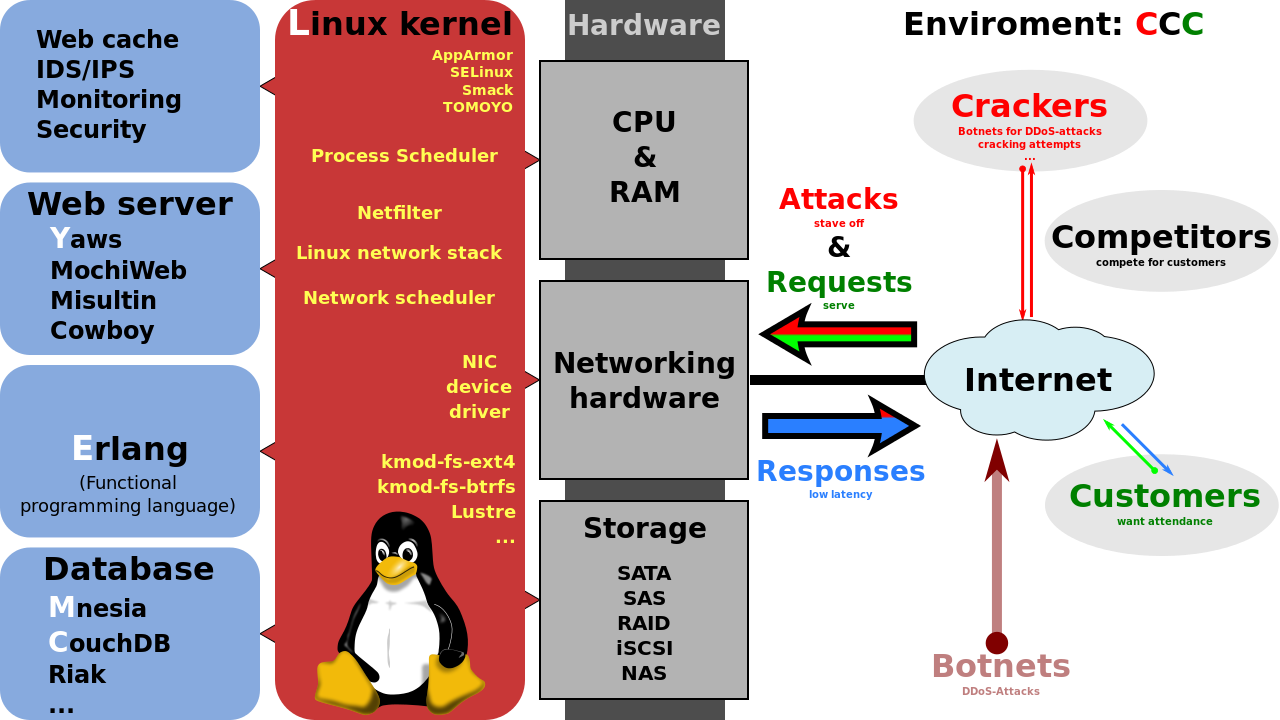
\includegraphics[scale=0.5]{LYME.png}
\caption{LYME}
\end{figure}




\section{Linux}


\begin{lstlisting}[language=bash]

\end{lstlisting}




\begin{lstlisting}[language=bash]

\end{lstlisting}


\section{Yaws}


\begin{lstlisting}[language=bash]

\end{lstlisting}




\begin{lstlisting}[language=bash]

\end{lstlisting}


\section{Mnesia}



\begin{lstlisting}[language=bash]

\end{lstlisting}



\begin{lstlisting}[language=bash]

\end{lstlisting}



\begin{lstlisting}[language=bash]

\end{lstlisting}


\section{Erlang}


\begin{lstlisting}[language=bash]

\end{lstlisting}




\begin{lstlisting}[language=bash]

\end{lstlisting}


\chapter{LAPP}



\section{Linux}


\begin{lstlisting}[language=bash]

\end{lstlisting}




\begin{lstlisting}[language=bash]

\end{lstlisting}


\section{Apache}


\begin{lstlisting}[language=bash]

\end{lstlisting}





\begin{lstlisting}[language=bash]

\end{lstlisting}

\section{PHP}


\begin{lstlisting}[language=bash]

\end{lstlisting}




\begin{lstlisting}[language=bash]

\end{lstlisting}


\section{PostgreSQL}


\begin{lstlisting}[language=bash]

\end{lstlisting}




\begin{lstlisting}[language=bash]

\end{lstlisting}




\begin{lstlisting}[language=bash]

\end{lstlisting}


\chapter{WAMP}



\section{Windows}


\begin{lstlisting}[language=bash]

\end{lstlisting}




\begin{lstlisting}[language=bash]

\end{lstlisting}



\section{Apache}


\begin{lstlisting}[language=bash]

\end{lstlisting}



\begin{lstlisting}[language=bash]

\end{lstlisting}


\section{MySQL}


\begin{lstlisting}[language=bash]

\end{lstlisting}




\begin{lstlisting}[language=bash]

\end{lstlisting}


\section{PHP}


\begin{lstlisting}[language=bash]

\end{lstlisting}




\begin{lstlisting}[language=bash]

\end{lstlisting}




\begin{lstlisting}[language=bash]

\end{lstlisting}

\chapter{LAMJ}



\section{Linux}



\begin{lstlisting}[language=bash]

\end{lstlisting}





\begin{lstlisting}[language=bash]

\end{lstlisting}

\section{Apache}


\begin{lstlisting}[language=bash]

\end{lstlisting}




\begin{lstlisting}[language=bash]

\end{lstlisting}


\section{MySQL}


\begin{lstlisting}[language=bash]

\end{lstlisting}




\begin{lstlisting}[language=bash]

\end{lstlisting}


\section{Java}



\begin{lstlisting}[language=bash]

\end{lstlisting}




\begin{lstlisting}[language=bash]

\end{lstlisting}


\chapter{BAMP}



\section{BSD}


\begin{lstlisting}[language=bash]

\end{lstlisting}





\begin{lstlisting}[language=bash]

\end{lstlisting}



\begin{lstlisting}[language=bash]

\end{lstlisting}



\section{Apache}




\begin{lstlisting}[language=bash]

\end{lstlisting}



\begin{lstlisting}[language=bash]

\end{lstlisting}



\section{MySQL}


\begin{lstlisting}[language=bash]

\end{lstlisting}



\begin{lstlisting}[language=bash]

\end{lstlisting}



\section{PHP}


\begin{lstlisting}[language=bash]

\end{lstlisting}



\begin{lstlisting}[language=bash]

\end{lstlisting}


\chapter{WIMP}



\section{Windows}



\begin{lstlisting}[language=bash]

\end{lstlisting}



\begin{lstlisting}[language=bash]

\end{lstlisting}


\section{IIS}



\begin{lstlisting}[language=bash]

\end{lstlisting}



\begin{lstlisting}[language=bash]

\end{lstlisting}


\section{MySQL}



\begin{lstlisting}[language=bash]

\end{lstlisting}



\begin{lstlisting}[language=bash]

\end{lstlisting}


\section{PHP}



\begin{lstlisting}[language=bash]

\end{lstlisting}



\begin{lstlisting}[language=bash]

\end{lstlisting}





\begin{lstlisting}[language=bash]

\end{lstlisting}



\begin{lstlisting}[language=bash]

\end{lstlisting}





\begin{lstlisting}[language=bash]

\end{lstlisting}



\begin{lstlisting}[language=bash]

\end{lstlisting}






\begin{lstlisting}[language=bash]

\end{lstlisting}



\begin{lstlisting}[language=bash]

\end{lstlisting}





\begin{lstlisting}[language=bash]

\end{lstlisting}



\begin{lstlisting}[language=bash]

\end{lstlisting}






\begin{lstlisting}[language=bash]

\end{lstlisting}



\begin{lstlisting}[language=bash]

\end{lstlisting}





\begin{lstlisting}[language=bash]

\end{lstlisting}



\begin{lstlisting}[language=bash]

\end{lstlisting}





\begin{lstlisting}[language=bash]

\end{lstlisting}



\begin{lstlisting}[language=bash]

\end{lstlisting}





\begin{lstlisting}[language=bash]

\end{lstlisting}



\begin{lstlisting}[language=bash]

\end{lstlisting}

\part{Configuration}


\chapter{Overview}





\chapter{httpd.conf}



\begin{lstlisting}[language=bash]

\end{lstlisting}




\begin{lstlisting}[language=bash]

\end{lstlisting}




\begin{lstlisting}[language=bash]

\end{lstlisting}




\begin{lstlisting}[language=bash]

\end{lstlisting}





\begin{lstlisting}[language=bash]

\end{lstlisting}




\begin{lstlisting}[language=bash]

\end{lstlisting}




\begin{lstlisting}[language=bash]

\end{lstlisting}




\begin{lstlisting}[language=bash]

\end{lstlisting}





\begin{lstlisting}[language=bash]

\end{lstlisting}




\begin{lstlisting}[language=bash]

\end{lstlisting}




\begin{lstlisting}[language=bash]

\end{lstlisting}




\begin{lstlisting}[language=bash]

\end{lstlisting}





\begin{lstlisting}[language=bash]

\end{lstlisting}




\begin{lstlisting}[language=bash]

\end{lstlisting}




\begin{lstlisting}[language=bash]

\end{lstlisting}




\begin{lstlisting}[language=bash]

\end{lstlisting}





\begin{lstlisting}[language=bash]

\end{lstlisting}




\begin{lstlisting}[language=bash]

\end{lstlisting}




\begin{lstlisting}[language=bash]

\end{lstlisting}




\begin{lstlisting}[language=bash]

\end{lstlisting}





\begin{lstlisting}[language=bash]

\end{lstlisting}




\begin{lstlisting}[language=bash]

\end{lstlisting}




\begin{lstlisting}[language=bash]

\end{lstlisting}




\begin{lstlisting}[language=bash]

\end{lstlisting}





\begin{lstlisting}[language=bash]

\end{lstlisting}




\begin{lstlisting}[language=bash]

\end{lstlisting}




\begin{lstlisting}[language=bash]

\end{lstlisting}




\begin{lstlisting}[language=bash]

\end{lstlisting}





\begin{lstlisting}[language=bash]

\end{lstlisting}




\begin{lstlisting}[language=bash]

\end{lstlisting}




\begin{lstlisting}[language=bash]

\end{lstlisting}




\begin{lstlisting}[language=bash]

\end{lstlisting}





\begin{lstlisting}[language=bash]

\end{lstlisting}




\begin{lstlisting}[language=bash]

\end{lstlisting}




\begin{lstlisting}[language=bash]

\end{lstlisting}




\begin{lstlisting}[language=bash]

\end{lstlisting}





\begin{lstlisting}[language=bash]

\end{lstlisting}




\begin{lstlisting}[language=bash]

\end{lstlisting}




\begin{lstlisting}[language=bash]

\end{lstlisting}




\begin{lstlisting}[language=bash]

\end{lstlisting}


\chapter{nginx.conf}

默认情况下,Nginx的配置文件nginx.conf位于Nginx安装目录的conf子目录下,在编译前的configure阶段可以通过\texttt{--conf-path}参数进行指定。

nginx.conf的结构可以划分为下面的部分:

\begin{lstlisting}[language=bash]
...
events
{
  ...
}

http
{
  ...
  server
  {
    ...
  }
  
  server
  {
    ...
  }
...
}


\end{lstlisting}

\section{user}



\begin{compactitem}
\item 如果只指定用户,可以设置:

\begin{lstlisting}[language=bash]
#user nginx;
\end{lstlisting}

\item 如果同时指定用户和用户组,可以设置:

\begin{lstlisting}[language=bash]
#user nginx nginx;
\end{lstlisting}
\end{compactitem}


\section{worker\_process}

worker进程数一般等于CPU的总核数或总核数的两倍。

\begin{lstlisting}[language=bash]
worker_process 8;
\end{lstlisting}


\section{error\_log}

除了可以指定错误日志的存放路径之外,还可以设置错误日志记录级别。

\begin{compactitem}
\item debug
\item info
\item notice
\item warn
\item error
\item crit
\end{compactitem}




\begin{lstlisting}[language=bash]
#error_log logs/error.log;
#error_log logs/error.log notice;
#error_log logs/error.log info;
\end{lstlisting}




\section{pid}


pid文件的存放路径也可以在nginx.conf中指定。

\begin{lstlisting}[language=bash]
pid /var/run/nginx.pid;
\end{lstlisting}

\section{worker\_rlimit\_nofile}

worker\_rlimit\_nofile可以指定文件描述符数量(例如51200)。

\begin{lstlisting}[language=bash]
worker_rlimit_nofile 51200;
\end{lstlisting}


\section{events}

在events部分,可以指定Nginx使用的网络IO模型(例如Linux推荐使用epoll模型,FreeBSD系统则推荐使用kqueue模型)。



\begin{lstlisting}[language=bash]
events
{
  use epoll;
}
\end{lstlisting}

另外,在events部分还可以设置允许的连接数,例如:


\begin{lstlisting}[language=bash]
events
{
  use epoll;
  worker_connections 51200;
}
\end{lstlisting}


\section{http}




\begin{lstlisting}[language=bash]
http
{
  include mime.types;
  default_type application/octet-stream;
}
\end{lstlisting}

\subsection{charset}

对于国际化网站,不能随意设置字符集,而是让开发者在HTML代码中通过<meta>标签设置。



\begin{lstlisting}[language=bash]
http
{
  include mime.types;
  default_type application/octet-stream;
  #charset gb2312;
  
  server_names_hash_bucket_size 128;
  client_header_buffer_size 32k;
  large_client_header_buffers 4 32k;
}
\end{lstlisting}


\subsection{client\_max\_body\_size}

在nginx.conf中可以设置客户端能够上传的文件大小。


\begin{lstlisting}[language=bash]
http
{
  include mime.types;
  default_type application/octet-stream;
  #charset gb2312;
  
  server_names_hash_bucket_size 128;
  client_header_buffer_size 32k;
  large_client_header_buffers 4 32k;
  
  client_max_body_size 8m;
  sendfile on;
  tcp_nopush on;
  
  #keepalive_timeout 60;
  
  tcp_nodelay on;
}
\end{lstlisting}


\subsection{fastcgi\_*}

FastCGI是语言无关的、可伸缩架构的CGI开放扩展,其主要作用是将CGI解释器进程保持在内存中来获得较高的性能,从而解决CGI解释器反复加载而导致性能低下的问题。

FastCGI可以让CGI解释器驻留在内存中,并接受FPM(FastCGI进程管理器)的调度,从而实现良好的性能、伸缩性和Fail-Over等特性。

下面说明FastCGI的工作原理:

\begin{compactitem}
\item FPM自身初始化,启动多个CGI解释器进程(即多个php-cgi进程)并等待来自Nginx进程的连接,而且在启动CGI解释器时可以配置是否以TCP或UNIX套接字方式启动。

\item 客户端请求被传递到Nginx进程时,如果不是静态文件请求则会被Nginx进程以TCP协议或UNIX套接字方式转发到FastCGI主进程,然后FastCGI主进程会选择并连接到一个CGI解释器(子进程),Nginx进程会将CGI环境变量和标准输入发送到FastCGI子进程php-cgi。

\item FastCGI子进程完成处理后将标准输出和错误信息从同一连接返回给Nginx进程。

\item FastCGI子进程关闭连接时,说明请求被处理完成,然后FastCGI子进程会继续等待并处理来自FPM调度的下一个连接。

如果是在一般的普通CGI模式中,CGI子进程php-cgi会就此结束,因此普通的CGI模式在处理每一个请求时都必须重新解析php.ini、重新载入全部扩展并重新初始化全部数据结构,FastCGI的引入使得上述过程只需在进程启动时处理一次,同时也使得数据库持久连接(persisten connection)可以正常工作。
\end{compactitem}



\begin{lstlisting}[language=bash]
http
{
  include mime.types;
  default_type application/octet-stream;
  #charset gb2312;
  
  server_names_hash_bucket_size 128;
  client_header_buffer_size 32k;
  large_client_header_buffers 4 32k;
  
  client_max_body_size 8m;
  sendfile on;
  tcp_nopush on;
  
  #keepalive_timeout 60;
  
  tcp_nodelay on;
  
  fastcgi_connect_timeout 300;
  fastcgi_send_timeout 300;
  fastcgi_read_timeout 300;
  fastcgi_buffer_size 64k;
  fastcgi_buffers 4 64k;
  fastcgi_busy_buffers_size 128k;
  fastcgi_temp_file_write_size 128k;
}
\end{lstlisting}



\subsection{gzip\_*}


gzip压缩


\begin{lstlisting}[language=bash]
http
{
  include mime.types;
  default_type application/octet-stream;
  #charset gb2312;
  
  server_names_hash_bucket_size 128;
  client_header_buffer_size 32k;
  large_client_header_buffers 4 32k;
  
  client_max_body_size 8m;
  sendfile on;
  tcp_nopush on;
  
  #keepalive_timeout 60;
  
  tcp_nodelay on;
  
  fastcgi_connect_timeout 300;
  fastcgi_send_timeout 300;
  fastcgi_read_timeout 300;
  fastcgi_buffer_size 64k;
  fastcgi_buffers 4 64k;
  fastcgi_busy_buffers_size 128k;
  fastcgi_temp_file_write_size 128k;
  
  gzip on;
  gzip_min_length 1k;
  gzip_buffers 4 16k;
  gzip_http_version 1.1;
  gzip_comp_level 2;
  gzip_types text/plain application/x-javascript text/css application/xml;
  gzip_vary on;
}
\end{lstlisting}

\subsection{limit\_zone}



\begin{lstlisting}[language=bash]
#limit_zone crawler $binary_remote_addr 10m;
\end{lstlisting}




\begin{lstlisting}[language=bash]

\end{lstlisting}




\begin{lstlisting}[language=bash]

\end{lstlisting}





\begin{lstlisting}[language=bash]

\end{lstlisting}




\begin{lstlisting}[language=bash]

\end{lstlisting}




\begin{lstlisting}[language=bash]

\end{lstlisting}




\begin{lstlisting}[language=bash]

\end{lstlisting}





\begin{lstlisting}[language=bash]

\end{lstlisting}




\begin{lstlisting}[language=bash]

\end{lstlisting}




\begin{lstlisting}[language=bash]

\end{lstlisting}




\begin{lstlisting}[language=bash]

\end{lstlisting}





\begin{lstlisting}[language=bash]

\end{lstlisting}




\begin{lstlisting}[language=bash]

\end{lstlisting}




\begin{lstlisting}[language=bash]

\end{lstlisting}




\begin{lstlisting}[language=bash]

\end{lstlisting}





\begin{lstlisting}[language=bash]

\end{lstlisting}




\begin{lstlisting}[language=bash]

\end{lstlisting}




\begin{lstlisting}[language=bash]

\end{lstlisting}




\begin{lstlisting}[language=bash]

\end{lstlisting}





\begin{lstlisting}[language=bash]

\end{lstlisting}




\begin{lstlisting}[language=bash]

\end{lstlisting}




\begin{lstlisting}[language=bash]

\end{lstlisting}




\begin{lstlisting}[language=bash]

\end{lstlisting}





\begin{lstlisting}[language=bash]

\end{lstlisting}




\begin{lstlisting}[language=bash]

\end{lstlisting}




\begin{lstlisting}[language=bash]

\end{lstlisting}




\begin{lstlisting}[language=bash]

\end{lstlisting}


\subsection{server}




Nginx的server块基本等同于Apache的virtual hosts,因此可以通过server块设置来配置Nginx虚拟主机。



\begin{lstlisting}[language=bash]
server
{
  listen 80;
  server_name www.youdomain.com yourdomain.com;
  index index.html index.htm;
  root /etc/nginx/html;
  
  #limit_conn crawler 20;
  
  location ~ .*\.(gif|jpg|jpeg|png|bmp|swf)$
  {
    expires 30d;
  }
  
  location ~ .*\.(js|css)?$
  {
    expires 1h;
  }
  
  log_format access '$remote_addr - $remote_user [$time_local] "$request" $status $body_bytes_sent "$http_referer" "$http_user_agent" $http_x_forwarded_for';
  access_log /var/log/nginx/access.log access;  
}
\end{lstlisting}


默认情况下,Nginx只能处理静态网页,因此需要设置Nginx对PHP等动态网页的支持。



\begin{lstlisting}[language=bash]
server {
    listen       80;
    server_name  server-ip;
 
    root   /usr/share/nginx/html;
    index index.php index.html index.htm;
 
    location / {
        try_files $uri $uri/ =404;
    }
    error_page 404 /404.html;
    error_page 500 502 503 504 /50x.html;
    location = /50x.html {
        root /usr/share/nginx/html;
    }
 
    location ~ \.php$ {
        try_files $uri =404;
        fastcgi_pass unix:/var/run/php-fpm/php-fpm.sock;
        fastcgi_index index.php;
        fastcgi_param SCRIPT_FILENAME $document_root$fastcgi_script_name;
        include fastcgi_params;
    }
}
\end{lstlisting}

在设置Nginx的虚拟主机以及对PHP的支持后,同样需要重启Nginx服务器来使修改生效。

\begin{lstlisting}[language=bash]
$ sudo systemctl restart nginx.service
\end{lstlisting}





\begin{lstlisting}[language=bash]

\end{lstlisting}



\section{virtual host}

虚拟主机(virtual host)技术基于特殊的软硬件技术来将物理主机划分为多台“虚拟”的主机,而且每台虚拟主机都可以是一个独立的网站,并且可以具有独立的域名以及完整的Internet服务器功能(例如WWW、FTP和Email等)。

同一台物理主机上虚拟主机之间是完全独立的,从网站的访问者看来,每一台虚拟主机和一台独立的物理主机完全一样。

Nginx和Apache等可以通过虚拟主机来为每一个要运行的网站提供一台单独的“服务器”,而且虚拟主机之间共享一组Nginx进程,这样就可以在同一台物理主机上的同一组Nginx进程上运行多个网站。

首先,Nginx配置文件中的一个最简化的虚拟主机配置结构如下:

\begin{lstlisting}[language=bash]
http
{
	server
	{
		listen  80;
		server_name  _ *;
		access_log /var/log/nginx/access.log combined;
		location /
		{
			index index.html index.htm;
			root /etc/nginx/html;
		}
	}
}
\end{lstlisting}


其次,用户可以基于IP来配置虚拟主机,也可以基于域名配置虚拟主机,还可以基于端口来配置虚拟主机。

\subsection{Domain}


在配置基于域名的虚拟主机时,只需要在DNS服务器上将每个域名对应的主机名映射到正确的IP地址,然后配置Nginx服务器来识别不同的主机名。


基于域名的虚拟主机的好处在于可以让多个虚拟主机共享同一个IP地址,从而解决IP地址不足的问题。

\begin{compactitem}
\item index项指定了默认的首页文件,顺序从左到右,如果找不到第一个文件,则查找第二个文件作为首页,依次类推。
\item server\_name项指定了对域名的访问规则,如果找不到精确匹配的域名,则查找支持泛域名匹配的虚拟主机,并由它来处理请求。
\end{compactitem}

\begin{lstlisting}[language=bash]
user nginx;
worker_processes 8;
error_log /var/nginx/logs/error.log;
error_log /var/nginx/logs/error.log notice;
error_log /var/nginx/logs/error.log info;

pid /var/run/nginx.pid;

worker_rlimit_nofile 51200;

events
{
	worker_connections 1024;
}

http
{
	include mime.types;
	default_type application/octet-stream;
	
	#log_format  main  '$remote_addr - $remote_user [$time_local] "$request" '
	#	'$status $body_bytes_sent "$http_referer" '
	#	'"$http_user_agent" "$http_x_forwarded_for"';
	
	#access_log /var/log/nginx/access.log main;
	
	send_file on;
	#tcp_nopush on;
	
	keepalive_timeout 65;	
	gzip on;
	gzip_min_length 1100;
	gzip_buffers 4 8k;
	gzip_types text/plain text/css application/x-javascript;
	gzip_com_level 4;
	
	server_tokens off;
	underscores_in_headers on;
	server
	{
		listen 80;
		server_name test.com;
		
		#charset koi8-r;
		#access_log /var/log/nginx/access.log main;
		#underscores_in_headers on;
		
		location /
		{
			root /etc/nginx/html;
			index index.html index.htm index.php;
			if(!-e $request_filename){
				rewrite ^/(.*)$ /index.php/$1 last;
			}
		}
		
		#error_page 404 /404.htm;
		# redirect server error pages to the static page /50x.html
		error_page 500 502 503 504 /50x.html;
		location = /50x.html {
			root html;
		}
		
		# proxy the PHP scripts to Apache listening on 127.0.0.1:80
		#
		#location ~ \.php$ {
		#	proxy_pass http://127.0.0.1;
		#}
		
		# pass the PHP scripts to FastCGI server listening on 127.0.0.1:9000
		#
		location ~ \.php {
			root /etc/nginx/html;
			fastcgi_pass 127.0.0.1:9000;
			fastcgi_index index.php;
			#fastcgi_param SCRIPT_FILENAME /scripts$fastcgi_script_name;
			fastcgi_param SCRIPT_FILENAME $document_root$fastcgi_script_name;
			send_timeout 60;
			include fastcgi_params;
		}
		
		# deny access to .htaccess files, if Apache's document root
		# concurs with nginx's one
		# 
		#location ~ /\.ht {
		#	deny all;
		#}
	}
}
\end{lstlisting}

不同的虚拟主机可以使用不同的日志文件来记录访问日志。


\subsection{IP Addr}

Linux和FreeBSD等操作系统都允许添加IP别名,IP别名就是在同一块物理网卡上绑定多个IP地址,这样就可以在使用单一网卡的同一台服务器上运行多个基于IP的虚拟主机。

设置IP别名就是使用网络配置工具ifconfig和route等工具来配置系统上的网络接口来让其监听额外的IP地址。



\begin{lstlisting}[language=bash]
# ifconfig
eth0      Link encap:Ethernet  HWaddr 00:16:3E:00:79:90  
          inet addr:10.168.8.66  Bcast:10.168.15.255  Mask:255.255.248.0
          UP BROADCAST RUNNING MULTICAST  MTU:1500  Metric:1
          RX packets:31996368 errors:0 dropped:0 overruns:0 frame:0
          TX packets:145210 errors:0 dropped:0 overruns:0 carrier:0
          collisions:0 txqueuelen:1000 
          RX bytes:1351005648 (1.2 GiB)  TX bytes:12348718 (11.7 MiB)
          Interrupt:145 

eth1      Link encap:Ethernet  HWaddr 00:16:3E:00:7C:0C  
          inet addr:121.40.126.146  Bcast:121.40.127.255  Mask:255.255.252.0
          UP BROADCAST RUNNING MULTICAST  MTU:1500  Metric:1
          RX packets:327532453 errors:0 dropped:0 overruns:0 frame:0
          TX packets:1874590 errors:0 dropped:0 overruns:0 carrier:0
          collisions:0 txqueuelen:1000 
          RX bytes:14984090397 (13.9 GiB)  TX bytes:516587686 (492.6 MiB)
          Interrupt:144 

lo        Link encap:Local Loopback  
          inet addr:127.0.0.1  Mask:255.0.0.0
          UP LOOPBACK RUNNING  MTU:65536  Metric:1
          RX packets:463875002 errors:0 dropped:0 overruns:0 frame:0
          TX packets:463875002 errors:0 dropped:0 overruns:0 carrier:0
          collisions:0 txqueuelen:0 
          RX bytes:222067269546 (206.8 GiB)  TX bytes:222067269546 (206.8 GiB)
\end{lstlisting}

其中,lo(local loopback,本地回环)代表本地虚拟接口,默认被看作是永远不会宕掉的接口,其主要作用有两个:

\begin{compactitem}
\item 测试本机的网络配置,例如\texttt{ping 127.0.0.1}测试本地网卡和网络协议安装是否成功。
\item 某些server/client程序在运行时需要请求server端的资源,如果server的IP地址设置为127.0.0.1则可以请求本地资源。
\end{compactitem}

下面的命令在网卡设备eth0上添加两个IP别名(192.168.8.43和192.168.8.44):


\begin{lstlisting}[language=bash]
# /sbin/ifconfig eth0:1 192.168.8.43 broadcast 192.168.8.255 netmask 255.255.255.0 up
# /sbin/route add -host 192.168.8.43 dev eth0:1

# /sbin/ifconfig eth0:2 192.168.8.44 broadcast 192.168.8.255 netmask 255.255.255.0 up
# /sbin/route add -host 192.168.8.44 dev eth0:2
\end{lstlisting}

为了防止上述配置在重启后失效,可以将其加入到/etc/rc.local,这样系统重启时就会自动执行上述命令来设置IP别名。



\begin{lstlisting}[language=bash]
# vim /etc/rc.local
/sbin/ifconfig eth0:1 192.168.8.43 broadcast 192.168.8.255 netmask 255.255.255.0 up
/sbin/route add -host 192.168.8.43 dev eth0:1
/sbin/ifconfig eth0:2 192.168.8.44 broadcast 192.168.8.255 netmask 255.255.255.0 up
/sbin/route add -host 192.168.8.44 dev eth0:2
\end{lstlisting}

实际上,无论是通过IP别名在一台服务器上配置多个IP地址,还是通过多个网卡来配置多个IP别名,Nginx都可以支持配置成基于IP的虚拟主机。




\begin{lstlisting}[language=bash]
http
{
	# vhost0
	server
	{
		listen 192.168.8.43:80;
		server_name 192.168.8.43;
		access_log /var/log/nginx/vhost0.log combined;
		location /
		{
			index index.html index.htm;
			root /etc/nginx/vhost0;
		}
	}
	
	#vhost2
	server
	{
		listen 192.168.8.44:80;
		server_name 192.168.8.44;
		access_log /var/log/nginx/vhost1.log combined;
		location /
		{
			index index.html index.htm;
			root /etc/nginx/vhost1;
		}
	}
}
\end{lstlisting}

注意,监听的IP和端口也可以不指定IP地址,只指定端口。例如,\texttt{listen 80;}代表监听该服务器上所有IP的80端口,可以通过server\_name区分不同的虚拟主机。


\begin{lstlisting}[language=bash]

\end{lstlisting}




\begin{lstlisting}[language=bash]

\end{lstlisting}





\begin{lstlisting}[language=bash]

\end{lstlisting}


\section{access\_log}


与Nginx的日志相关的指令主要是log\_format和access\_log,其中:

\begin{compactitem}
\item log\_format用来设置日志的格式;
\item access\_log用来指定日志文件的存放路径、格式和缓存大小。
\end{compactitem}


log\_format和access\_log配置项的位置可以在\texttt{http\{...\}}内部,也可以在虚拟主机内部(即\texttt{server\{...\}})。


\subsection{log\_format}


log\_format指令用来设置日志的记录格式,其语法如下:


\begin{lstlisting}[language=bash]
Syntax:	log_format name string ...;
Default:	log_format combined "...";
Context:	http
\end{lstlisting}


\begin{compactitem}
\item name表示定义的格式名称;
\item format表示定义的格式样式。
\end{compactitem}

log\_format的默认的无需设置的combined日志格式设置,相当于Apache的combined日志格式,其具体参数如下:



\begin{lstlisting}[language=bash]
log_format combined '$remote_addr - $remote_user [$time_local] '
                    '"$request" $status $body_bytes_sent '
                    '"$http_referer" "$http_user_agent"';
\end{lstlisting}


用户可以自定义日志的记录格式,只要log\_format指令设置的name名称在nginx.conf中不重复即可。

在生产环境中,Nginx服务器通常位于负载均衡设备、squid和Nginx反向代理之后,那么就无法获得客户端的真实IP地址。

反向代理作为客户端和Nginx服务器之间的中间层导致Nginx服务器无法直接获得客户端的IP,而且\$remote\_addr变量拿到的也只是反向代理服务器的IP地址,但是可以在反向代理服务器的转发请求的HTTP头信息中增加X-Forwarded-For信息,这样就可以记录原有的客户端IP地址和原有的客户端请求的服务器地址。

下面在log\_format指令中设置日志格式,并且让日志记录X-Forwarded-For信息中的IP地址(即客户端的真实IP地址)。

\begin{lstlisting}[language=bash]
log_format mylogformat '$http_x_forwarded_for - $remote_user [$time_local] '
			'"$request" $status $body_bytes_sent '
			'"$http_referer" "$http_user_agent"';
\end{lstlisting}

\begin{compactitem}
\item 变量\texttt{\$remote\_addr}记录IP地址;
\item 变量\texttt{\$http\_x\_forwarded\_for}记录IP地址;
\item 变量\texttt{\$remote\_user}记录远程客户端用户名称;
\item 变量\texttt{\$time\_local}记录访问时间和时区;
\item 变量\texttt{\$request}记录请求URL和HTTP协议;
\item 变量\texttt{\$status}记录请求状态,例如200代表请求成功;
\item 变量\texttt{\$body\_bytes\_sent}记录发送给客户端的文件主体内容大小;
\item 变量\texttt{\$http\_referer}记录跳转过来之前的页面链接;
\item 变量\texttt{\$http\_user\_agent}记录客户端浏览器的相关信息。
\end{compactitem}



\subsection{access\_log}


access\_log指令指定日志文件的存放路径,其语法如下:



\begin{lstlisting}[language=bash]
Syntax:	access_log path [format [buffer=size [flush=time]] [if=condition]];
access_log path format gzip[=level] [buffer=size] [flush=time] [if=condition];
access_log syslog:server=address[,parameter=value] [format [if=condition]];
access_log off;
Default:	access_log logs/access.log combined;
Context:	http, server, location, if in location, limit_except
\end{lstlisting}

\begin{compactitem}
\item path表示日志文件的存放路径;
\item format表示使用log\_format指令设置的日志格式的名称;
\item buffer表示设置的内存缓冲区的大小(例如\texttt{buffer=32k})。
\end{compactitem}

\begin{compactenum}
\item 如果不需要记录日志,可以关闭日志记录。

\begin{lstlisting}[language=bash]
access_log off;
\end{lstlisting}

\item 如果需要默认的combined格式的日志记录,可以设置:

\begin{lstlisting}[language=bash]
access_log /var/log/nginx/access.log
\end{lstlisting}

或

\begin{lstlisting}[language=bash]
access_log /var/log/nginx/access.log combined;
\end{lstlisting}

\item 如果需要使用自定义格式的日志记录,可以设置:

\begin{lstlisting}[language=bash]
log_format mylogformat '$http_x_forwarded_for - $remote_user [$time_local] '
			'"$request" $status $body_bytes_sent '
			'"$http_referer" "$http_user_agent"';
access_log /var/log/nginx/access.log mylogformat buffer=32k;
\end{lstlisting}


\end{compactenum}

另外,Nginx允许在access\_log指令中的日志文件路径中包含变量,例如:


\begin{lstlisting}[language=bash]
access_log /var/log/nginx/$server_name.log combined;
\end{lstlisting}

不过,在日志文件路径中包含变量有一定的副作用。

\begin{compactitem}
\item Nginx进程设置的用户和用户组必须有对该路径创建文件的权限,否则需要用户自己手动创建并修改拥有者信息。

\item 缓存无法被使用。

\item 对于每一条日志记录,日志文件都将先打开文件,再写入日志记录,然后关闭文件。

\end{compactitem}


日志文件的增长可能会影响到服务器效率,而且日志太大也不方便进行分析计算,因此需要对日志文件进行定时切割。

根据需求,可以按月切割、按天切割、按小时切割等方式来处理日志。

和Apache不同,Nginx不支持使用cronolog来进行日志轮转,因此用户需要采用kill命令并指定USR1\footnote{USR1系统信号指示Nginx重新生成新的日志文件(在切割日志时用途较大)。}系统信号来手动进行日志文件的切割。

\begin{lstlisting}[language=bash]
# mv /var/log/nginx/access.log /var/log/nginx/xxxx-xx-xx.log
# kill -USR1 nginx_master_process_id
\end{lstlisting}


\begin{compactitem}
\item 如果nginx.conf中指定了pid文件的存放路径,那么可以执行:

\begin{lstlisting}[language=bash]
# mv /var/log/nginx/access.log /var/log/nginx/xxxx-xx-xx.log
# kill -USR1 `cat /var/run/nginx.pid`
\end{lstlisting}

\item 如果需要每天定时切割日志,可以借助crontab来执行定时任务,并且按年-月-日格式来存放日志。

\begin{lstlisting}[language=bash]
# cat cut_nginx_log.sh
#!/bin/bash
# 日志存放路径
logs_path="/var/log/";

mkdir -p ${logs_path}$(date -d "yesterday" +"%Y")/$(date -d "yesterday" +"%m"/
mv ${logs_path}access.log ${logs_path}$(date -d "yesterday" +"%Y")/$(date -d "yesterday" +"%m")/access_$(date -d "yesterday" +"%Y%m%d").log
kill -USR1 `cat /var/run/nginx.pid`
\end{lstlisting}

\end{compactitem}

下面配置crontab在每天的凌晨00:00定时执行上述脚本:

\begin{lstlisting}[language=bash]
# crontab -e
00 00 * * * /bin/bash /usr/sbin/cut_nginx_log.sh
\end{lstlisting}



\subsection{open\_log\_file\_cache}



为了提高包含变量的日志文件存放路径的性能,必须使用open\_log\_file\_cache指令设置被使用的日志文件描述符缓存。

实际上,open\_log\_file\_cache指令主要用来设置包含变量的日志路径的文件描述符缓存,其语法格式如下:


\begin{lstlisting}[language=bash]
Syntax: open_log_file_cache max=N [inactive=time] [min_uses=N] [valid=time];
open_log_file_cache off;
Default: open_log_file_cache off;
Context:	http, server, location
\end{lstlisting}


默认情况下,open\_log\_file\_cache指令是禁止的,等同于:

\begin{lstlisting}[language=bash]
open\_log\_file\_cache off;
\end{lstlisting}


\begin{compactitem}
\item max:设置缓存中的最大文件描述符数量。

如果超过设置的最大文件描述符数量,则采用LRU(Least Recently Used)算法清除“较不常使用的文件描述符”,当内存缓冲区剩余的可用空间不够时,缓冲区尽可能地先保留使用者最常使用的数据,将最近未使用的数据移出内存,从而腾出空间来加载另外的数据。

\item inactive:设置文件描述符的最长不被使用间隔,否则自动删除该文件描述符,默认时间为10秒钟。

\item min\_uses:在参数inactive指定的时间范围内,如果日志文件超过被使用的次数,则将该日志文件的描述符记入缓存,默认次数为1。

\item valid:设置检查变量指定的日志文件路径与文件名是否仍然存在的时间间隔,默认为60秒。

\item off:禁止使用缓存。

\end{compactitem}




\begin{lstlisting}[language=bash]
open_log_file_cache max=1000 inactive=20s min_uses=2 valid=1m;
\end{lstlisting}




\begin{lstlisting}[language=bash]

\end{lstlisting}



\section{gzip}


gzip(GNU-ZIP)技术需要浏览器和服务器同时支持,这样就可以在服务器端对页面进行压缩,然后将页面传送到浏览器时解压缩并进行解析,从而提高页面的展现速度。


Nginx提供的压缩输出由一组位于\texttt{http\{...\}}内部的gzip指令实现。


\begin{lstlisting}[language=bash]
gzip on;
gzip_min_length 1k;
gzip_buffers 4 16k;
gzip_http_version 1.1;
gzip_comp_level 2;
gzip_types text/plain application/x-javascript text/css application/xml;
gzip_vary on;
\end{lstlisting}

\section{autoindex}


Apache和Nginx都可以实现自动列目录设置,前提条件是当前目录下不存在用index指令设置的默认首页文件。例如,如果需要在虚拟主机上的\texttt{location / \{...\}}目录控制中配置自动列目录,可以设置:



\begin{lstlisting}[language=bash]
location /
{
  autoindex on;
}
\end{lstlisting}

另外,和自动列目录相关的命令分别是autoindex\_exact\_size和autoindex\_localtime。

\subsection{autoindex\_exact\_size}

autoindex\_exact\_size用于设定索引时文件大小的单位(B、KB、MB或GB)。


\begin{lstlisting}[language=bash]
autoindex_exact_size [on|off]
\end{lstlisting}

\subsection{autoindex\_localtime}

autoindex\_localtime可以设置是否开启本地时间来显示文件时间,默认为关(GMT时间)。

\begin{lstlisting}[language=bash]
autoindex_localtime [on|off]
\end{lstlisting}




\begin{lstlisting}[language=bash]

\end{lstlisting}


\section{expires}


浏览器缓存(browser caching)可以在用户磁盘上对最近请求过的文档进行存储,这样当访问者再次请求该页面时,浏览器就可以从本地磁盘加载文档,从而加速浏览效果。

浏览器缓存可以节约网络资源,提高网络效率,通过Nginx的expires指令可以在Header中输出对应的浏览器缓存指令(例如Expires和Cache-Control)。


expires指令的作用域包括http、server和location等。

\begin{lstlisting}[language=bash]
Syntax:	expires [modified] time;
expires epoch | max | off;
Default:	expires off;
Context:	http, server, location, if in location
\end{lstlisting}


默认情况下,expires指令是关闭的,表示不修改“Expires”和“Cache-Control”的值。

expires指令可以控制HTTP应答中的“Expires”和“Cache-Control”来指定页面缓存,其中可以在time中设置正值或负值来影响“Expires”的值\footnote{具体来说,Expires的值通过在当前系统时间上加上设定的time值来获得。}。

\begin{compactitem}
\item epoch指定“Expires”的值为1 January, 1970, 00:00:01 GMT。
\item max指定“Expires”的值为31 December, 2037, 23:59:59 GMT,并指定“Cache-Control”的值为10年。
\end{compactitem}

如果指定expires为-1,那么“Expires”的值为服务器当前时间减1秒,即永远过期。

Cache-Control的值由用户指定的时间来决定,例如:

\begin{compactitem}
\item 负数:\texttt{Cache-Control:no-cache}
\item 正数或零:\texttt{Cache-Control:max-age=\#,\#},这里的时间是用户指定时间的秒数。
\end{compactitem}

通常情况下,对常见格式的图片、Flash文件可以在浏览器本地缓存30天,对js、css文件则在浏览器本地缓存1小时。

\begin{lstlisting}[language=bash]
location ~ .*\.(gif|jpg|jpeg|png|bmp|swf)$
{
  expires 30d;
}
  
location ~ .*\.(js|css)?$
{
  expires 1h;
}
\end{lstlisting}




\begin{lstlisting}[language=bash]

\end{lstlisting}




\begin{lstlisting}[language=bash]

\end{lstlisting}




\begin{lstlisting}[language=bash]

\end{lstlisting}





\begin{lstlisting}[language=bash]

\end{lstlisting}




\begin{lstlisting}[language=bash]

\end{lstlisting}




\begin{lstlisting}[language=bash]

\end{lstlisting}




\begin{lstlisting}[language=bash]

\end{lstlisting}





\begin{lstlisting}[language=bash]

\end{lstlisting}




\begin{lstlisting}[language=bash]

\end{lstlisting}




\begin{lstlisting}[language=bash]

\end{lstlisting}




\begin{lstlisting}[language=bash]

\end{lstlisting}





\begin{lstlisting}[language=bash]

\end{lstlisting}




\begin{lstlisting}[language=bash]

\end{lstlisting}




\begin{lstlisting}[language=bash]

\end{lstlisting}




\begin{lstlisting}[language=bash]

\end{lstlisting}






\begin{lstlisting}[language=bash]

\end{lstlisting}




\begin{lstlisting}[language=bash]

\end{lstlisting}




\begin{lstlisting}[language=bash]

\end{lstlisting}




\begin{lstlisting}[language=bash]

\end{lstlisting}





\begin{lstlisting}[language=bash]

\end{lstlisting}




\begin{lstlisting}[language=bash]

\end{lstlisting}




\begin{lstlisting}[language=bash]

\end{lstlisting}




\begin{lstlisting}[language=bash]

\end{lstlisting}





\begin{lstlisting}[language=bash]

\end{lstlisting}




\begin{lstlisting}[language=bash]

\end{lstlisting}




\begin{lstlisting}[language=bash]

\end{lstlisting}




\begin{lstlisting}[language=bash]

\end{lstlisting}





\begin{lstlisting}[language=bash]

\end{lstlisting}




\begin{lstlisting}[language=bash]

\end{lstlisting}




\begin{lstlisting}[language=bash]

\end{lstlisting}




\begin{lstlisting}[language=bash]

\end{lstlisting}





\begin{lstlisting}[language=bash]

\end{lstlisting}




\begin{lstlisting}[language=bash]

\end{lstlisting}




\begin{lstlisting}[language=bash]

\end{lstlisting}




\begin{lstlisting}[language=bash]

\end{lstlisting}





\begin{lstlisting}[language=bash]

\end{lstlisting}




\begin{lstlisting}[language=bash]

\end{lstlisting}




\begin{lstlisting}[language=bash]

\end{lstlisting}




\begin{lstlisting}[language=bash]

\end{lstlisting}





\begin{lstlisting}[language=bash]

\end{lstlisting}




\begin{lstlisting}[language=bash]

\end{lstlisting}




\begin{lstlisting}[language=bash]

\end{lstlisting}




\begin{lstlisting}[language=bash]

\end{lstlisting}





\begin{lstlisting}[language=bash]

\end{lstlisting}




\begin{lstlisting}[language=bash]

\end{lstlisting}




\begin{lstlisting}[language=bash]

\end{lstlisting}




\begin{lstlisting}[language=bash]

\end{lstlisting}





\begin{lstlisting}[language=bash]

\end{lstlisting}




\begin{lstlisting}[language=bash]

\end{lstlisting}




\begin{lstlisting}[language=bash]

\end{lstlisting}




\begin{lstlisting}[language=bash]

\end{lstlisting}





\begin{lstlisting}[language=bash]

\end{lstlisting}




\begin{lstlisting}[language=bash]

\end{lstlisting}




\begin{lstlisting}[language=bash]

\end{lstlisting}




\begin{lstlisting}[language=bash]

\end{lstlisting}






\begin{lstlisting}[language=bash]

\end{lstlisting}




\begin{lstlisting}[language=bash]

\end{lstlisting}




\begin{lstlisting}[language=bash]

\end{lstlisting}




\begin{lstlisting}[language=bash]

\end{lstlisting}





\begin{lstlisting}[language=bash]

\end{lstlisting}




\begin{lstlisting}[language=bash]

\end{lstlisting}




\begin{lstlisting}[language=bash]

\end{lstlisting}




\begin{lstlisting}[language=bash]

\end{lstlisting}





\begin{lstlisting}[language=bash]

\end{lstlisting}




\begin{lstlisting}[language=bash]

\end{lstlisting}




\begin{lstlisting}[language=bash]

\end{lstlisting}




\begin{lstlisting}[language=bash]

\end{lstlisting}





\begin{lstlisting}[language=bash]

\end{lstlisting}




\begin{lstlisting}[language=bash]

\end{lstlisting}




\begin{lstlisting}[language=bash]

\end{lstlisting}




\begin{lstlisting}[language=bash]

\end{lstlisting}





\begin{lstlisting}[language=bash]

\end{lstlisting}




\begin{lstlisting}[language=bash]

\end{lstlisting}




\begin{lstlisting}[language=bash]

\end{lstlisting}




\begin{lstlisting}[language=bash]

\end{lstlisting}





\begin{lstlisting}[language=bash]

\end{lstlisting}




\begin{lstlisting}[language=bash]

\end{lstlisting}




\begin{lstlisting}[language=bash]

\end{lstlisting}




\begin{lstlisting}[language=bash]

\end{lstlisting}





\begin{lstlisting}[language=bash]

\end{lstlisting}




\begin{lstlisting}[language=bash]

\end{lstlisting}




\begin{lstlisting}[language=bash]

\end{lstlisting}




\begin{lstlisting}[language=bash]

\end{lstlisting}





\begin{lstlisting}[language=bash]

\end{lstlisting}




\begin{lstlisting}[language=bash]

\end{lstlisting}




\begin{lstlisting}[language=bash]

\end{lstlisting}




\begin{lstlisting}[language=bash]

\end{lstlisting}





\begin{lstlisting}[language=bash]

\end{lstlisting}




\begin{lstlisting}[language=bash]

\end{lstlisting}




\begin{lstlisting}[language=bash]

\end{lstlisting}




\begin{lstlisting}[language=bash]

\end{lstlisting}





\begin{lstlisting}[language=bash]

\end{lstlisting}




\begin{lstlisting}[language=bash]

\end{lstlisting}




\begin{lstlisting}[language=bash]

\end{lstlisting}




\begin{lstlisting}[language=bash]

\end{lstlisting}






\begin{lstlisting}[language=bash]

\end{lstlisting}




\begin{lstlisting}[language=bash]

\end{lstlisting}




\begin{lstlisting}[language=bash]

\end{lstlisting}




\begin{lstlisting}[language=bash]

\end{lstlisting}





\begin{lstlisting}[language=bash]

\end{lstlisting}




\begin{lstlisting}[language=bash]

\end{lstlisting}




\begin{lstlisting}[language=bash]

\end{lstlisting}




\begin{lstlisting}[language=bash]

\end{lstlisting}





\begin{lstlisting}[language=bash]

\end{lstlisting}




\begin{lstlisting}[language=bash]

\end{lstlisting}




\begin{lstlisting}[language=bash]

\end{lstlisting}




\begin{lstlisting}[language=bash]

\end{lstlisting}





\begin{lstlisting}[language=bash]

\end{lstlisting}




\begin{lstlisting}[language=bash]

\end{lstlisting}




\begin{lstlisting}[language=bash]

\end{lstlisting}




\begin{lstlisting}[language=bash]

\end{lstlisting}





\begin{lstlisting}[language=bash]

\end{lstlisting}




\begin{lstlisting}[language=bash]

\end{lstlisting}




\begin{lstlisting}[language=bash]

\end{lstlisting}




\begin{lstlisting}[language=bash]

\end{lstlisting}





\begin{lstlisting}[language=bash]

\end{lstlisting}




\begin{lstlisting}[language=bash]

\end{lstlisting}




\begin{lstlisting}[language=bash]

\end{lstlisting}




\begin{lstlisting}[language=bash]

\end{lstlisting}





\begin{lstlisting}[language=bash]

\end{lstlisting}




\begin{lstlisting}[language=bash]

\end{lstlisting}




\begin{lstlisting}[language=bash]

\end{lstlisting}




\begin{lstlisting}[language=bash]

\end{lstlisting}





\begin{lstlisting}[language=bash]

\end{lstlisting}




\begin{lstlisting}[language=bash]

\end{lstlisting}




\begin{lstlisting}[language=bash]

\end{lstlisting}




\begin{lstlisting}[language=bash]

\end{lstlisting}





\begin{lstlisting}[language=bash]

\end{lstlisting}




\begin{lstlisting}[language=bash]

\end{lstlisting}




\begin{lstlisting}[language=bash]

\end{lstlisting}




\begin{lstlisting}[language=bash]

\end{lstlisting}





\begin{lstlisting}[language=bash]

\end{lstlisting}




\begin{lstlisting}[language=bash]

\end{lstlisting}




\begin{lstlisting}[language=bash]

\end{lstlisting}




\begin{lstlisting}[language=bash]

\end{lstlisting}




\part{Backup}


在维护数据库和进行文件系统操作(例如dd)时,一定要知道自己在做什么,要做什么。

首先写出步骤,包括连接到哪个数据库,ip是什么,运行什么命令,先做什么,后做什么,出了问题怎么roll back,我知道你都懂,但要写出来,不要相信自己的记忆。

其次在测试环境验证。拿来写好的步骤,在测试环境中跑一遍,一半以上的可能会发现问题,然后再修改步骤,不要直接在产品环境中执行修改。

\begin{compactitem}
\item delete 和 update 前,先查询,用同样的 where 语句 select,至少知道有多少记录会被影响到。
\item drop 和 truncate 之前,检查三遍,连接的是不是正确的数据库。
\end{compactitem}

一次只连接一个DB,不要开几个窗口,有的连测试,有的连产品,或早或晚,你会出错。

最后,备份,备份,备份。





\part{Library}



\chapter{Overview}


一个好的库或者框架可以抽象一些复杂的开发工作,从而允许用户更快地编程,这样就可以极大地提高用户的生产力。

\part{Framework}



\chapter{Overview}



一个好的库或者框架可以抽象一些复杂的开发工作,从而允许用户更快地编程,这样就可以极大地提高用户的生产力。


框架(framework)是一个基本概念上的结构,用于解决或者处理复杂的问题,框架的广泛定义经常被用于软件开发和机械结构和土木工程中。

土木工程中的框架是指由梁和柱等构件通过刚性连结组成的能承受垂直和水平荷载的结构体系,可以作为工业与民用建筑物的承重骨架、桥梁构架或工程构筑物等。

软件工程中的框架有不同的应用和意义,可以从不同的方面给出定义。

\begin{compactitem}
\item 从应用方面来定义框架,可以将其看作是整个或部分系统的可重用设计,表现为一组抽象构件及构件实例间交互的方法。
\item 从目的方面来定义框架,可以将其看作是可被应用开发者定制的应用骨架。
\end{compactitem}

从软件设计角度来看,框架是一个可复用的软件架构解决方案,其中规定了应用的体系结构,并且阐明了软件体系结构中的各个层次间及其层次内部各组件间的依赖关系、责任分配和控制流程,并最终表现为一组接口,抽象类以及实例间协作的方法。

通俗地说,框架就是某种应用的半成品,其本质是一组可以供用户选择来完成自己的系统的组件,因此可以认为是使用别人搭建好的舞台,自己来做表演。



作为可复用的设计构件,框架规定了应用的体系结构,阐明了整个设计、协作构件之间的依赖关系、责任分配和控制流程,并最终表现为一组抽象类以及其实例之间协作的方法。例如,Yaf框架中的Yaf控制器需要继承的类就是Yaf\_Controller\_Abstract。

\begin{lstlisting}[language=PHP]
<?php
class IndexController extends Yaf_Controller_Abstract{
	public function indexAction($name, $value){
	}
}
?>
\end{lstlisting}

构件复用提供了上下文(Context)关系,因此构件库的大规模重用也需要框架。另外,构件领域框架方法在很大程度上借鉴了硬件技术发展的成就,可以看作是构件技术、软件体系结构研究和应用软件开发三者发展结合的产物。


\section{History}

框架的概念最早起源于Smalltalk环境,其中最著名的框架是Smalltalk 80的用户界面框架MVC(Model-View-Controller)。

随着用户界面框架Interviews(Linton 89)和ET++(Weinand 89)的开发和发布,框架研究越来越受到研究人员的重视。虽然框架研究最初起源于用户界面领域,但是框架迅速被成功地应用到其他领域中,例如如操作系统(Russo 90)和火警系统(Molin 96a,Molin 96b)等。



现在的框架一般是成熟的,不断升级的软件,不过实际应用中的框架往往是不易变的,通常也不需要维护。只要基于框架开发的应用稳定运行,那么并不一定需要对框架进行不断升级。

框架可以看作是应用的底层架构(类似于C标准库),Ralph Johnson为框架所给出的定义基本上为大多数研究人员所接受:


\begin{compactitem}
\item 从框架内涵的角度可以将框架定义为一个可复用设计,由一组抽象类及其实例间协作关系来进行表达。

\item 从框架用途的角度可以将框架定义为在一个给定的问题领域内,一个应用程序的一部分设计与实现。
\end{compactitem}

从以上两个定义可以看出,框架是对特定应用领域中的应用系统的部分设计和实现,或者说半成品。

框架将应用系统划分为类和对象,定义类和对象的责任,类和对象如何互相协作,以及对象之间的控制线程,因此这些共有的设计因素由框架预先定义,应用开发人员只须关注特定的应用系统特有部分。

框架刻画了其应用领域所共有的设计决策,而且尽管框架中可能包含用某种程序设计语言实现的具体类,但是总的来说,框架着重于设计复用。

一个基于框架开发的应用系统可以包含一个或多个框架(例如Spring、Struts、Hibernate),与框架相关的构件类,以及与应用系统相关的功能扩展。

其中,与应用系统相关的扩展包括与应用系统相关的类和对象,实际的应用系统可能仅仅复用了面向对象框架的一部分,或者说,它可能需要对框架进行一些适应性修改来满足系统需求。

面向对象的框架作为一种可复用的软件,在基于框架的软件开发过程中会涉及到框架的开发和利用两个方面的工作。

框架的开发阶段在于实现领域中的可复用的设计,该阶段的主要结果是框架以及与框架相关的构件类,在后续的框架的的演变和维护中,还可能需要引入新的变化来应对错误处理和业务领域变化等。

不论是哪一种计算机技术,最终都是为业务发展而服务的。例如,从业务的角度来讲,框架首先需要为企业的业务发展和战略规划服务,服从于企业的愿景,而且框架最重要的目标是提高企业的竞争能力(包括降低成本、提高质量、改善客户满意程度以及控制进度等)。

框架实现其目标的方式是进行有效的知识积累,软件开发过程中的知识的聚集和积累是至关重要的,框架的作用就是采用一种结构化的方式对某个特定的业务领域进行描述,从而将这个领域相关的技术以代码、文档和模型等方式固化下来。


\section{Library}


虽然在很多情况下,框架通常以构件库的形式出现,不过用户需要明白的是构件库只是框架的一个重要部分,框架的关键在于框架内对象间的交互模式和控制流模式。

框架比构件(例如库)的可定制性强,因此在某种程度上,可以将构件和框架看成两个不同但彼此协作的技术。其中,框架为构件提供重用的环境,为构件处理错误、交换数据及激活操作提供了标准的方法。

应用框架并不是包含构建应用程序的片段程序,而是实现了某个应用领域的通用完备功能(除去特殊应用的部分)的底层服务,这样用户就可以在一个通用功能已经实现的基础上开始具体的系统开发。

框架提供了所有应用期望的默认行为的类集合,这样具体的应用就可以通过重写子类(该子类属于框架的默认行为)或组装对象来支持应用专有的行为。

应用框架强调的是软件的设计重用性和系统的可扩展性,以缩短大型应用软件系统的开发周期,提高开发质量。

与传统的基于类库的面向对象重用技术相比,应用框架更注重于面向专业领域的软件重用,而且应用框架具有领域相关性,用户可以根据框架对构件进行复合而实现可运行的系统。框架的粒度越大,其中包含的领域知识就更加完整。



\section{Feature}

软件开发(特别是服务器端软件)涉及到的知识、内容和问题太多,如果在某些方面使用成熟的框架,就相当于由别人完成基础工作,自己只需要集中精力完成系统的业务逻辑设计。

成熟、稳健的框架可以处理好系统的很多细节问题,比如事物处理、安全性、数据流控制等,另外框架一般都具有良好的结构和可扩展性,而且可以不断升级来直接获得框架升级带来的好处。

根据抽象层次,框架一般都是作为低层应用平台(如J2EE)和高层业务逻辑之间的中间层,这样就可以让软件系统具有“高内聚、低耦合”的特性,使得问题可以被划分开来各个解决,易于控制,易于延展。

除了框架和库的区别之外,框架和设计模式也有很大的不同。具体来说,构件通常是代码重用,设计模式则是设计重用,框架则介于两者之间,部分代码重用,部分设计重用,有时分析也可重用。

框架可以重用代码,可以很容易地从已有地构件库中建立自己地应用,构件一般都采用框架统一定义的接口,从而使构件间的通信简单。

框架可以重用设计,并且提供可重用的抽象算法及高层设计,这样就能将大系统分解成更小的构件,而且能描述构件间的内部接口。这些标准接口使在已有的构件基础上通过组装建立各种各样的系统成为可能。只要符合接口定义,新的构件就能插入框架中,构件设计者就能重用构架的设计。

框架可以重用分析,所有的人员若按照框架的思想来分析事务,那么就能将其划分为同样的构件,采用相似的解决方法,从而使采用同一框架的分析人员之间可以进行良好的沟通。

框架能提供的最大好处就是重用,面向对象系统获得的最大的复用方式就是框架,因此一个大的应用系统往往可能由多层互相协作的框架组成。

在软件生产中有三种级别的重用,分别是内部重用、代码重用和框架重用。

\begin{compactitem}
\item 内部重用就是在同一应用中能公共使用的抽象块;
\item 代码重用就是在多个应用和领域都能使用的通用模块组合成的库或工具集;
\item 应用框架的重用就是为专用领域提供的通用的或现成的基础结构,可以获得最高级别的重用性。
\end{compactitem}


框架与设计模式只是具有一定的相似性,但是二者之间有着根本的不同。

\begin{compactitem}
\item 框架可以用代码表示,也能直接执行或复用,而对模式而言只有实例才能用代码表示。
\item 设计模式比框架更抽象,只是对在某种环境中反复出现的问题以及解决该问题的方案的描述。
\end{compactitem}

设计模式是比框架更小的元素,一个框架中往往含有一个或多个设计模式,框架总是针对某一特定应用领域,但是同一模式却可以适用于各种应用,因此可以说,框架是软件,而设计模式是软件的知识。


\section{Prototype}

框架的优势在于快速原型技术,而且大粒度的重用进一步降低了开发费用,加快了应用逻辑的实现速度,降低了维护费用。

参数化框架增强了适应性和灵活性,在配置好框架后就可以可以直接重用代码,这样使得效率和质量都得到了提高。

框架使得用户专注于对领域的了解,需求分析更充分,而且软件结构一致性好,从而建立更加开放的系统。


框架要解决的最重要的一个问题是技术整合的问题,不同的软件企业可以根据应用自身的设计和具体的实现技术解耦,在J2EE框架中整合的各种各样的技术使得软件企业可以集中精力处理应用的设计,而不是具体的技术实现。

虽然最终的应用依赖于这些技术,但是应用底层的技术实现不应该对应用产生直接影响,否则技术自身的复杂性和技术的风险性将会直接对应用造成冲击。

例如,一个提供视频流应用并为电广行业提供整体的解决方案的软件企业的优势在于将各种各样的视频硬件、服务器、和管理结合起来,因此实际扮演的是一个集成商的角色,那么其核心价值在于使用软件技术将不同的硬件整合起来,并在硬件的整合层面上提供一个统一的管理平台,那么就应该放在解决下面两个问题。

首先,如何找到一种方法在思路上将不同的硬件整合起来,并且考虑的绝对不是要使用什么技术,而是这些硬件需要提供哪些服务,需要以什么样的方式进行管理,这样就可以在高层次上对领域进行建模。例如,可以定义任何一种硬件都需要提供两种能力,一种是统一的管理接口,用于对所有硬件统一管理;另一种是服务接口,系统平台可以查询硬件所能够提供的服务,并调用这些服务,设计的规范针对两种能力进行。

其次,如何描述这个管理系统的规范,例如各种管理活动,以及管理中所涉及的不同实体。管理系统实际上是针对硬件的管理,所以是构架在硬件整合平台之上的。

在完成业务层面的设计之后,再来看看具体的技术实现。只有规范和设计是不够的,还需要选择一个优秀的技术。例如,这里可以使用Java提供的JMX技术来对不同硬件进行整合。

根据JMX定义的通用规范以及远程管理端口的默认实现,可以在应用服务器中采用以JMX为基础的结构(例如JBoss),因此JMX为系统提供了一个很好的原型作为开始,接下来需要做的就是在JMX的基础上进行业务开发。

\section{Concepts}

框架可分为白盒(White-Box)与黑盒(Black-Box)两种,其中:

\begin{compactitem}
\item 基于继承的框架被称为白盒框架。
\item 基于对象构件组装的框架就是黑盒框架。
\end{compactitem}

\subsection{White-Box}


白盒具备可视性,被继承的父类的内部实现细节对子类而言都是可知的。

应用开发者基于白盒框架可以通过衍生子类或重写父类的成员方法来开发系统,因此子类的实现很大程度上依赖于父类的实现,这种依赖性限制了重用的灵活性和完全性。

为了解决白盒框架的局限性,可以只继承抽象父类,因为抽象类基本上不提供具体的实现,那么白盒框架就可以看作是一个程序骨架,用户衍生出的子类是这个骨架上的附属品。

\subsection{Black-Box}

应用开发者基于黑盒框架可以通过整理、组装对象来获得系统的实现。用户只须了解构件的外部接口,无须了解内部的具体实现,而且组装比继承更为灵活。

黑盒框架可以动态地改变,因此继承只是一个静态编译时的概念,这样在理想情况下,任何所需的功能都可通过组装已有的构件得到。

事实上,从黑盒框架可以获得的构件远远不能满足需求,有时通过继承获得新的构件比利用已有构件组装新构件更容易,因此白盒和黑盒将同时应用于系统的开发中。不过白盒框架趋向于向黑盒框架发展,黑盒框架也是系统开发希望达到的理想目标。

\subsection{Hot-spot}

成功的框架开发需要确定领域专用的“热点”(Hot spot),应用开发者在框架的基础上进行开发时只需要扩展框架的某些部分。

“热点”实际上就是在应用领域的一种扩展槽,开发者根据自己的需要填充这些扩展槽,因此“热点”就可以使框架具有灵活性。例如,在具体的实现中,扩展槽可以被看成是一些抽象类,开发者通过重写抽象方法获得具体实现。

\subsection{Cookbook}


“食谱”(Cookbook)是描述如何使用框架方法的文档,在“食谱”中包含了许多“烹饪”方法,这些“烹饪”方法相当于一些具体的操作步骤,描述了为解决某一专门问题如何使用框架的详细方法,不过框架的内部设计和实现细节通常不会出现在“食谱”中。

\subsection{Hollywood}

框架的一个重要特征就是用户定义的方法经常被框架自身调用,而不是从用户的应用代码中调用,这种机制经常被称为“好莱坞原则”(Hollywood Principle)或“别调用我们,我们会调用您”。


\begin{lstlisting}[language=PHP]

\end{lstlisting}

\section{Architecture}



随着管理信息应用范围的拓展,交易类应用为管理对象的电子信息获取提供了丰富的手段,这些信息的存储、加工、增值、展现等处理事务,均属于管理决策类应用系统的范畴。

传统的信息系统通常将这些事务,与交易类应用合并在一个应用系统中实现,随着一个组织中应用系统不断地涌现,关联数据的组织和共享、历史数据的积累和重用、全面数据的挖掘和增值等需求,促生了基于数据仓库技术的,面向整个组织,独立性的管理决策类应用环境的实现。

这类应用有一个最大的特点,就是用户需求是持续发展和不断完善的,特别是应用的初期,用户甚至提不出充分和全面的需求。同时,这类应用又存在非常强的应用共性。为此,可以通过一组与业务无关的,产品化的技术支撑环境,去实现对海量数据获取和储存的支持能力;去实现描述加工规则发展和完善的能力;去实现提供数据组织访问和管理的能力;去实现反映结果信息简洁和人性化的能力,这便是“管理决策框架”的意义。


\subsection{Business}


所有的应用系统只有在覆盖了相应的业务以后,才具有应用的实际意义。

与业务无关的管理决策框架在没有加载业务以前,只能称之为框架,加载业务以后则成为了针对特定业务的管理决策系统了。

所谓业务架构一方面是为用户加载和组织业务提供的一个手段和环境(开始也为用户加载了一些通用的业务如查询、报表等);另一方面也是在实际应用时的业务门户。

类似于智能终端的桌面,用户拿到手的时候桌面是空的,只是有一些通用业务,如时钟、画图、记事簿等,随着应用的发展,每个人的桌面会呈现出各不相同的个性化业务。管理决策框架中向用户提供了业务操作和管理的操作2类业务,其中业务操作是面向大众用户的,涉及业务管理活动的流程、查询、分析、决策等日常作业,这些操作绝大多数都需要用户后续自行加载;管理操作是面向小众用户的,涉及对业务管理活动的流程定义、数据组织、分析规则、决策算法、展现效果等定义和描述操作,并对它们进行加载和维护的作业。

与传统的应用系统不同的是,这些作业的形成不是由程序员编码实现的,而是用户骨干或者第三方团队(小众用户),利用管理决策框架提供的管理操作(由应用架构的相关产品提供)加载实现的。加载的结果通常以“方案”的形式打包,每个“方案”对应一个管理活动的过程、规则、算法、结果展现等等。训练成熟的方案经过该架构的解析和执行,面向用户提供直观高效的,可持续发展的,智能化的最佳用户体验。该架构涉及的技术包括:统一门户、统一权限、工作流、商务智能(BI)等等。



\subsection{Application}

应用架构主要是面向业务架构提供软件功能的支持,既提供运行时的业务功能支持,又提供加载时的管理功能支持。

与传统的应用架构的最大不同在于,该架构能为整个组织实现业务需求的变化和满足覆盖地域的不同,提供可持续发展的支撑能力和具有更长的生命周期。同时,也是确保业务无关性,实现管理决策类应用产品化的关键。为此,组成该架构的一系列产品,均以人机交互的模式,将管理决策业务需要实现的数据源获取、数据口径描述、数据的组织、加工规则、管理过程、结果展现等进行定义、描述和发布管理;其所涉及的每个定义和描述的结果,均分为2个部分,一是以代码段或脚本形式保存的,可以由业务架构解析并执行的部分,称为“方案元”;二是对相应的方案元按照标准的元模型,以人工语境描述的数据集合,称为“元数据”。方案元也作为元数据的一部分一并打包,并加以保存和管理,每项业务所涉及方案元的集合称为“方案”,每个“方案”经过测试和训练,面向特定的用户发布。这个过程称为“主动式元数据管理”。

应用架构发布的结果就是业务架构面向大众用户提供的“业务功能”;使用应用架构所提供产品进行业务实现(加载)的过程,就是小众用户在业务架构中使用“管理功能”的过程。该架构涉及的技术包括:元数据标准、元数据管理、方案的形成和管理、知识的形成和管理等等。


\subsection{Data}

数据架构面向全局提供统一的数据综合利用及管理环境。与传统的数据架构不同,该架构提出了对“数据空间 ”进行“数据管理”的概念。

“数据空间”是整个组织所有管理对象所涉及的数据全集,以及它们所有的数据属性。传统的数据架构关注的重点,局限在所有管理对象涉及的实体数据(内容),而“数据空间”关注和管理的对象,还要扩展到:一是以人工语境对“内容”进行解释性描述的元数据(变化);二是记录“内容”和“变化”的归档数据(历史);三是反映管理决策框架运行环境的日志数据(状态)等。这里记录内容、变化、历史、状态的数据集合,称之为“数据全集”;“变化”与传统的只供机器识别的技术元数据(传统数据属性),一并称之为新的“数据属性”。

“数据管理”指的是要对进入管理决策框架的数据源进行完整性、原始性、不可抵赖性的实现管理;要对基础数据口径和后续加工规则、算法等进行标准化、规范化、可追溯的描述管理;要对数据空间涉及的所有数据,进行合理组织、物理分区、数据结构的定义,实现全面科学、统分结合、访问高效的控制管理;要对内容、变化、历史、状态等涉及的所有数据增值过程,进行全面质量管理和全过程的生命周期管理。该架构涉及的技术包括:非结构化数据处理、档案管理、“大数据”技术、数据仓库(特别是DW2.0)涉及的相关技术等等。

\subsection{Technology}

技术架构是构成信息系统物理环境的产品集合,包括服务器、操作系统、中间件、网络环境等基础技术环境。在进行配置管理时,管理决策框架除了要考虑灾备的异地支持环境,还要在物理上分为生产环境和训练环境。生产环境是训练环境的子集,其主要是将正式发布的“方案”经过加载、解析、执行,针对特定业务提供日常作业的支持服务,从而确保了生产环境的简化、高效、可靠、稳定;训练环境除了能模拟实际生产环境,还要提供业务(方案)加载、测试、训练、维护、发布等管理作业的支持服务,从而确保该框架对业务应用无关性、对业务需求的可持续发展、保证支持环境的长生命周期。该架构涉及的技术包括:虚拟技术、云计算、容灾管理、数据中心监控等等。

\subsection{Security}

在最大限度满足管理决策框架运行的基础上,构建网络、硬件和软件相结合的安全体系,通过监控管理手段来确保系统稳定,削弱高度信息化的应用系统受单点故障的影响程度,使系统能够将风险分散和具备一定的自救能力。

要考虑一体化的,整体安全架构的设计要求;要符合信息安全标准(物理安全、运行安全、数据安全、内容安全等)规定而采取的技术和管理要求;要实现信息安全和数据质量管理的技术环境,能够提供安全策略的具体管理机制。信息安全不仅体现在物理环境的实现上,更要强调信息安全管理机制的建立和持续完善,并且管理机制要能够体现在物理环境上,要能够通过物理环境管理、记录、分析各类信息安全事件,避免其再次发生。


\subsection{Standard}

作为与业务无关的应用软件产品,管理决策框架需要一系列标准,以规范整个框架对外部的衔接、规范框架内各架构间的衔接,以及每个架构内部的,对处理对象的获取、加工、处理等描述的规范等等。

标准体系涉及到相互衔接、处理对象描述、加工规则描述等等方面的标准化,以及如何对它们进行描述的标准化(元数据标准,即元模型);涉及到包括组织、制定、维护、发布、遵循等内容的标准管理机制;特别是要有一个支撑标准管理机制的技术支持环境,这个环境不仅要提供对每个标准生命周期的管理,还要提供整个框架对标准遵循和使用的一致性和易用性保障和服务。


\subsection{Maintenance}



管理决策框架的运维体系分为2类:一类是物理环境运维。即传统的数据中心环境和设备的运行保障和安全保障;另一类是应用环境运维。它包括涉及业务架构、应用架构、数据架构、标准体系的运维管理。

通过这些运维管理活动,实现业务需求的有效支撑和可持续发展;实现管理功能(即整个框架本身)的可靠运行和可持续发展。为了这2类管理活动的有效进行,需要建立一套运维管理机制,包括运维组织、制度、职责等等;同样,也要有一个支撑运维管理活动的运维技术支持环境,它不仅要提供对运维管理活动的过程和监控提供服务,还要提供对运维事项的发起、发现、定位、预警、处置、恢复等手段提供功能性支持,并且能够通过对运维事件多角度信息的捕获、积累、分析、挖掘,实现智能化的运维辅助和事件预测。


\begin{lstlisting}[language=PHP]

\end{lstlisting}


\section{Software Framework}

软件框架(Software framework)通常指的是为了实现某个业界标准或完成特定基本任务的软件组件规范,也指为了实现某个软件组件规范时,提供规范所要求之基础功能的软件产品。

框架的功能类似于基础设施,与具体的软件应用无关,但是提供并实现最为基础的软件架构和体系。软件开发者通常依据特定的框架实现更为复杂的商业运用和业务逻辑,这样的软件应用可以在支持同一种框架的软件系统中运行。

简而言之,框架就是制定一套规范或者规则(思想),用户可以在该规范或者规则(思想)下工作,或者说使用别人搭好的舞台来做编剧和表演。

\section{Web Framework}


\subsection{Overview}


Web application framework(Web应用框架)可以用来支持动态网站、网络应用程序及网络服务的开发,这样就可以减轻网页开发时共通性活动的工作负荷。例如,许多Web应用框架往往提供了数据库访问接口、标准模板以及会话管理等,从而提升代码的可复用性。

许多Web应用框架遵循模型 - 视图 - 控制器(MVC)体系模型的结构模式,使数据模型与用户界面分开,并且通过模块化的代码提高代码的重复使用,同时允许多个接口。

Web应用程序通常可以划分为客户端、应用程序和数据库三个部分,其中数据库通常是一个RDBMS,客户端是由Web应用程序生成的HTML,并且在用户的浏览器运行,应用程序在服务器上运行。

\subsection{Web Template}



\begin{lstlisting}[language=PHP]

\end{lstlisting}


\subsection{Web Caching}







\begin{lstlisting}[language=PHP]

\end{lstlisting}



\subsection{Web Security}





\begin{lstlisting}[language=PHP]

\end{lstlisting}



\subsection{Data Mapping}


\begin{lstlisting}[language=PHP]

\end{lstlisting}



\subsection{URL Mapping}


\begin{lstlisting}[language=PHP]

\end{lstlisting}


\subsection{Ajax Service}


AJAX(Asynchronous JavaScript and XML,异步的JavaScript与XML技术)是一套综合了多项技术的浏览器端网页开发技术。

传统的Web应用允许用户端填写表单(form),当提交表单时就向Web服务器发送一个请求。服务器接收并处理传来的表单,然后送回一个新的网页,但这个做法浪费了许多带宽,因为在前后两个页面中的大部分HTML码往往是相同的。由于每次应用的沟通都需要向服务器发送请求,应用的回应时间依赖于服务器的回应时间。这导致了用户界面的回应比本机应用慢得多。

与此不同,AJAX应用可以仅向服务器发送并取回必须的数据,并在客户端采用JavaScript处理来自服务器的回应。因为在服务器和浏览器之间交换的数据大量减少(大约只有原来的5\%),服务器回应更快了。同时,很多的处理工作可以在发出请求的客户端机器上完成,因此Web服务器的负荷也减少了。

类似于DHTML或LAMP,AJAX不是指一种单一的技术,而是有机地利用了一系列相关的技术。虽然其名称包含XML,但实际上数据格式可以由JSON代替,进一步减少数据量,形成所谓的AJAJ。

客户端与服务器也并不需要异步。一些基于AJAX的“派生/合成”式(derivative/composite)的技术也正在出现,如AFLAX。


\subsection{WebService}

\chapter{JavaScript}

框架(例如AngularJS、Backbone和Ember)可以将应用逻辑从服务端转移到前端,这样应用原来所需要的计算资源可以前移到客户的浏览器端,而且将应用的代码带入前端模糊了传统的前后端开发,这样就可以达到减少服务器压力和支出的效果。


\section{AngularJS}





\section{Backbone}





\section{Ember}





\chapter{Java}





\section{Struts}





\section{Spring}

Spring本身是开源而免费的,Tomcat是Spring应用程序最主流的运行平台





\section{Hibernate}



\chapter{PHP}


PHP的发展促使PHP框架层出不穷, 但是到底用不用PHP框架还存在很大的争论,反对者认为使用框架(例如Zend Framework)会降低性能,支持者则认为采用框架能提高开发效率,性能损失也是值得的。

在实际情况中,用户往往为了性能而选择某些框架,或者为了更好的封装来选择其他的框架,难以兼顾性能和开发效率。



\section{Yaf}


\subsection{Overview}


<<<<<<< HEAD
The Yet Another Framework(Yaf)扩展是一个用来开发web应用的PHP框架,需要5.2.1及以上版本PHP,早期版本可能不能正常工作。
=======
The Yet Another Framework(Yaf)扩展是一个用来开发Web应用的PHP框架,需要5.2.1及以上版本PHP,早期版本可能不能正常工作。
>>>>>>> d0778385719591c9fc4f1738f7b1b023363dde44

\begin{compactitem}
\item Yaf需要SPL的支持. SPL在PHP5中是默认启用的扩展模块
\item Yaf需要PCRE的支持. PCRE在PHP5中是默认启用的扩展模块
\end{compactitem}

yaf提供了和Zend Framework相似的API以及相似的理念,同时又保持着对Bingo的兼容,并以此来提高开发效率,规范开发习惯。

具体来说,yaf把框架中不易变的部分抽象出来,并使用C语言实现为PHP扩展来保证性能,可以做到比原生PHP小于10\%的性能损失,同时相比Zend Framework则产生50-60倍的性能提升。不过,框架的时间和真正应用逻辑的耗时相比只是很小的一部分。


测试用原生的PHP:orig.php

\begin{lstlisting}[language=PHP]
<?php
class IndexController{
	public function actionIndex(){
		echo "Laruence";
	}
}
$controller = new IndexController();
$controller->actionIndex();
?>
\end{lstlisting}

测试用的Yaf的入口文件:ap.php

\begin{lstlisting}[language=PHP]
<?php
$conf = array(
	"application.directory"=>"/home/laruence/local/www/htdocs/ap",
);

$app = new Yaf_Application($conf);
$app->run();
?>
\end{lstlisting}

测试用的Yaf的默认控制器:Index.php

\begin{lstlisting}[language=PHP]
<?php
class IndexController extends Yaf_Controller{
	public function actionIndex(){
		$this->disableView(); // 关闭视图输出
		echo "Laruence";
	}
}
?>
\end{lstlisting}

下面采用ab作为测试工具,并且分别在并发1, 100, 200的情况下对二者进行测试。

\begin{compactitem}
\item 1并发,请求1000次, 原生的PHP/Yaf

\begin{lstlisting}[language=PHP]
$ ./ab -n1000 -c1 http://127.0.0.1/orig.php

Document Path:          orig.php
Document Length:        8 bytes

Concurrency Level:      1
Time taken for tests:   0.463 seconds
Complete requests:      1000
Failed requests:        0
Write errors:           0
Total transferred:      130000 bytes
HTML transferred:       8000 bytes
Requests per second:    2159.41 [#/sec] (mean)
Time per request:       0.463 [ms] (mean)
Time per request:       0.463 [ms] (mean, across all concurrent requests)
Transfer rate:          274.14 [Kbytes/sec] received

Connection Times (ms)
              min  mean[+/-sd] median   max
Connect:        0    0   0.0      0       0
Processing:     0    0   0.2      0       5
Waiting:        0    0   0.2      0       5
Total:          0    0   0.2      0       5

Percentage of the requests served within a certain time (ms)
  50%      0
  66%      0
  75%      0
  80%      0
  90%      0
  95%      0
  98%      0
  99%      1
 100%      5 (longest request)
$ ./ab -n1000 -c1 http://127.0.0.1/ap/index.php

Document Path:          /ap/index.php
Document Length:        8 bytes

Concurrency Level:      1
Time taken for tests:   0.525 seconds
Complete requests:      1000
Failed requests:        0
Write errors:           0
Total transferred:      130000 bytes
HTML transferred:       8000 bytes
Requests per second:    1906.24 [#/sec] (mean)
Time per request:       0.525 [ms] (mean)
Time per request:       0.525 [ms] (mean, across all concurrent requests)
Transfer rate:          242.00 [Kbytes/sec] received

Connection Times (ms)
              min  mean[+/-sd] median   max
Connect:        0    0   0.0      0       0
Processing:     0    0   0.3      0       7
Waiting:        0    0   0.3      0       7
Total:          0    0   0.3      1       7
ERROR: The median and mean for the total time are more than twice the standard
       deviation apart. These results are NOT reliable.

Percentage of the requests served within a certain time (ms)
  50%      1
  66%      1
  75%      1
  80%      1
  90%      1
  95%      1
  98%      1
  99%      1
 100%      7 (longest request)
\end{lstlisting}

\item 100并发,请求1000次, 原生的PHP/Yaf

\begin{lstlisting}[language=PHP]
$ ./ab -n1000 -c100 http://127.0.0.1/orig.php

Document Path:          orig.php
Document Length:        8 bytes

Concurrency Level:      100
Time taken for tests:   0.287 seconds
Complete requests:      1000
Failed requests:        0
Write errors:           0
Total transferred:      130000 bytes
HTML transferred:       8000 bytes
Requests per second:    3478.82 [#/sec] (mean)
Time per request:       28.745 [ms] (mean)
Time per request:       0.287 [ms] (mean, across all concurrent requests)
Transfer rate:          441.65 [Kbytes/sec] received

Connection Times (ms)
              min  mean[+/-sd] median   max
Connect:        0    0   1.0      0       6
Processing:     5   27   4.8     27      35
Waiting:        5   27   4.8     27      35
Total:          6   27   4.6     27      36

Percentage of the requests served within a certain time (ms)
  50%     27
  66%     28
  75%     29
  80%     31
  90%     35
  95%     35
  98%     35
  99%     35
 100%     36 (longest request)
$ ./ab -n1000 -c100 http://127.0.0.1/ap/index.php

Document Path:          /ap/index.php
Document Length:        8 bytes

Concurrency Level:      100
Time taken for tests:   0.316 seconds
Complete requests:      1000
Failed requests:        0
Write errors:           0
Total transferred:      130000 bytes
HTML transferred:       8000 bytes
Requests per second:    3165.24 [#/sec] (mean)
Time per request:       31.593 [ms] (mean)
Time per request:       0.316 [ms] (mean, across all concurrent requests)
Transfer rate:          401.84 [Kbytes/sec] received

Connection Times (ms)
              min  mean[+/-sd] median   max
Connect:        0    0   1.0      0       6
Processing:     6   30   5.6     27      44
Waiting:        6   30   5.6     27      44
Total:          6   30   5.6     27      44

Percentage of the requests served within a certain time (ms)
  50%     27
  66%     32
  75%     34
  80%     36
  90%     37
  95%     40
  98%     42
  99%     42
 100%     44 (longest request)
\end{lstlisting}


\end{compactitem}

考虑到Yaf有1次IO操作(载入Controller),但是原生的PHP并没有, 那么基本可以认为使用了Yaf框架以后, 性能损失在2\%-10\%。




\begin{lstlisting}[language=PHP]

\end{lstlisting}



\begin{lstlisting}[language=PHP]

\end{lstlisting}



\begin{lstlisting}[language=PHP]

\end{lstlisting}



\begin{lstlisting}[language=PHP]

\end{lstlisting}





yaf并不是万能的,它只是解决了应用中的最基本的一个问题——就是框架带来的额外的性能开销,不过这部分的开销和应用实际的开销相比,往往是很小的。

在PHP已经提供了对DB的一个轻度封装的PDO的前提下,直接使用PDO比复杂的ORM包装会更加简单和高效,因此最初Yaf并不包含ORM。


在后续的Yaf的版本中会考虑加入ORM, 不过只是一个简单的ORM, 类似于Yaf的内建视图引擎(Yaf\_View\_Simple)。




如果需要在Ubuntu上安装yaf,可以执行下面的命令:


\begin{lstlisting}[language=PHP]
$ sudo add-apt-repository ppa:mikespook/php5-yaf
$ sudo apt-get update
$ sudo apt-get install php5-yaf
\end{lstlisting}

yaf框架本身被设计为一个PHP扩展,因此可以使用PECL来进行安装,不过大部分的主机提供商往往不允许用户自己安装PHP扩展,因此限制了yaf的应用。

\begin{lstlisting}[language=PHP]
$ sudo pecl install yaf
\end{lstlisting}




\subsection{Directory}


一个典型的应用目录结构如下:

\begin{lstlisting}[language=PHP]
- index.php 
- .htaccess 
+ conf
    |- application.ini  //application config
- application/
    - Bootstrap.php   
    + controllers
        - Index.php  //default controller
    + views    
        |+ index   
             - index.phtml  //view template for default action
    + modules 
    - library
    - models  
    - plugins 
\end{lstlisting}

其中,顶层目录下的index.php是整个应用的唯一入口,应该把所有请求都重定向到这个文件。




\begin{lstlisting}[language=PHP]
<?php
define("APPLICATION_PATH",  dirname(__FILE__));

$app  = new Yaf_Application(APPLICATION_PATH . "/conf/application.ini");
$app->bootstrap() //call bootstrap methods defined in Bootstrap.php
 ->run();
?>
\end{lstlisting}





在Apache+php\_mod模式下可以使用.htaccess来实现重写规则:

\begin{lstlisting}[language=PHP]
#for apache (.htaccess)
RewriteEngine On
RewriteCond %{REQUEST_FILENAME} !-f
RewriteRule .* index.php

#for nginx
server {
  listen ****;
  server_name  domain.com;
  root   document_root;
  index  index.php index.html index.htm;

  if (!-e $request_filename) {
    rewrite ^/(.*)  /index.php/$1 last;
  }
}

#for lighttpd
$HTTP["host"] =~ "(www.)?domain.com$" {
  url.rewrite = (
     "^/(.+)/?$"  => "/index.php/$1",
  )
}
\end{lstlisting}




\begin{lstlisting}[language=PHP]

\end{lstlisting}





\subsection{Compile}

虽然yaf使用C语言开发,但是无需编译,而且比原生的PHP几乎不会带来额外的性能开销。

yaf是一个全功能的PHP框架,而且比一般的PHP框架更快、更轻便,而且提供了Bootstrap、路由、分发、视图和插件等功能。

yaf提供的所有的框架类都不需要编译,在PHP启动的时候加载并且常驻内存。

yaf提供了更短的内存周转周期,提高内存利用率,降低内存占用率。

yaf的自动加载机制支持全局和局部两种加载规则,方便类库共享。


\begin{lstlisting}[language=PHP]

\end{lstlisting}


\subsection{Engine}

yaf作为高度灵活可扩展的框架,支持自定义视图引擎、插件和自定义路由等。

yaf内建多种路由,并且可以兼容常见的各种路由协议。

yaf提供了强大而又高度灵活的配置文件支持,并支持缓存配置文件,从而可以避免复杂的配置结构带来的性能损失。

在yaf框架本身,对危险的操作习惯进行禁止。

\subsection{Plugin}

虽然可以通过阅读框架代码并在框架代码中输出信息来进行调试,不过yaf本身提供了件机制来提供丰富的debug信息,并且专门为命令行下的调试做了特别优化,尽可能的在出现错误的时候,给予更多的错误原因。


\subsection{Kernel}

yaf的实现基于PHP的内核API,因此yaf的执行层面和PHP代码的执行层面相同,并且充分的注意了避免对PHP带来侵入性。



\subsection{Bootstrap}

Yaf提供了完善的API,并支持Bootstrap和插件机制,其整体流程图如下:

\begin{figure}[htbp]
\centering
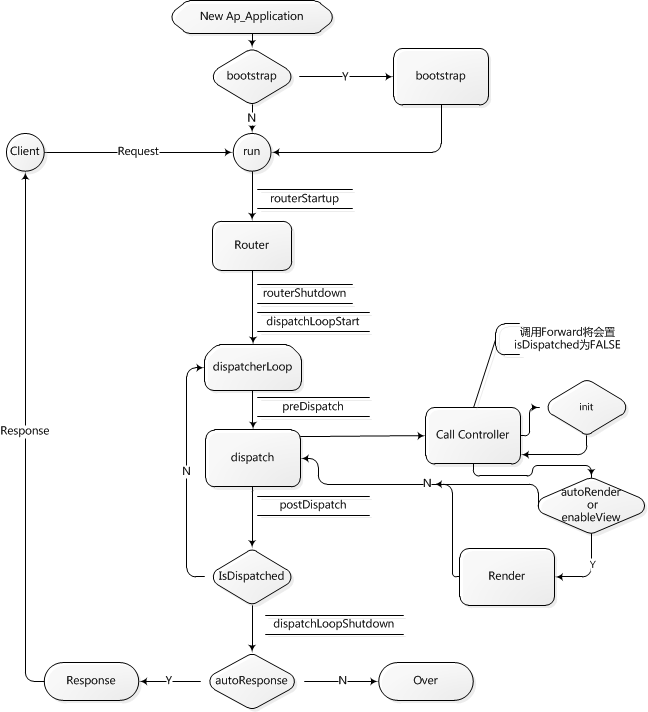
\includegraphics[scale=0.5]{yaf_sequence.png}
\caption{yaf的整体流程}
\end{figure}



\begin{lstlisting}[language=PHP]

\end{lstlisting}




\begin{lstlisting}[language=PHP]
<?php
define("APPLICATION_PATH",  dirname(__FILE__));
define("PUB_TPL",dirname(__FILE__)."/application/views");
require_once(APPLICATION_PATH."/Macro.php");
try {
	$app  = new Yaf_Application(APPLICATION_PATH."/conf/5bb88e1e53666ec494f1025023c16dea.ini");
	$app->bootstrap() //call bootstrap methods defined in Bootstrap.php
    ->run();
} catch (Yaf_Exception_StartupError $e) {

}
\end{lstlisting}




\begin{lstlisting}[language=PHP]

\end{lstlisting}



\begin{lstlisting}[language=PHP]

\end{lstlisting}




\begin{lstlisting}[language=PHP]

\end{lstlisting}




\begin{lstlisting}[language=PHP]

\end{lstlisting}




\begin{lstlisting}[language=PHP]

\end{lstlisting}




\begin{lstlisting}[language=PHP]

\end{lstlisting}









\part{Test}


\chapter{Overview}





\chapter{Server}




\section{PHP}


从PHP 5.4.0起,CLI SAPI提供了一个内置的Web服务器来用于本地开发使用,不可用于生产环境。

默认情况下,URI请求会被发送到PHP所在的的工作目录(Working Directory)进行处理,除非使用\texttt{-t}参数来自定义不同的目录。

如果请求未指定执行哪个PHP文件,则默认执行目录内的index.php 或者 index.html。如果这两个文件都不存在,服务器会返回404错误。


在命令行启动内置的Web Server时,如果指定了一个PHP文件,则这个文件会作为一个“路由”脚本,意味着每次请求都会先执行这个脚本。如果这个脚本返回 FALSE ,那么直接返回请求的文件(例如请求静态文件不作任何处理),否则会把输出返回到浏览器。

\begin{lstlisting}[language=PHP]
$ cd ~/public_html
$ php -S localhost:10086
PHP 5.6.12 Development Server started at Sun Oct 25 21:51:18 2015
Listening on http://localhost:10086
Document root is /home/test/public_html
Press Ctrl-C to quit.
\end{lstlisting}


如果需要在启动时指定Web根目录,可以执行:

\begin{lstlisting}[language=PHP]
$ cd ~/public_html
$ php -S localhost:8000 -t foo/
\end{lstlisting}


下面的示例说明如何使用路由(router)脚本,请求图片直接显示图片,请求HTML则显示“Welcome to PHP”。

\begin{lstlisting}[language=PHP]
$ cd ~/public_html
$ vim router.php
<?php
// router.php
if (preg_match('/\.(?:png|jpg|jpeg|gif)$/', $_SERVER["REQUEST_URI"]))
    return false;    // 直接返回请求的文件
else { 
    echo "<p>Welcome to PHP</p>";
}
?>
$ $ php -S localhost:8000 router.php
\end{lstlisting}

PHP内置的Web服务器能识别一些标准的MIME类型资源,例如.css, .gif, .htm, .html, .jpe, .jpeg, .jpg, .js, .png, .svg和.txt等。

对于不支持的文件类型,可以进行相应的判断和处理:



通过程序判断是否是在使用内置Web服务器,从而调整同一个PHP路由器脚本在内置Web服务器中和在生产服务器中的不同行为:


\begin{lstlisting}[language=PHP]
$ cd ~/public_html
$ vim router.php
<?php
// router.php
if (php_sapi_name() == 'cli-server') {
    /* route static assets and return false */
}
    /* go on with normal index.php operations */
?>
$ php -S localhost:10086 router.php
\end{lstlisting}




\begin{lstlisting}[language=PHP]
$ cd ~/public_html
$ vim router.php
<?php
// router.php
$path = pathinfo($_SERVER["SCRIPT_FILENAME"]);
if($path["extension"]=="ogg"){
	header("Content-Type: video/ogg");
	readfile($_SERVER["SCRIPT_FILENAME"]);
}else{
	return FALSE;
}
?>
$ php -S localhost:10086 router.php
\end{lstlisting}

如果需要开启服务器的远程访问支持,可以执行:

\begin{lstlisting}[language=PHP]
$ php -S 0.0.0.0:10086
\end{lstlisting}




\begin{lstlisting}[language=PHP]

\end{lstlisting}



\begin{lstlisting}[language=PHP]

\end{lstlisting}




\begin{lstlisting}[language=PHP]

\end{lstlisting}




\begin{lstlisting}[language=PHP]

\end{lstlisting}




\begin{lstlisting}[language=PHP]

\end{lstlisting}




\begin{lstlisting}[language=PHP]

\end{lstlisting}





\begin{lstlisting}[language=PHP]

\end{lstlisting}











\section{Python}


Python自带的Web服务器SimpleHTTPServer可以使用下面的命令来启动(端口号默认为8000):



\begin{lstlisting}[language=PHP]
python -m Web服务器模块 [端口号,默认8000]
\end{lstlisting}


这里的“Web服务器模块”有如下3种:

\begin{compactitem}
\item BaseHTTPServer: 提供基本的Web服务和处理器类,分别是HTTPServer和BaseHTTPRequestHandler。
\item SimpleHTTPServer: 包含执行GET和HEAD请求的SimpleHTTPRequestHandler类。
\item CGIHTTPServer: 包含处理POST请求和执行CGIHTTPRequestHandler类。
\end{compactitem}

\begin{lstlisting}[language=PHP]
$ cd ~/public_html
$ python -m SimpleHTTPServer 10086
\end{lstlisting}

\begin{lstlisting}[language=PHP]

\end{lstlisting}




\begin{lstlisting}[language=PHP]

\end{lstlisting}




\begin{lstlisting}[language=PHP]

\end{lstlisting}




\begin{lstlisting}[language=PHP]

\end{lstlisting}





\begin{lstlisting}[language=PHP]

\end{lstlisting}




\begin{lstlisting}[language=PHP]

\end{lstlisting}







\begin{lstlisting}[language=PHP]

\end{lstlisting}




\begin{lstlisting}[language=PHP]

\end{lstlisting}




\begin{lstlisting}[language=PHP]

\end{lstlisting}




\begin{lstlisting}[language=PHP]

\end{lstlisting}




\begin{lstlisting}[language=PHP]

\end{lstlisting}





\begin{lstlisting}[language=PHP]

\end{lstlisting}




\begin{lstlisting}[language=PHP]

\end{lstlisting}







\begin{lstlisting}[language=PHP]

\end{lstlisting}




\begin{lstlisting}[language=PHP]

\end{lstlisting}




\begin{lstlisting}[language=PHP]

\end{lstlisting}




\begin{lstlisting}[language=PHP]

\end{lstlisting}




\begin{lstlisting}[language=PHP]

\end{lstlisting}





\begin{lstlisting}[language=PHP]

\end{lstlisting}




\begin{lstlisting}[language=PHP]

\end{lstlisting}







\begin{lstlisting}[language=PHP]

\end{lstlisting}




\begin{lstlisting}[language=PHP]

\end{lstlisting}




\begin{lstlisting}[language=PHP]

\end{lstlisting}




\begin{lstlisting}[language=PHP]

\end{lstlisting}




\begin{lstlisting}[language=PHP]

\end{lstlisting}





\begin{lstlisting}[language=PHP]

\end{lstlisting}




\begin{lstlisting}[language=PHP]

\end{lstlisting}







\begin{lstlisting}[language=PHP]

\end{lstlisting}




\begin{lstlisting}[language=PHP]

\end{lstlisting}




\begin{lstlisting}[language=PHP]

\end{lstlisting}




\begin{lstlisting}[language=PHP]

\end{lstlisting}




\begin{lstlisting}[language=PHP]

\end{lstlisting}





\begin{lstlisting}[language=PHP]

\end{lstlisting}




\begin{lstlisting}[language=PHP]

\end{lstlisting}









\part{Release}



\part{Security}


\chapter{Overview}

在OSI(开放系统互联)模型的第七层——应用层向用户的应用程序提供网络服务等。

在实际的网络环境中,仅仅加固网络设备无法防止攻击者通过网络对系统中的Web应用的攻击,而且攻击者可以先入侵目标系统的应用层,然后再伺机进入系统内部。

OWASP开放社区提供了安全编码原则和实践来提高产品的安全性,而且OWASP通过评估攻击向量和安全隐患归纳出的应用安全风险可以涵盖通用的攻击方法,和目标所使用的平台和技术无关,而且OSASP还提供了测试、验证和修复漏洞的指导方案。

\section{Injection}


注入(Injection)是指攻击者通过输入恶意数据来实现在Web服务器中运行任意指令的目的,例如SQL、XML和LDAP注入等。

在应用程序中,通过对用户输入的特定字符进行转义,可以预防恶意数据注入。

\section{XSS}


跨站脚本(Cross-Site Scripting,XSS)是指应用程序在没有对用户输入进行正确验证的情况下,将这些输入直接输出到Web浏览器中,并且在浏览器中执行来实现会话劫持、cookie窃取或者Web站点数据污染等。

在应用程序中,通过对HTML、JavaScript或者CSS输出中不受信任的元字符进行转义,可以预防XSS攻击。


\section{Authentication}

无效的验证和会话管理可以导致用户账户被劫持,或者导致会话token可预测等。

在开发健壮的验证和会话管理程序时,建议使用加密、散列和基于SSL/TLS的安全数据连接。


\section{Reference}

如果应用程序提供其内部对象的直接引用,并且没有进行正确验证,就可能导致攻击者操纵这些引用并访问未经授权的数据。

内部对象可能是用户账户的参数值、文件名或目录,在访问控制检查完成之前限制所有用户可以访问的内部对象,可以确保对相关对象的每一次访问都是经过验证的。

\section{CSRF}

跨站请求伪造(Crosss-Site Request Forgery,CSRF)是指在存在漏洞的Web应用中,强迫经过验证的用户去运行伪造的HTTP请求。

HTTP恶意请求都是在合法的用户会话中被执行的,因此无法检测,在实践中通过在每一个用户会话中都生成一个ie不可预测的token,然后每次发送HTTP请求时都绑定这个token,可以减轻CSRF攻击的危害。

\section{Misconfiguration}

在生产环境中使用默认的额安全配置可能会导致应用程序遭受多种攻击,因此在已部署的应用、Web服务区、数据库服务器、操作系代码库以及所有和应用程序相关的组件中,都应该使用现有的最佳安全配置,并且通过不断地进行软件更新、打补丁和严格执行应用环境中的安全规则来实现安全的应用程序配置。

\section{Cryptography}

如果在应用程序中没有对敏感数据(例如医保信息、信用卡交易、个人信息和认证细节等)使用密码保护机制,那么就可以产生密码泄露等危害。

用户可以使用健壮的加密算法或散列算法来保证敏感数据的安全性。

\section{URL}

如果Web应用程序没有对URL的访问进行权限检查,那么攻击者可能可以访问呢未经授权的网页。

为了防范失败的URL访问权限,需要使用合适的身份证明和授权控制机制来限制对私有URL的访问,同时需要为那些可以访问高敏感性数据的特殊用户和角色开发适当的权限控制策略。

\section{Transport}

低强度的加密算法、无效的安全证书以及不恰当的身份证明控制机制都可能会破坏数据的机密性和完整性,从而使应用数据遭到流量窃听和篡改攻击。

在传输所有敏感网页时使用SSL/TLS协议,并使用权威认证机构办法的合法数字证书,可以解决薄弱的传输层保护问题。

\section{Validation}

如果Web应用程序使用动态参数来将用户重定向或跳转到某个特定的URL上,攻击者就可以通过相同的方法伪造一个恶意的URL来将用户重定向到钓鱼网站或恶意网站上。

未验证的重定向和转发攻击还可以用来将请求转发到本地未经授权的网页上,因此需要验证请求中的参数和发出请求的用户的访问权限来避免非法重定向和转发。



































\end{document}












